\documentclass[12pt, parskip=half, a4paper, oneside]{scrartcl}
\usepackage[ngerman]{babel}
\usepackage[utf8]{inputenc}
\usepackage{amsmath, amssymb, amsfonts}
\usepackage{lmodern, clock, graphicx, units, textcomp, multicol, booktabs}
\usepackage[Smaller]{cancel}
\usepackage{xlop}
\usepackage[left=2.5cm, right=0.5cm, top=1cm, bottom=0.5cm]{geometry}
\usepackage{icomma, paralist, array}

\usepackage{wasysym, pifont,xstring}      % Vierecke zum Ankreuzen (\Square) und bereits gekreuzte Vierecke (\XBox)

\usepackage[clock]{ifsym} % Uhrsymbol

%\usepackage{pstricks, pst-plot, pstricks-add, pst-math, pst-func, pst-all}

\renewcommand{\d}{\text{\, d}}
\newcommand{\e}{\text{e}}

\setkomafont{section}{\sffamily\huge\centering}
\setkomafont{subsection}{\normalfont\large\centering}

\newcounter{aufgabe}
\setcounter{aufgabe}{0}

\newcommand{\aufgabe}{\paragraph{Aufgabe \arabic{aufgabe}:}\stepcounter{aufgabe}}

\KOMAoptions{numbers=noenddot}

%Kopf und Fusszeilen definieren
\usepackage{scrlayer-scrpage}
\clearpairofpagestyles
\setkomafont{pageheadfoot}{\sffamily}
\setkomafont{pagination}{}

 
%\ohead[6. Oktober 2017]{6. Oktober 2017} 
%\ihead[Name, Vorname:]{Name,Vorname:} 
%\chead[Seite \arabic{page}]{Seite \arabic{page}}
% 
%\KOMAoptions{headsepline=true}\setheadsepline[\textwidth+1.5cm]{ 0.8pt}[\hspace*{-0.75cm}\centering]

\allowdisplaybreaks[1]

\let\v\vec

\renewcommand{\d}{\text\textdegree}

\renewcommand{\t}[1]{\text{\tiny{#1}}}
\newcommand{\sq}{\text{\raisebox{-0.3ex}{\huge\Square~}}}
\newcommand{\sa}{\raisebox{-1.5ex}{\rule{0pt}{0.7cm}}}
\newcommand{\sd}{{\Large\hspace*{-0.5ex}\textcolor{white}{I}}}

\newcolumntype{C}[1]{>{\centering\arraybackslash}m{#1}}

\let\E\texteuro
\let\nf\nicefrac

\newcount\tmpnum
\def\tallymarks#1{\leavevmode \lower1bp\vbox to9bp{}%
   \tmpnum=#1
   \loop \ifnum\tmpnum<5 \kern1bp \tallynum\tmpnum \else \tallyV \fi
         \advance\tmpnum by-5
         \ifnum\tmpnum>0 \repeat
}
\def\tallynum#1{\bgroup\tmpnum=#1\relax
   \loop \ifnum\tmpnum>0
         \kern1bp \tallyI \kern1bp
         \advance\tmpnum by-1
         \repeat
   \egroup
}
\def\tallyI{\pdfliteral{q .5 w 0 -1 m 0 8 l S Q}}
\def\tallyV{\kern1bp\pdfliteral{q .5 w -1 0 m 9 7 l S Q}\tallynum4\kern1bp }

\usepackage{tikz}
\usetikzlibrary{shapes.misc}
\usetikzlibrary{arrows.meta}
\usetikzlibrary{angles,quotes}
%\usetikzlibrary{intersections}
\usetikzlibrary{calc}
\usetikzlibrary{decorations.text}

\begin{document}
\section*{Ganzrationale Funktionen}
Notiere für jede Funktion die Anzahl der Nullstellen und das Unendlichkeitsverhalten!

\paragraph{Grad 1:}\textcolor{white}{.}

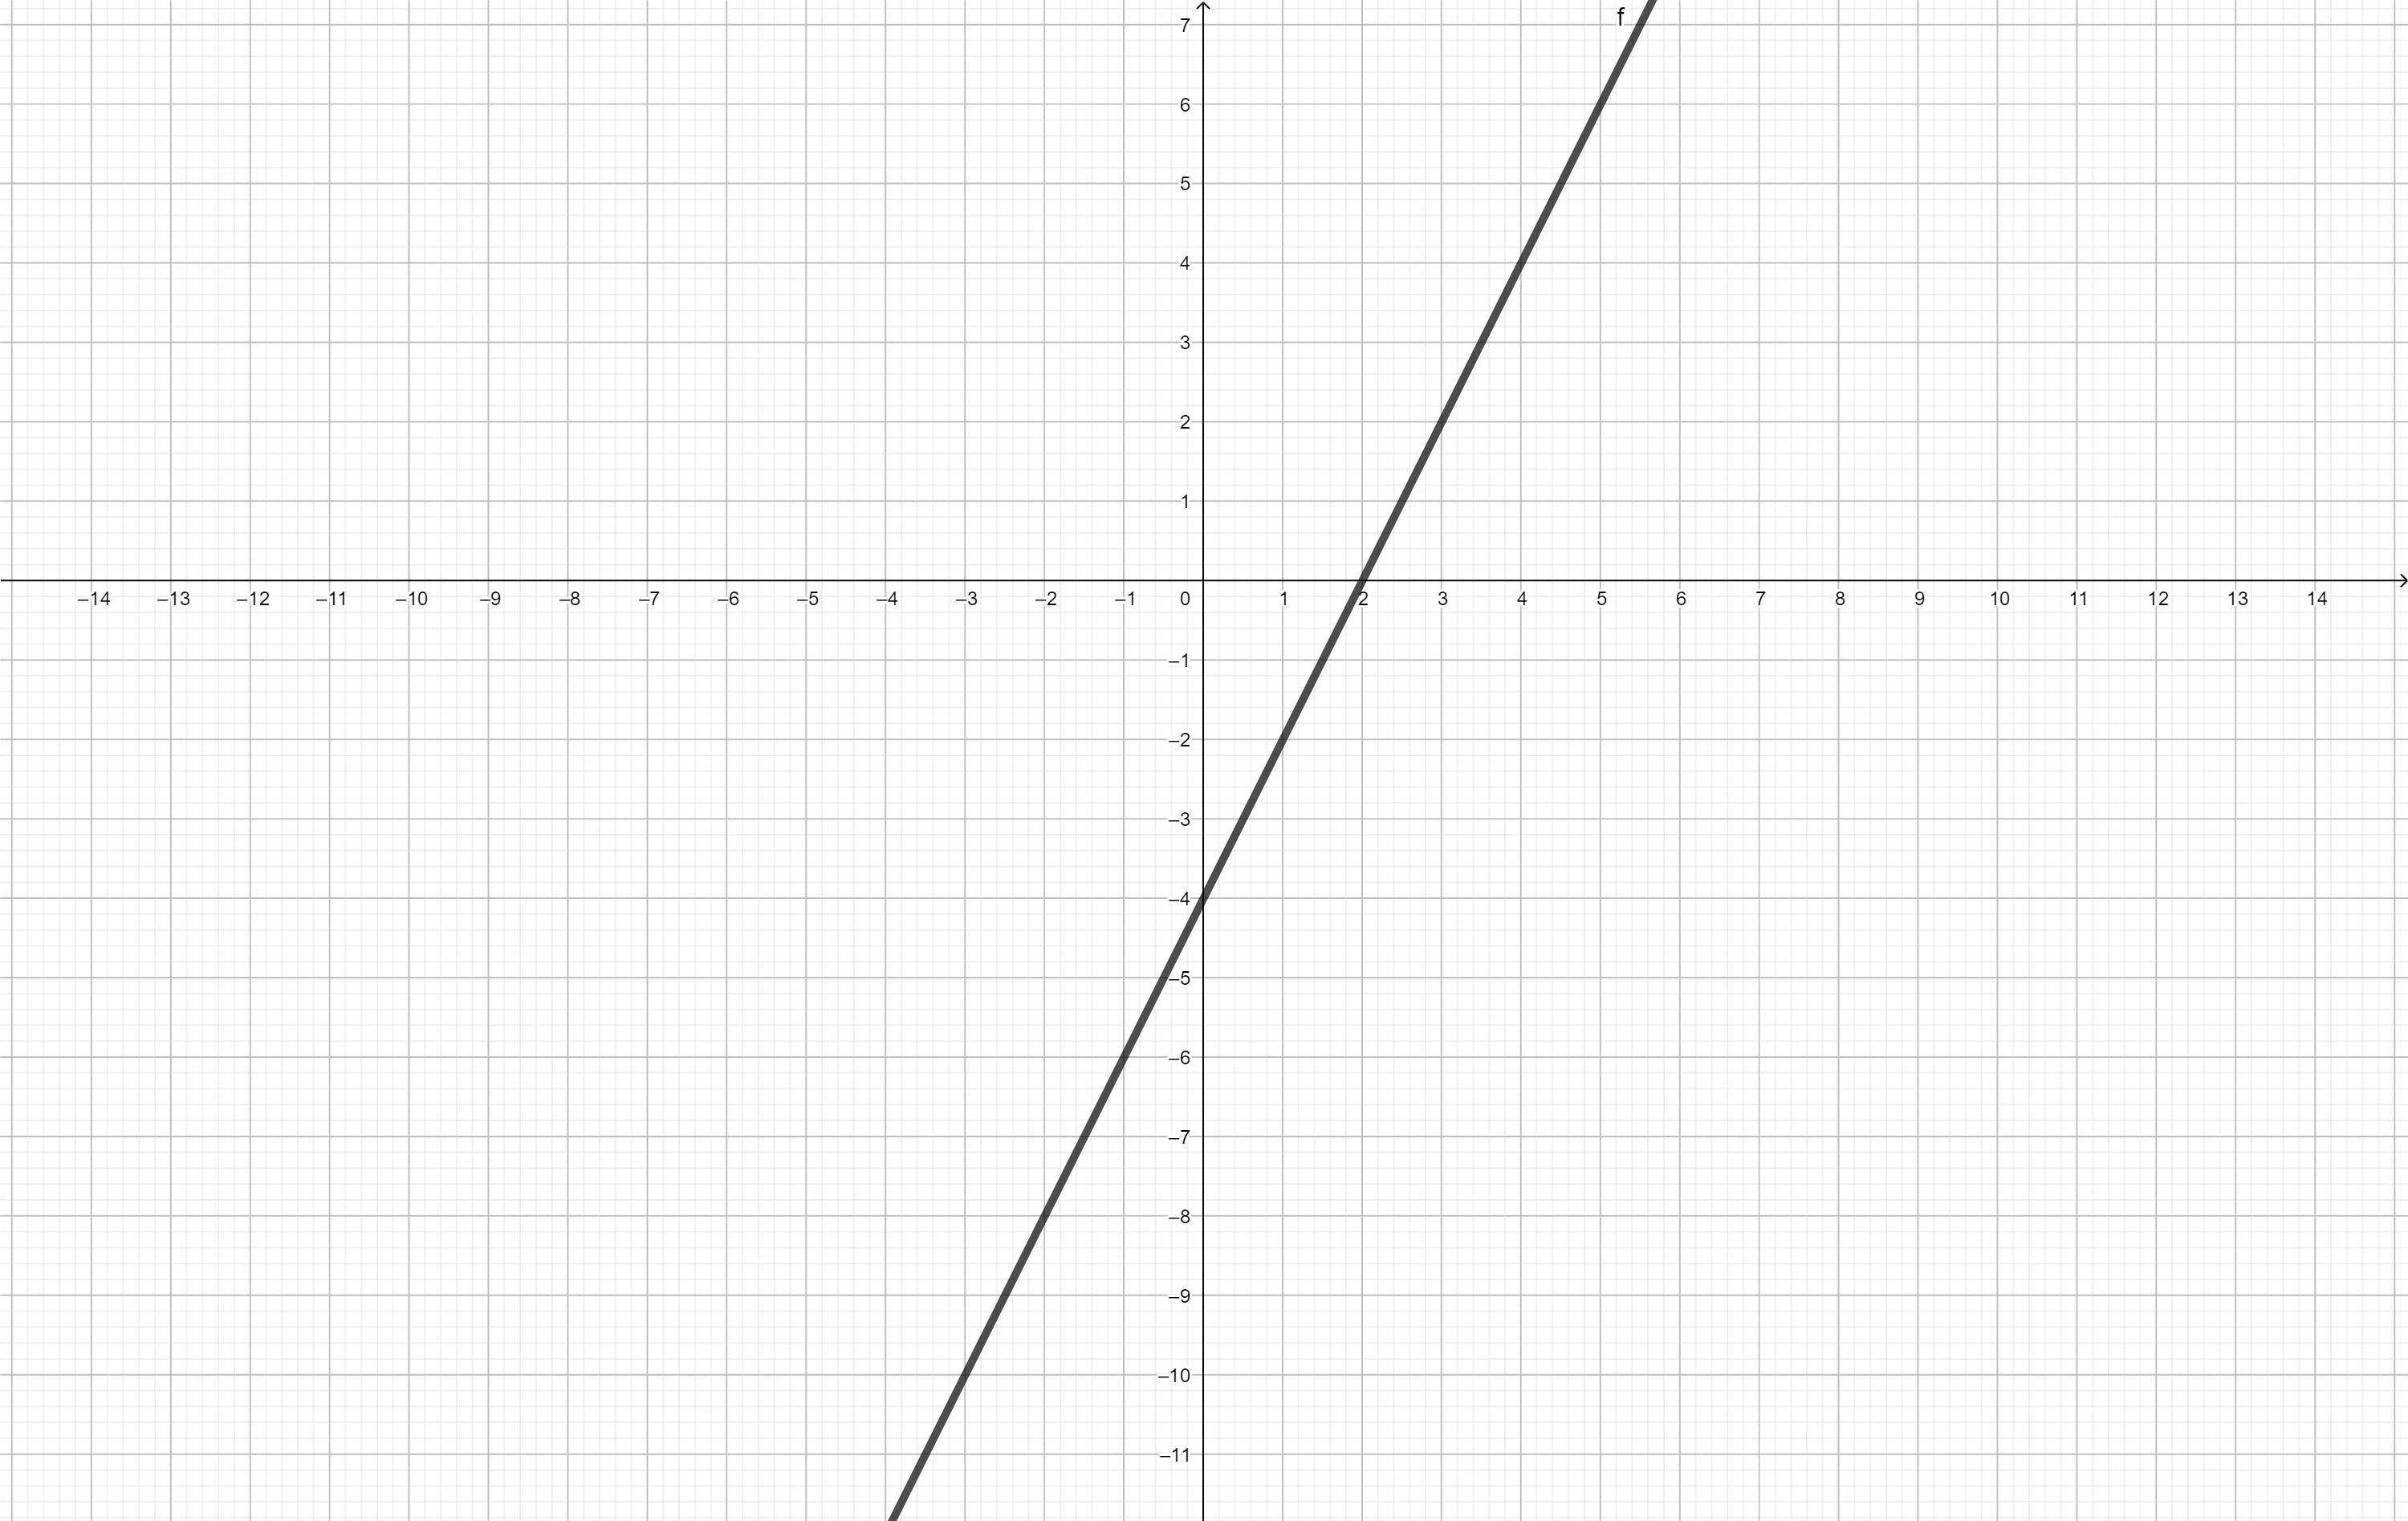
\includegraphics[width=4cm]{Bilder/G11}\hfill
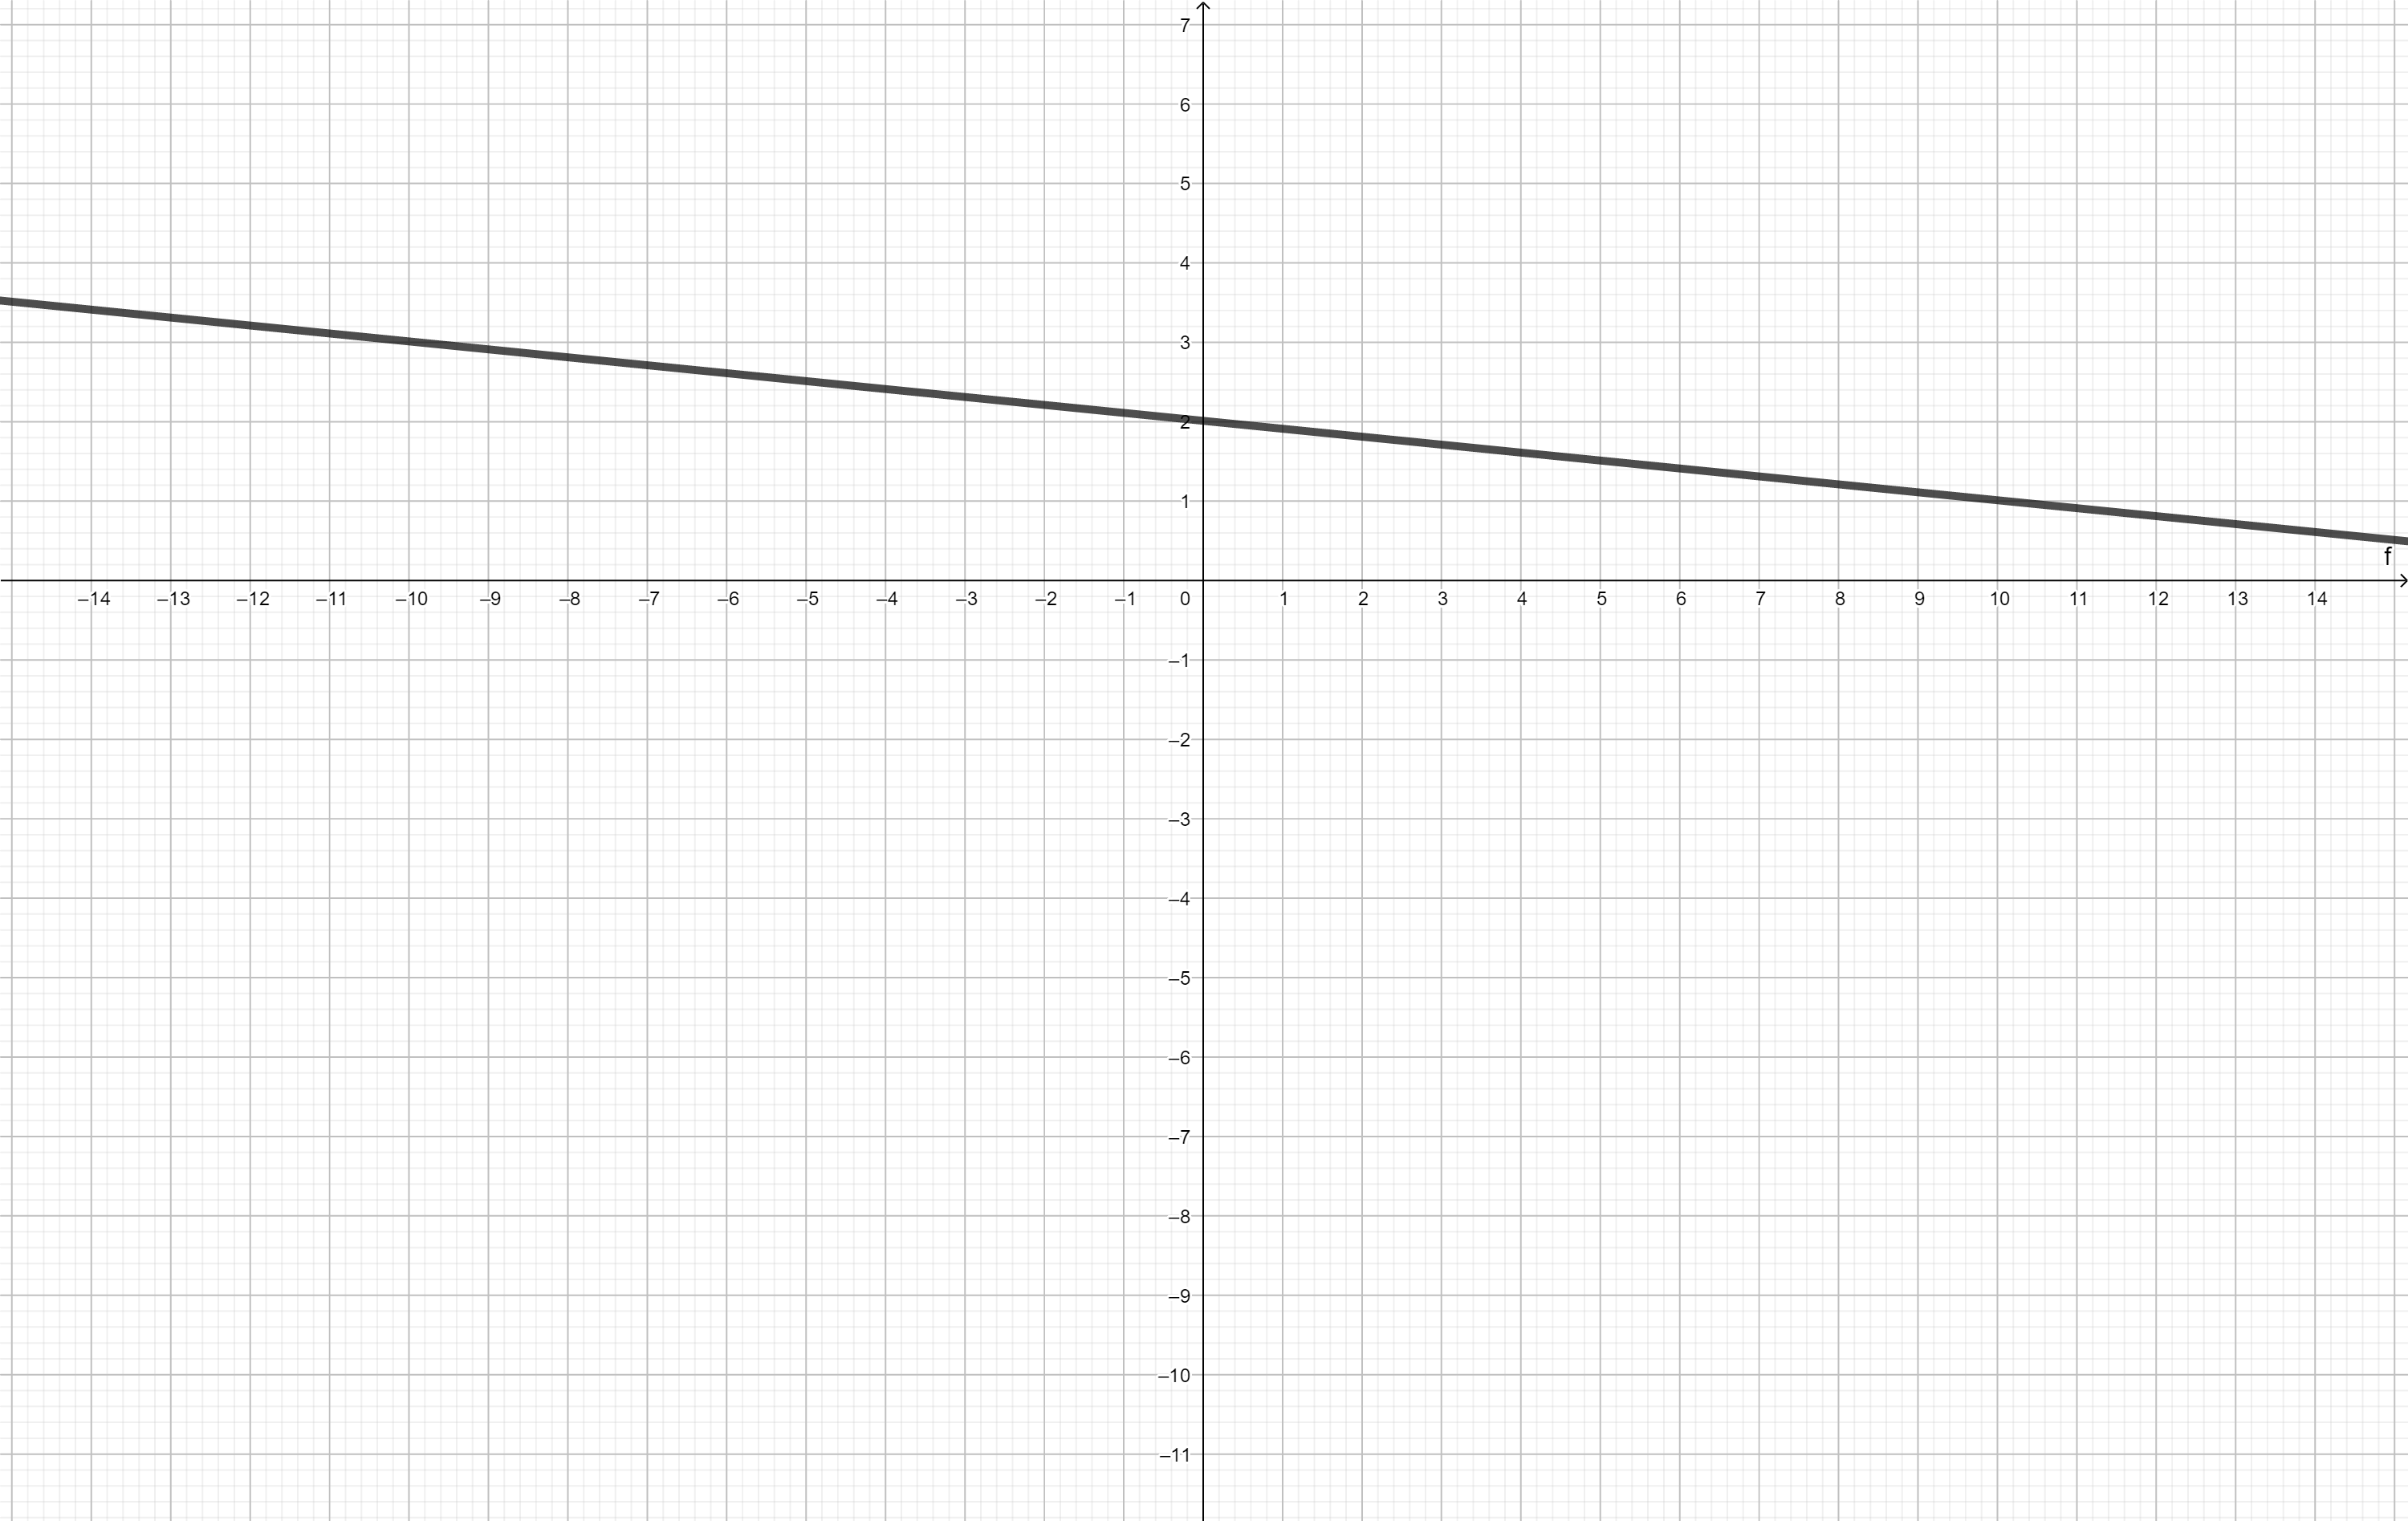
\includegraphics[width=4cm]{Bilder/G12}\hfill
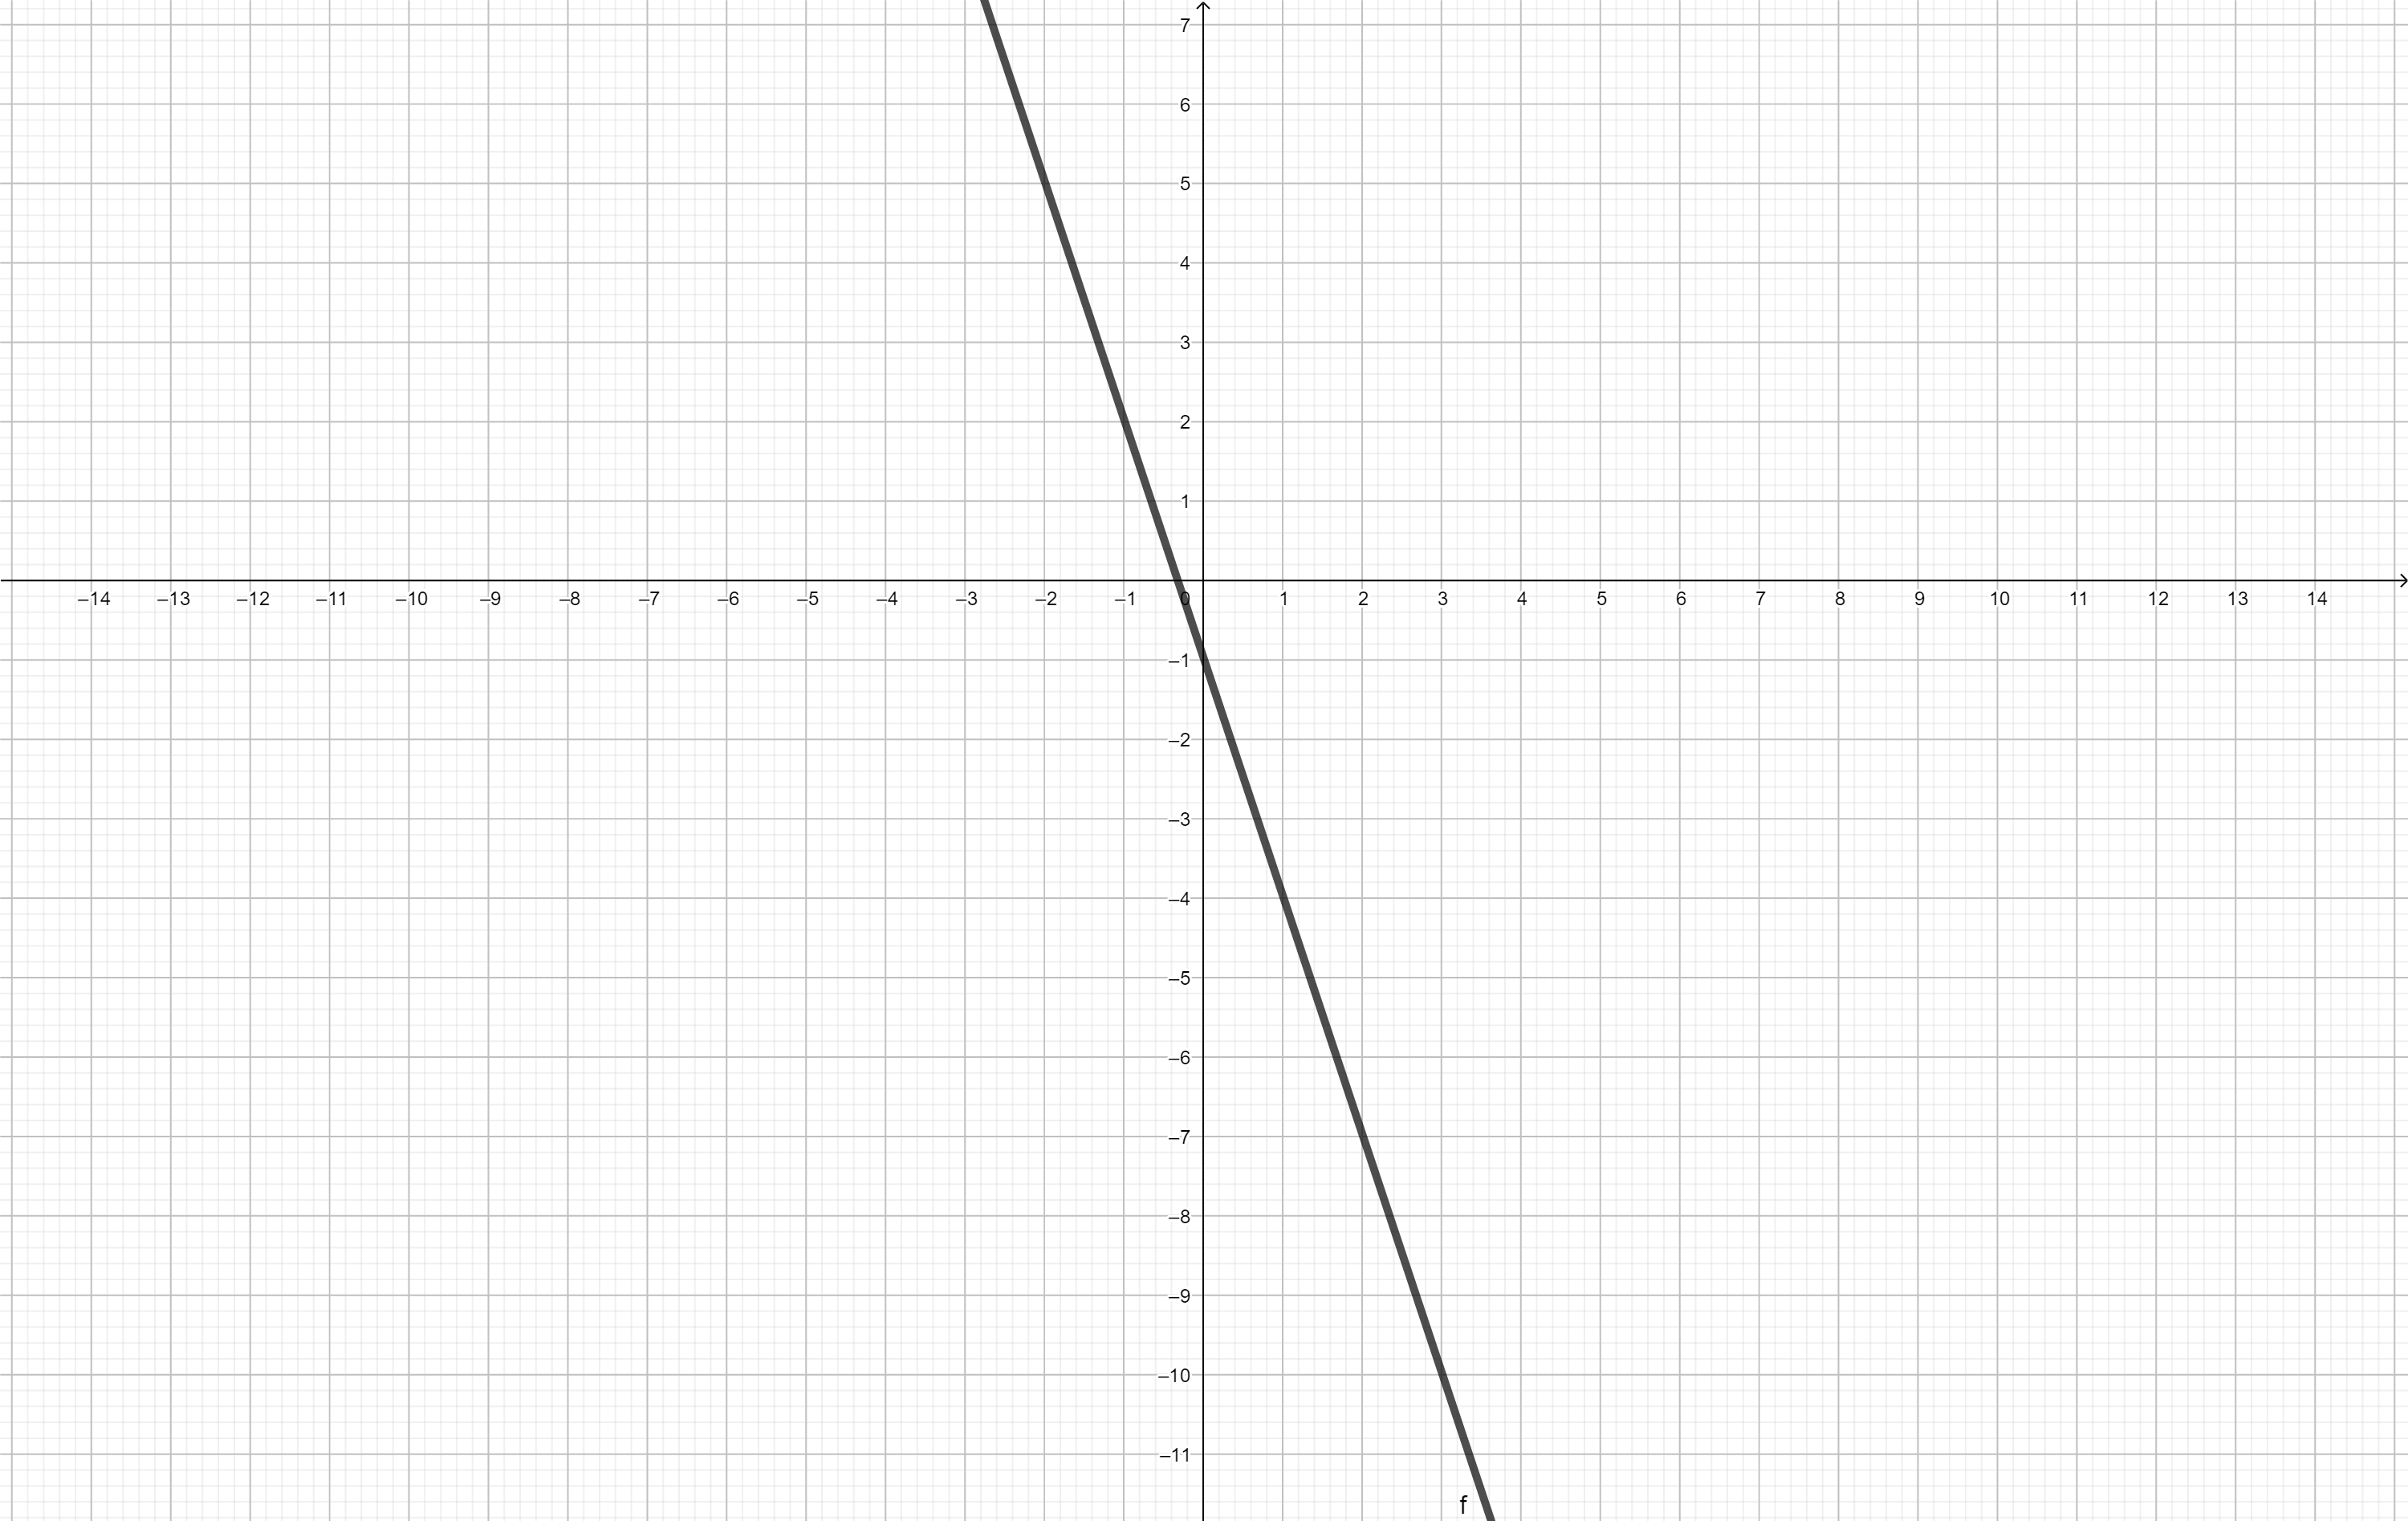
\includegraphics[width=4cm]{Bilder/G13}\hfill
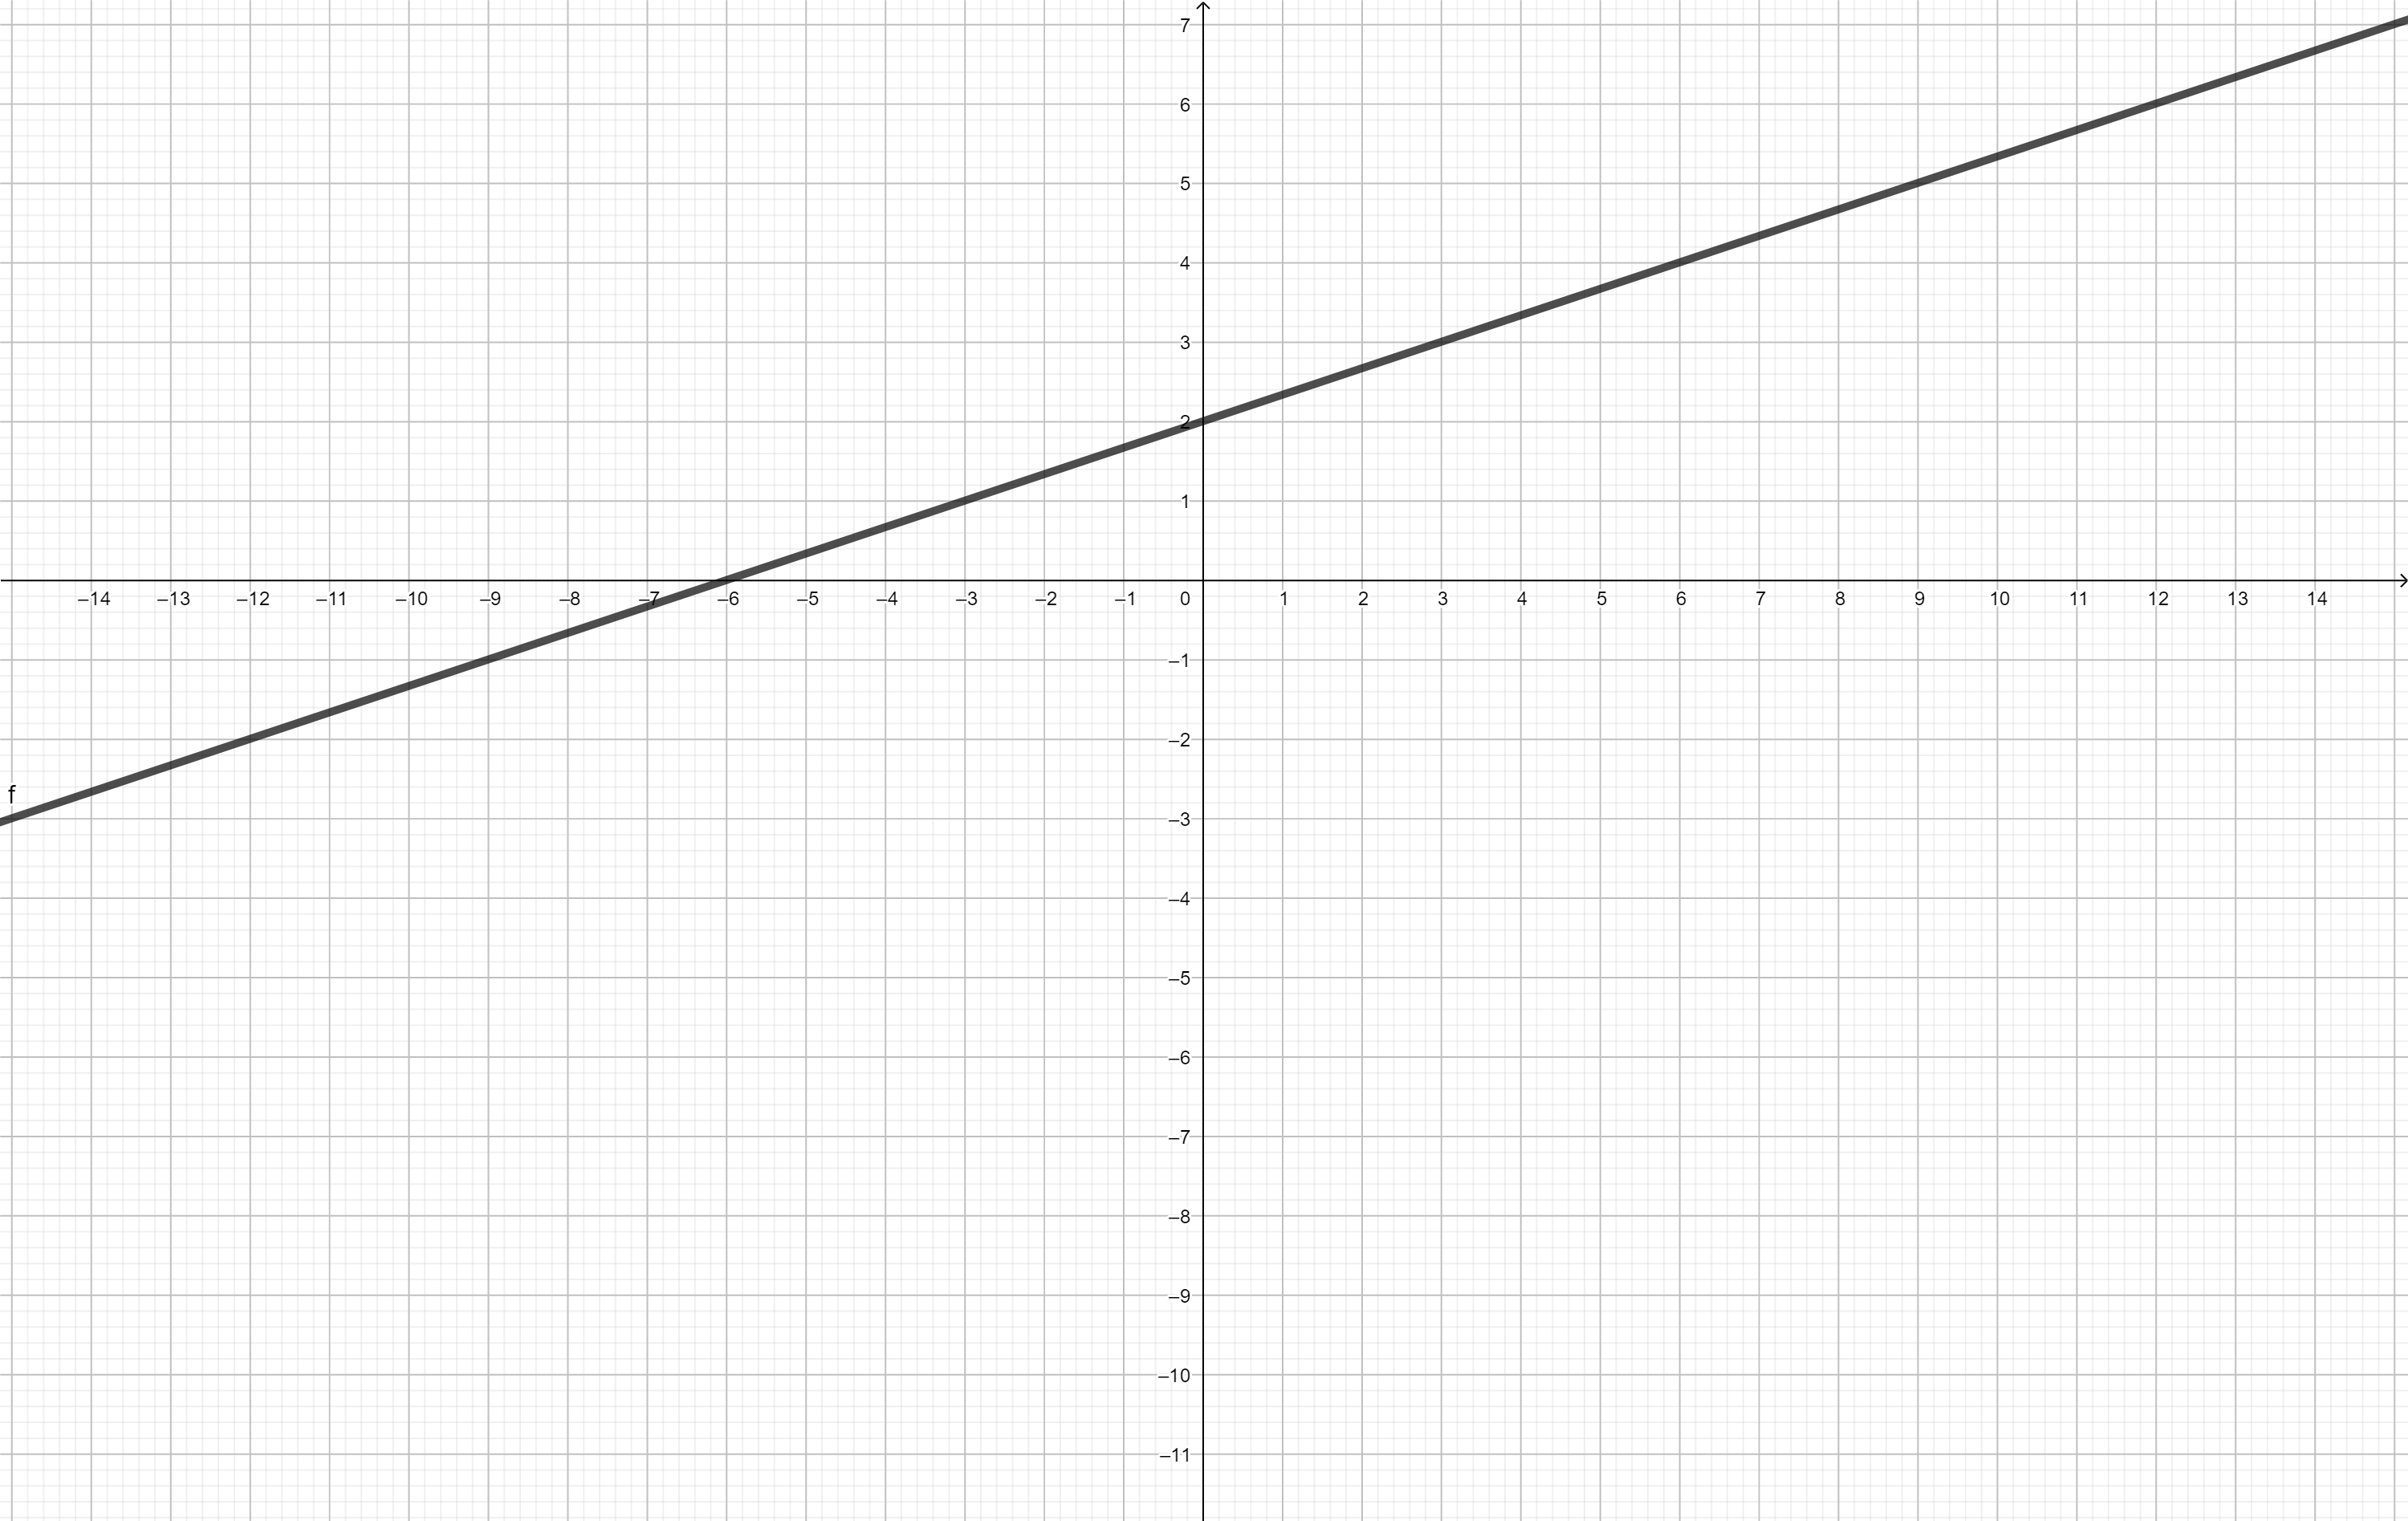
\includegraphics[width=4cm]{Bilder/G14}

\begin{addmargin}[-2cm]{0pt}
Nullstellen:

$x\rightarrow\infty:$

$x\rightarrow-\infty:$
\end{addmargin}

\paragraph{Grad 2:}\textcolor{white}{.}

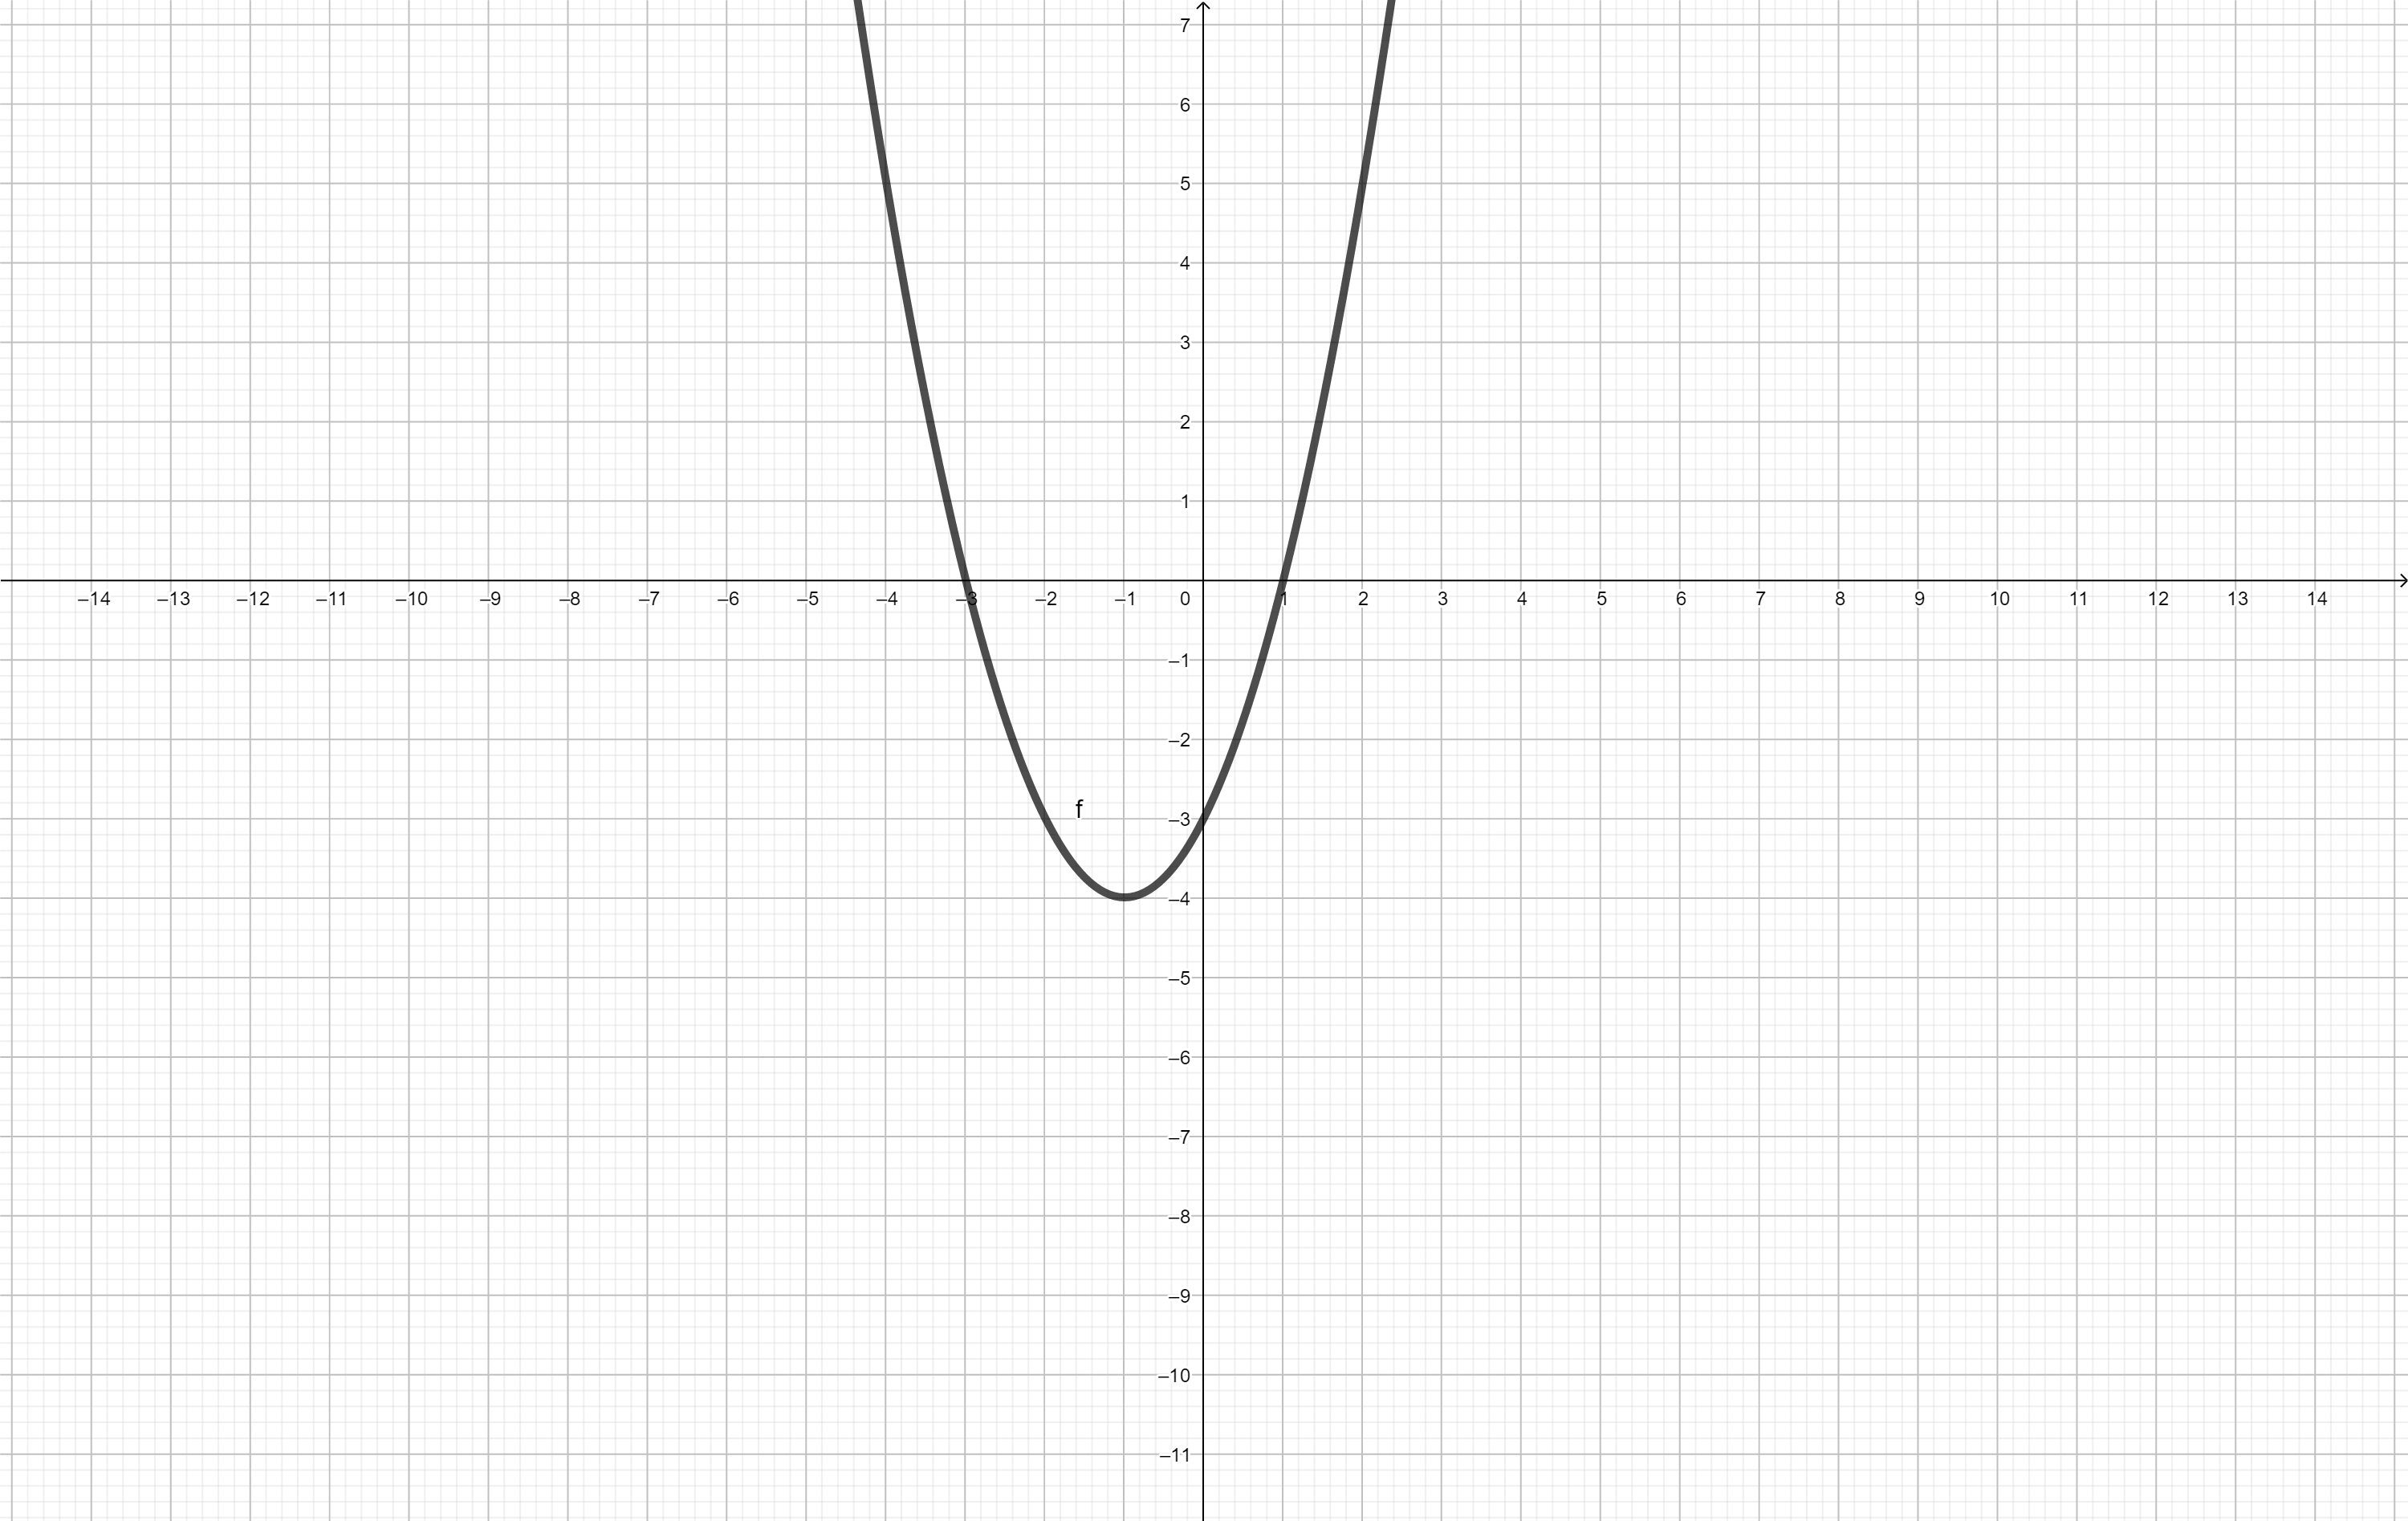
\includegraphics[width=4cm]{Bilder/G21}\hfill
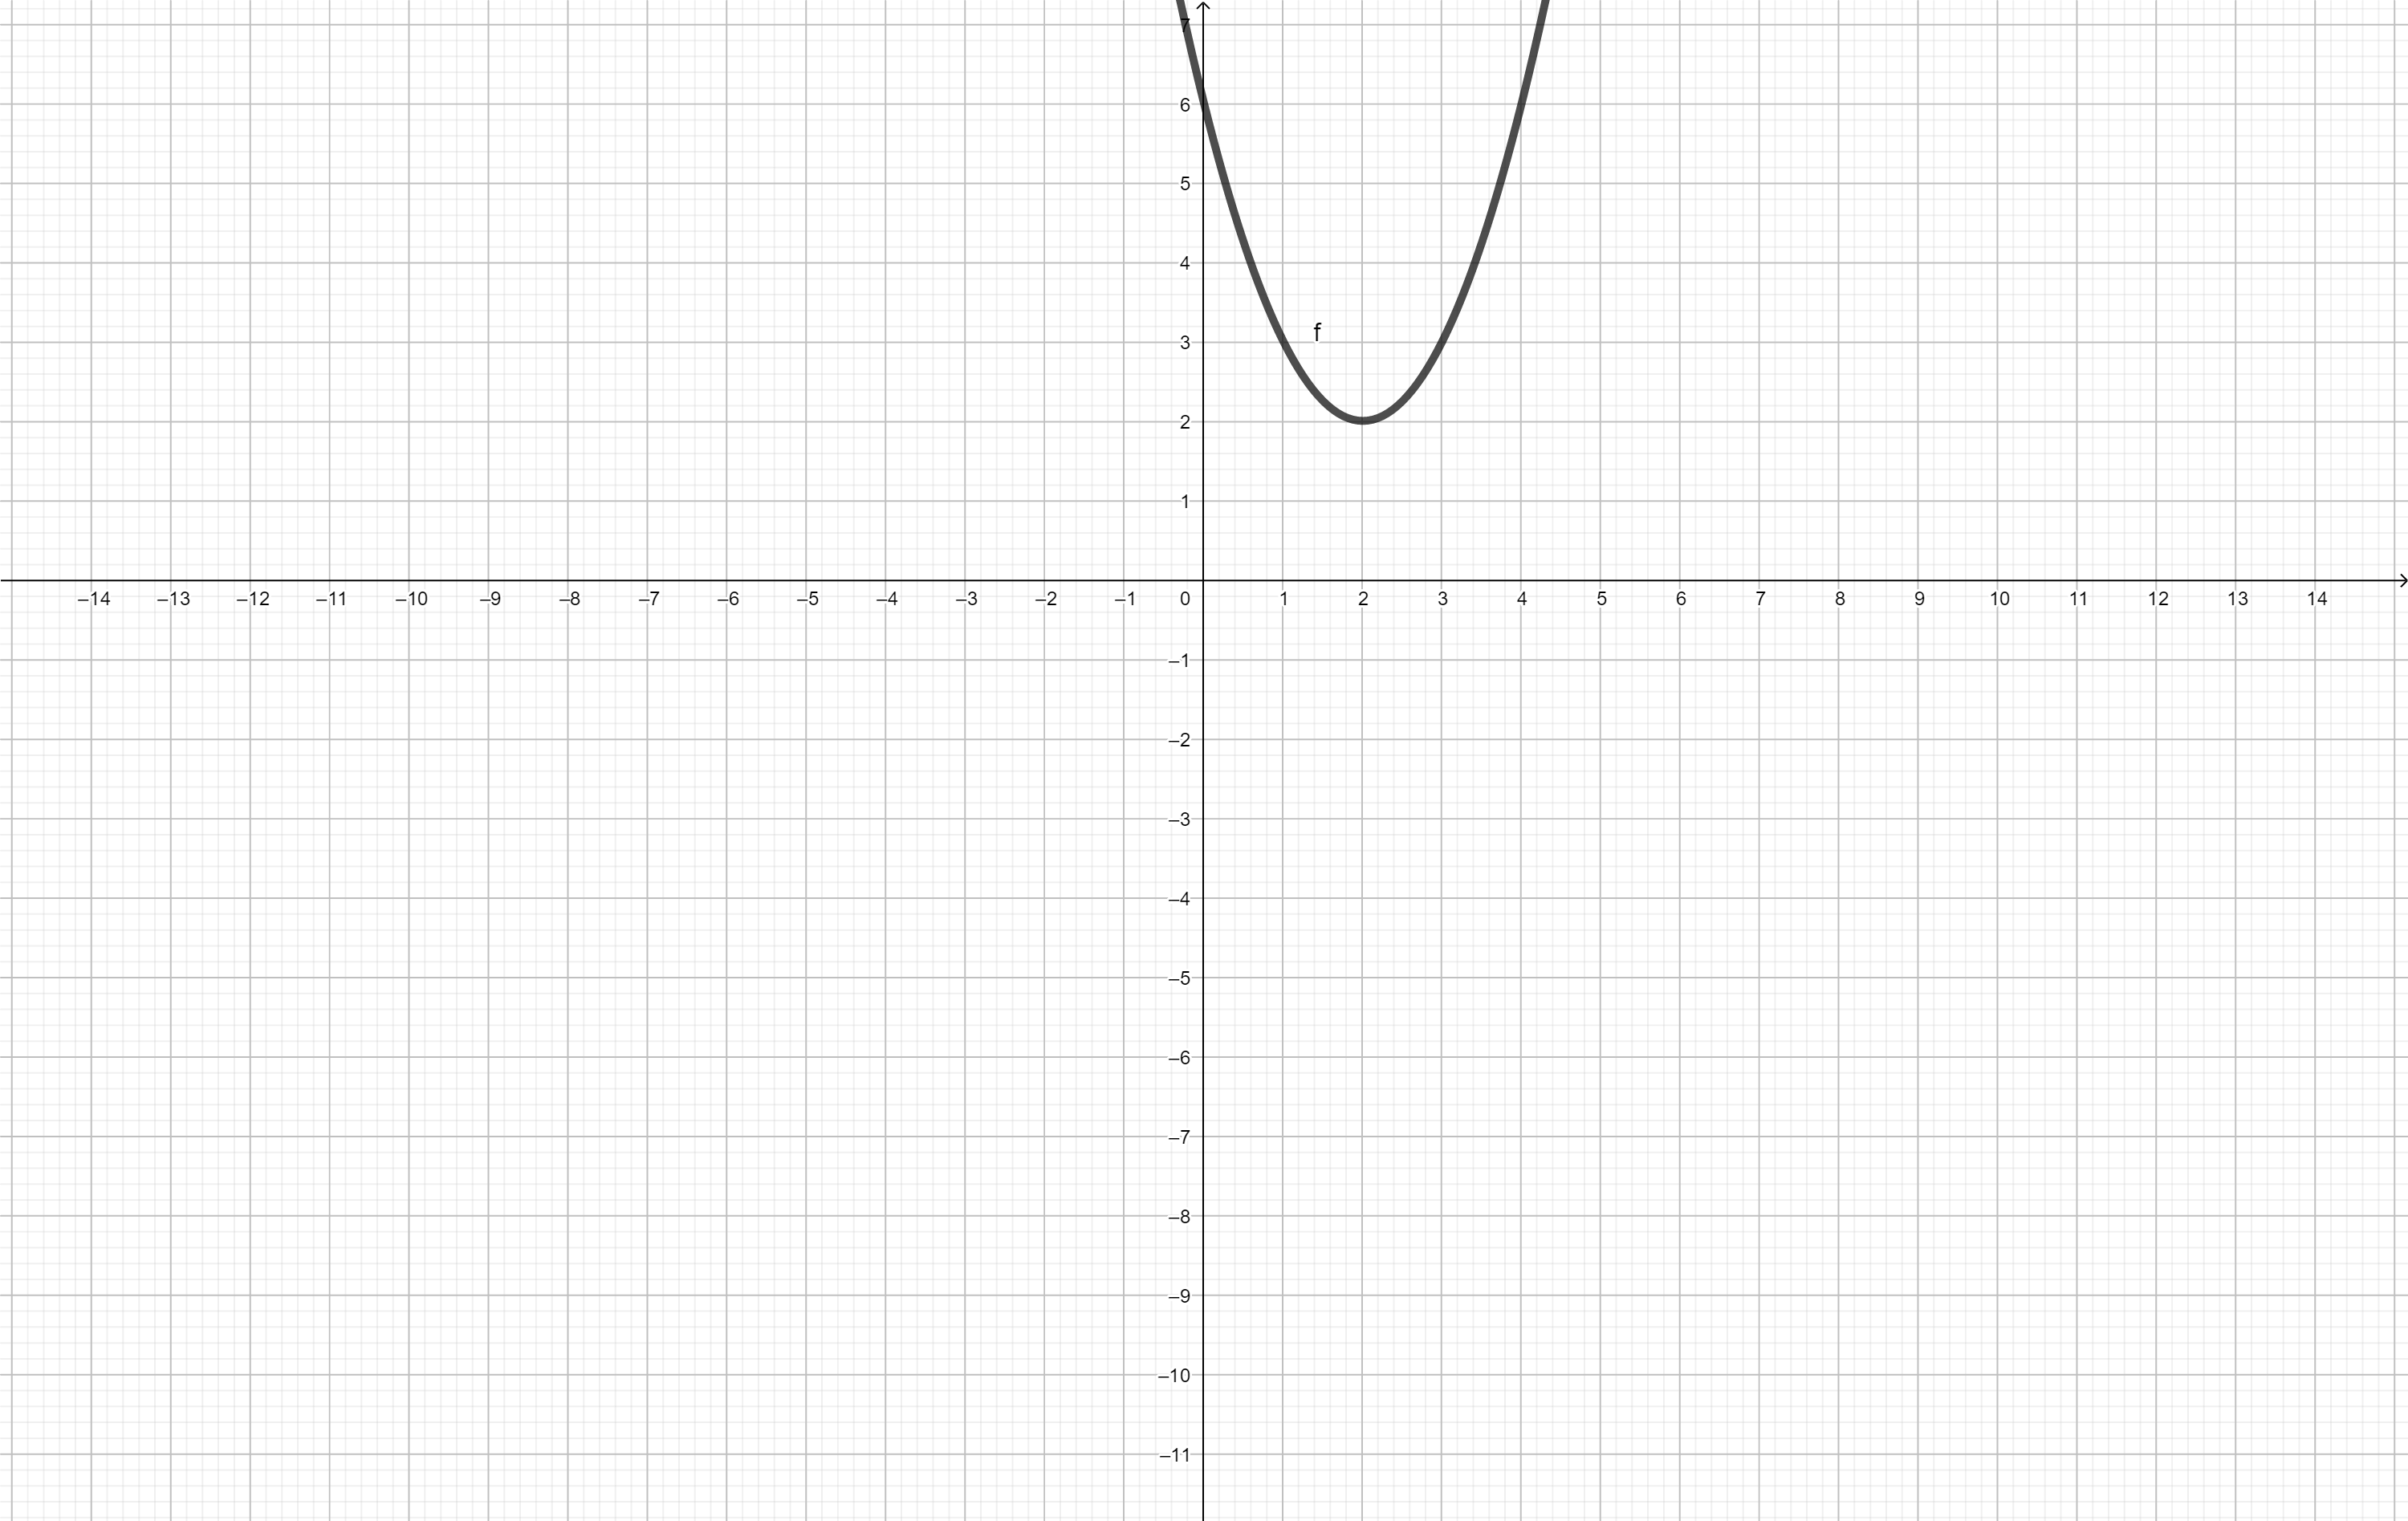
\includegraphics[width=4cm]{Bilder/G22}\hfill
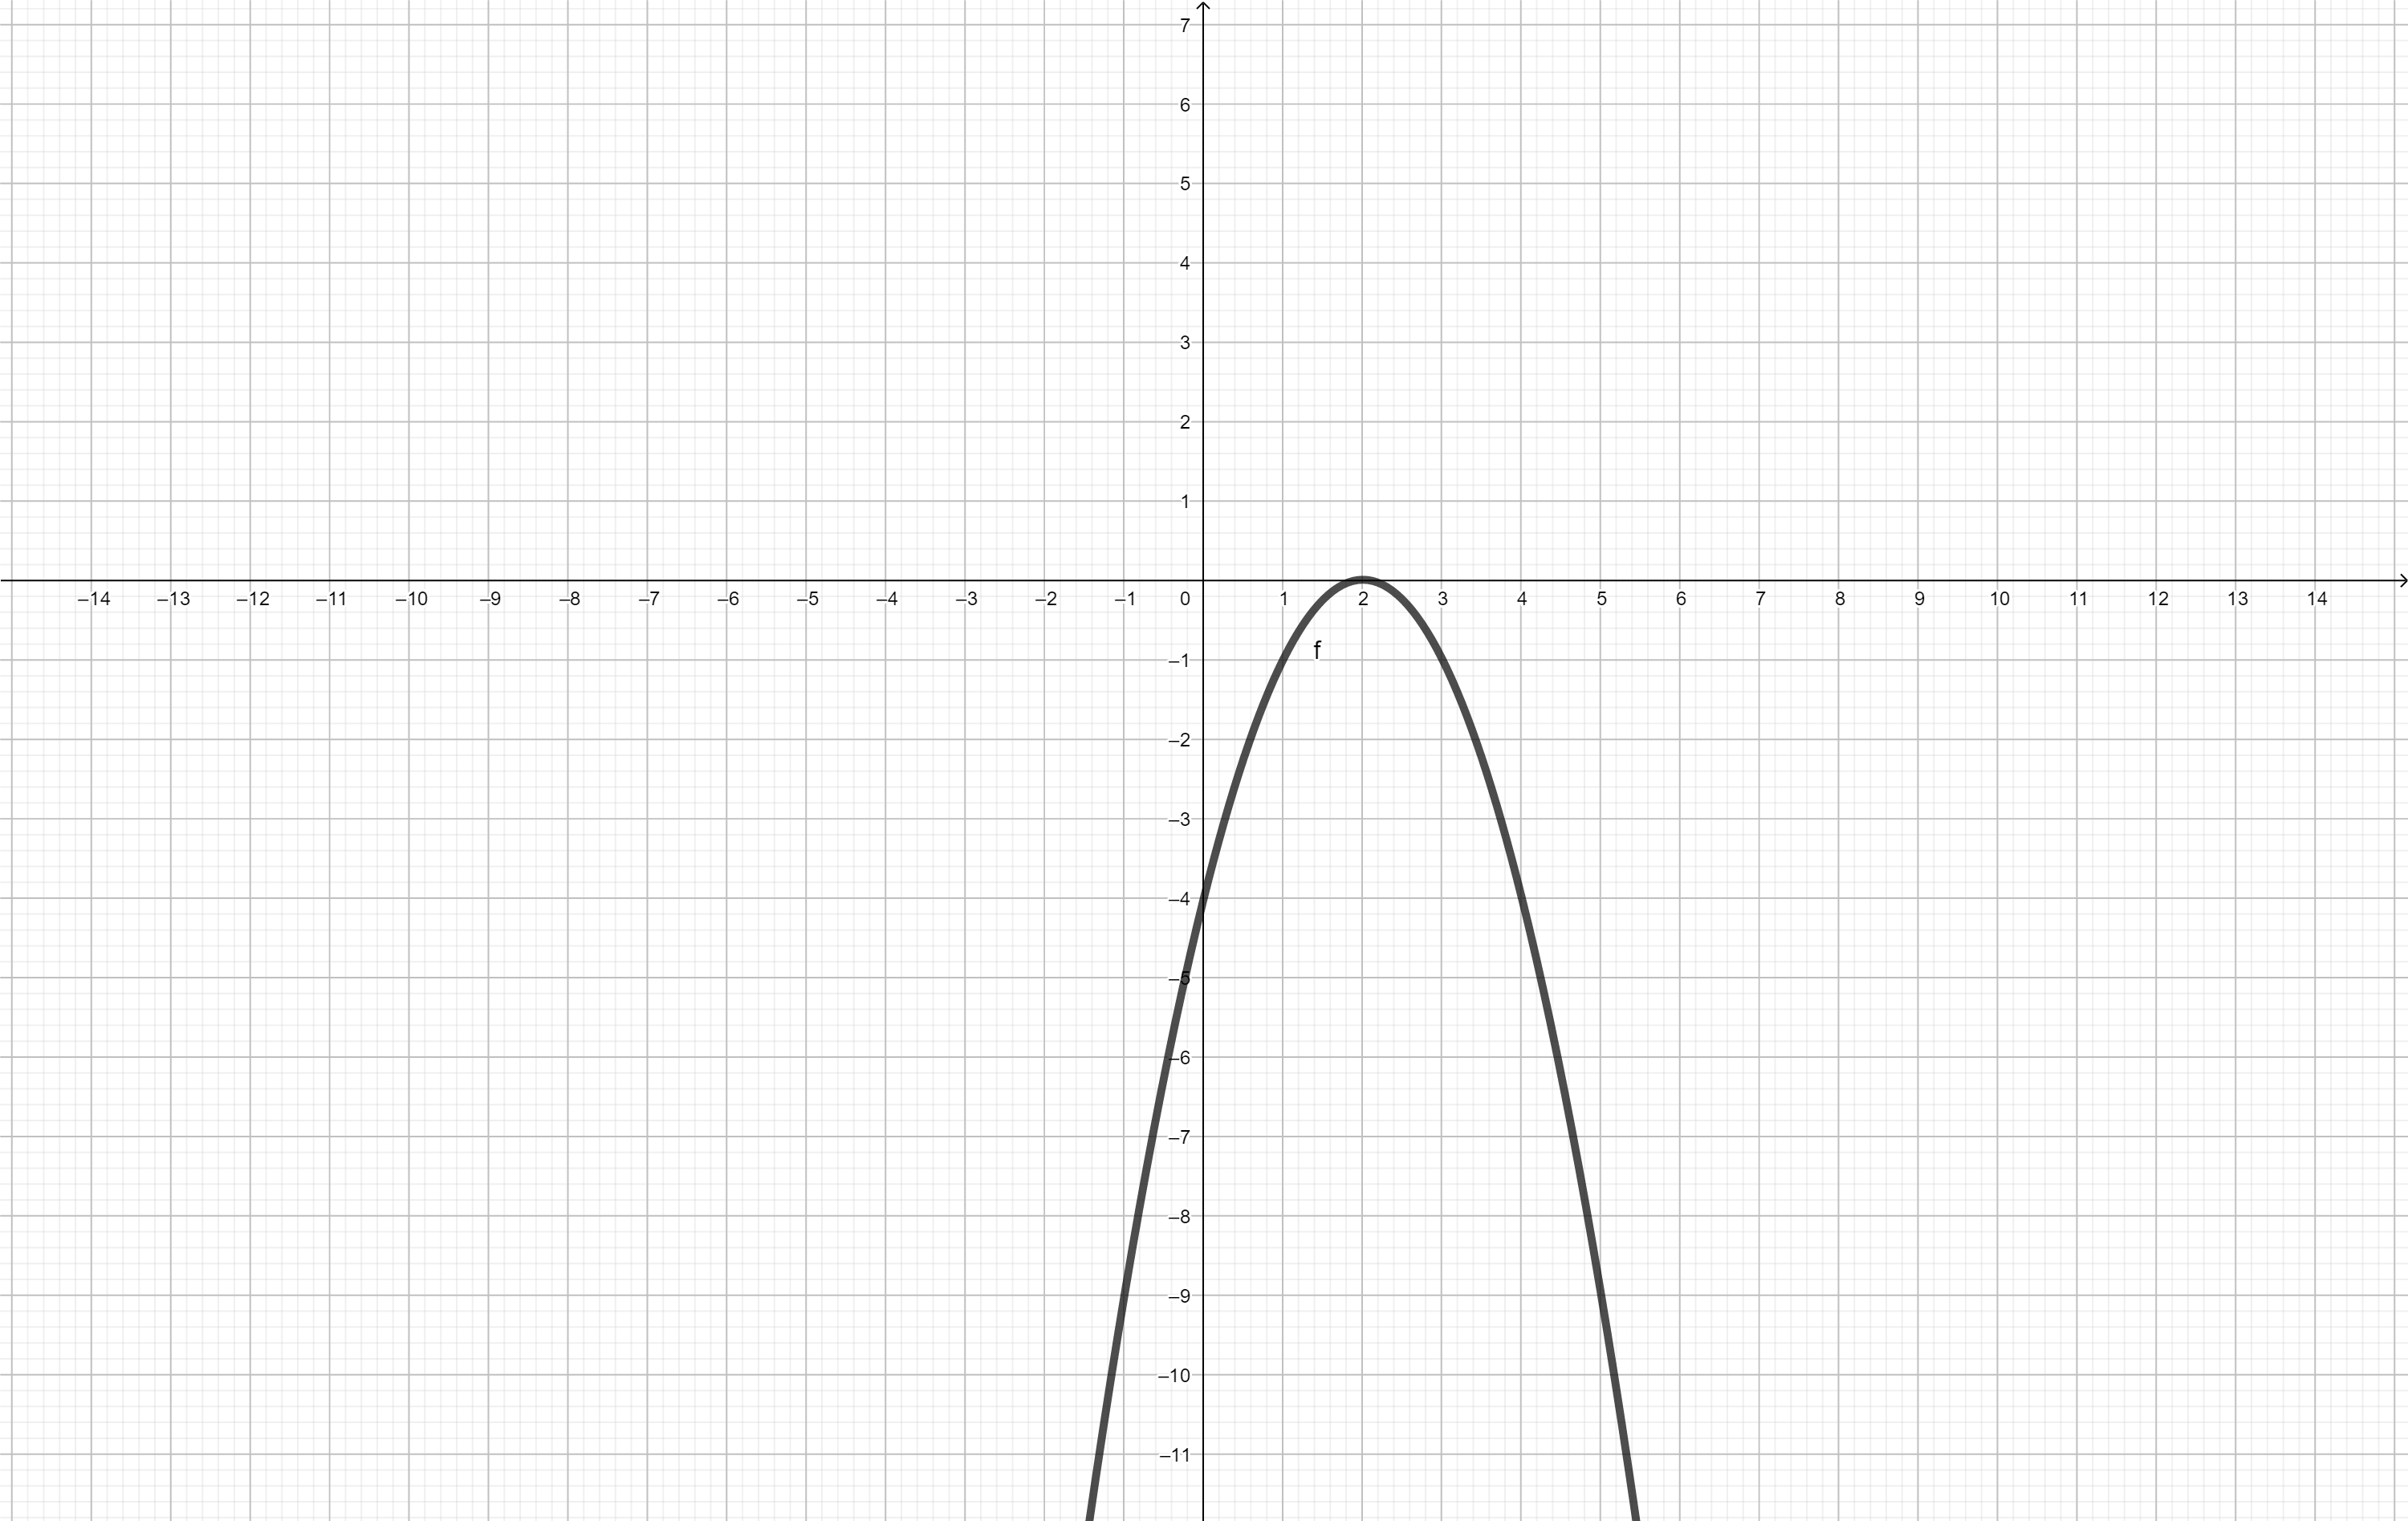
\includegraphics[width=4cm]{Bilder/G23}\hfill
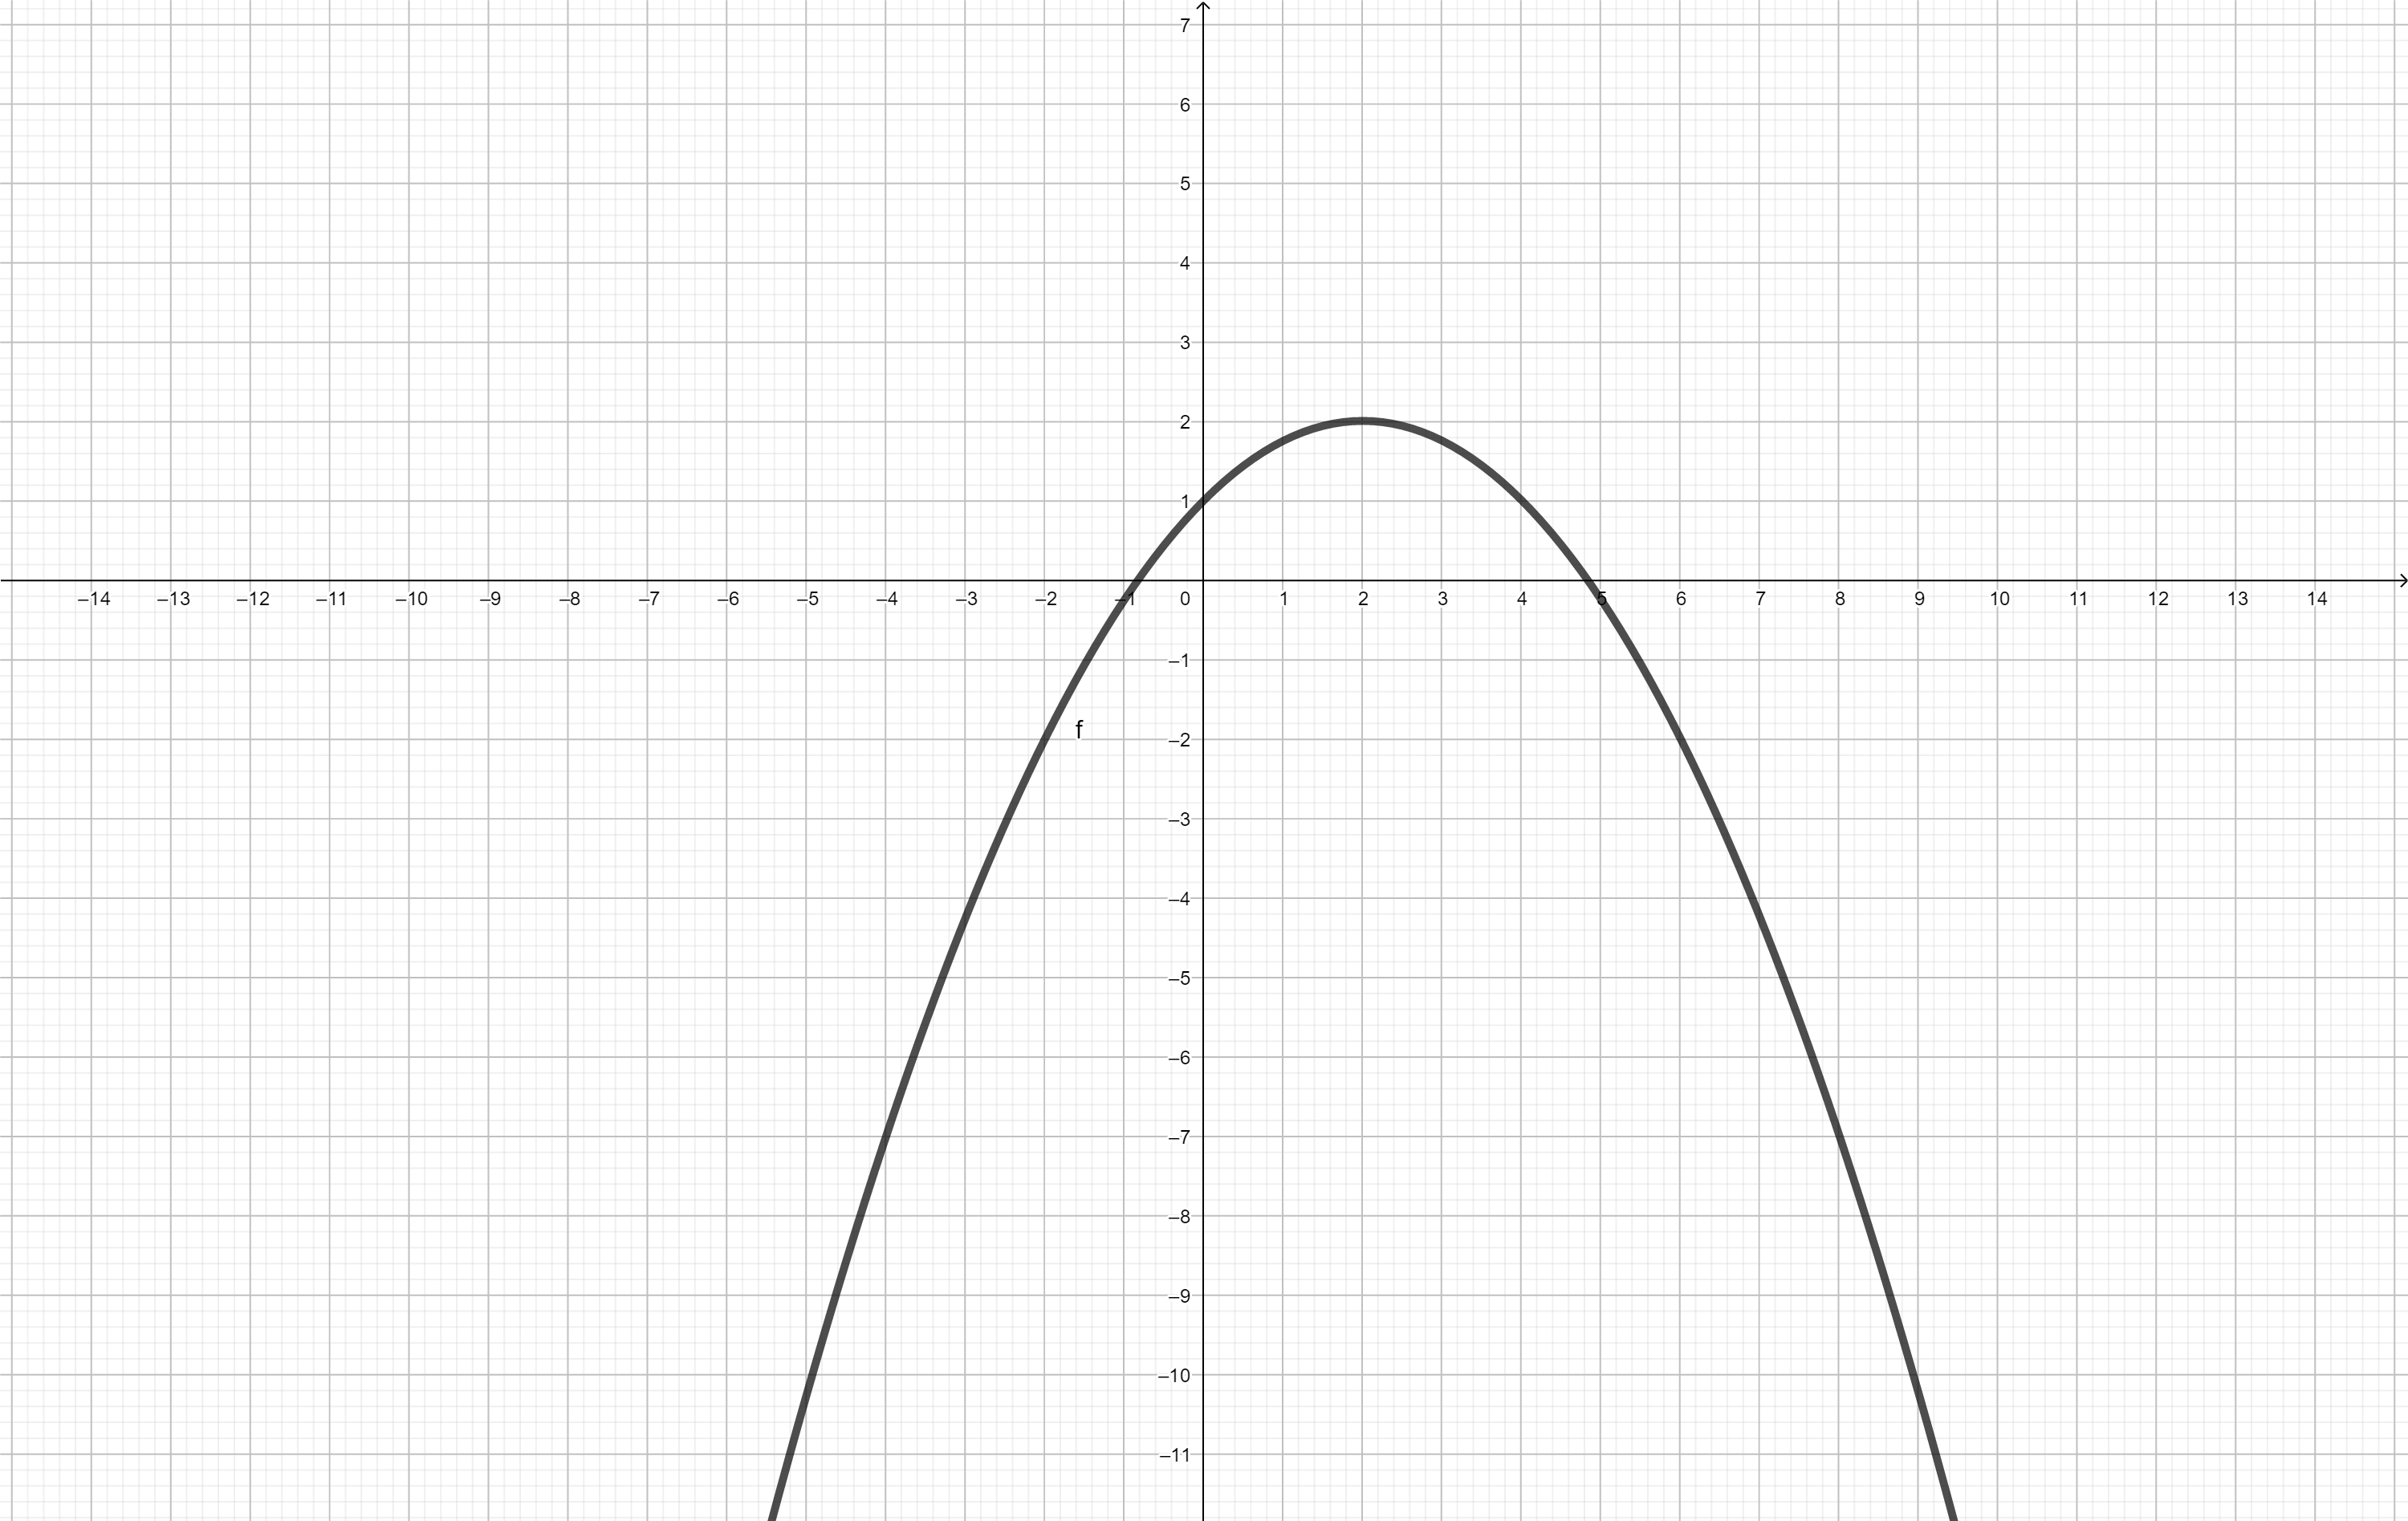
\includegraphics[width=4cm]{Bilder/G24}

\begin{addmargin}[-2cm]{0pt}
Nullstellen:

$x\rightarrow\infty:$

$x\rightarrow-\infty:$
\end{addmargin}

\paragraph{Grad 3:}\textcolor{white}{.}

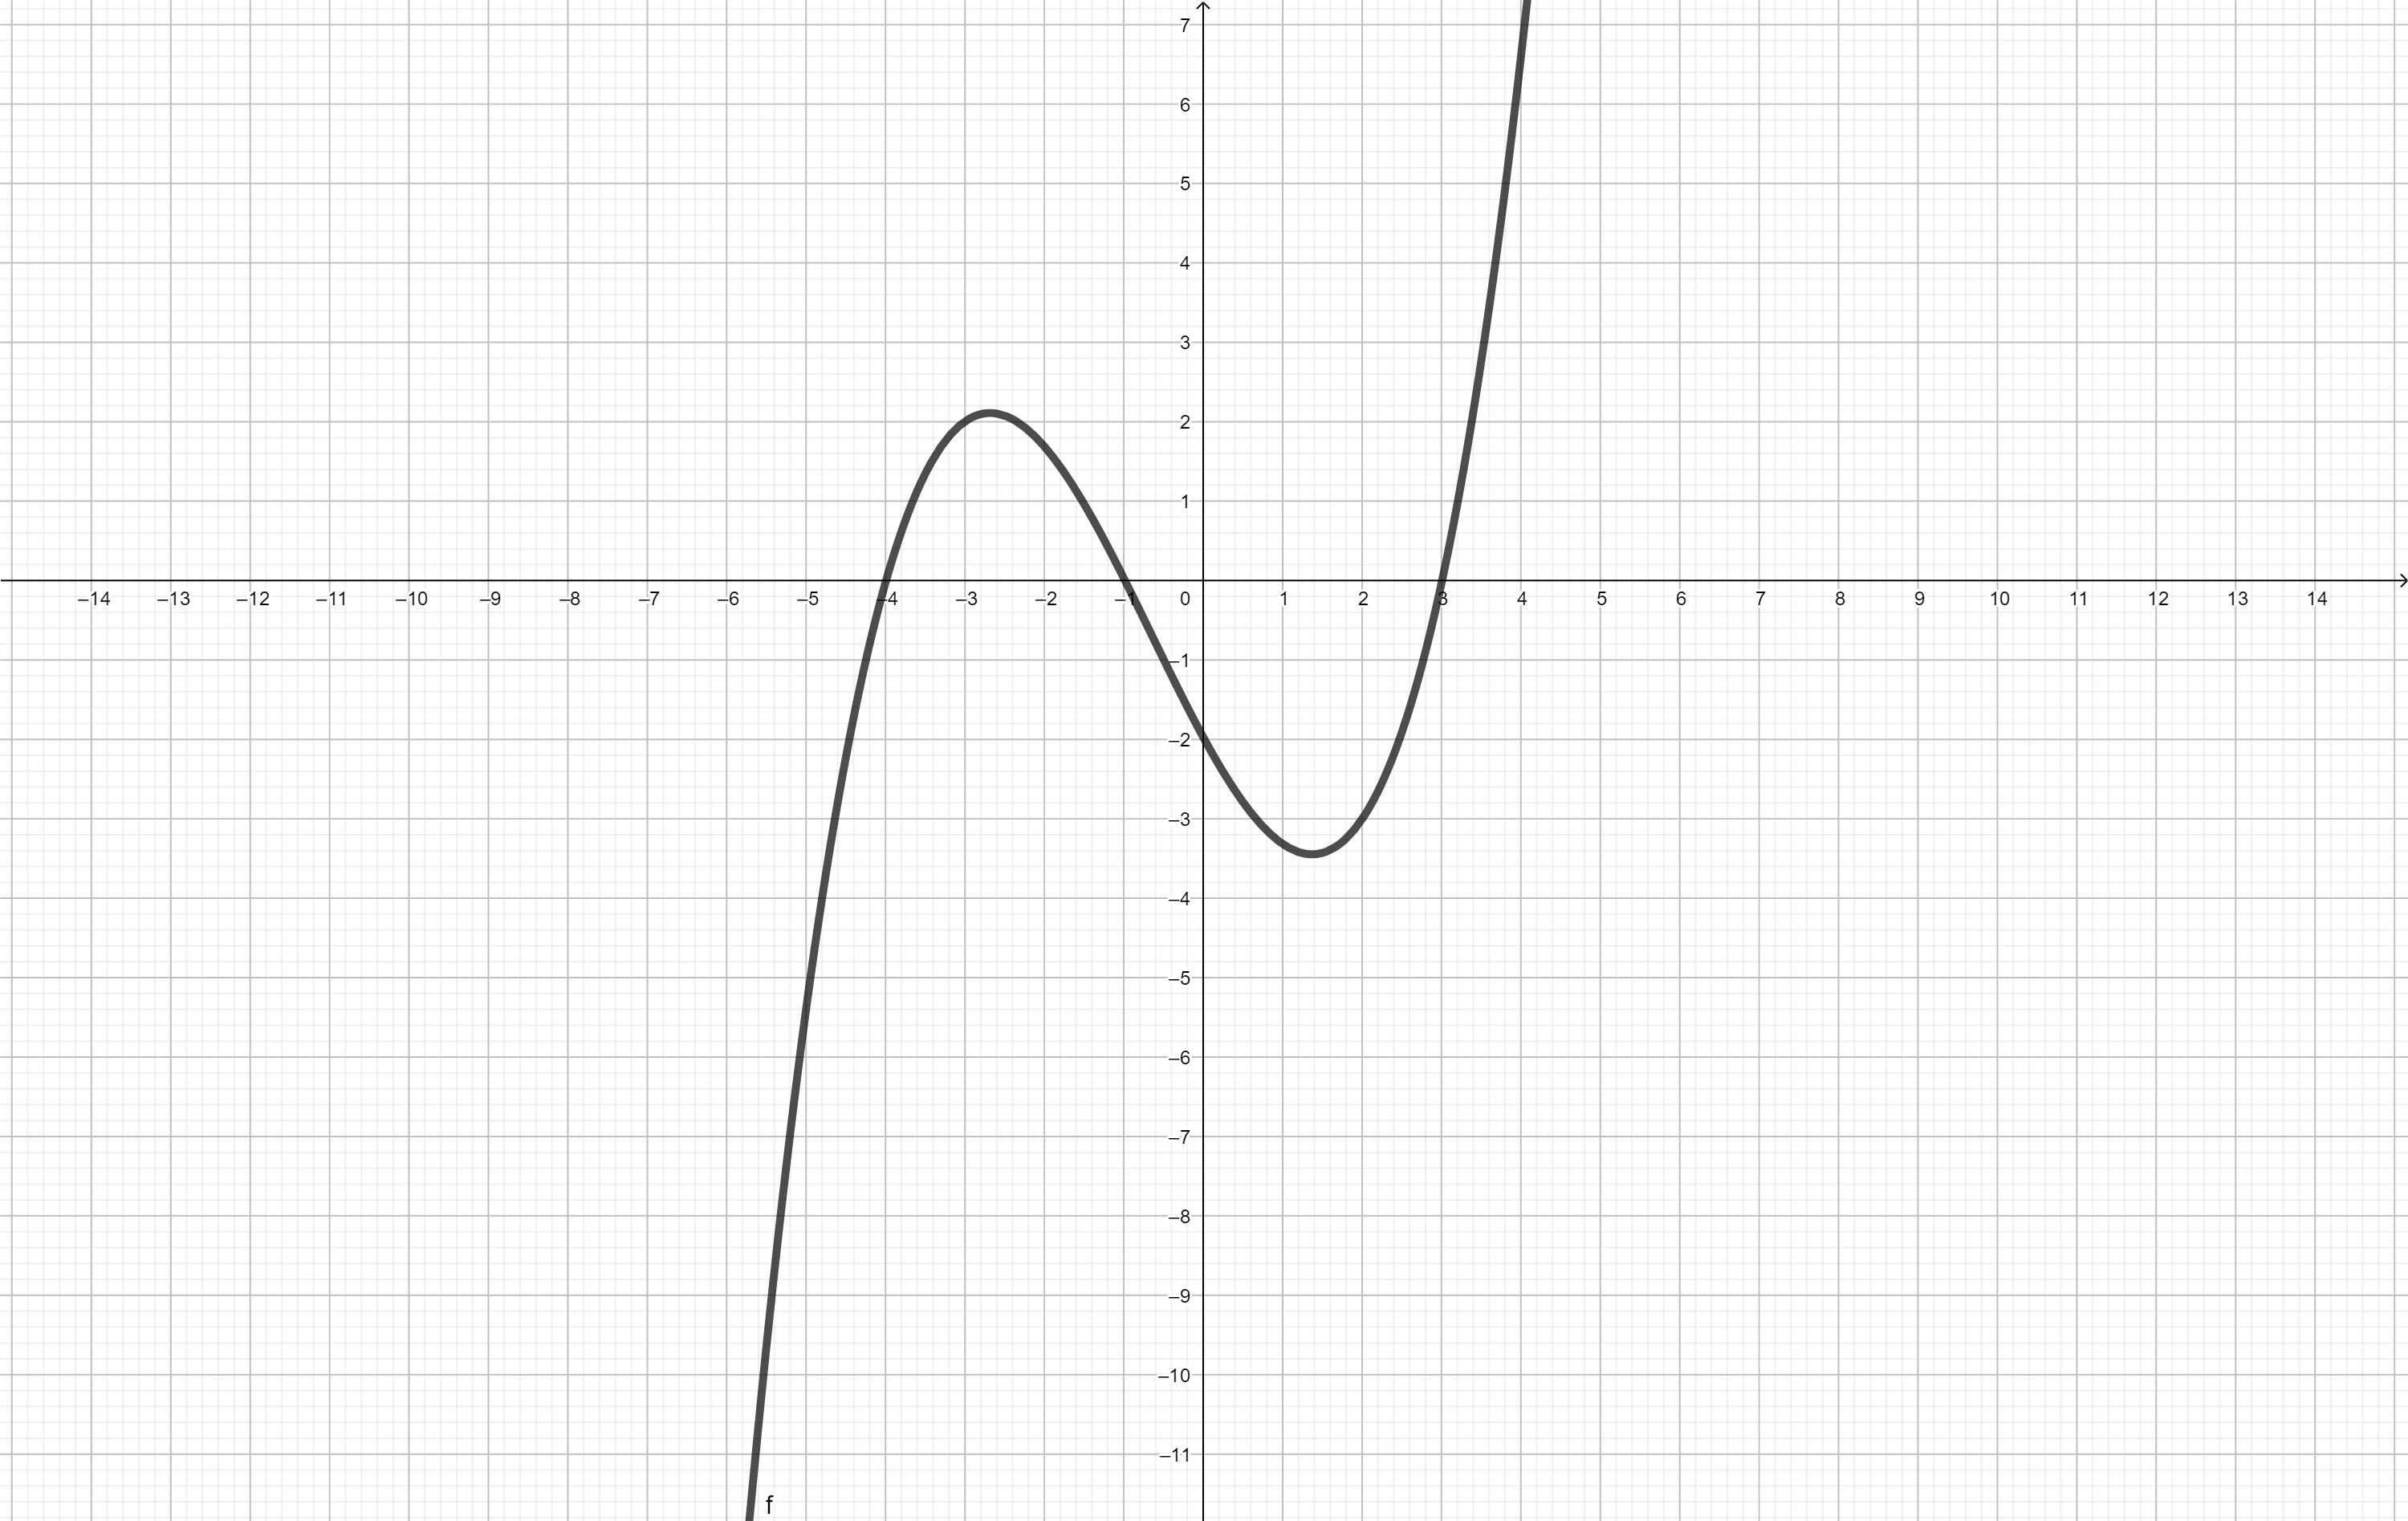
\includegraphics[width=4cm]{Bilder/G31}\hfill
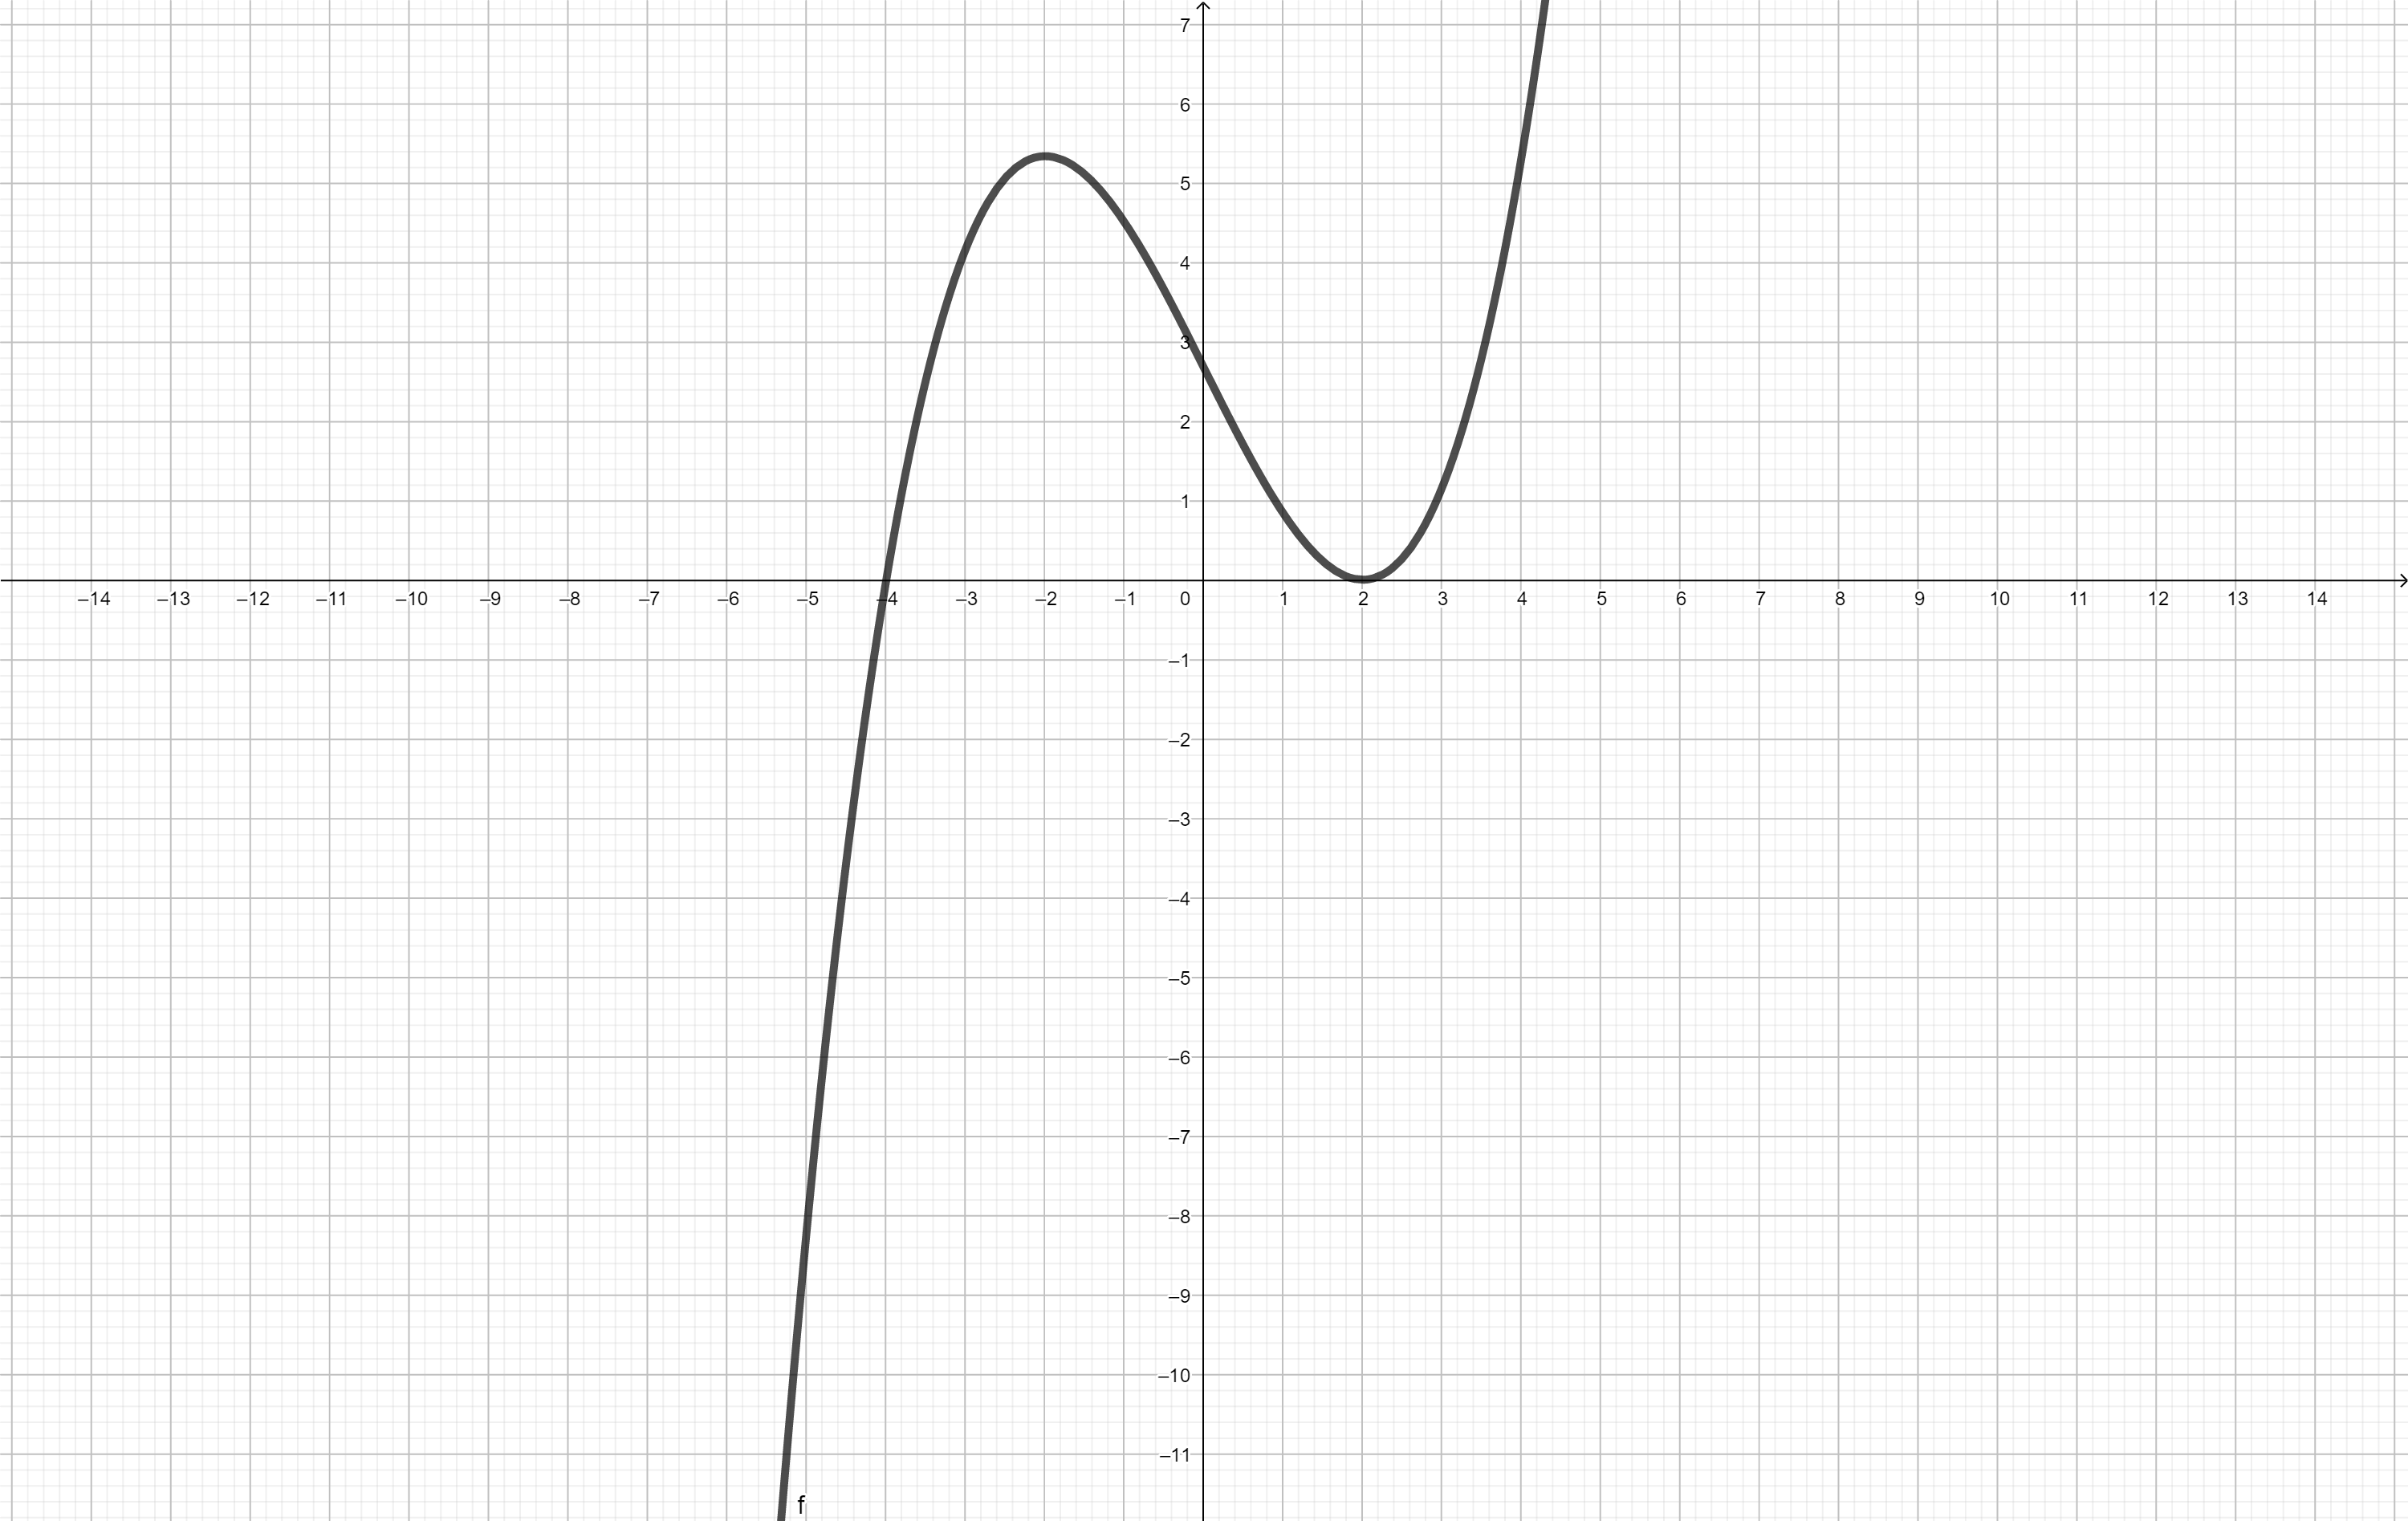
\includegraphics[width=4cm]{Bilder/G32}\hfill
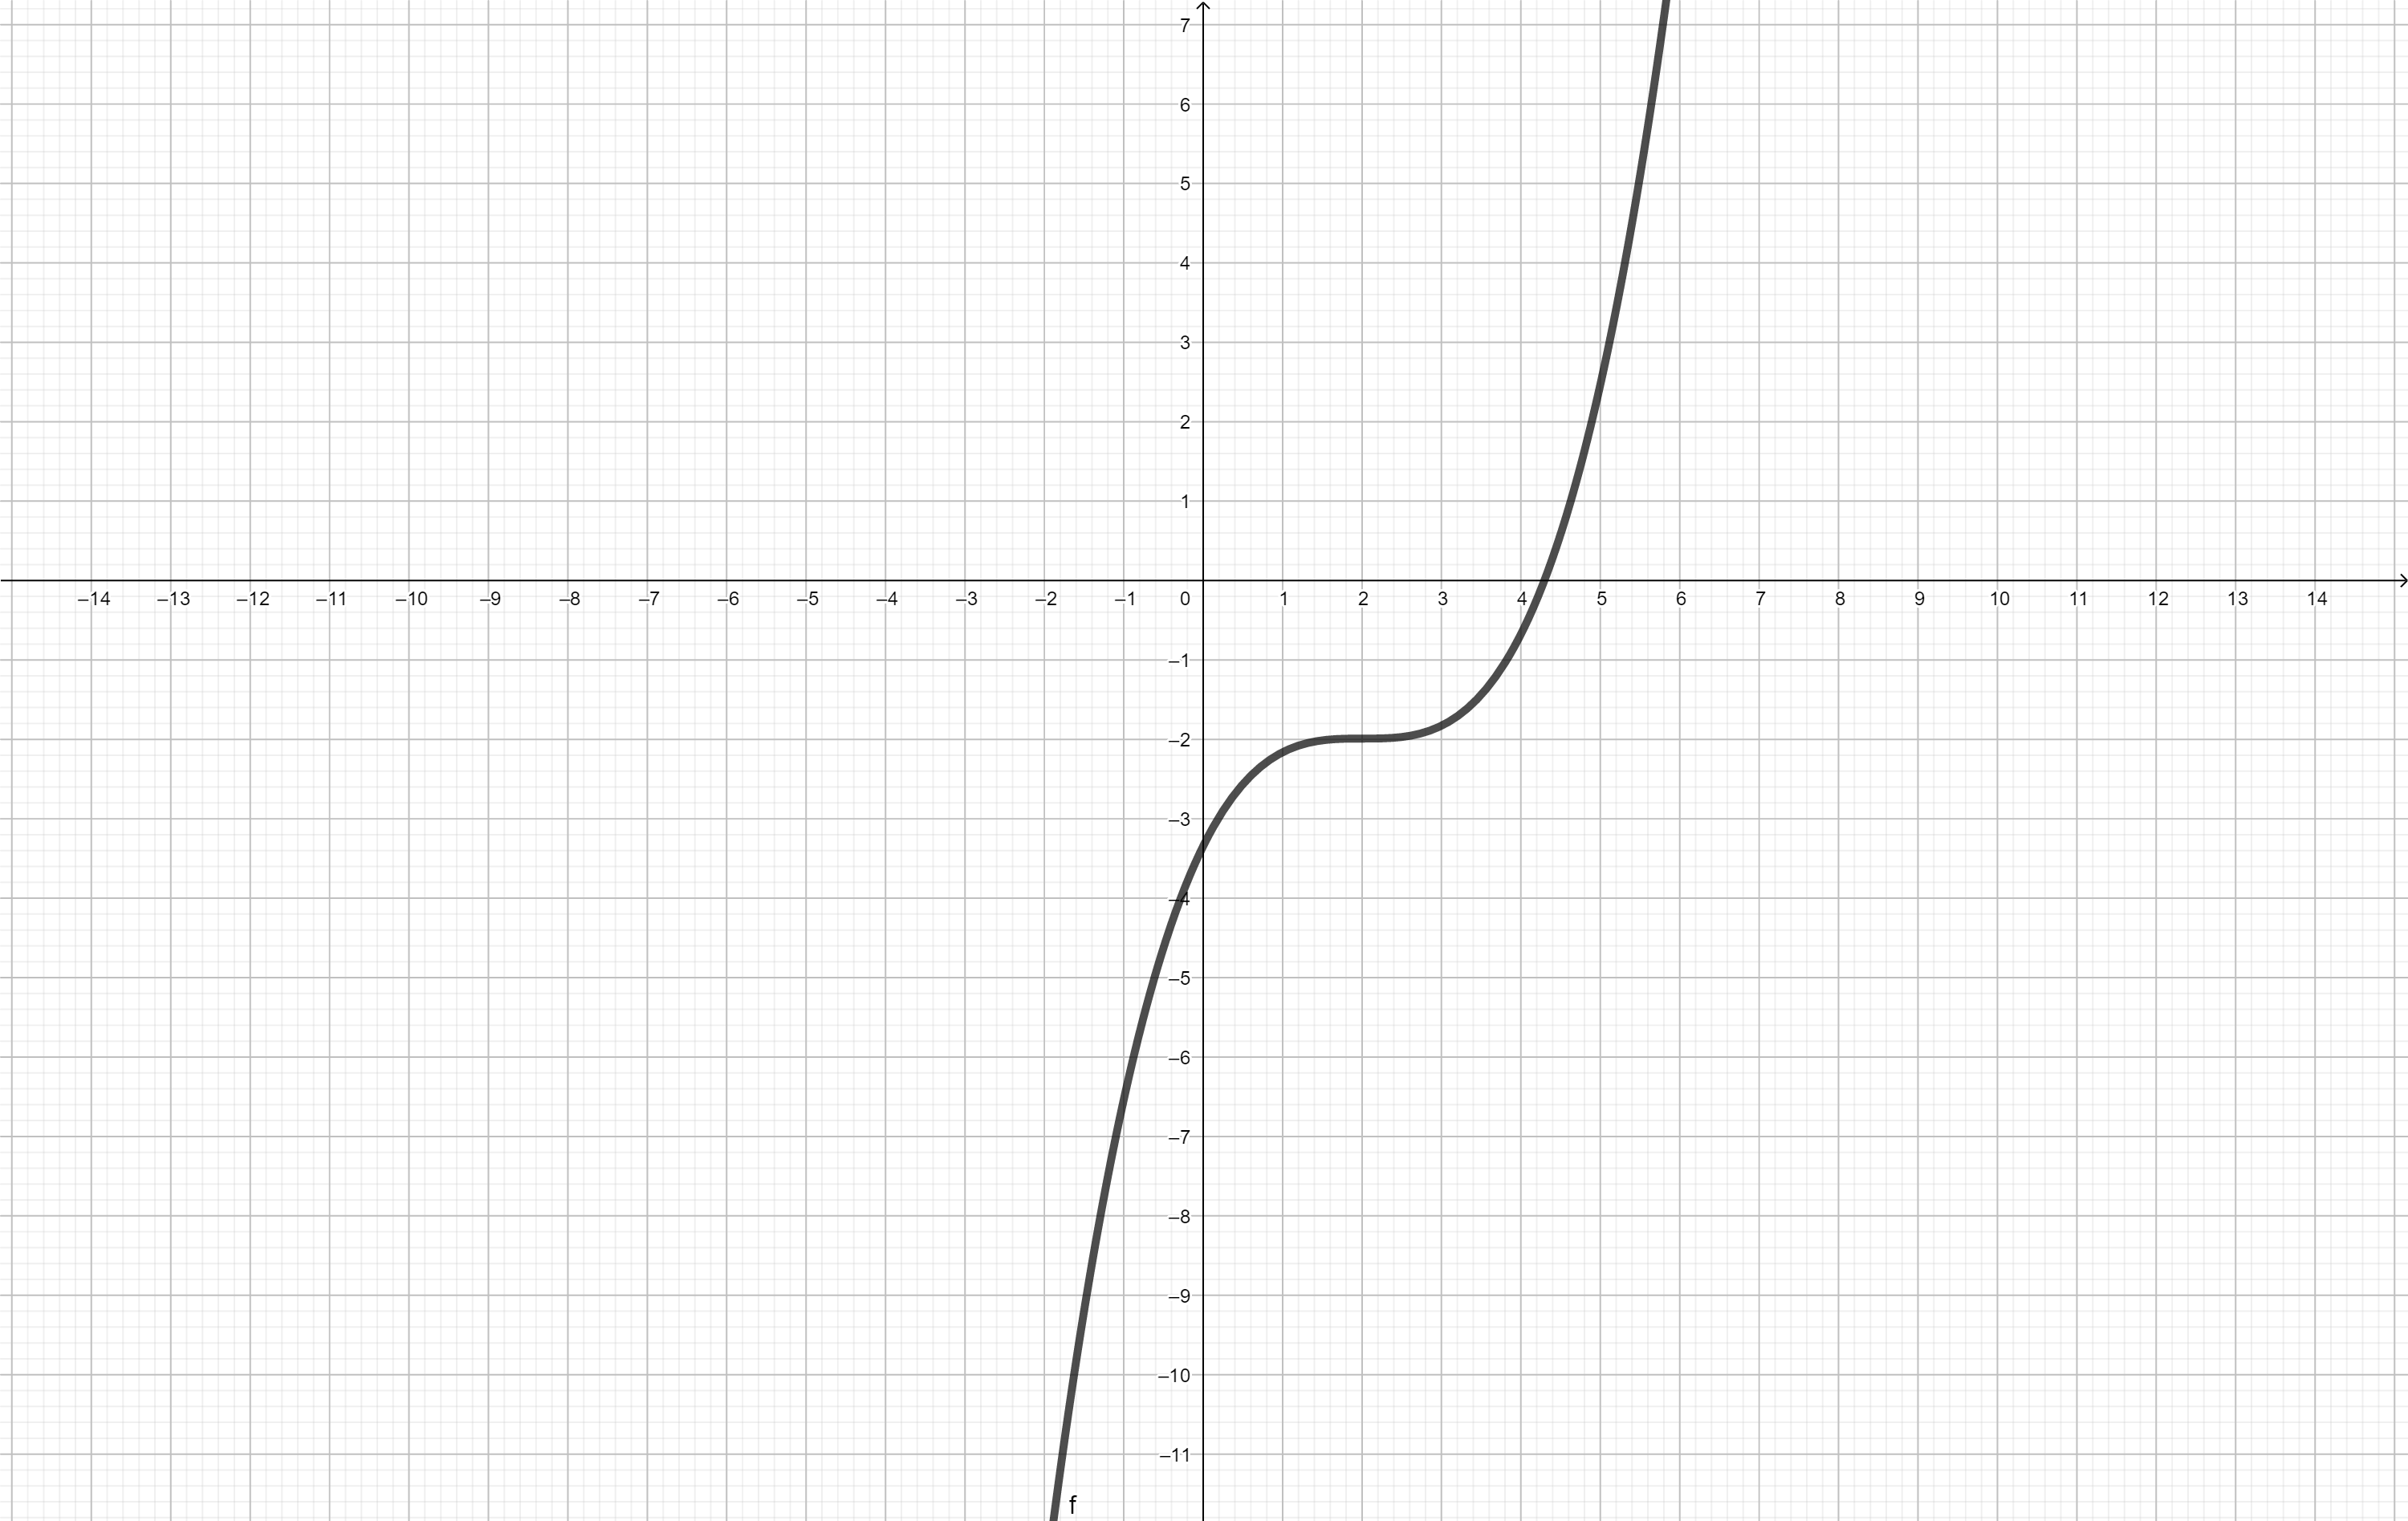
\includegraphics[width=4cm]{Bilder/G33}\hfill
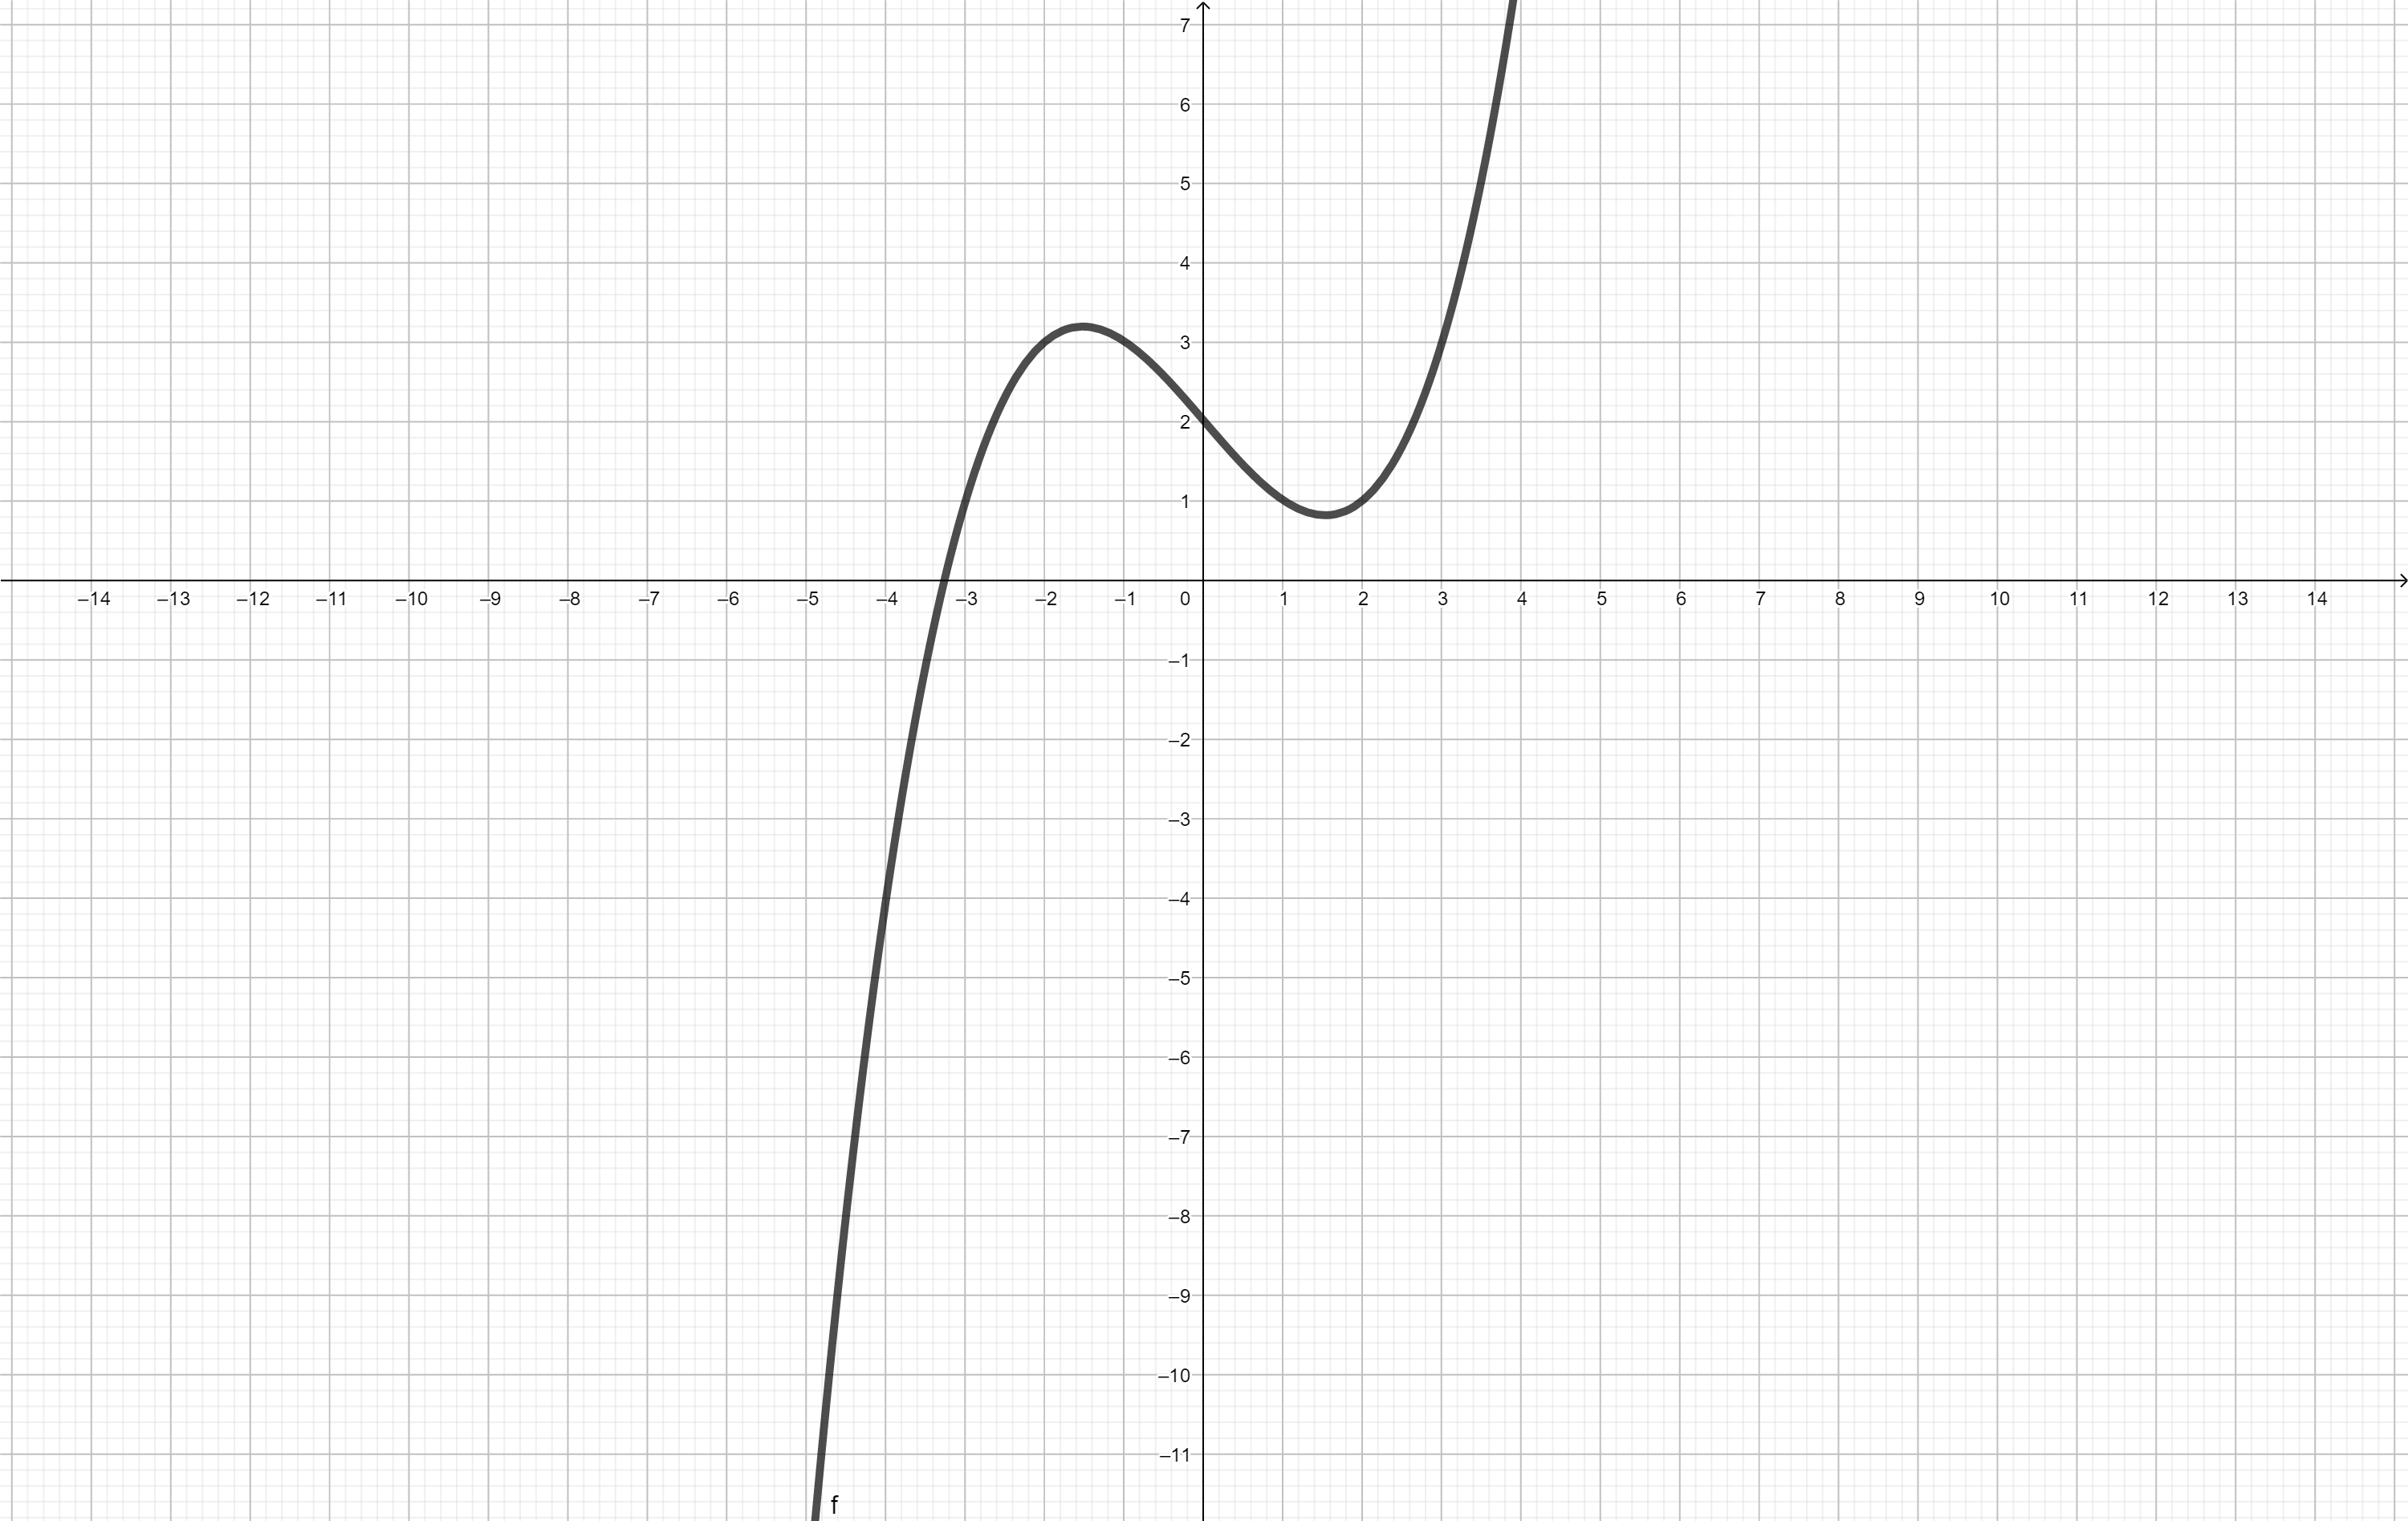
\includegraphics[width=4cm]{Bilder/G34}

\begin{addmargin}[-2cm]{0pt}
Nullstellen:

$x\rightarrow\infty:$

$x\rightarrow-\infty:$
\end{addmargin}

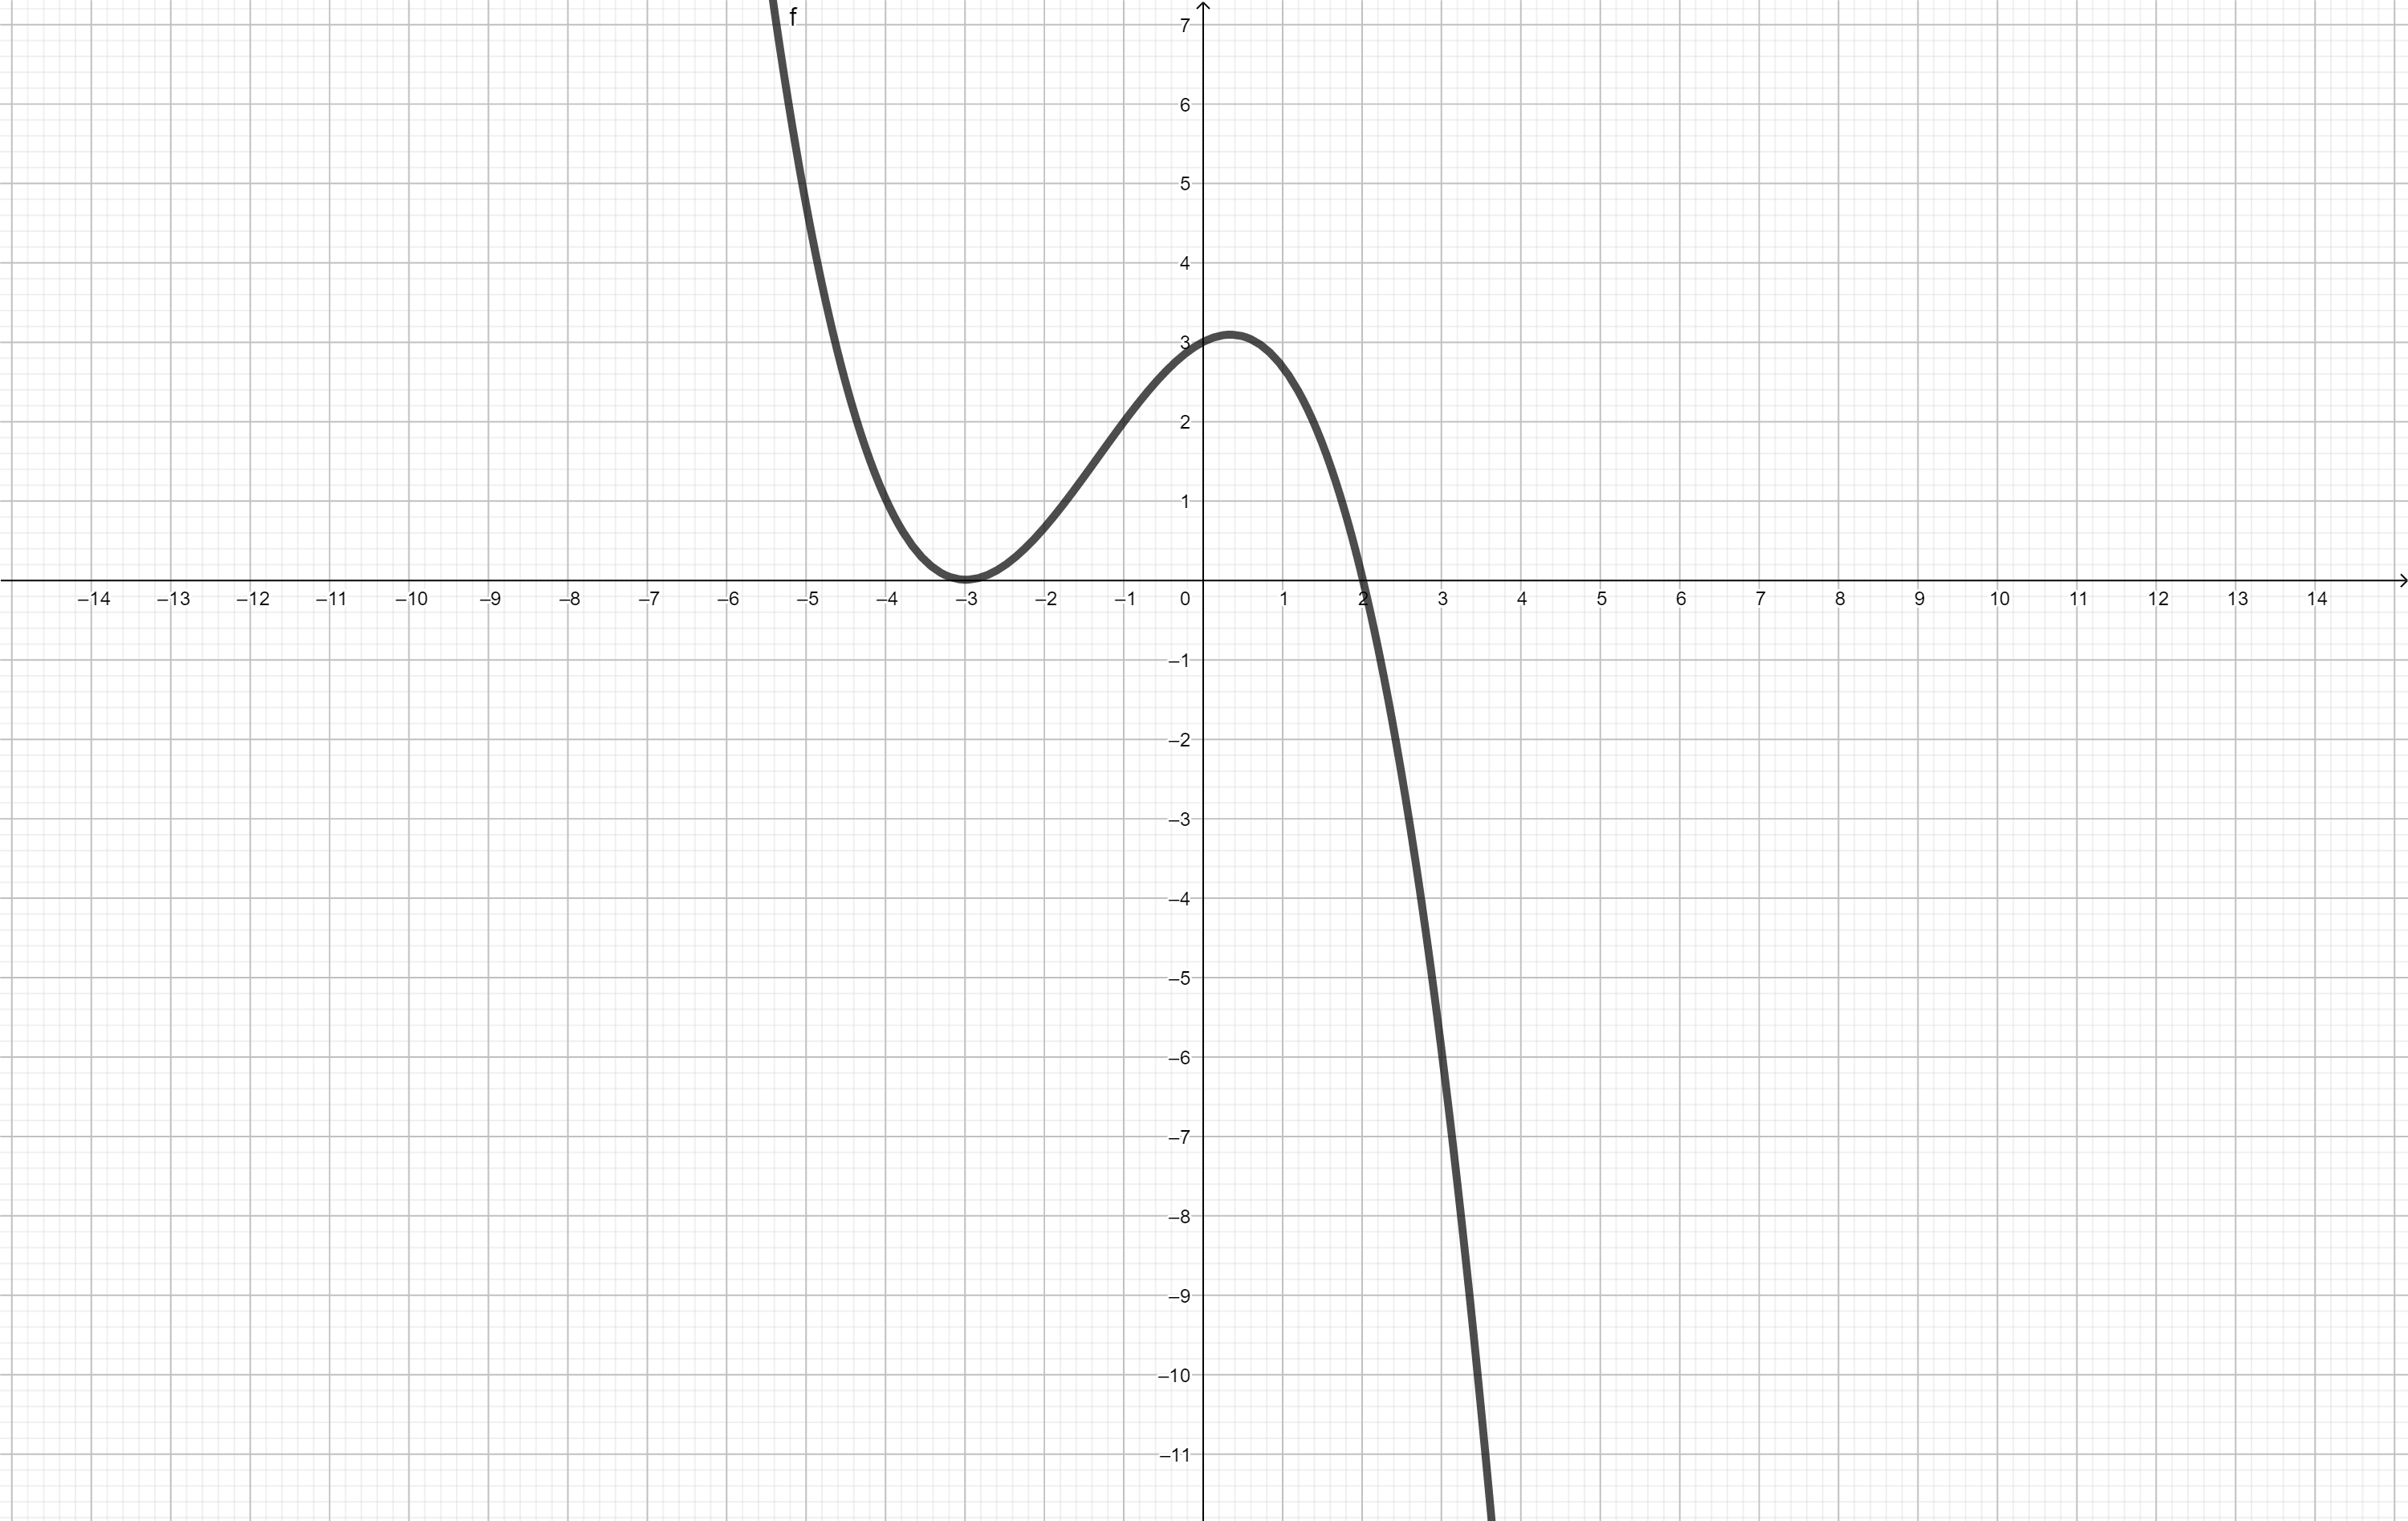
\includegraphics[width=4cm]{Bilder/G35}\hfill
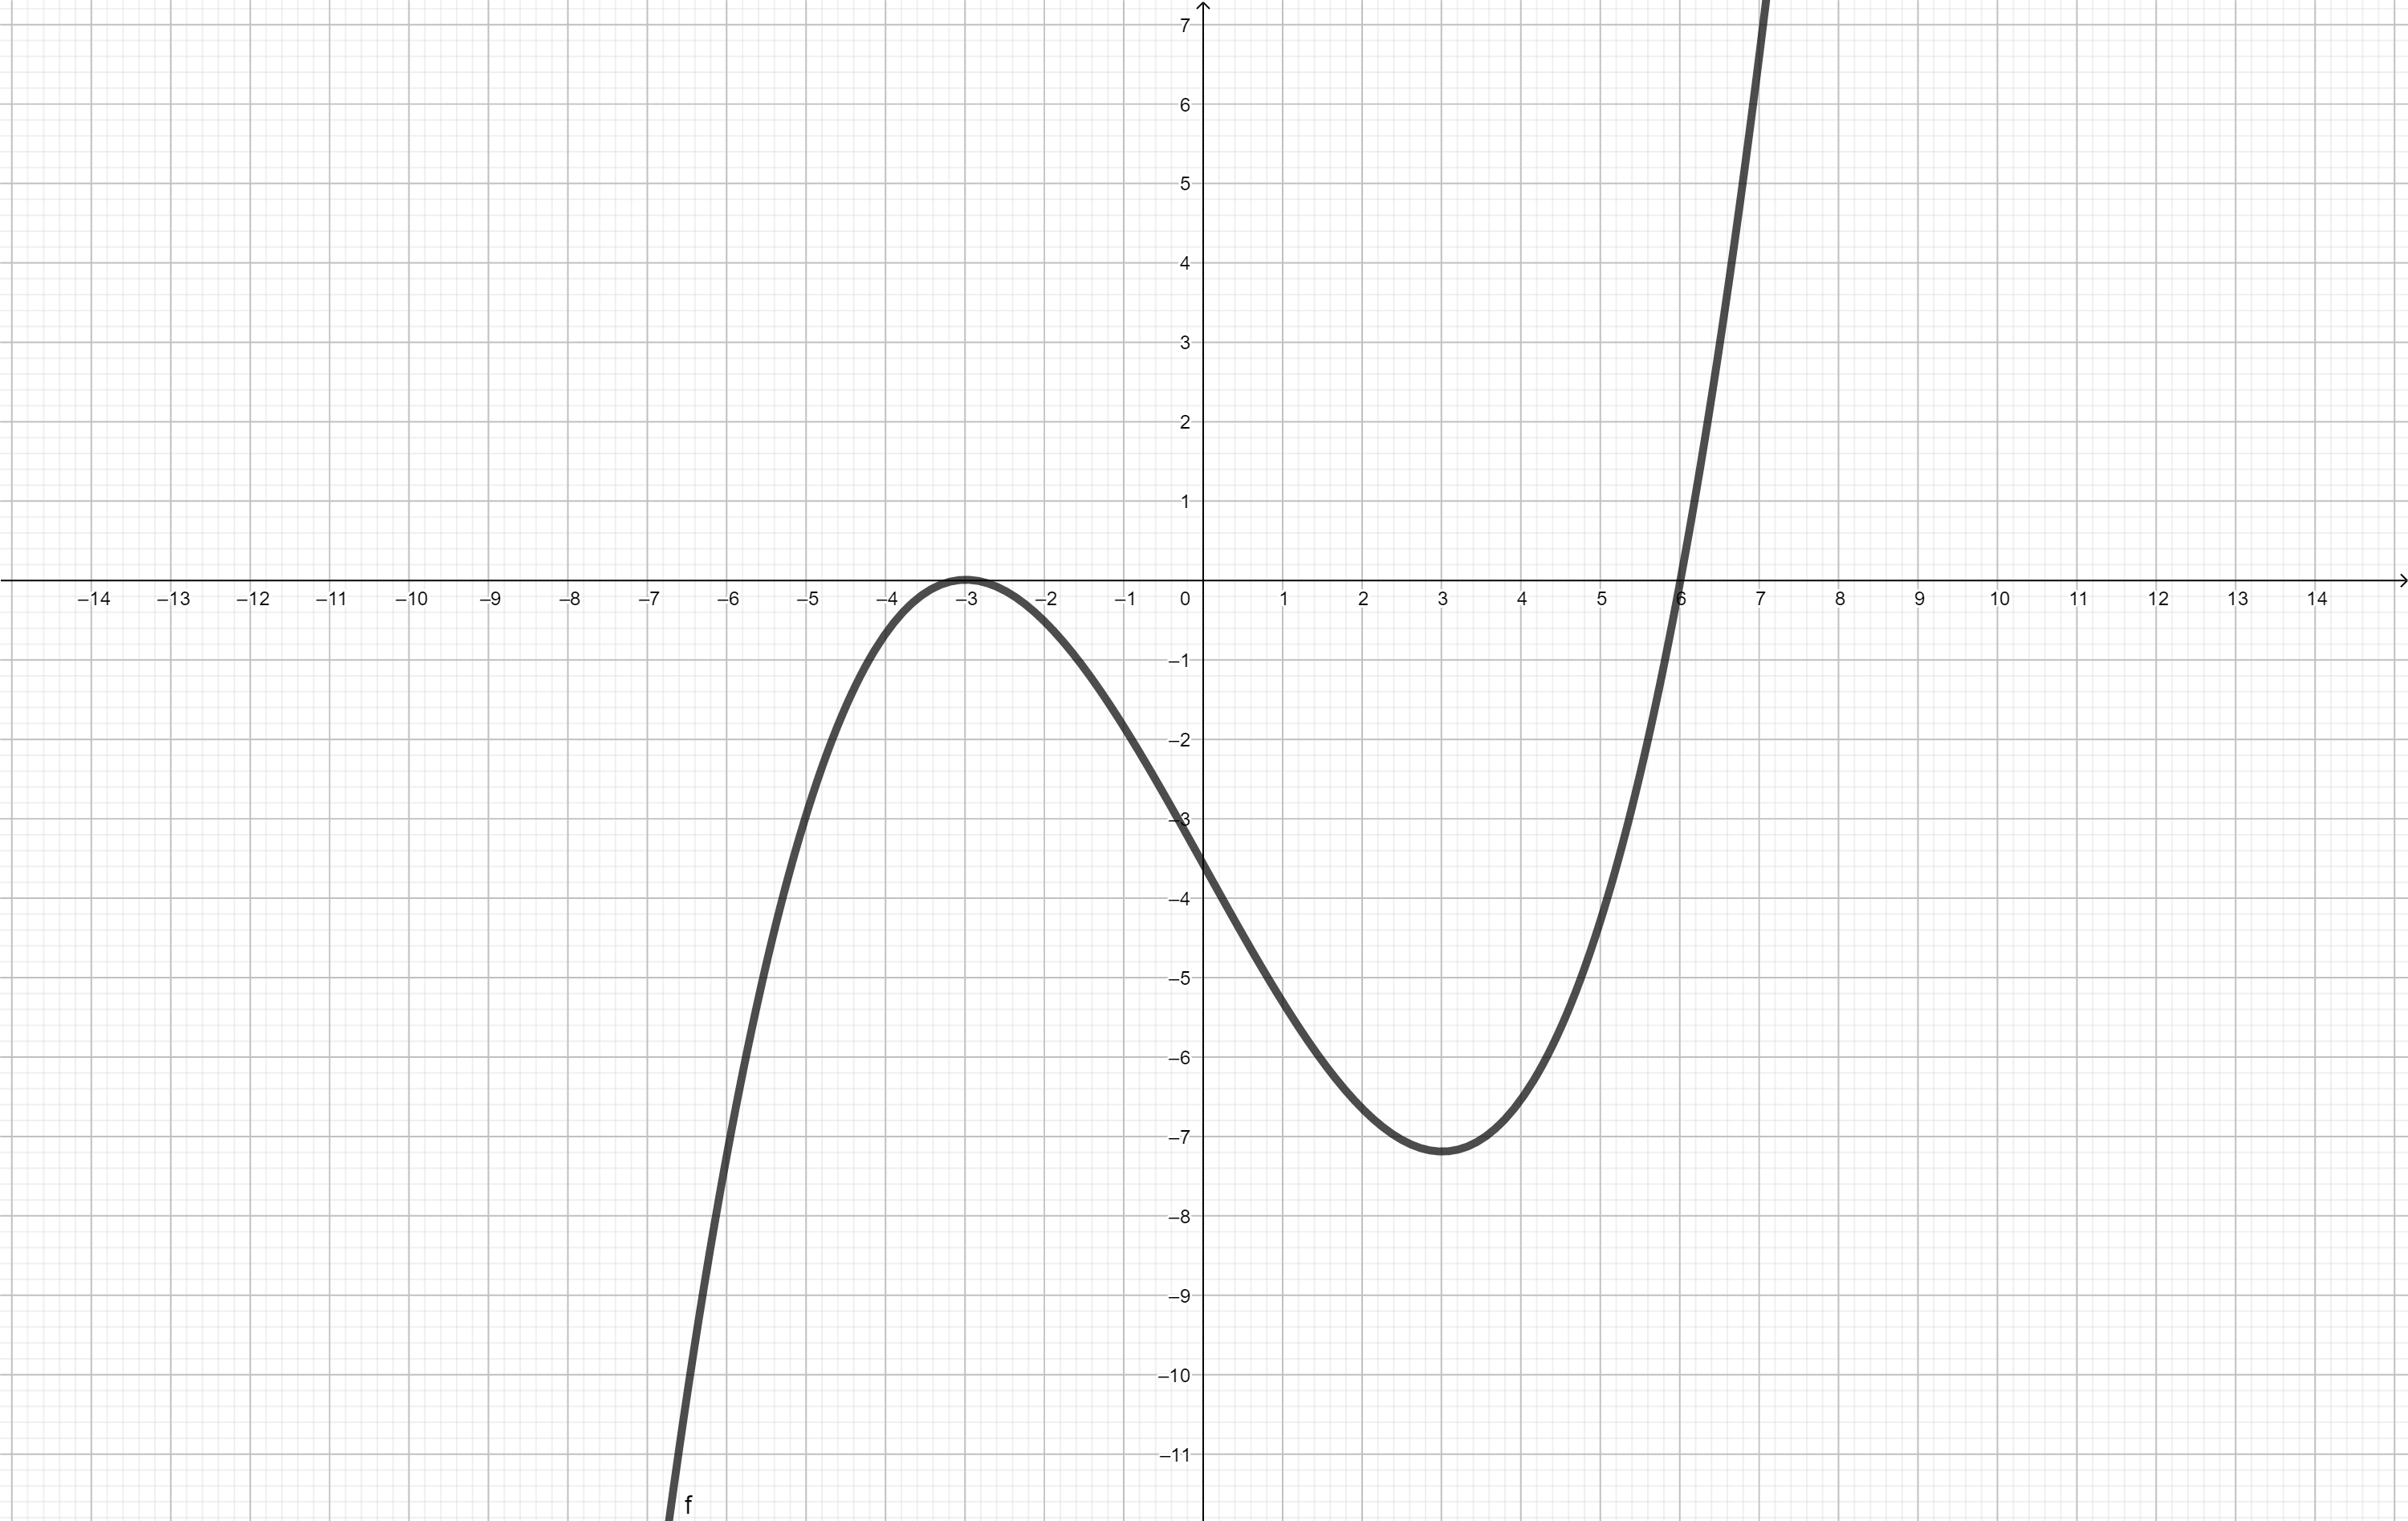
\includegraphics[width=4cm]{Bilder/G36}\hfill
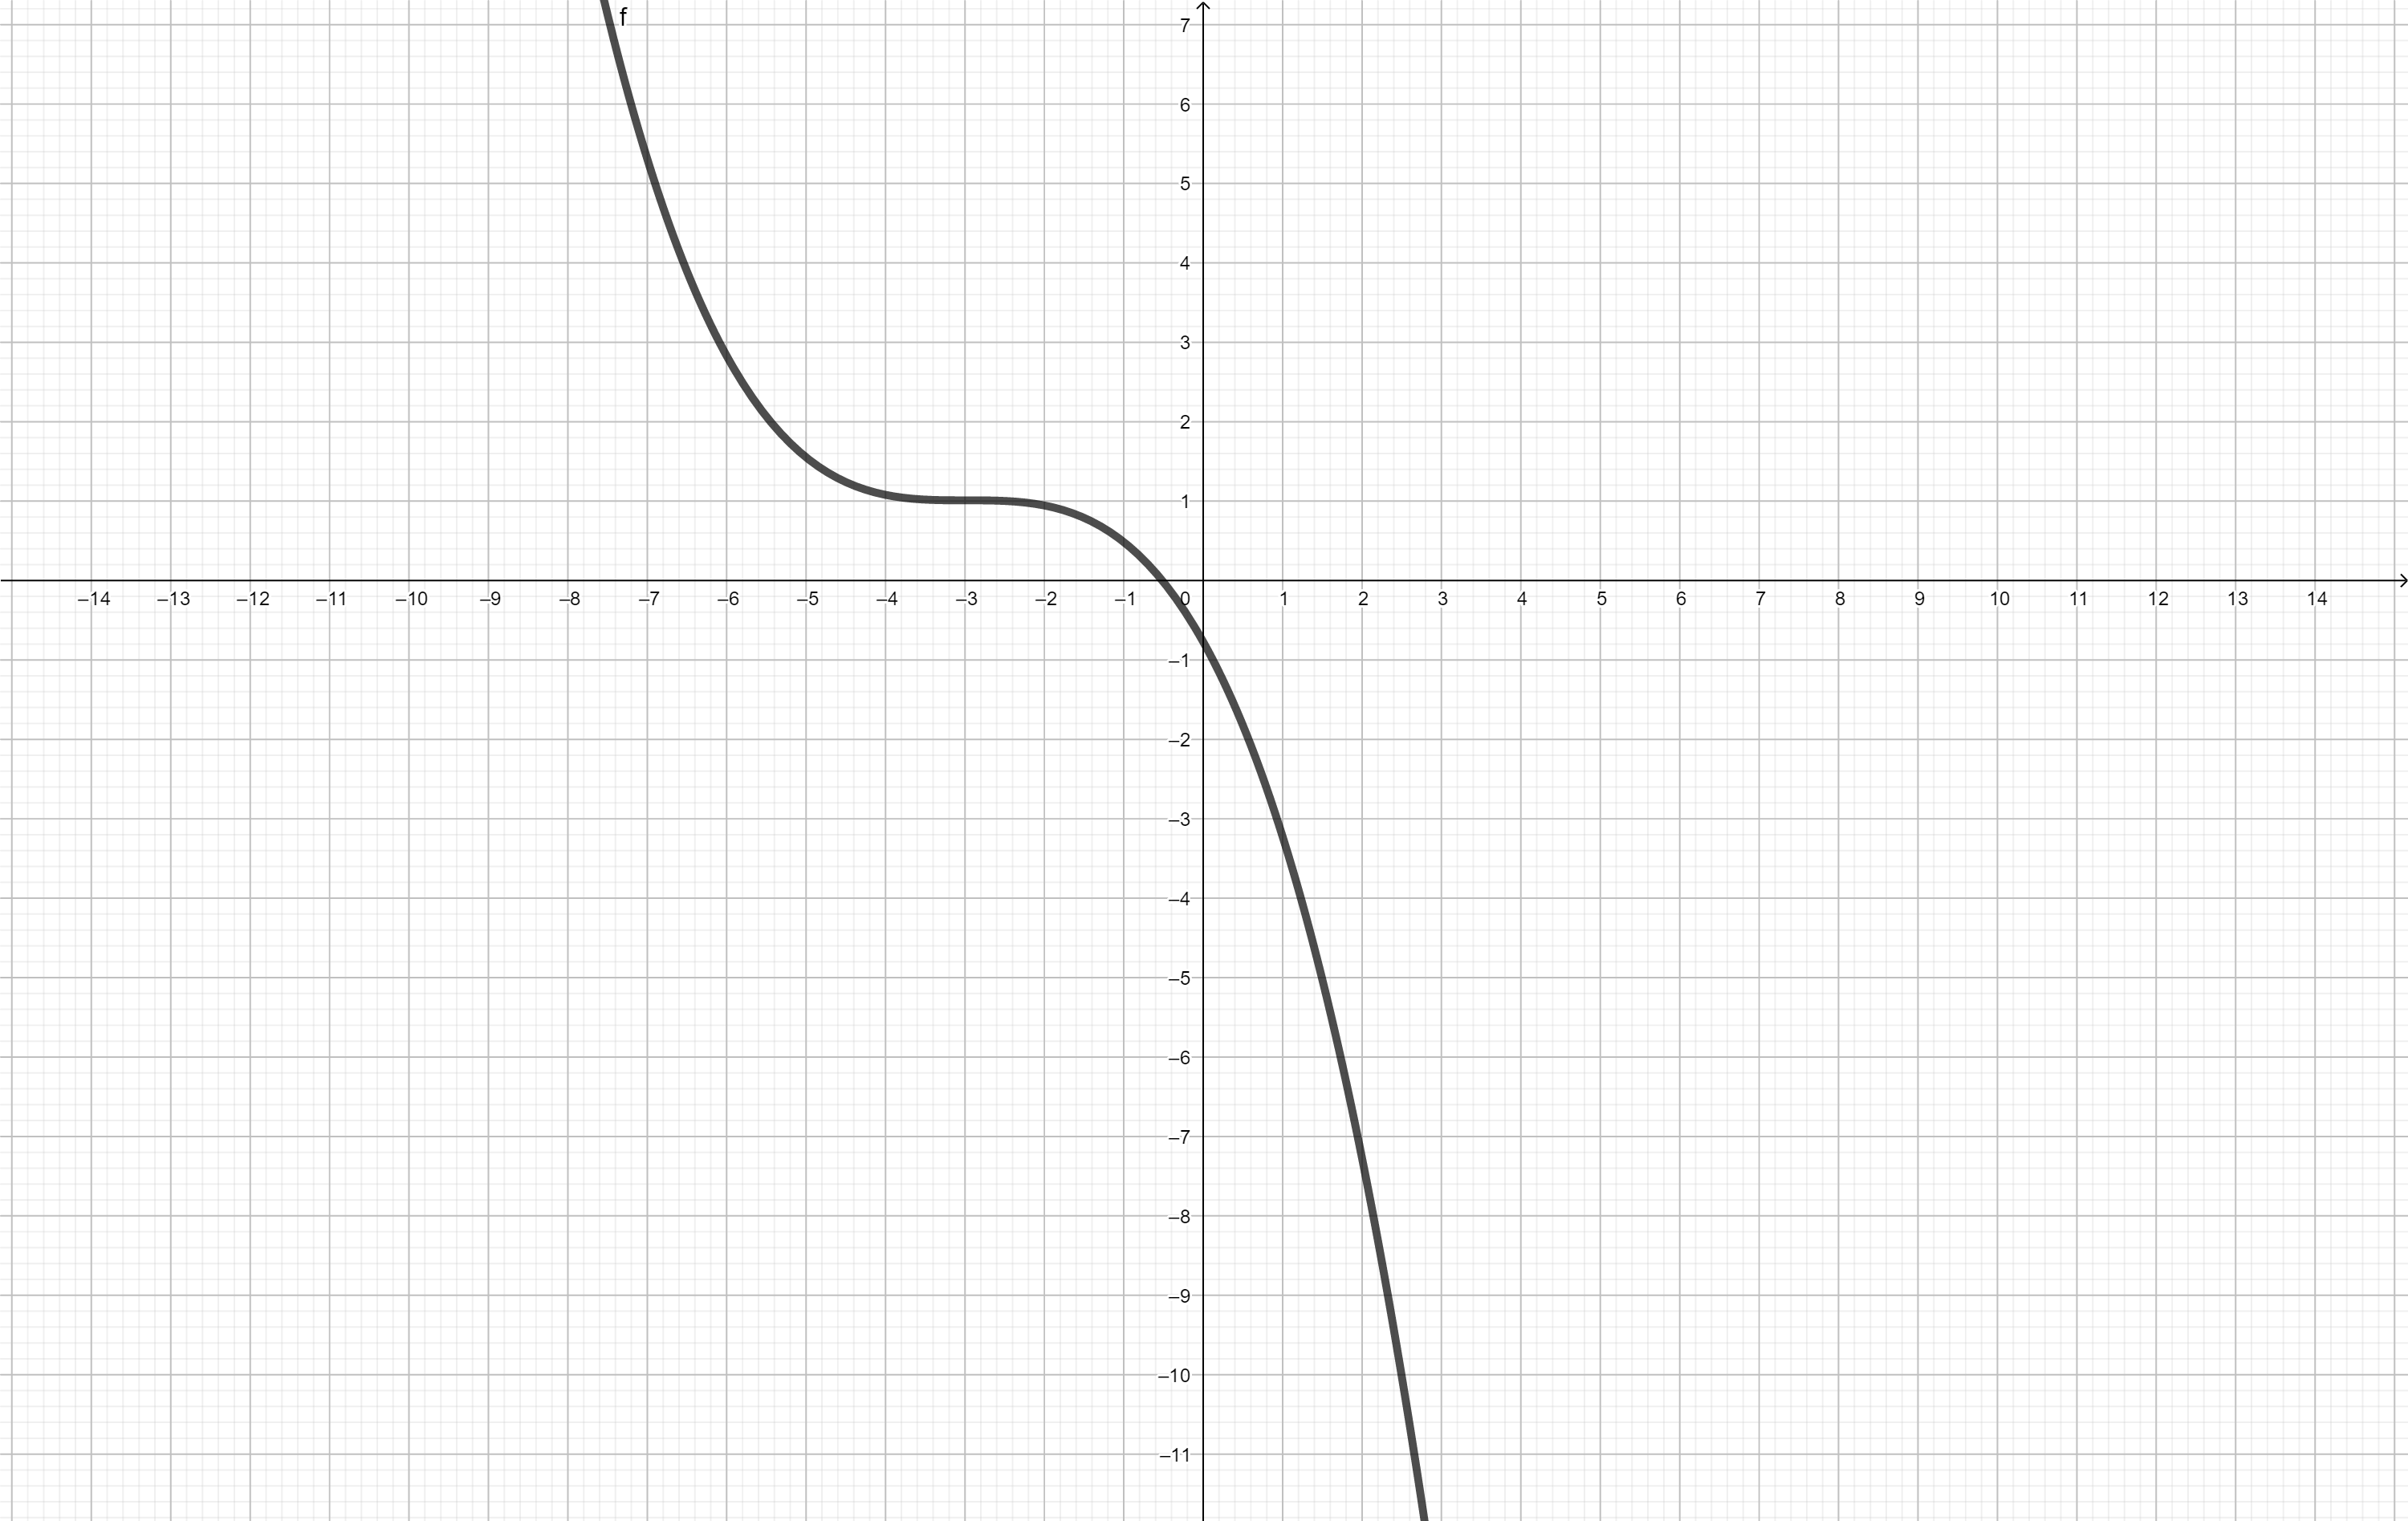
\includegraphics[width=4cm]{Bilder/G37}\hfill
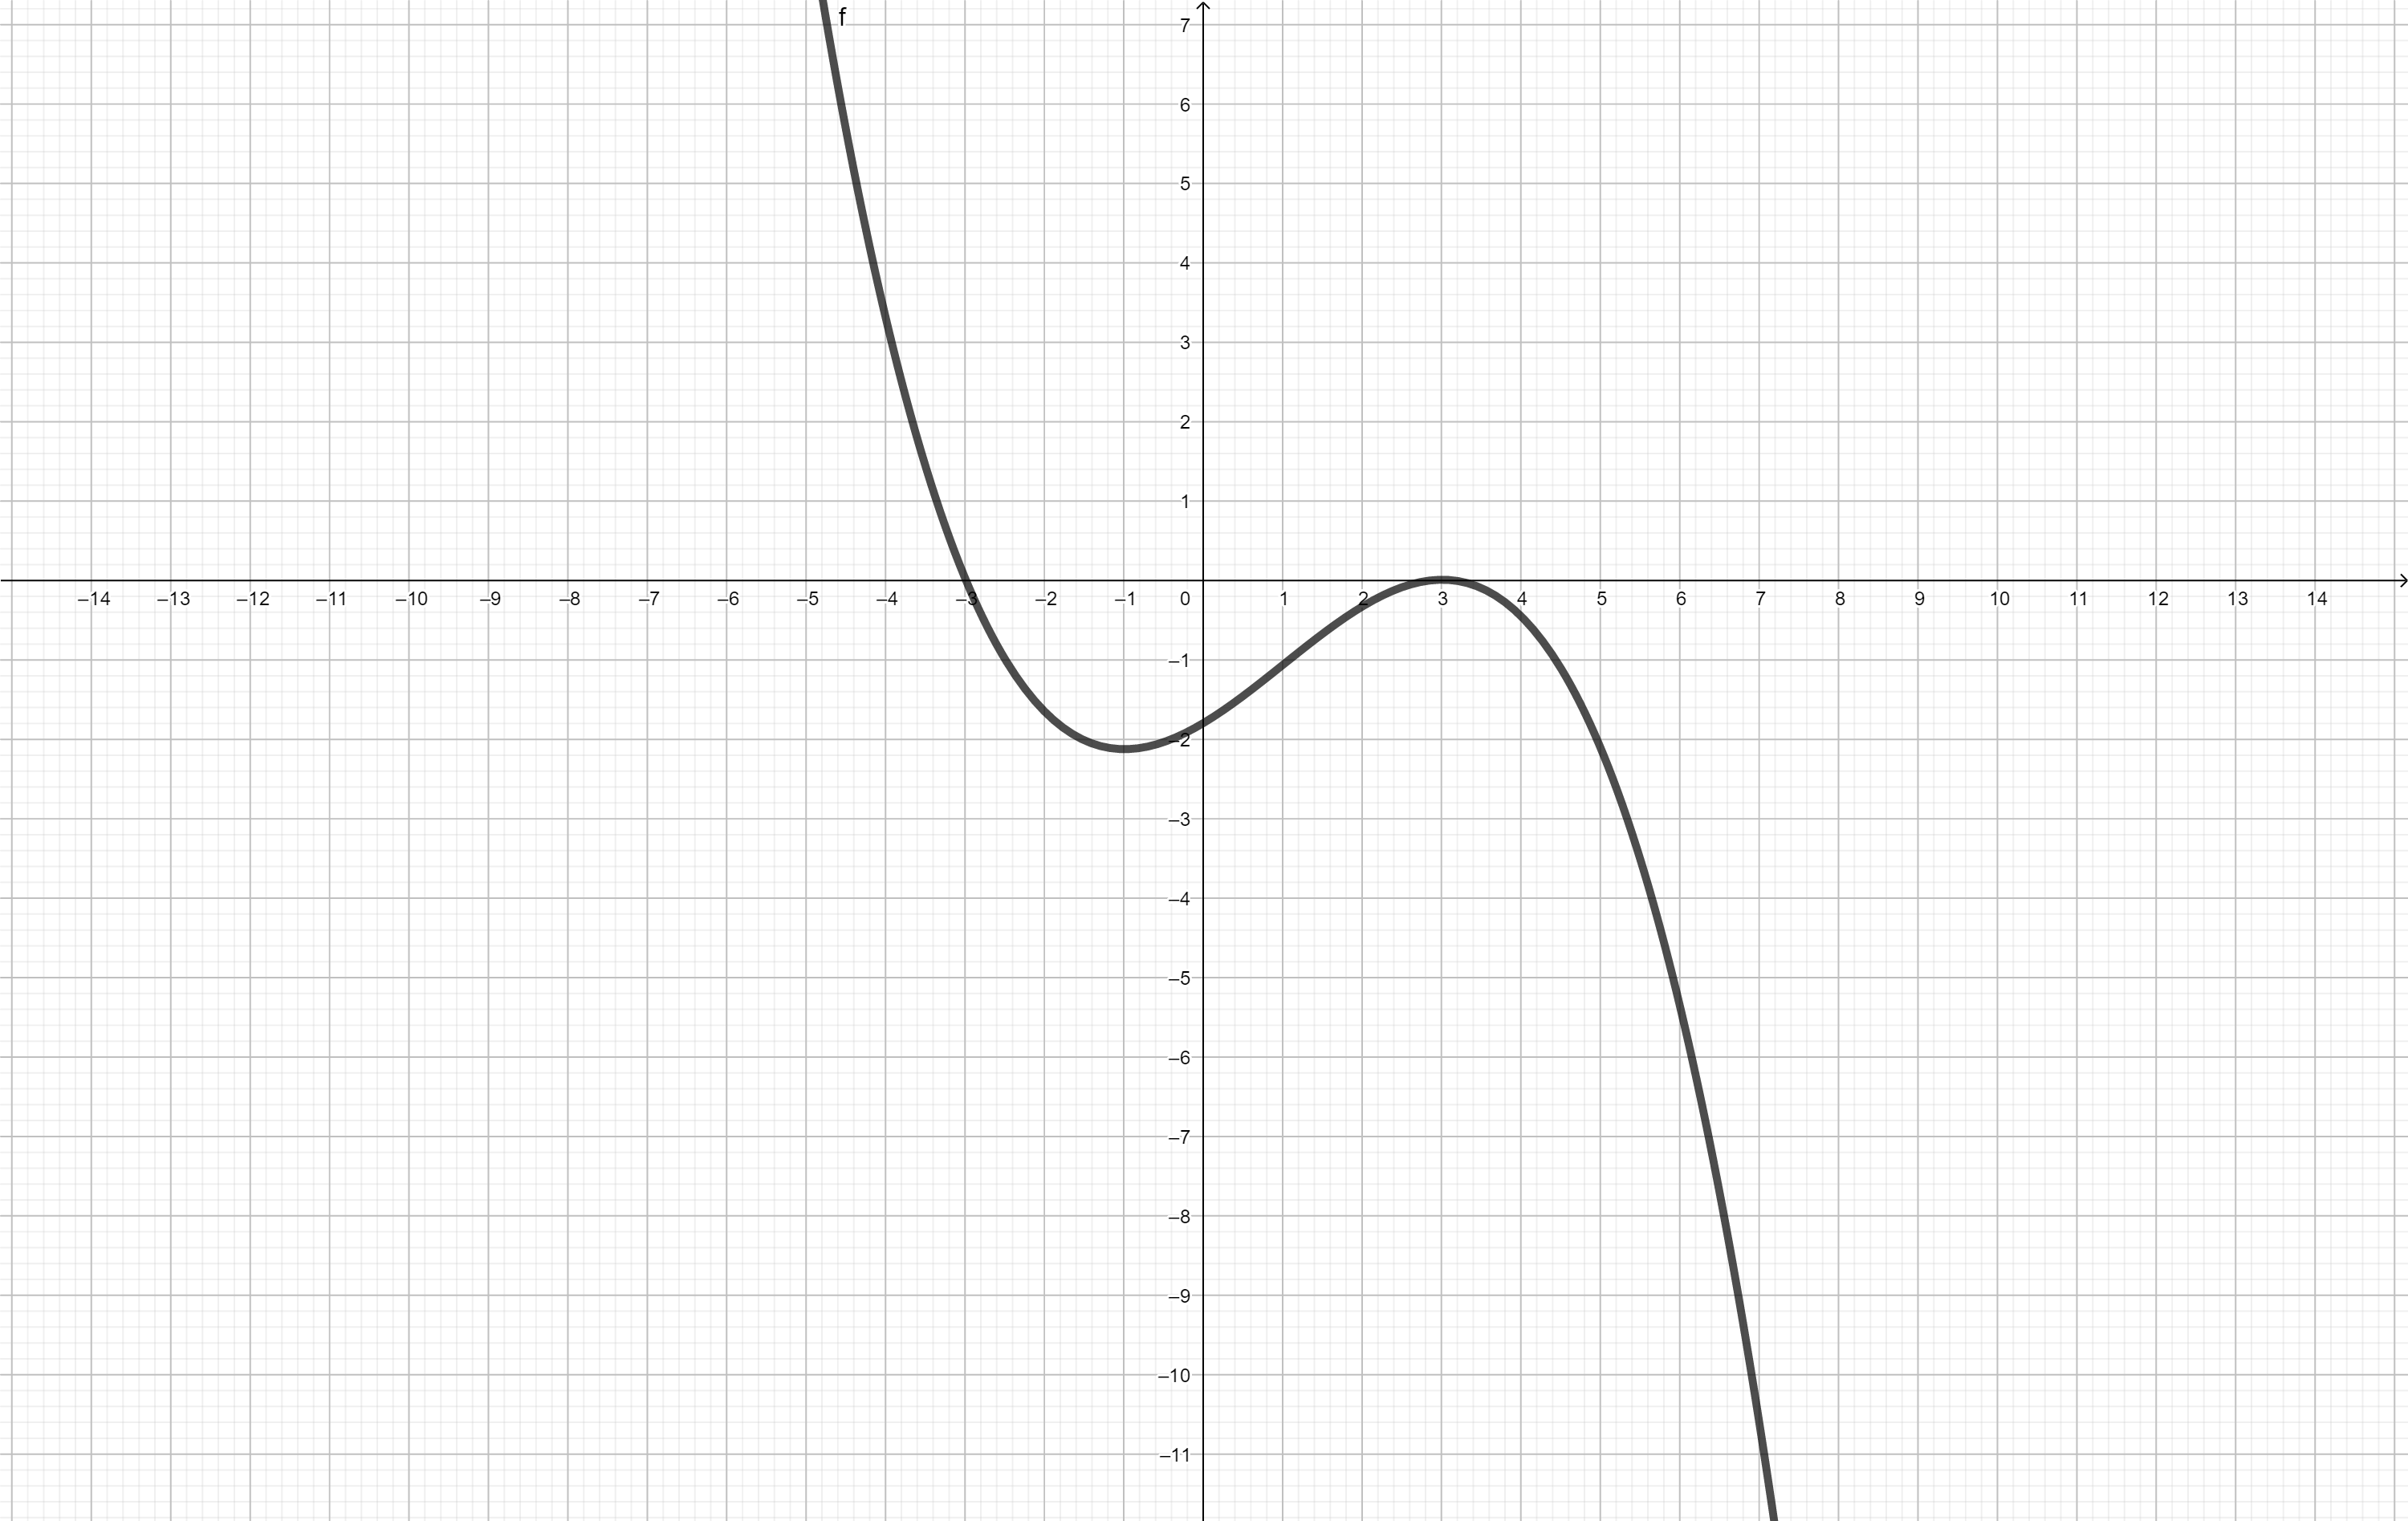
\includegraphics[width=4cm]{Bilder/G38}

\begin{addmargin}[-2cm]{0pt}
Nullstellen:

$x\rightarrow\infty:$

$x\rightarrow-\infty:$
\end{addmargin}

\newpage

\paragraph{Grad 4:}\textcolor{white}{.}

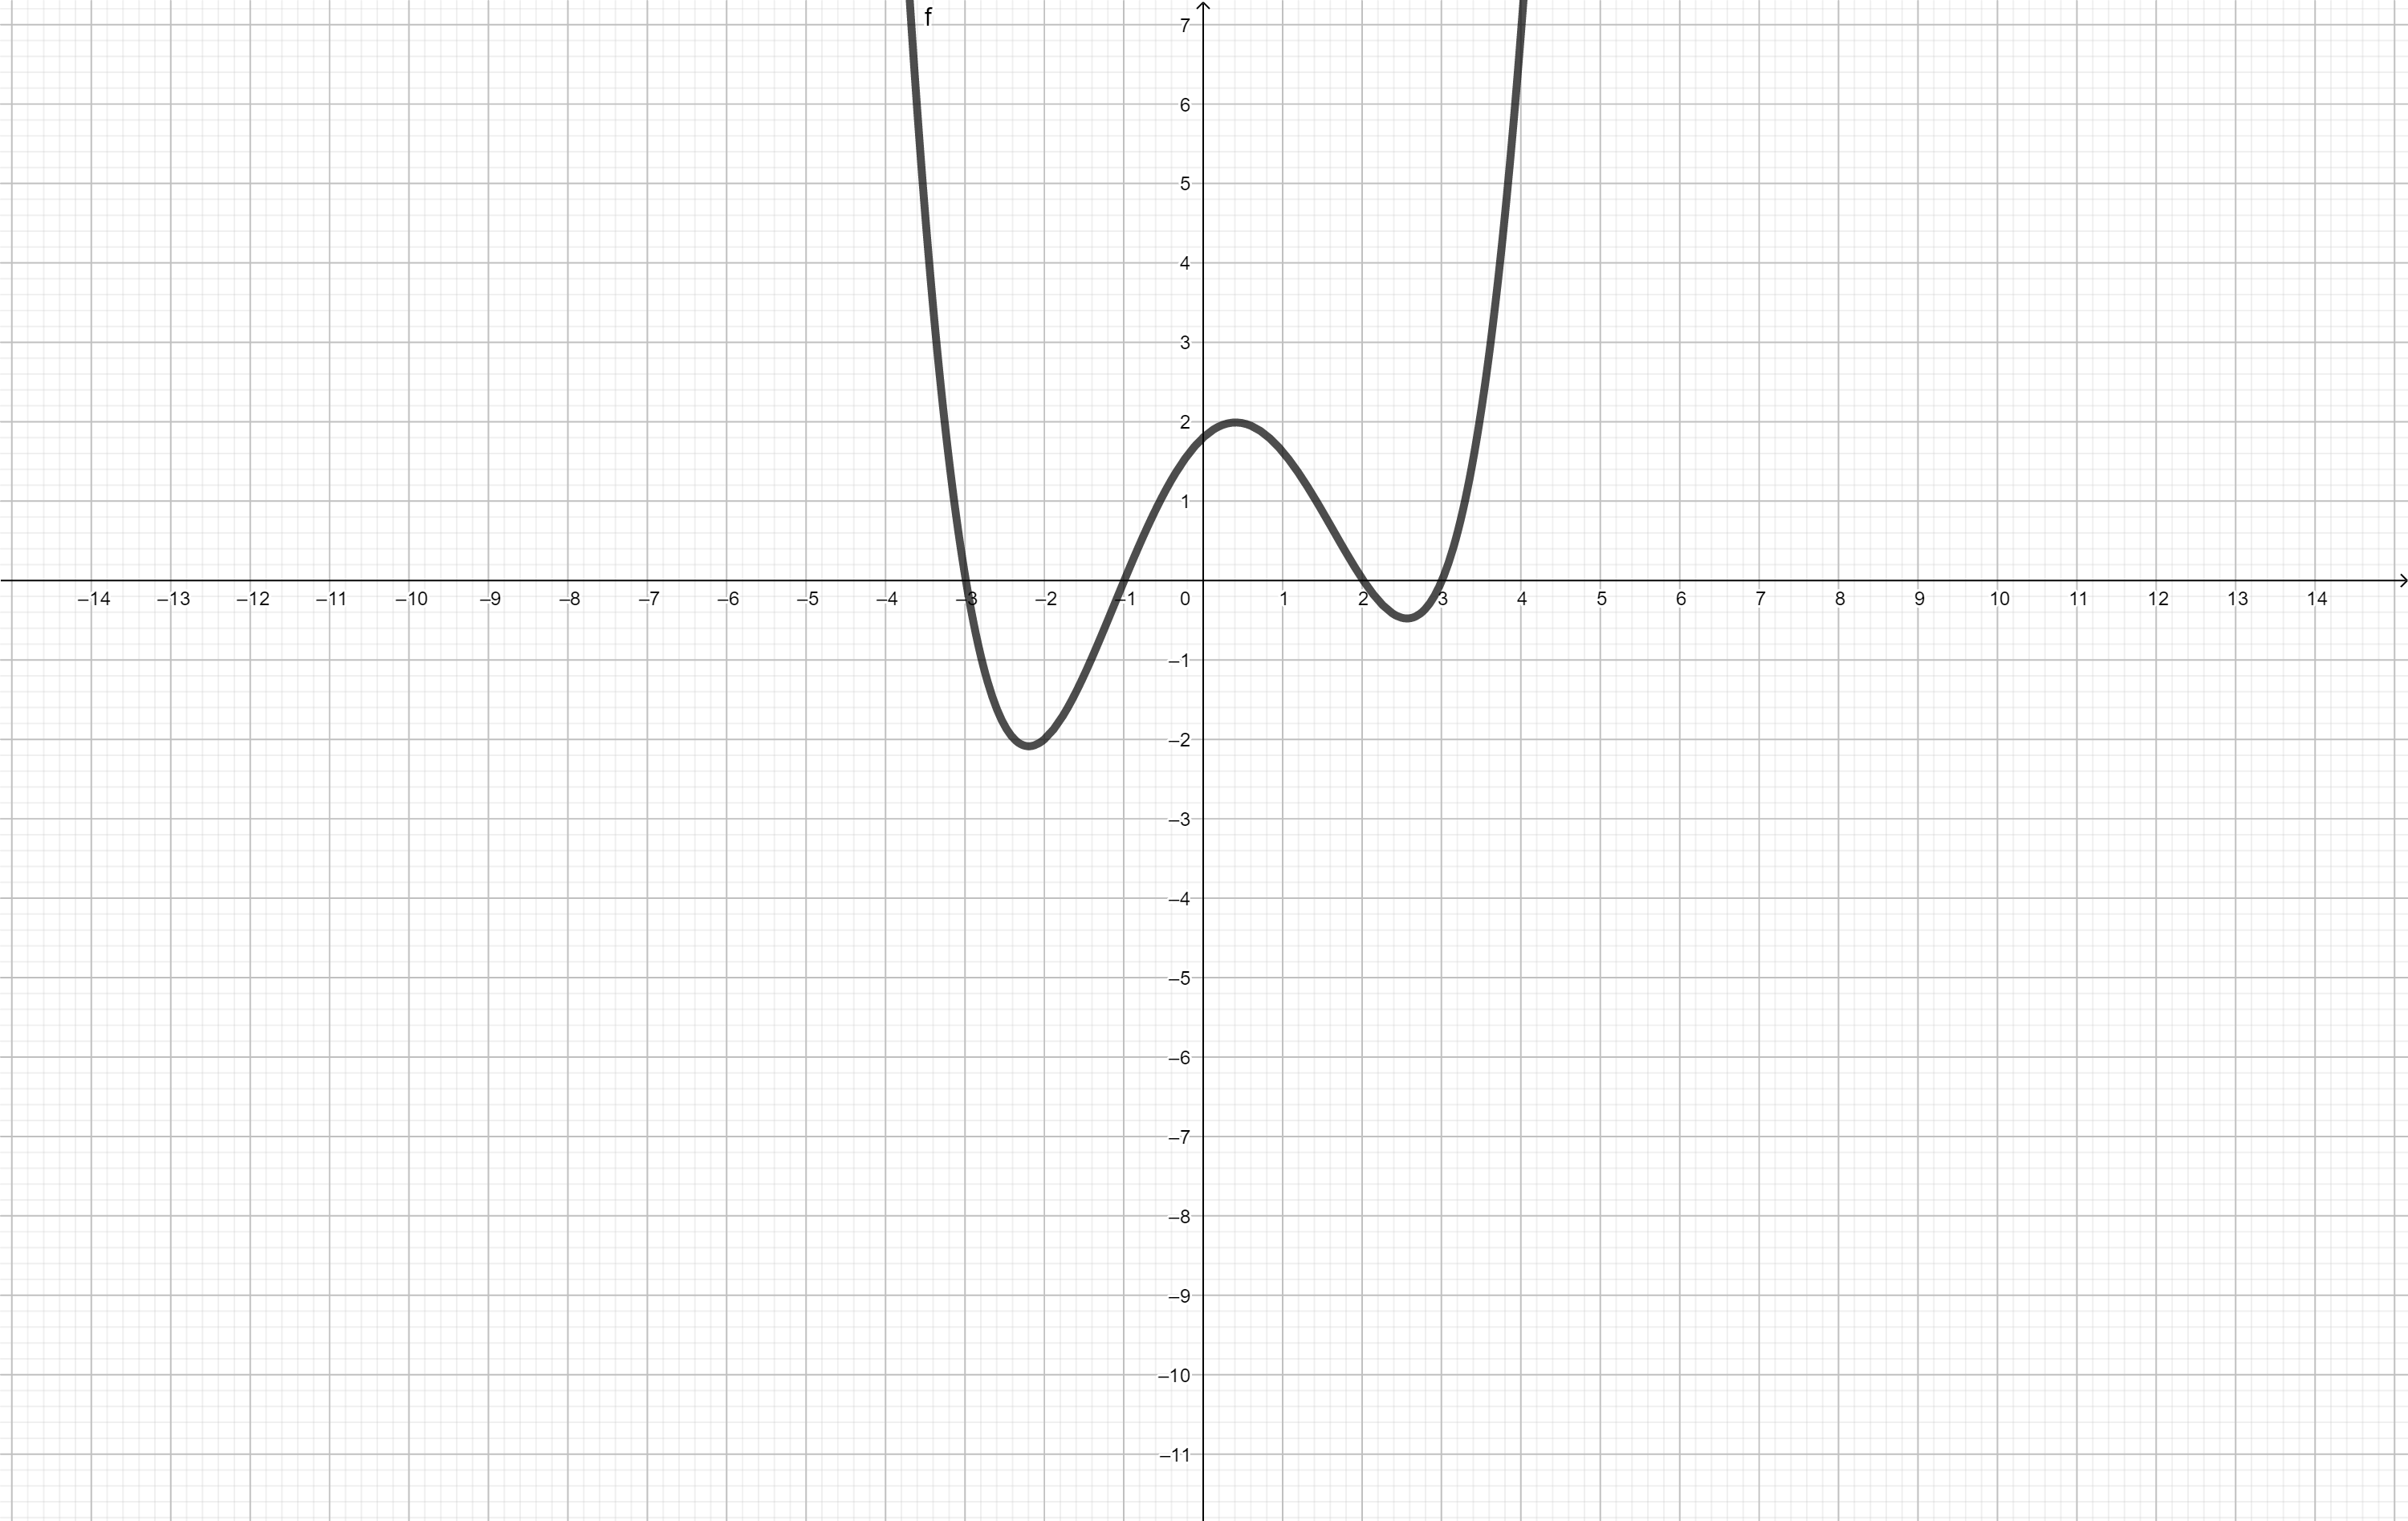
\includegraphics[width=4cm]{Bilder/G41}\hfill
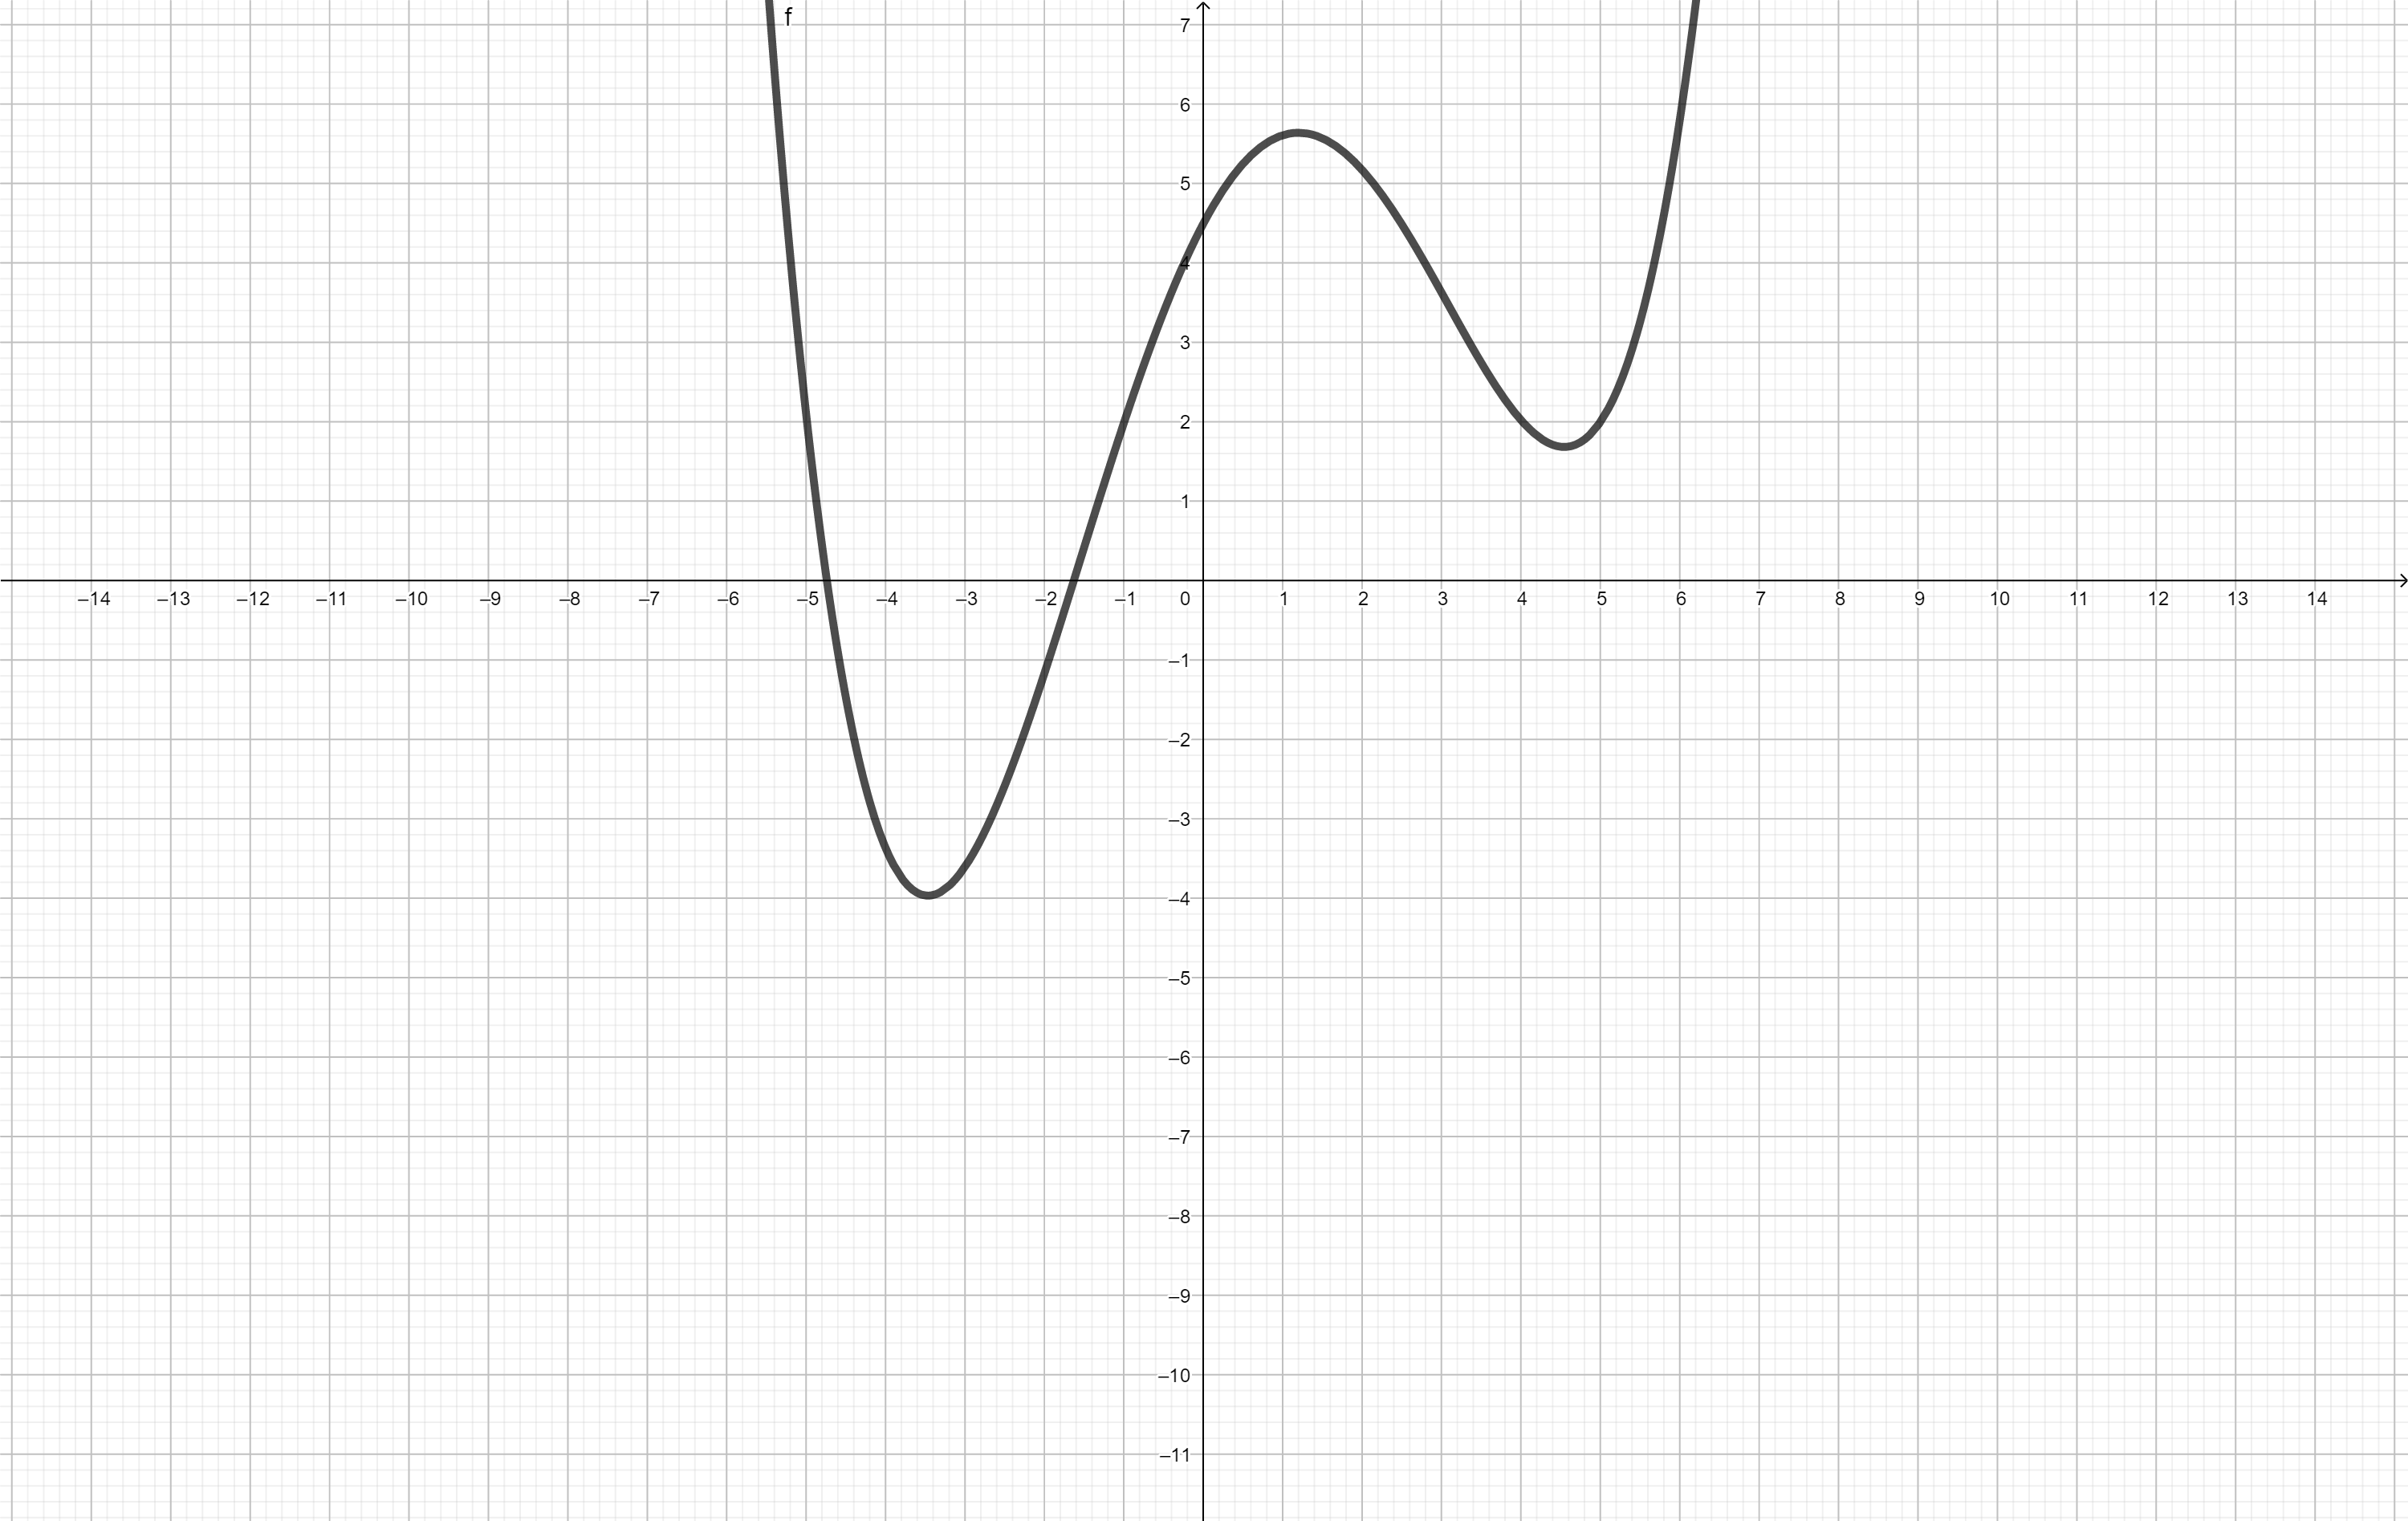
\includegraphics[width=4cm]{Bilder/G42}\hfill
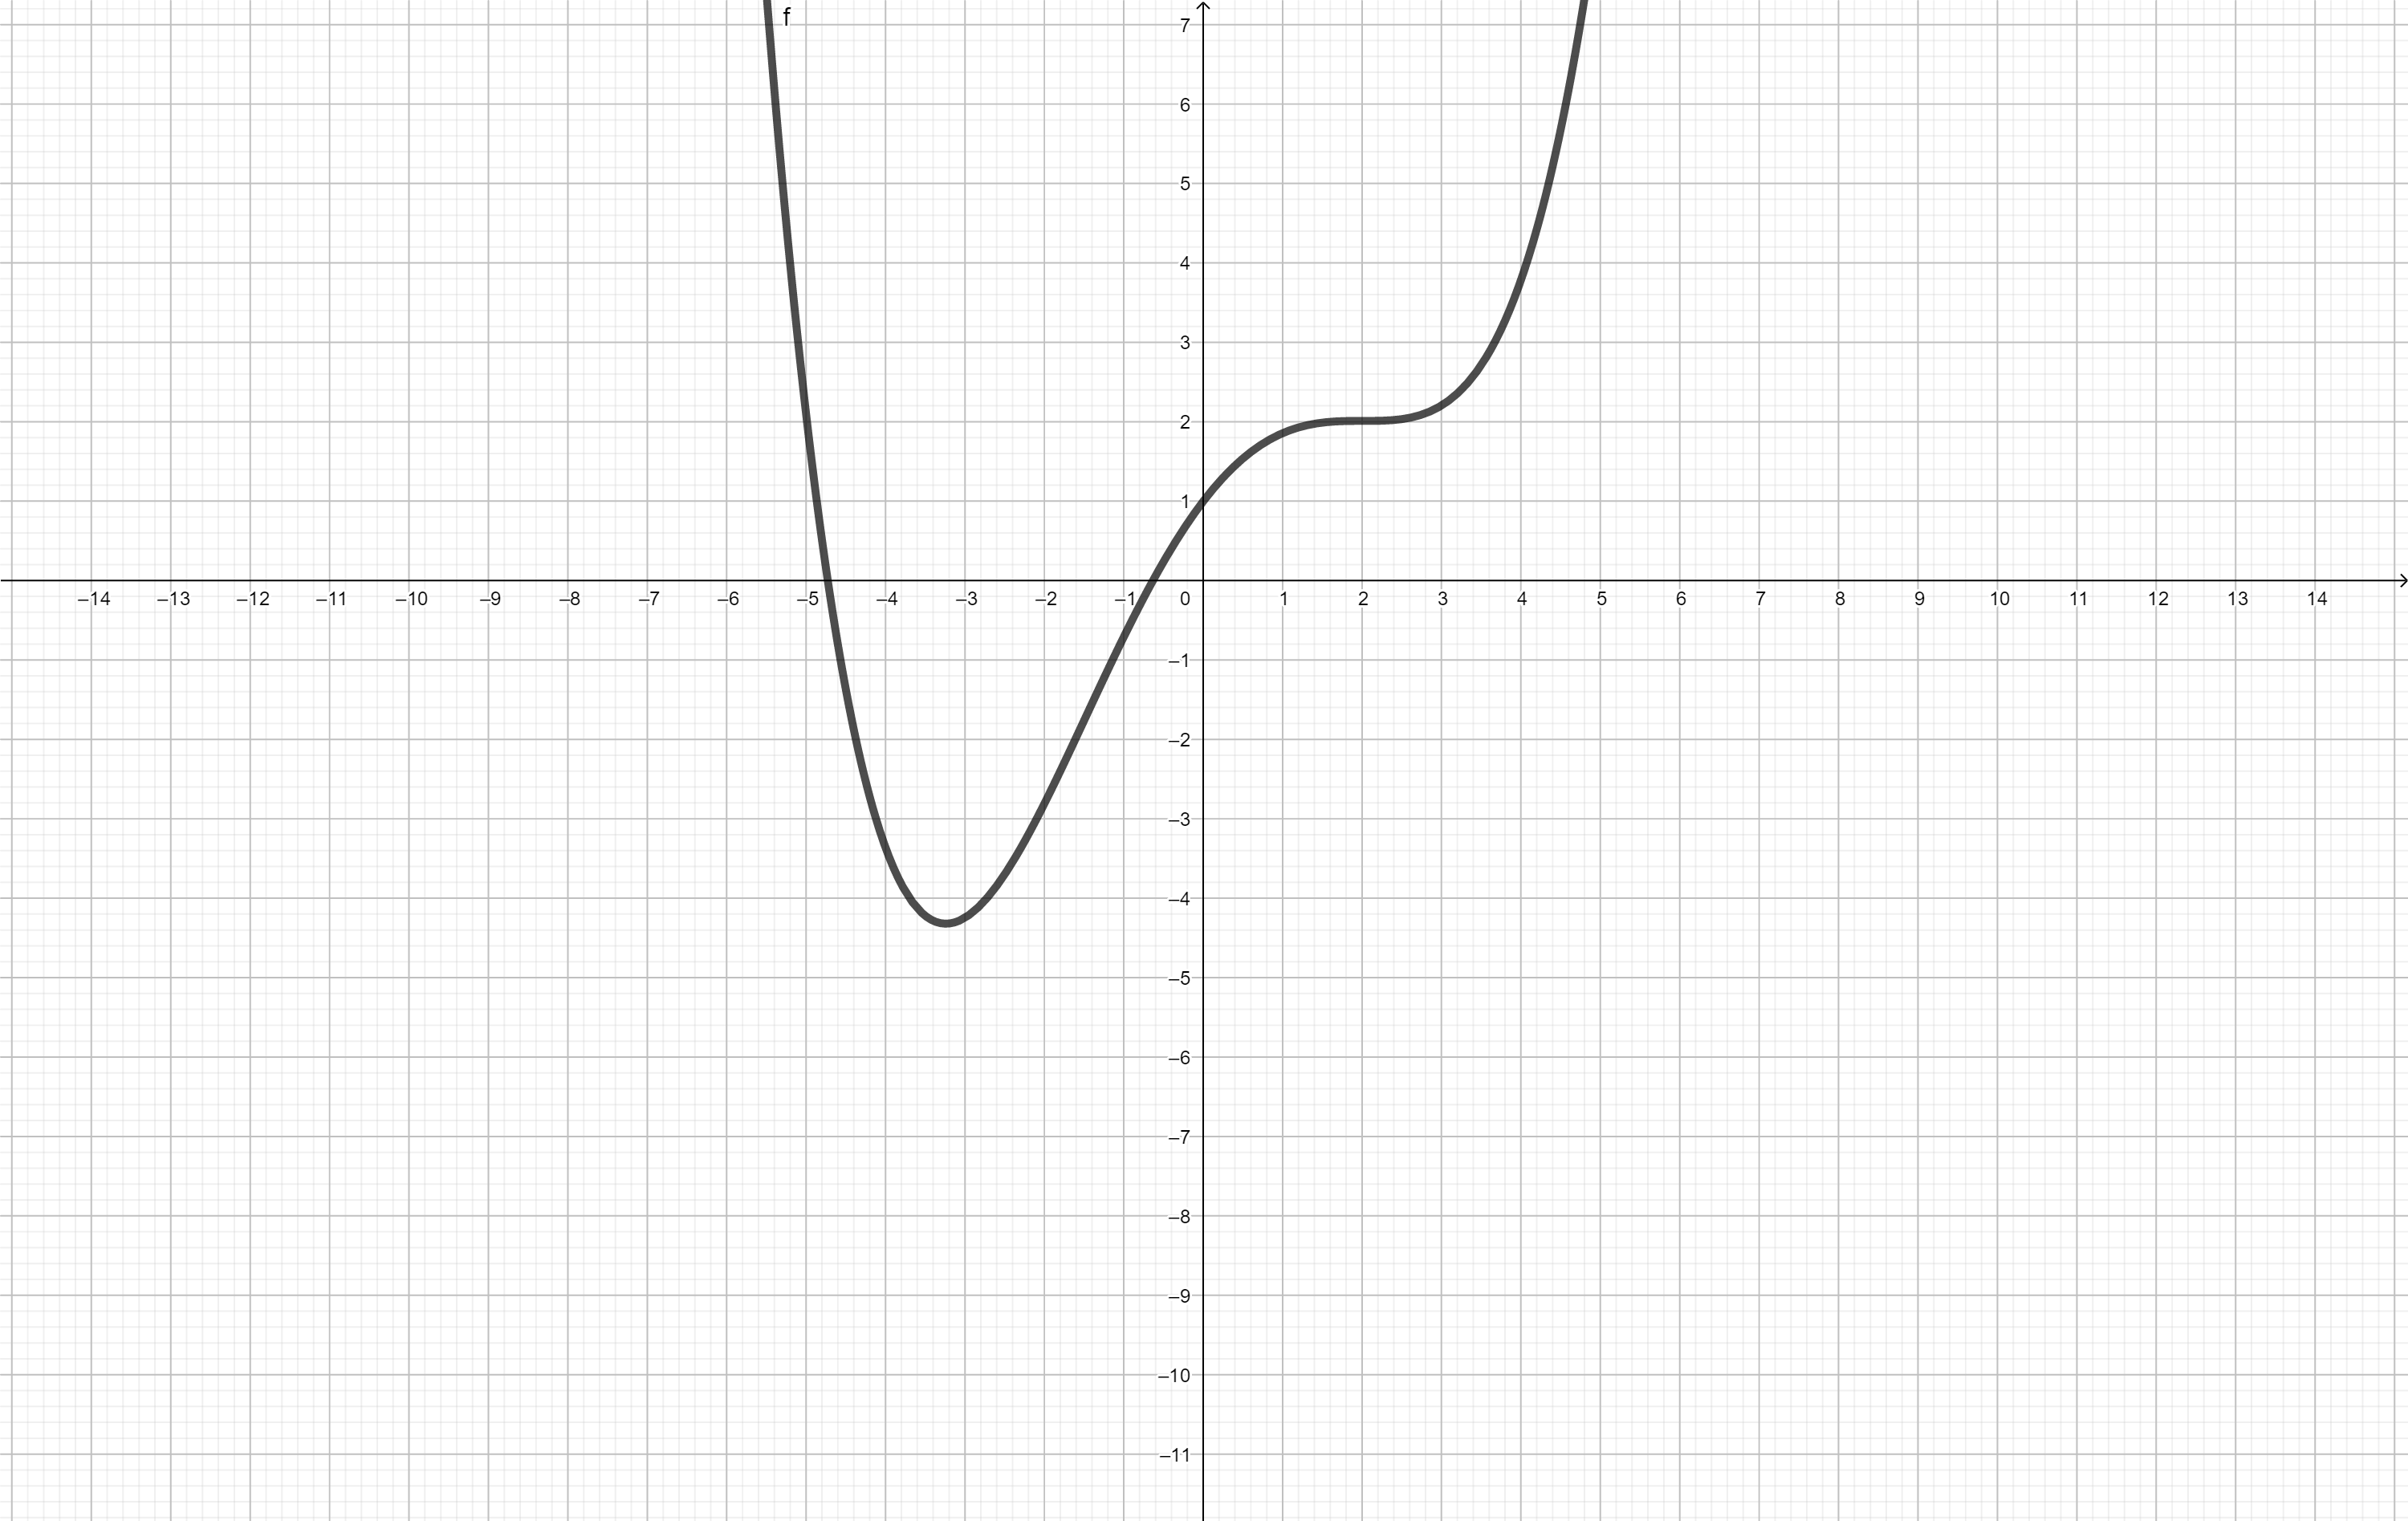
\includegraphics[width=4cm]{Bilder/G43}\hfill
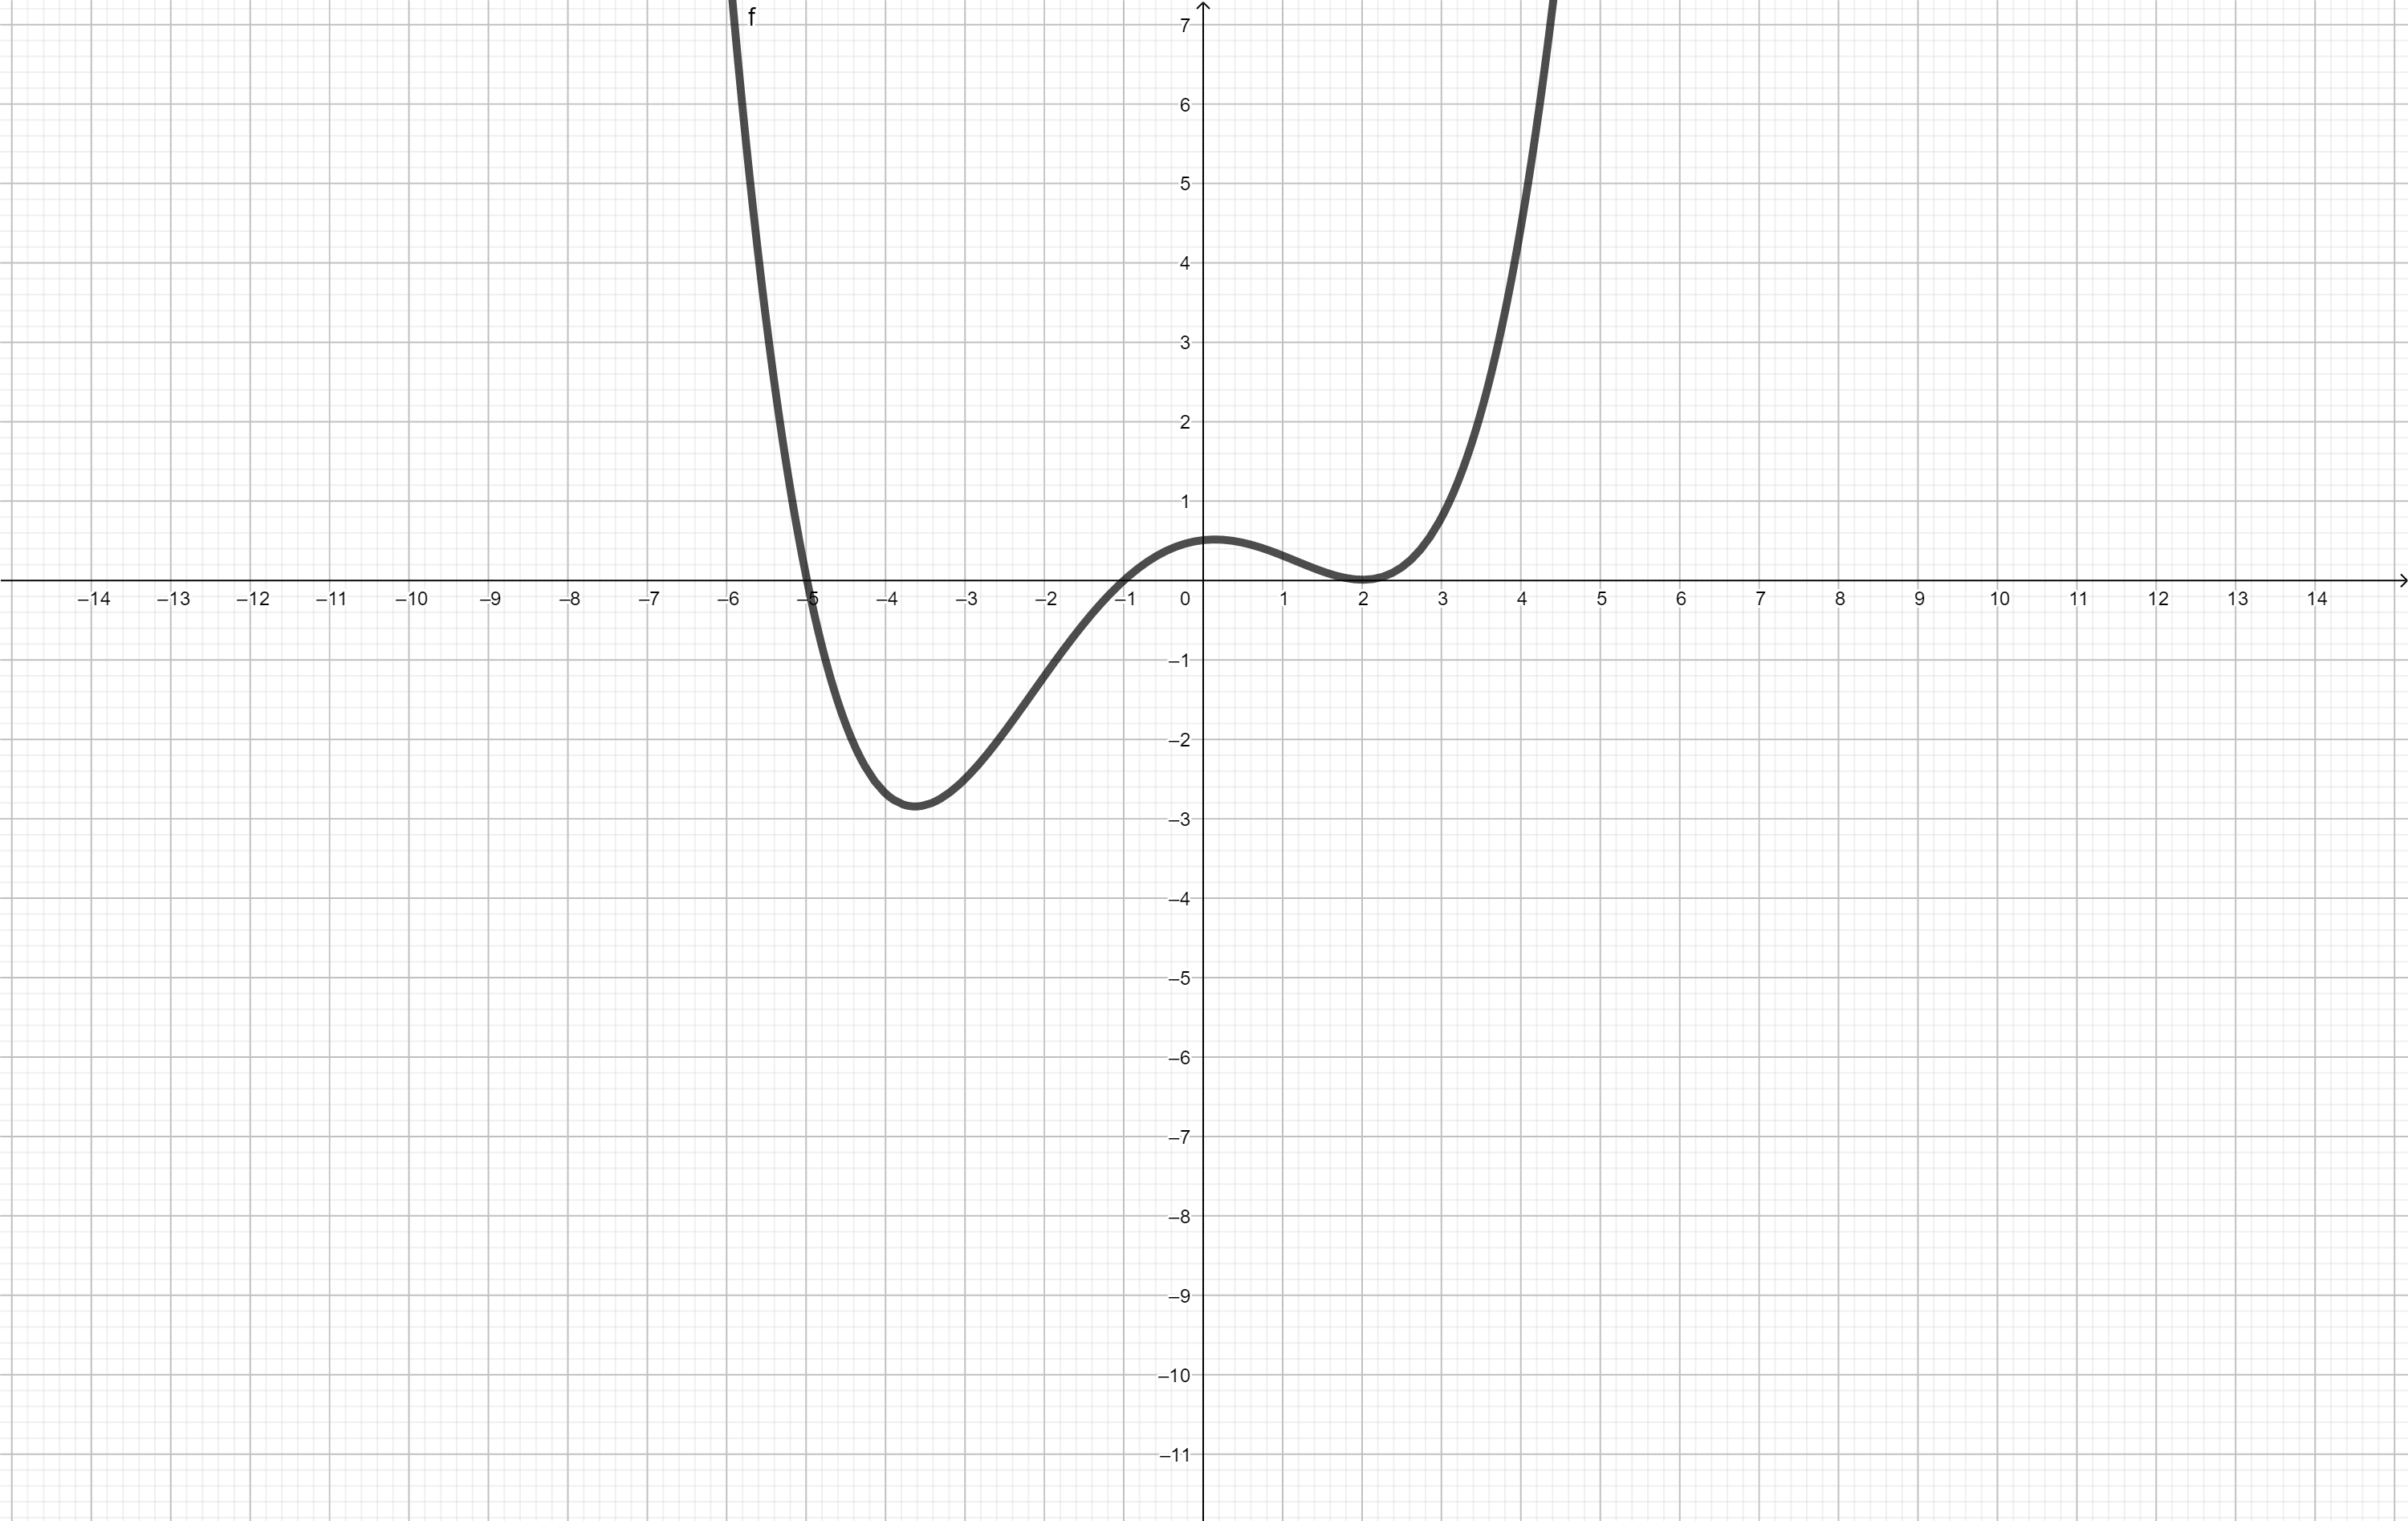
\includegraphics[width=4cm]{Bilder/G44}

\begin{addmargin}[-2cm]{0pt}
Nullstellen:

$x\rightarrow\infty:$

$x\rightarrow-\infty:$
\end{addmargin}

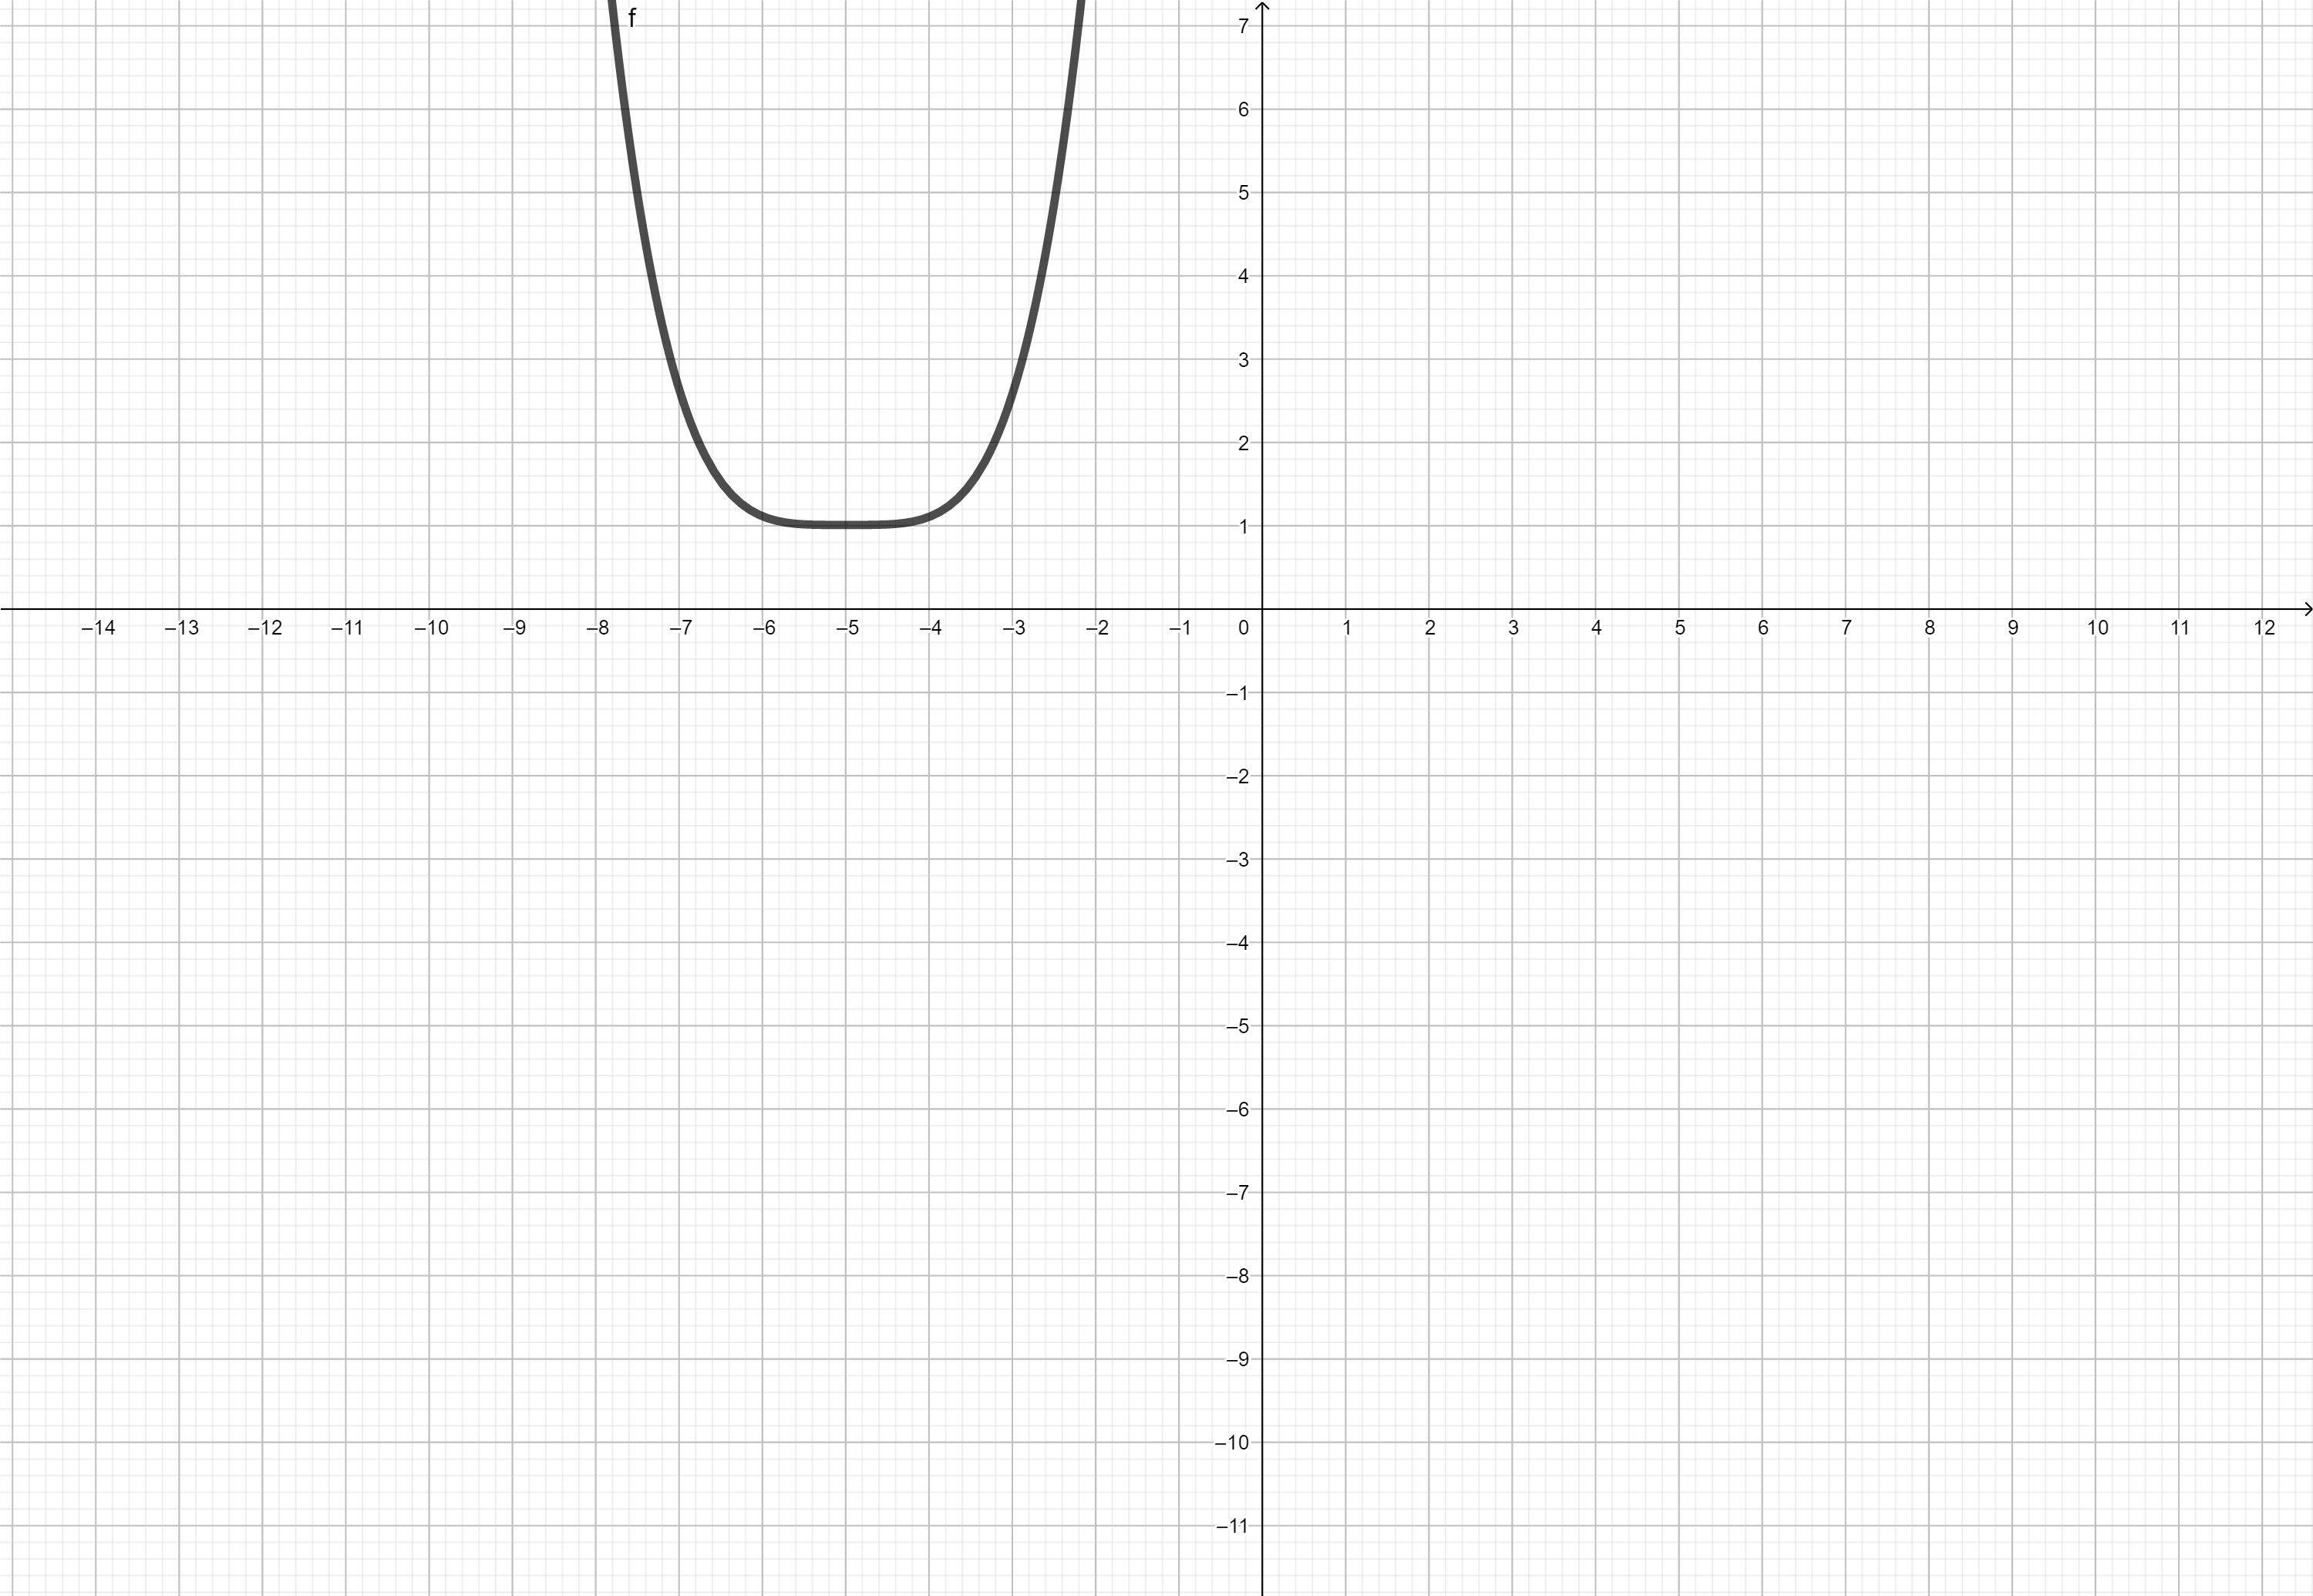
\includegraphics[width=4cm]{Bilder/G45}\hfill
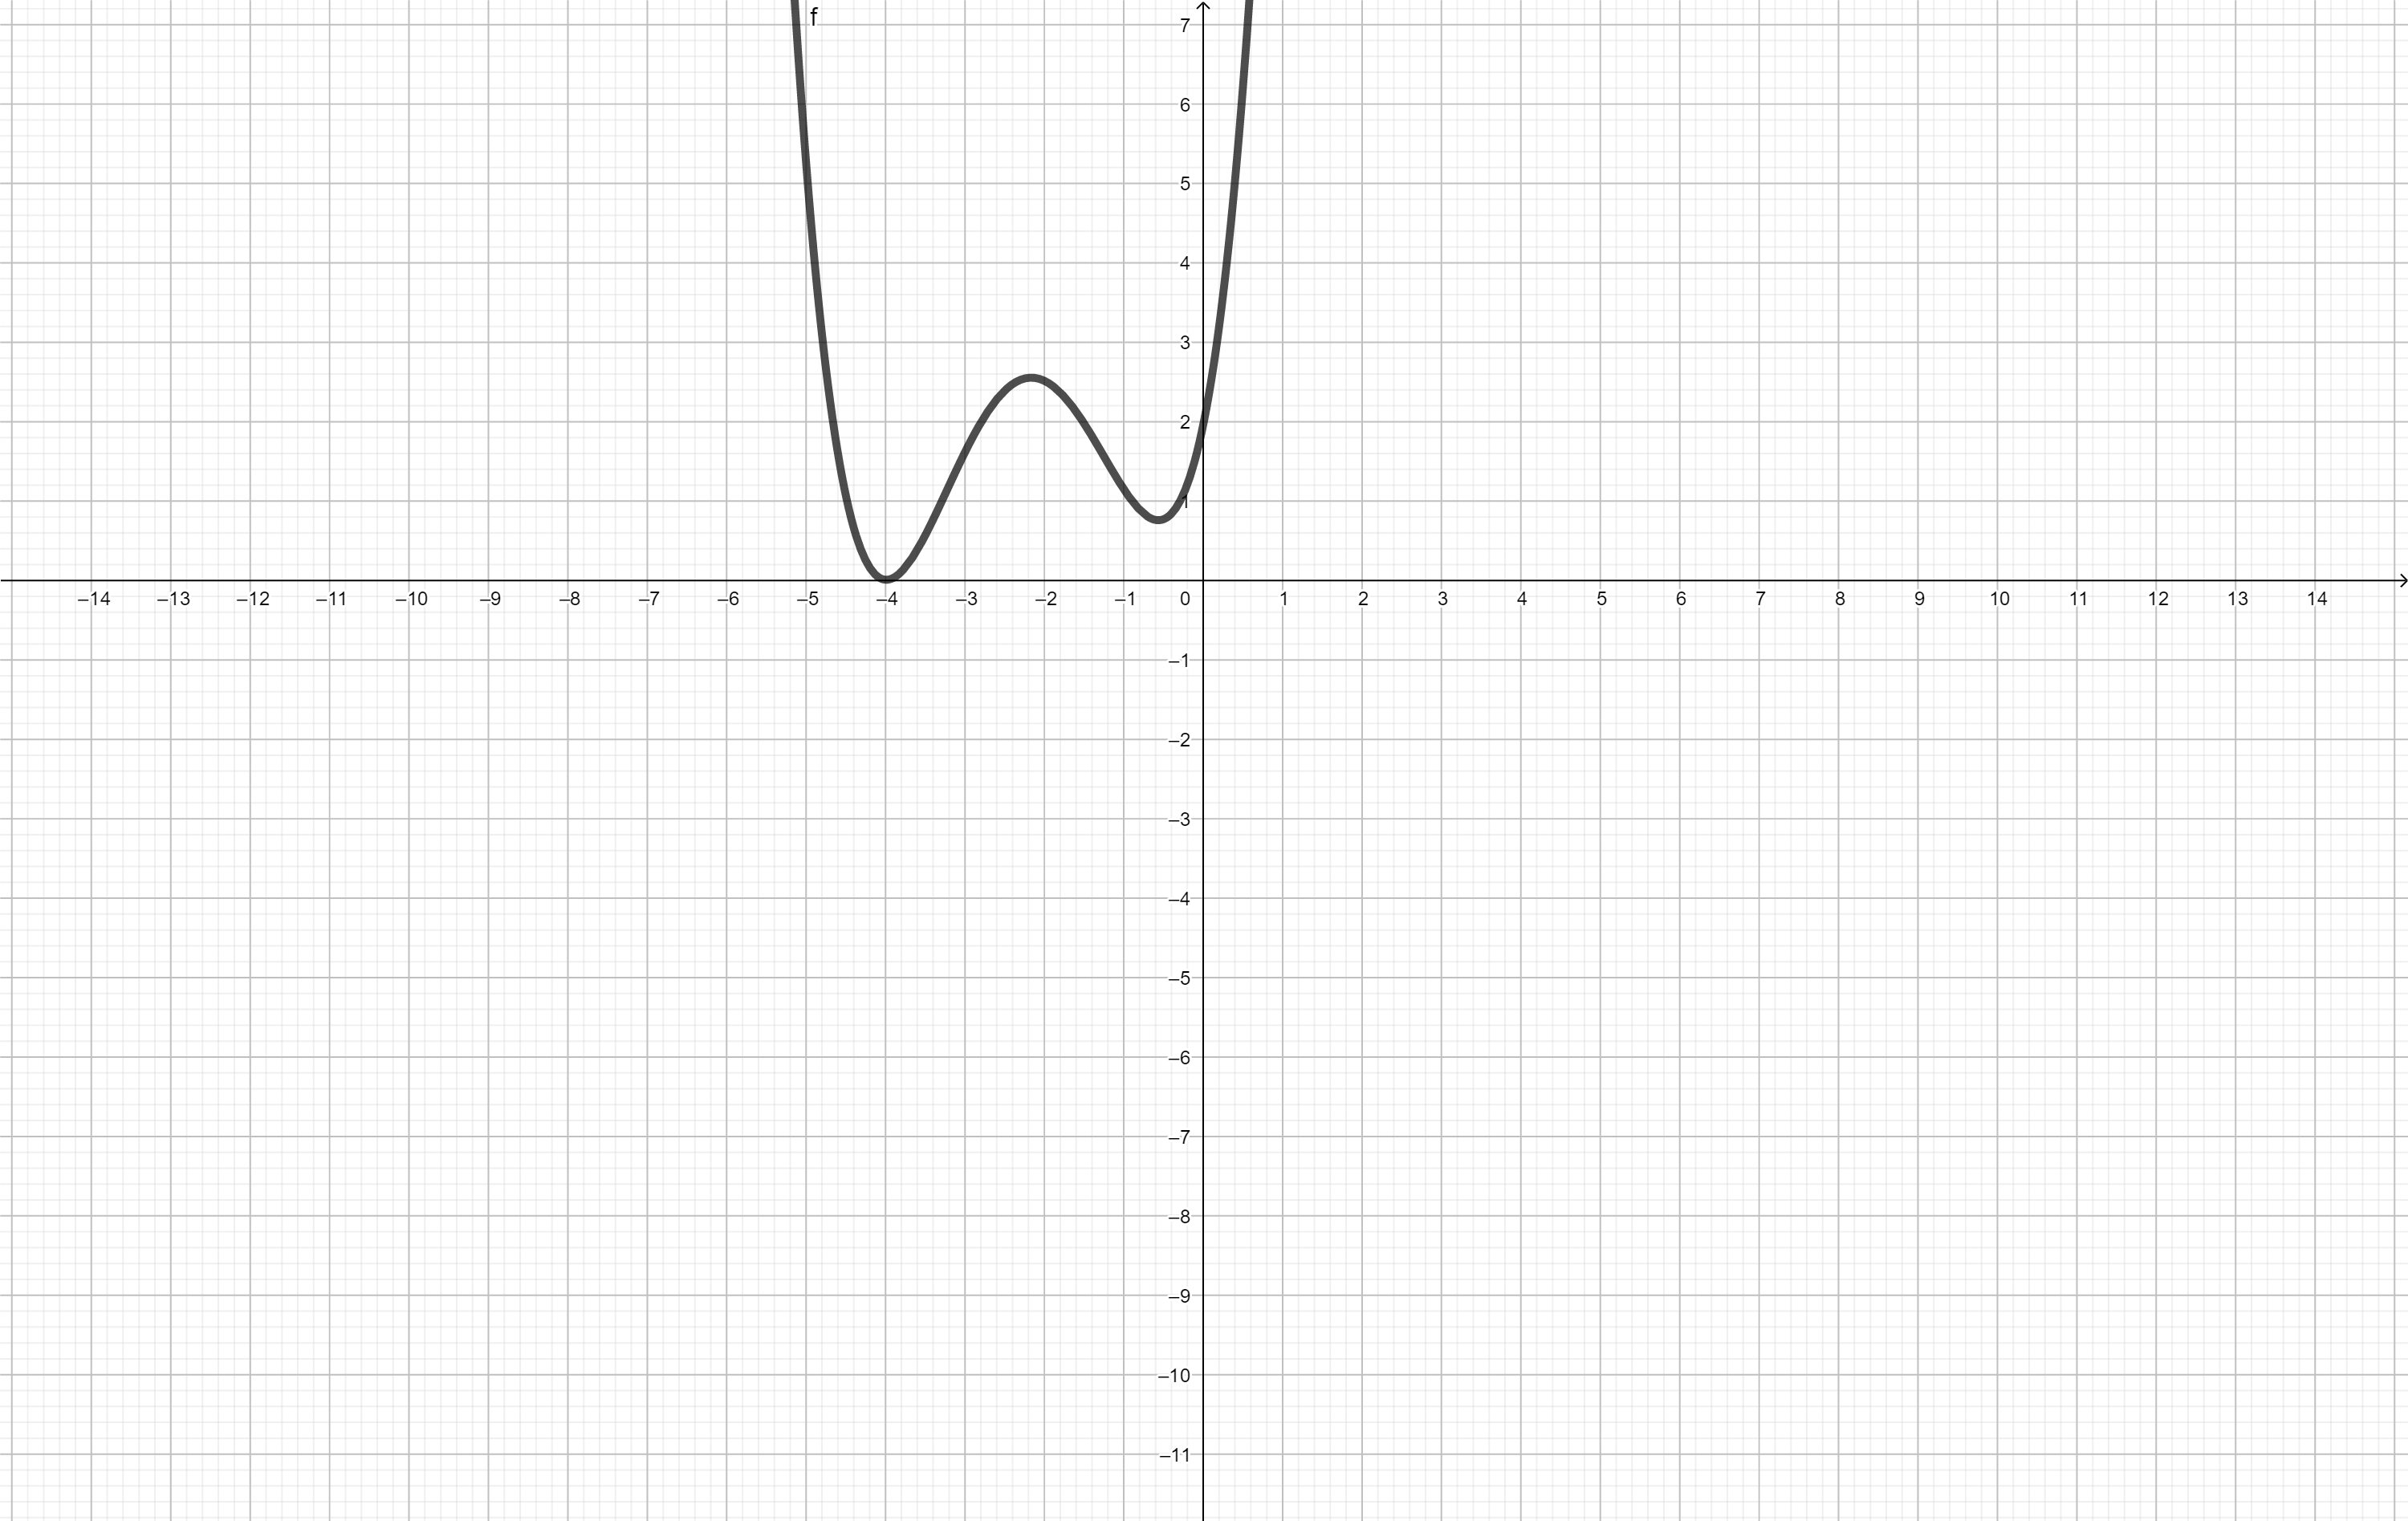
\includegraphics[width=4cm]{Bilder/G46}\hfill
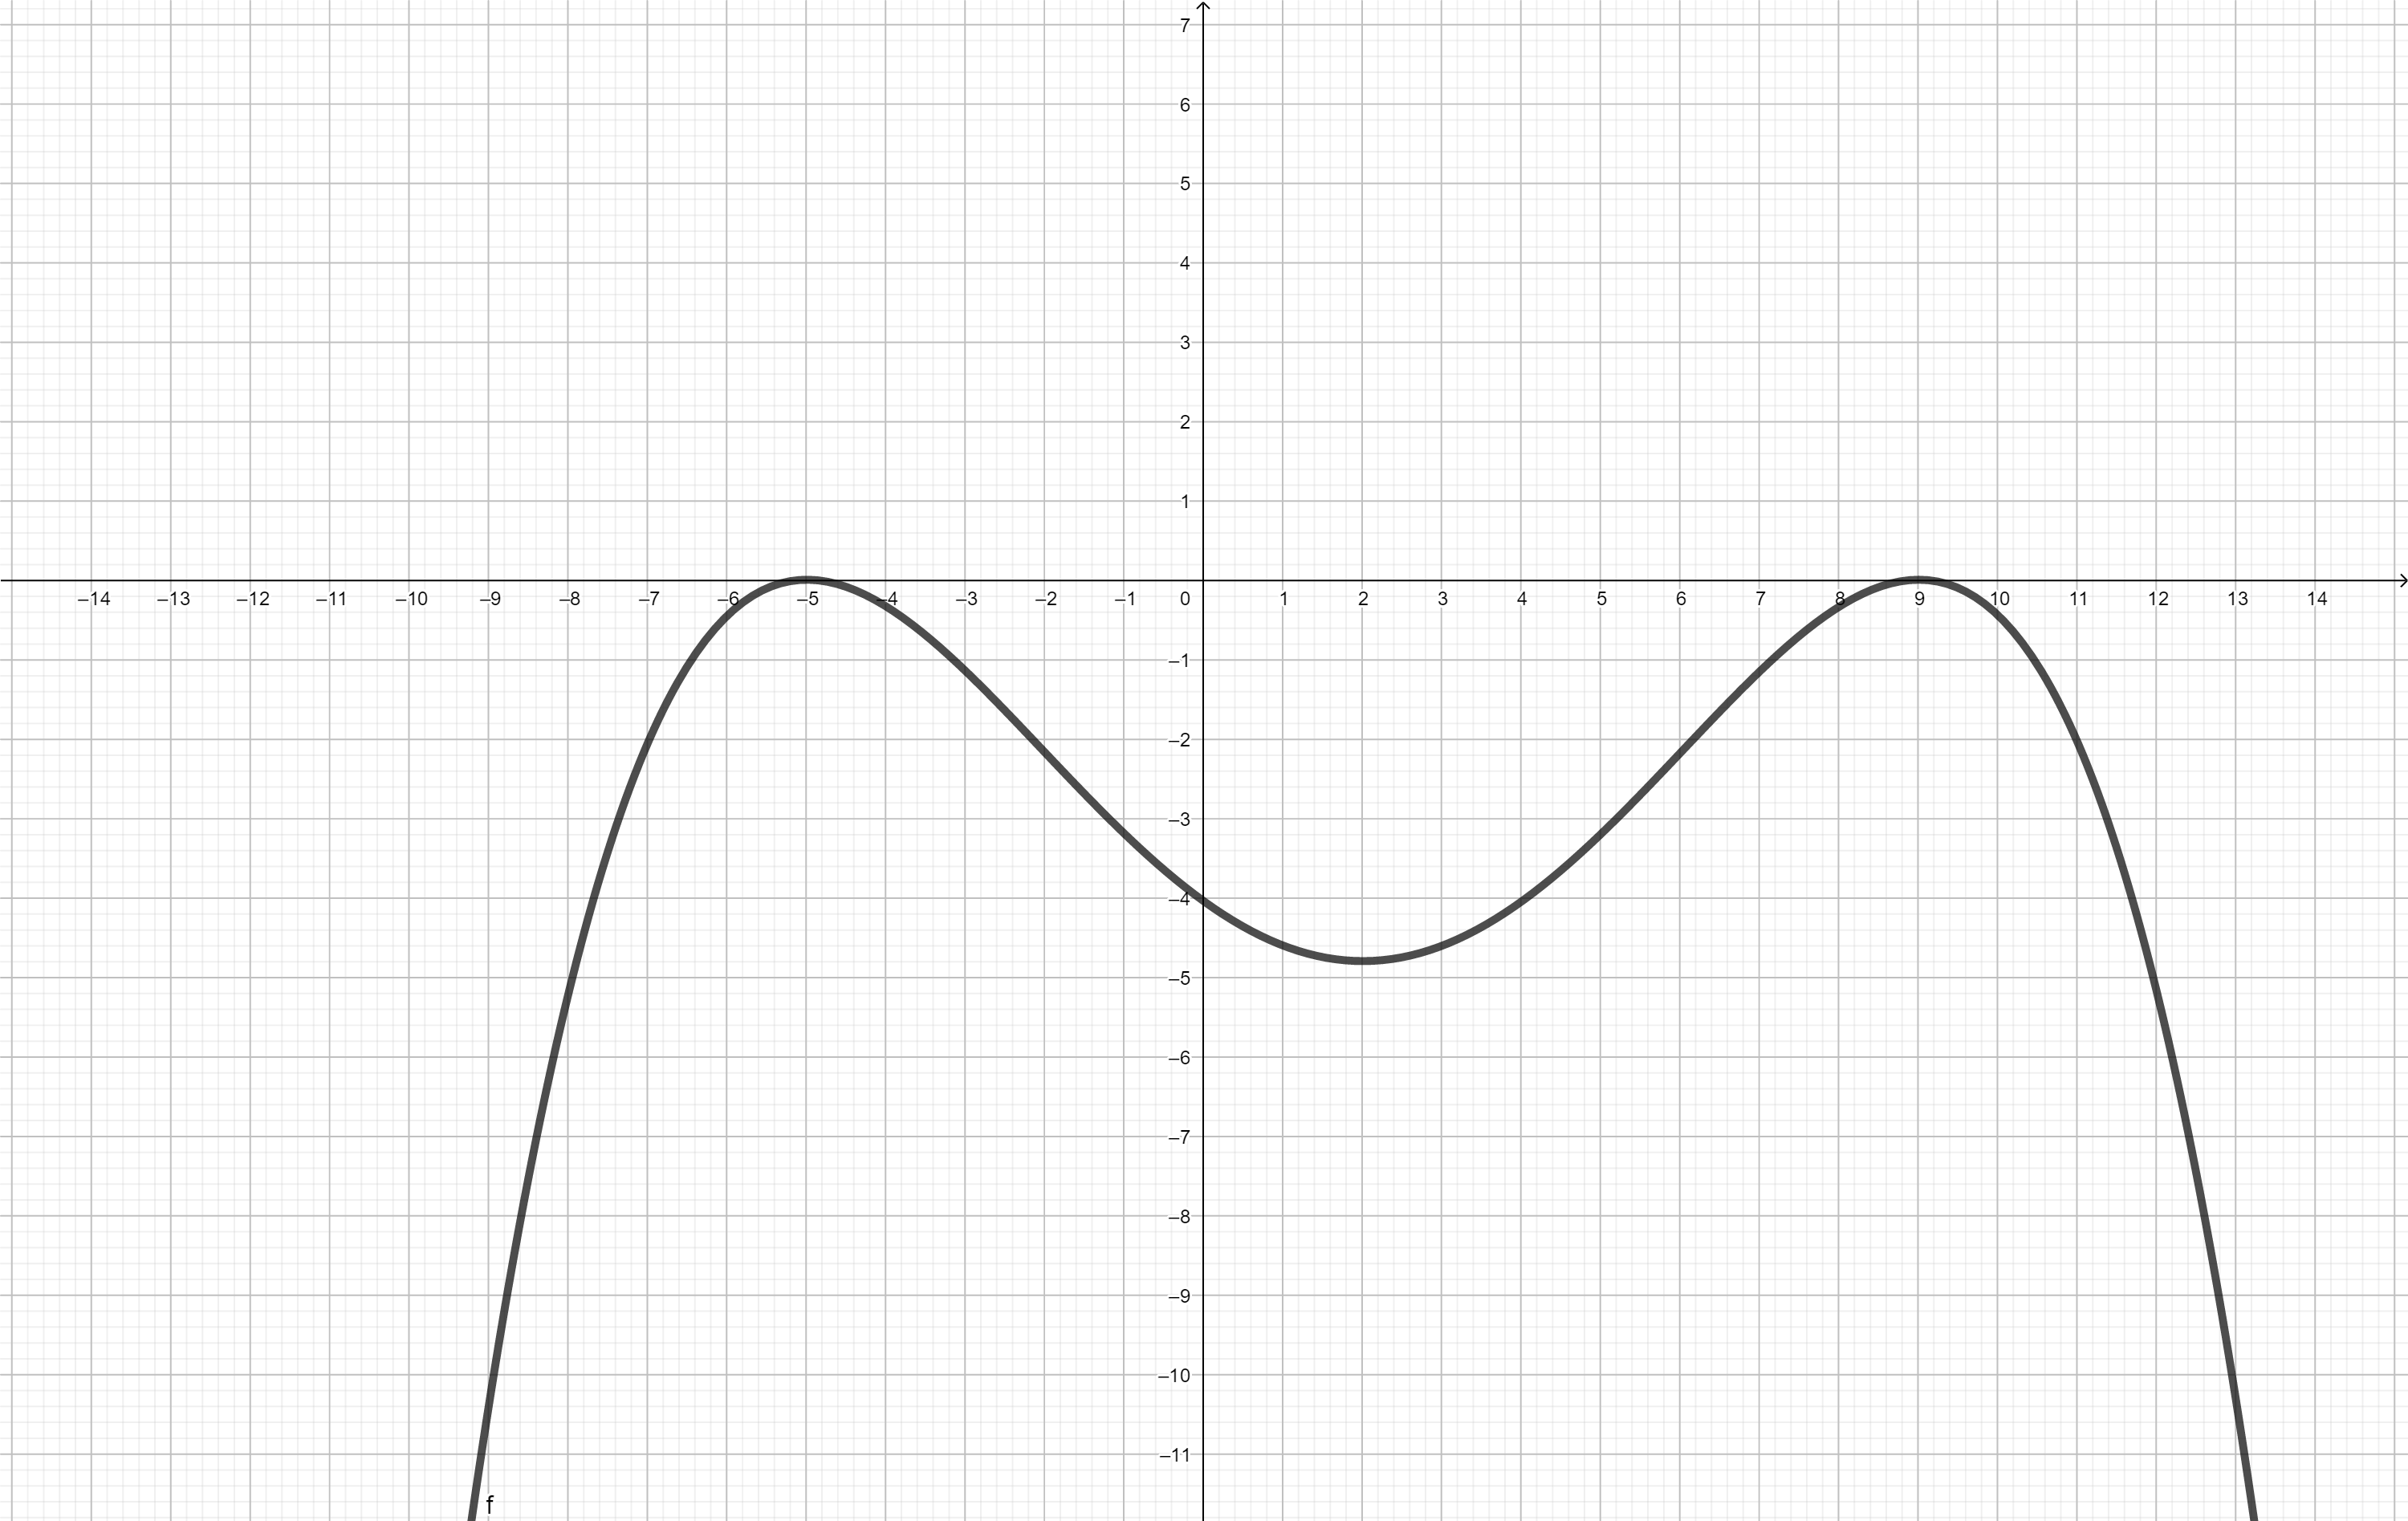
\includegraphics[width=4cm]{Bilder/G47}\hfill
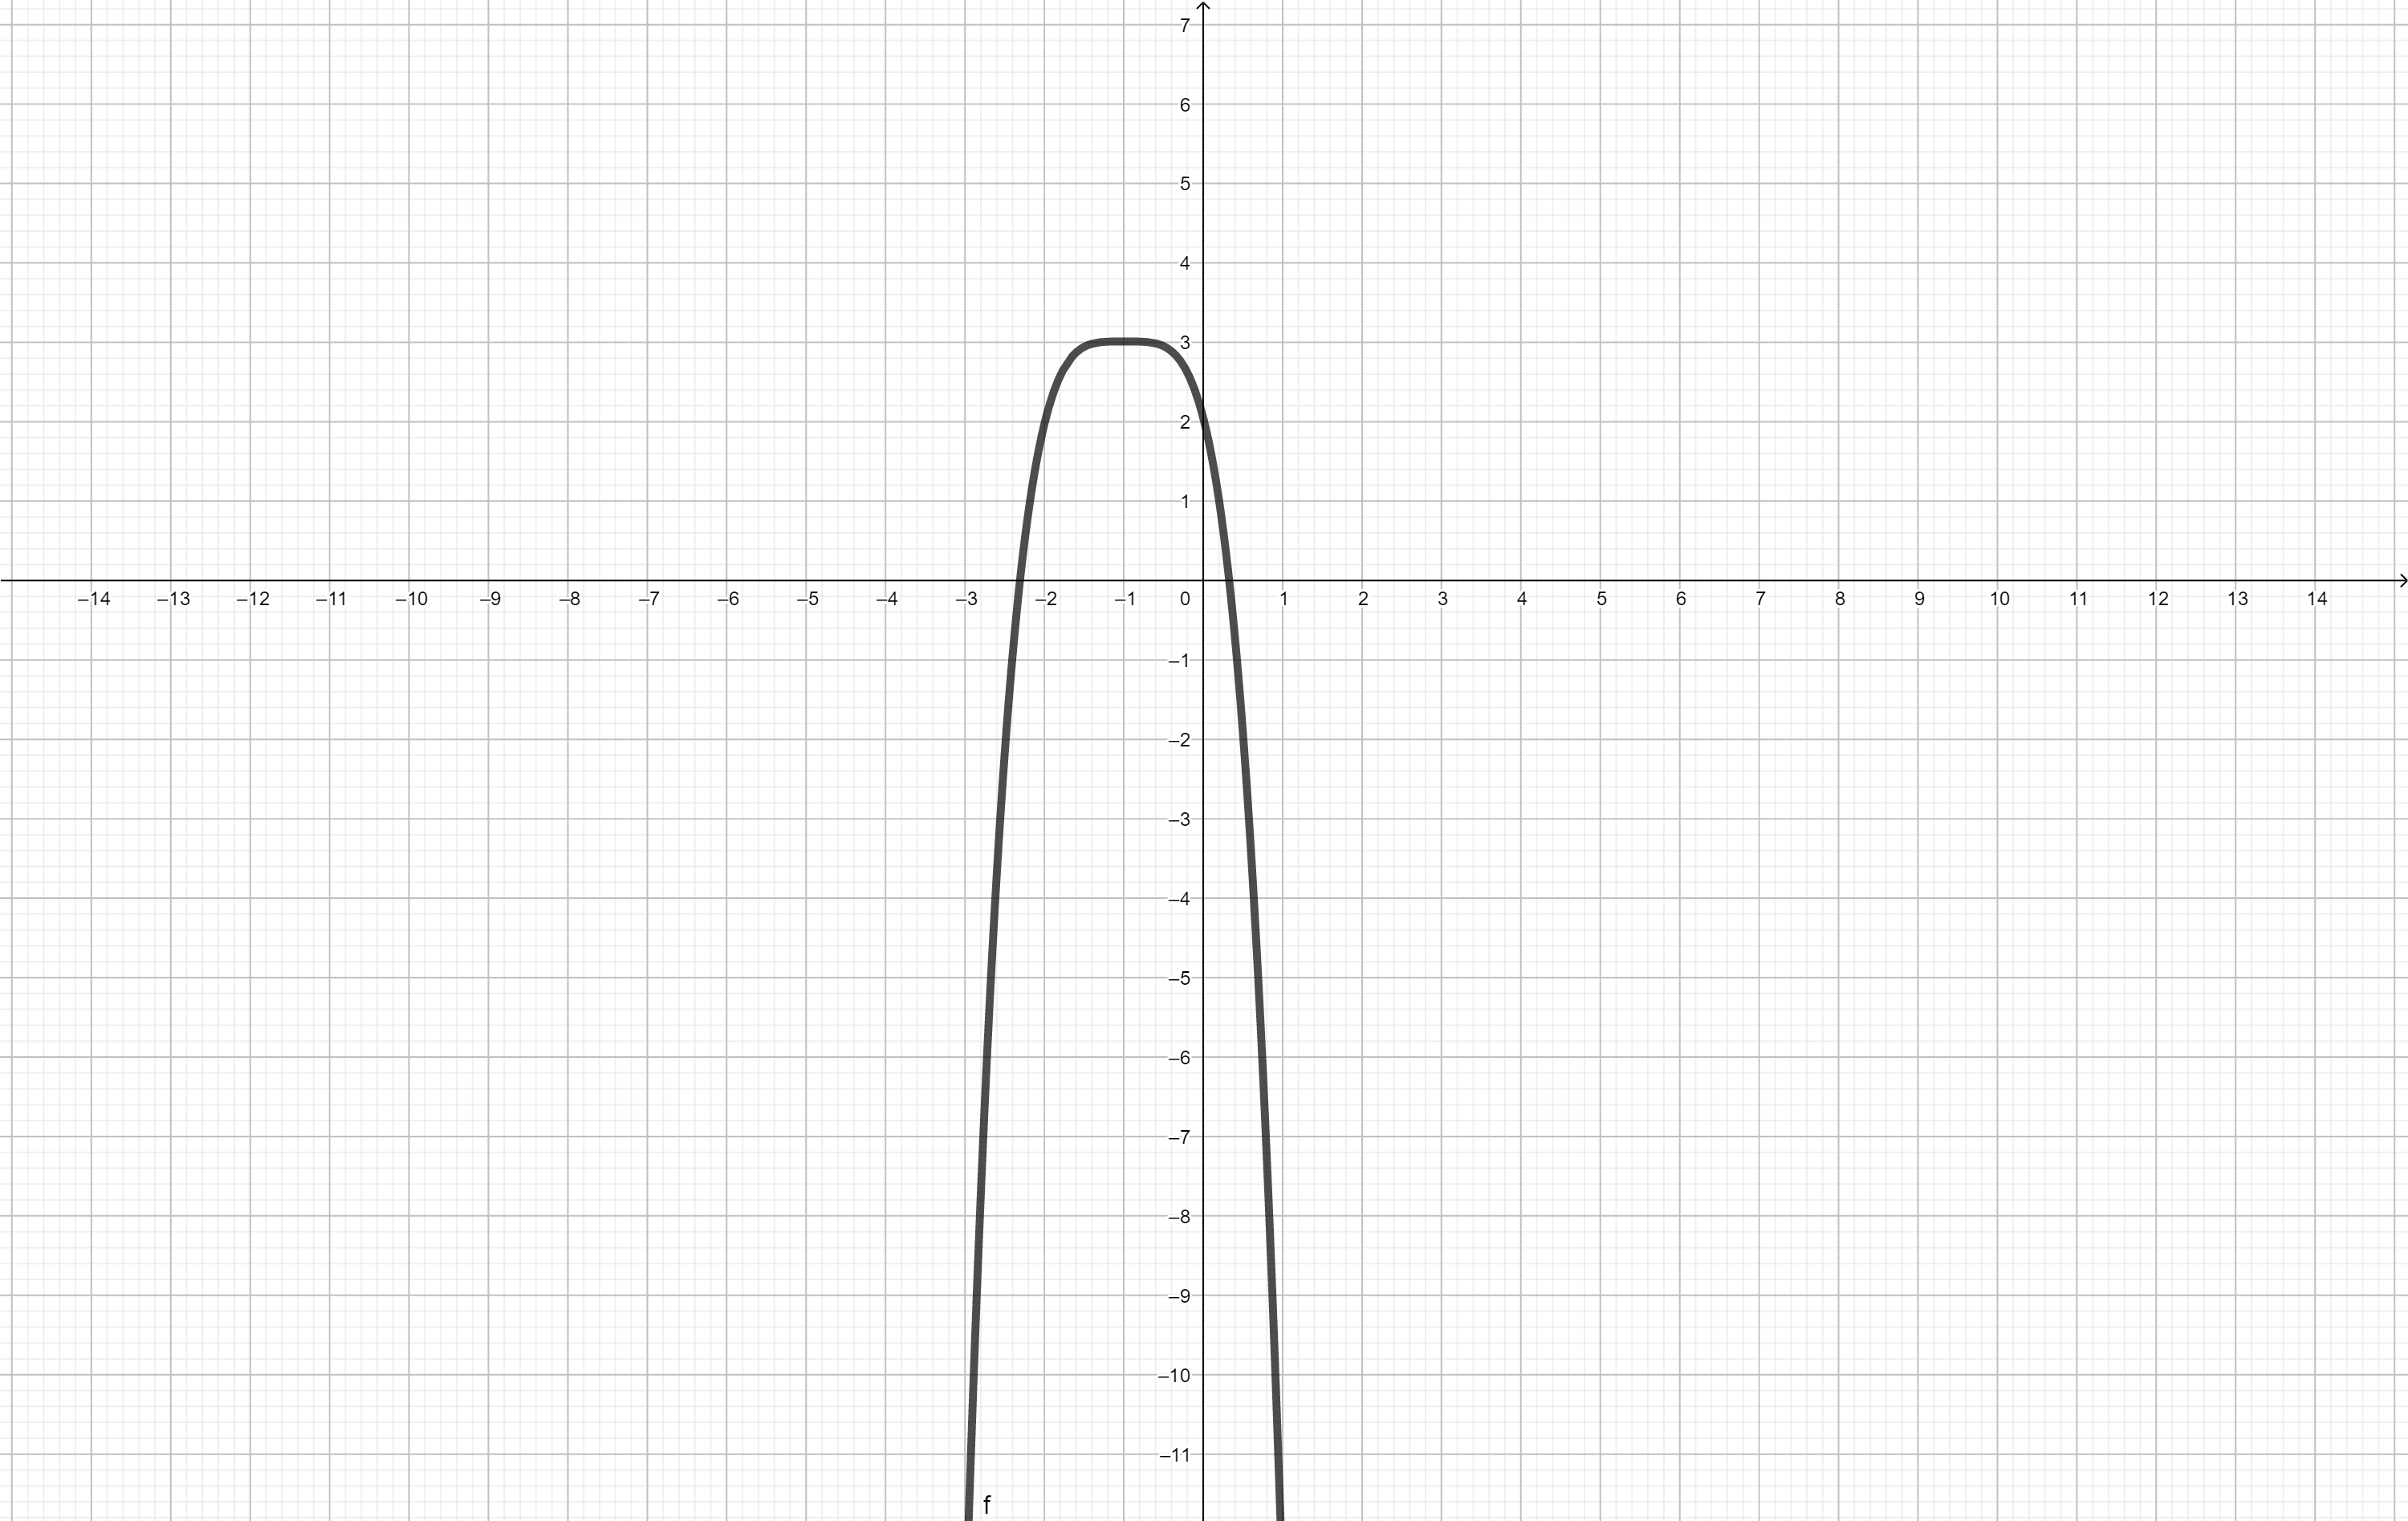
\includegraphics[width=4cm]{Bilder/G48}

\begin{addmargin}[-2cm]{0pt}
Nullstellen:

$x\rightarrow\infty:$

$x\rightarrow-\infty:$
\end{addmargin}

\paragraph{Grad 5:}\textcolor{white}{.}

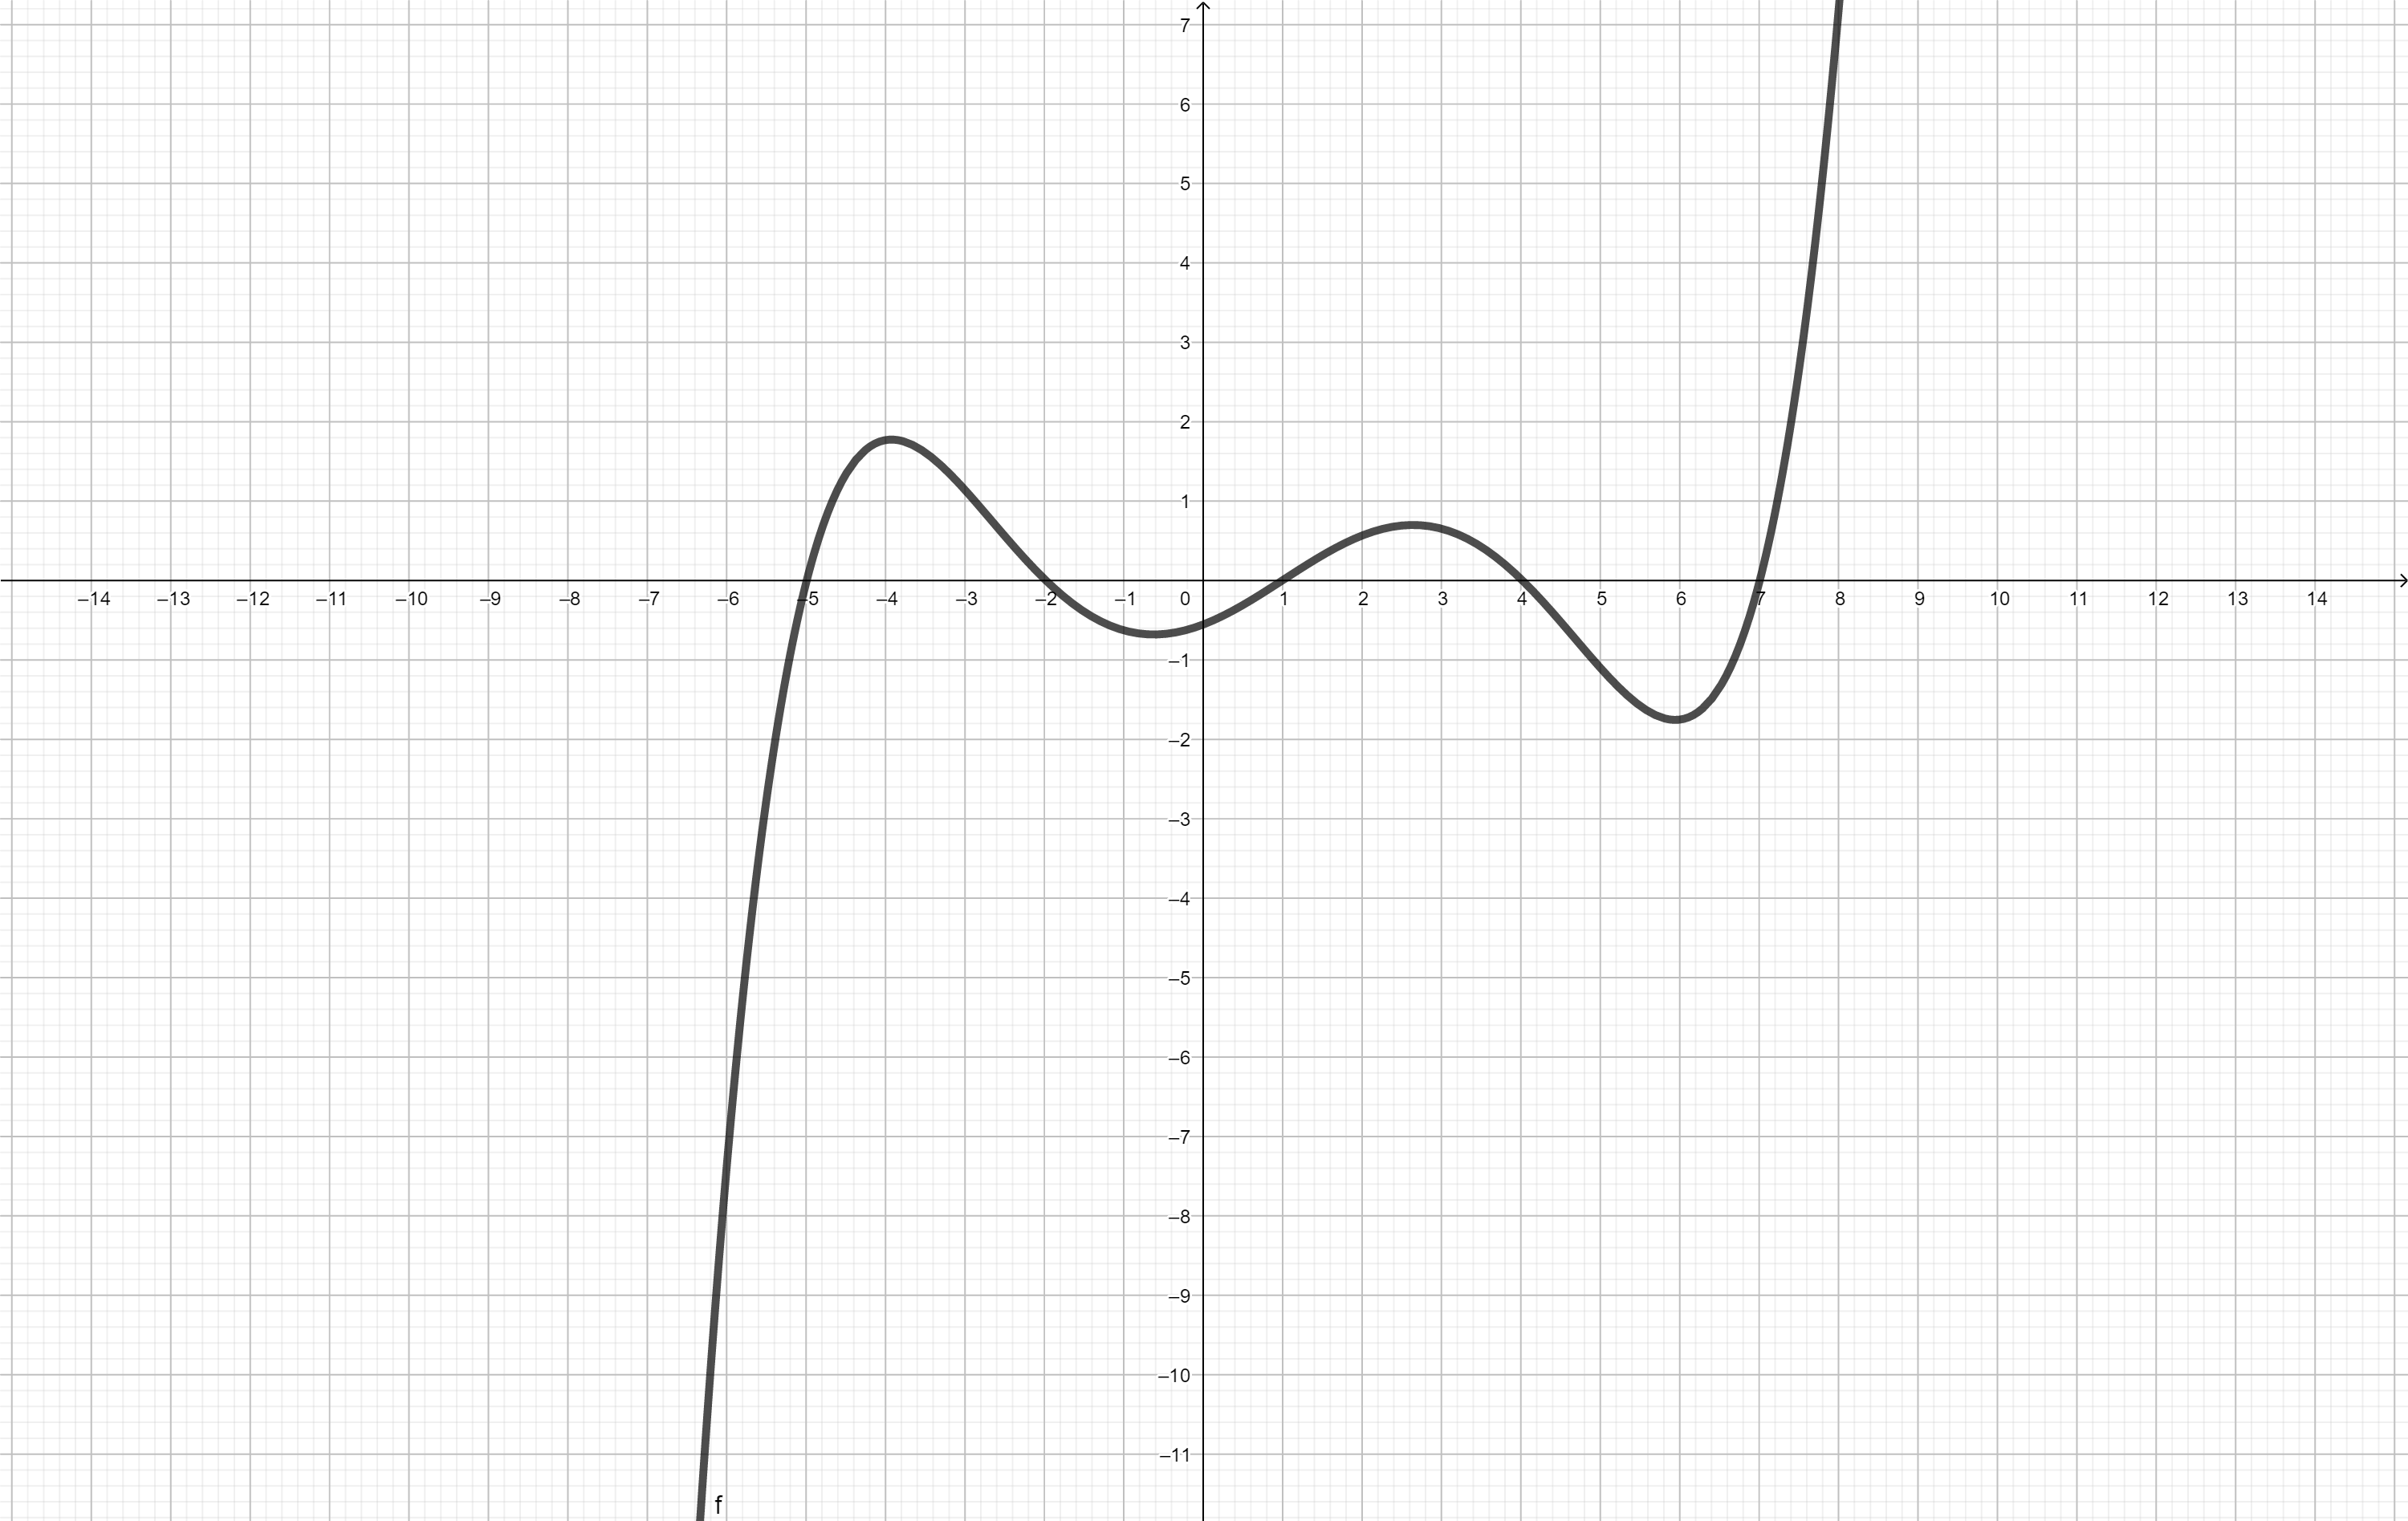
\includegraphics[width=4cm]{Bilder/G51}\hfill
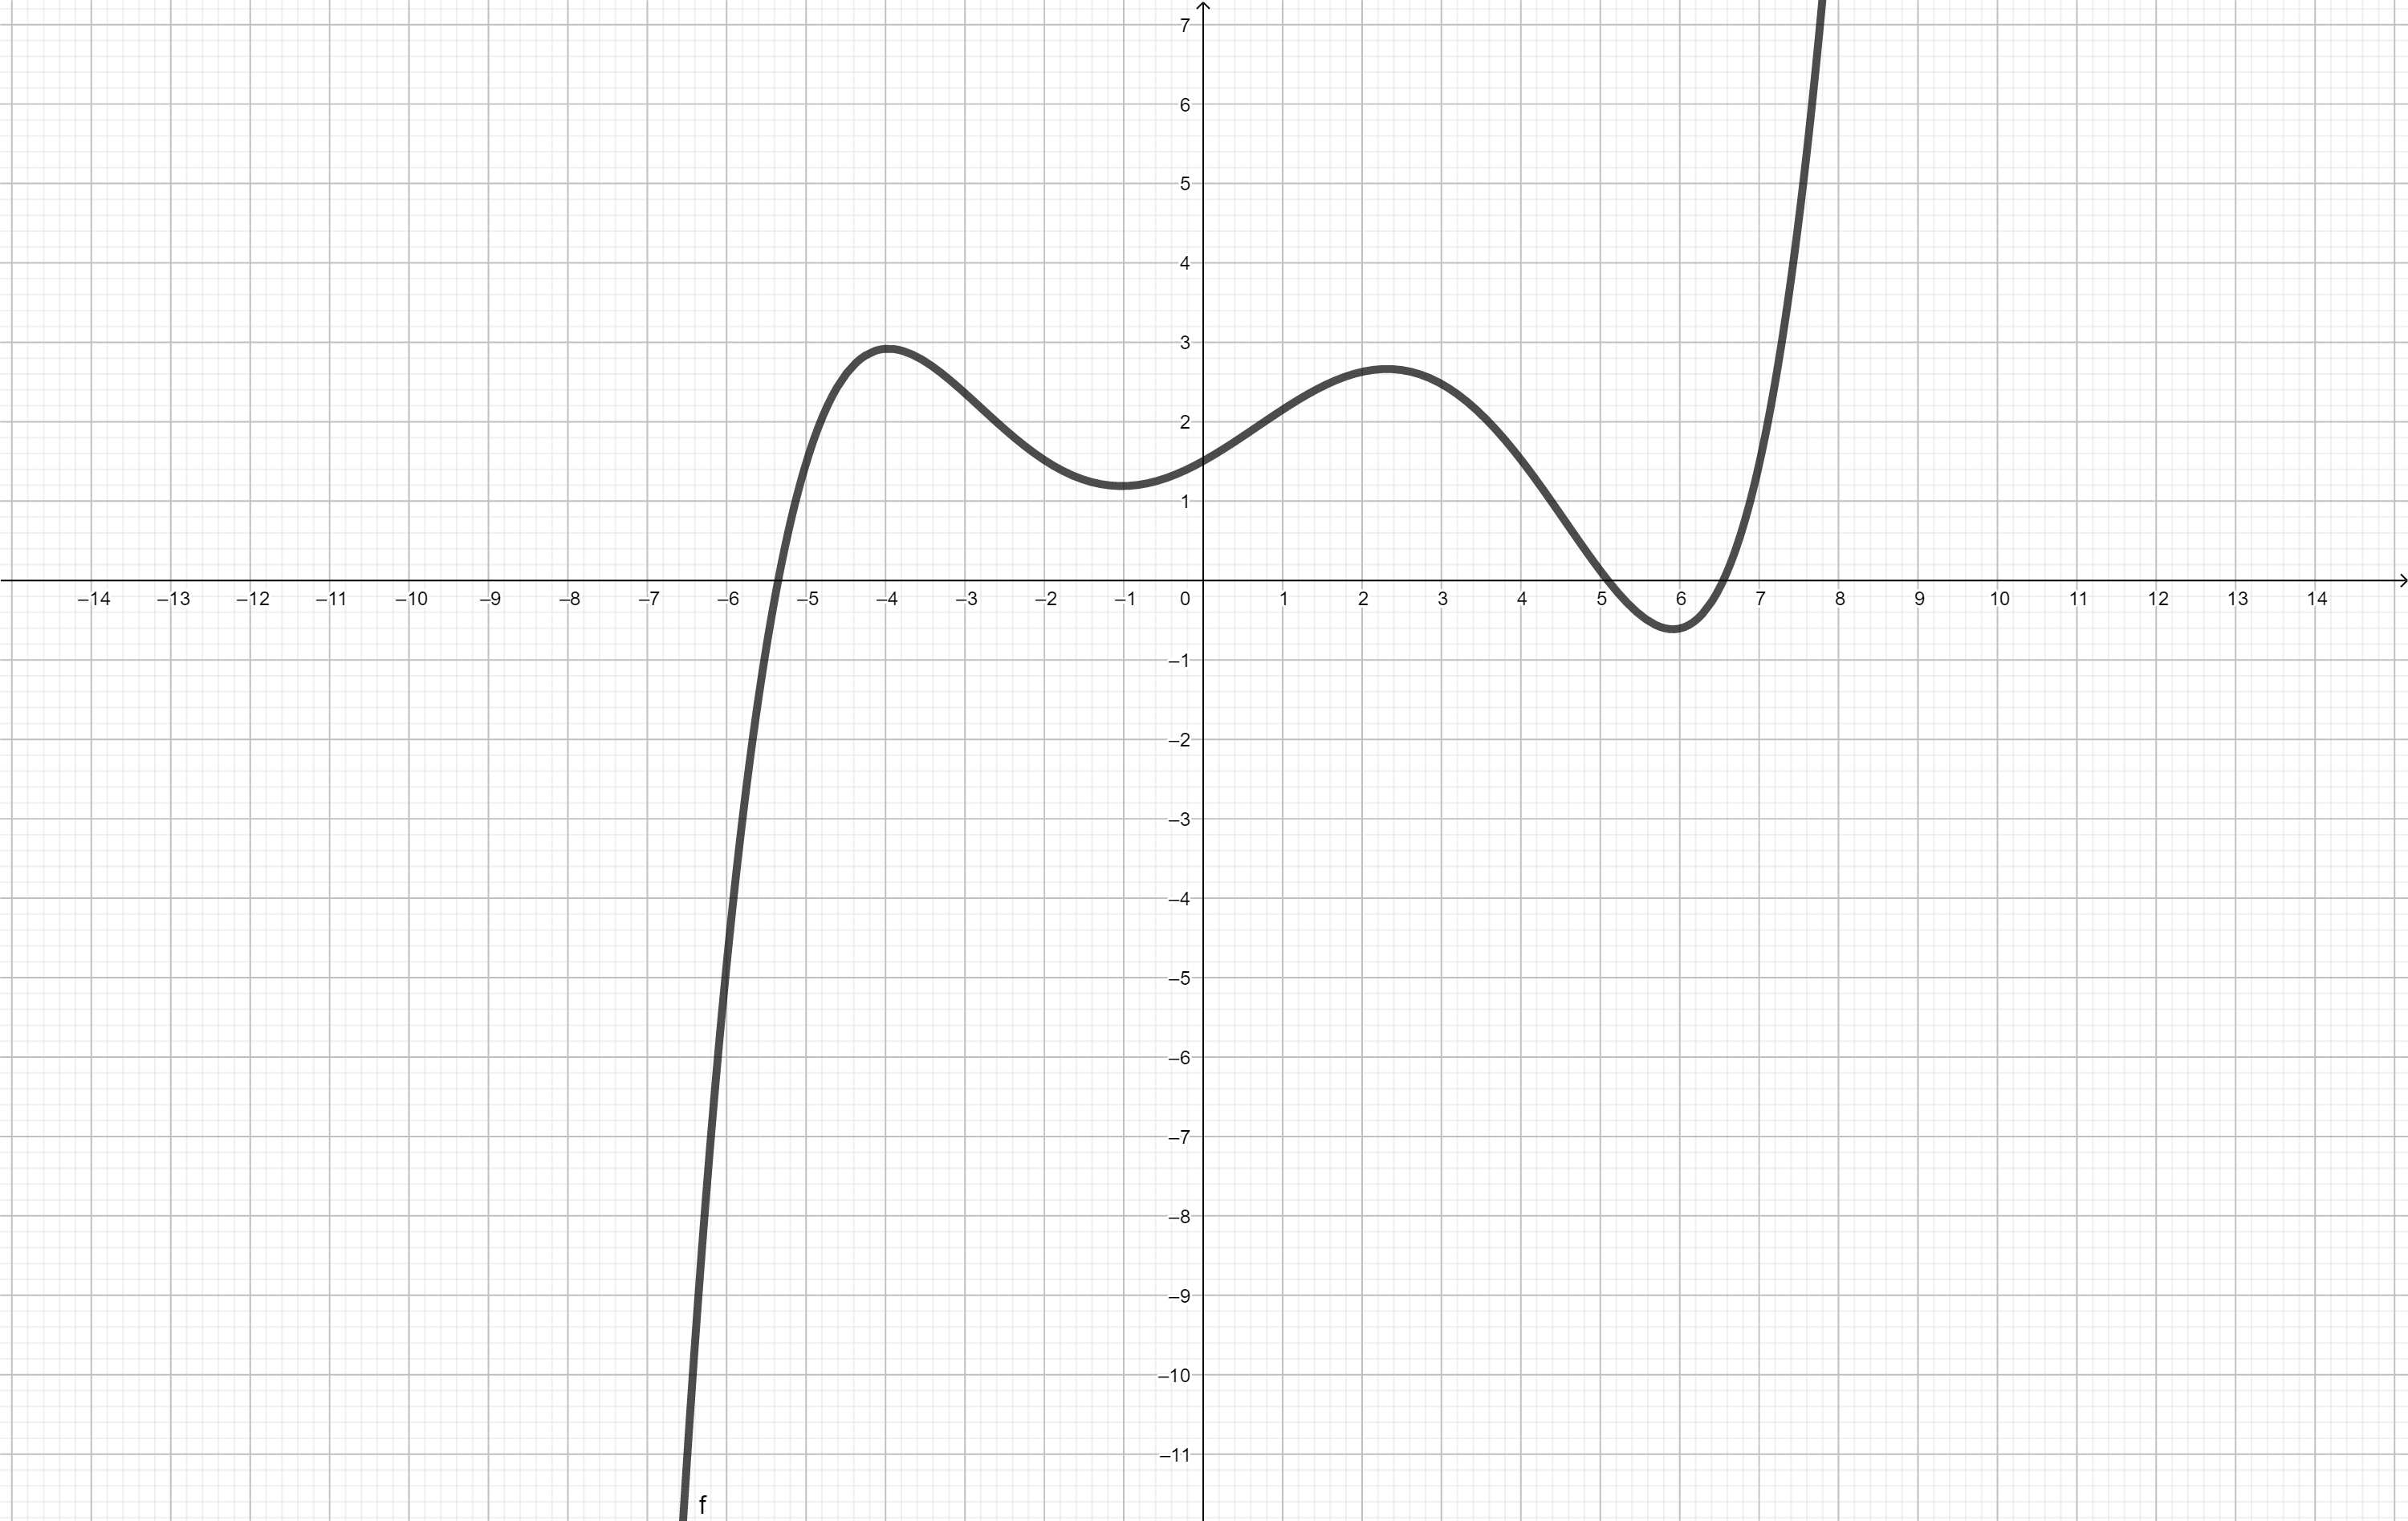
\includegraphics[width=4cm]{Bilder/G52}\hfill
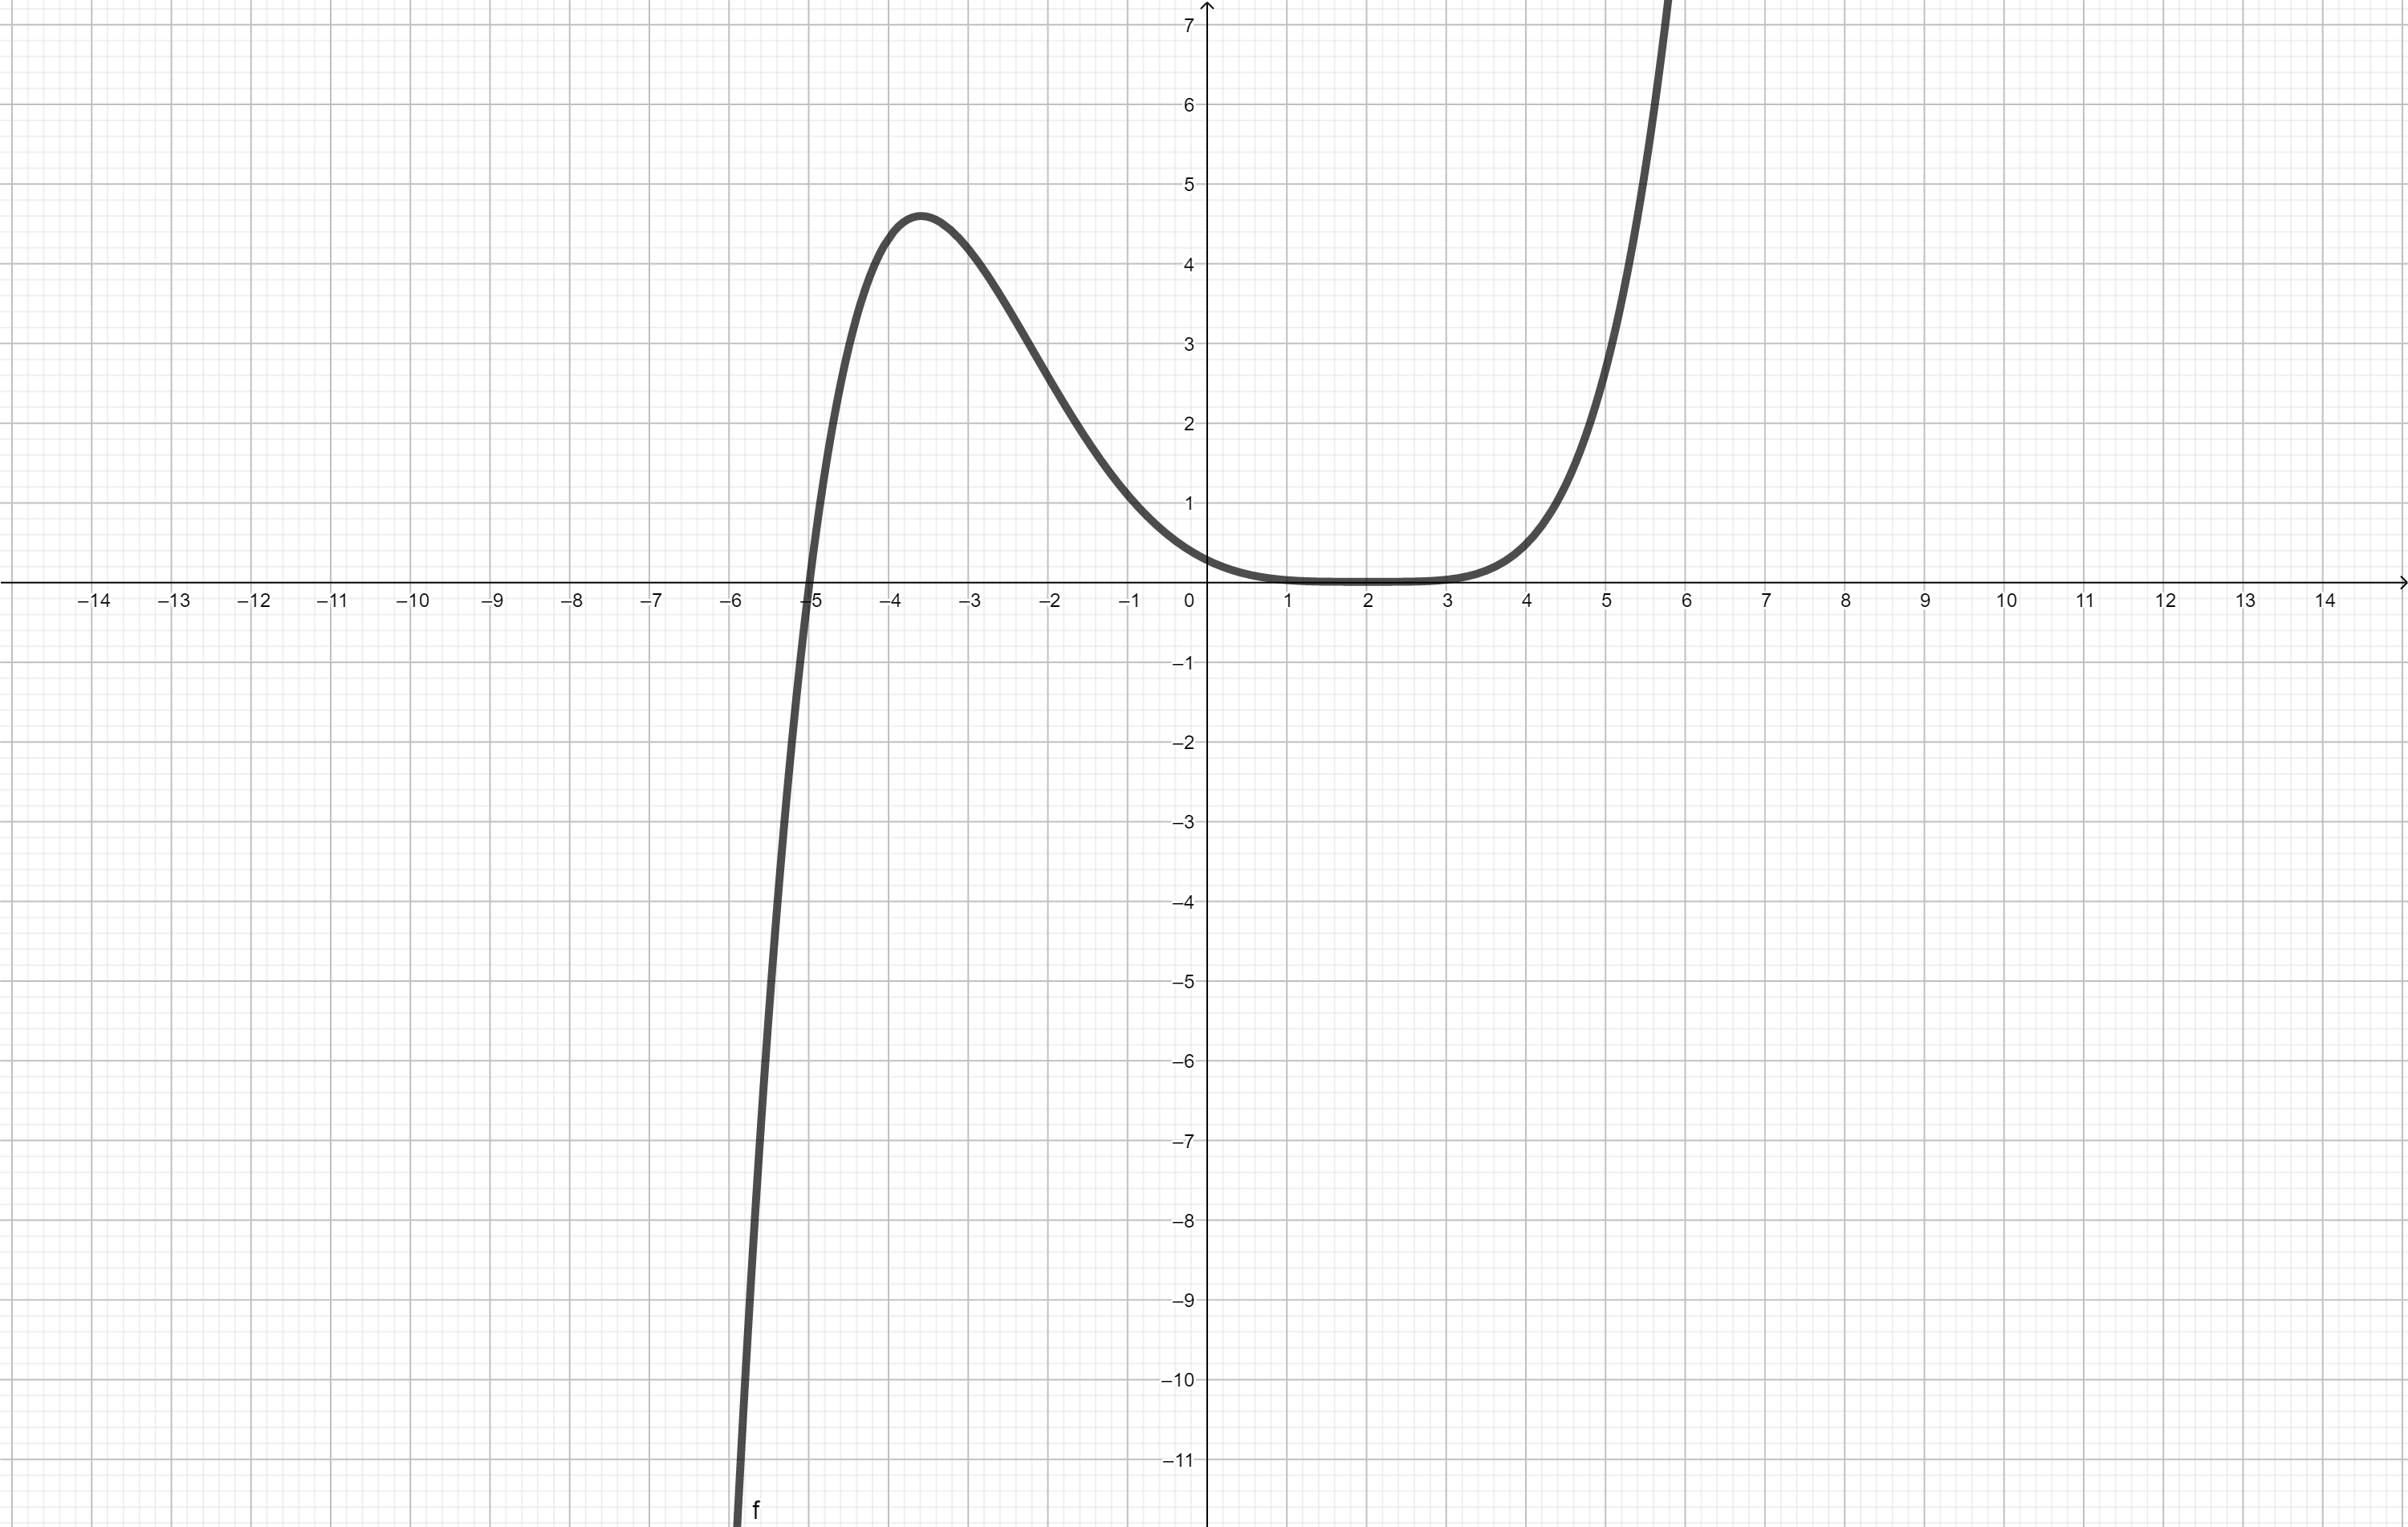
\includegraphics[width=4cm]{Bilder/G53}\hfill
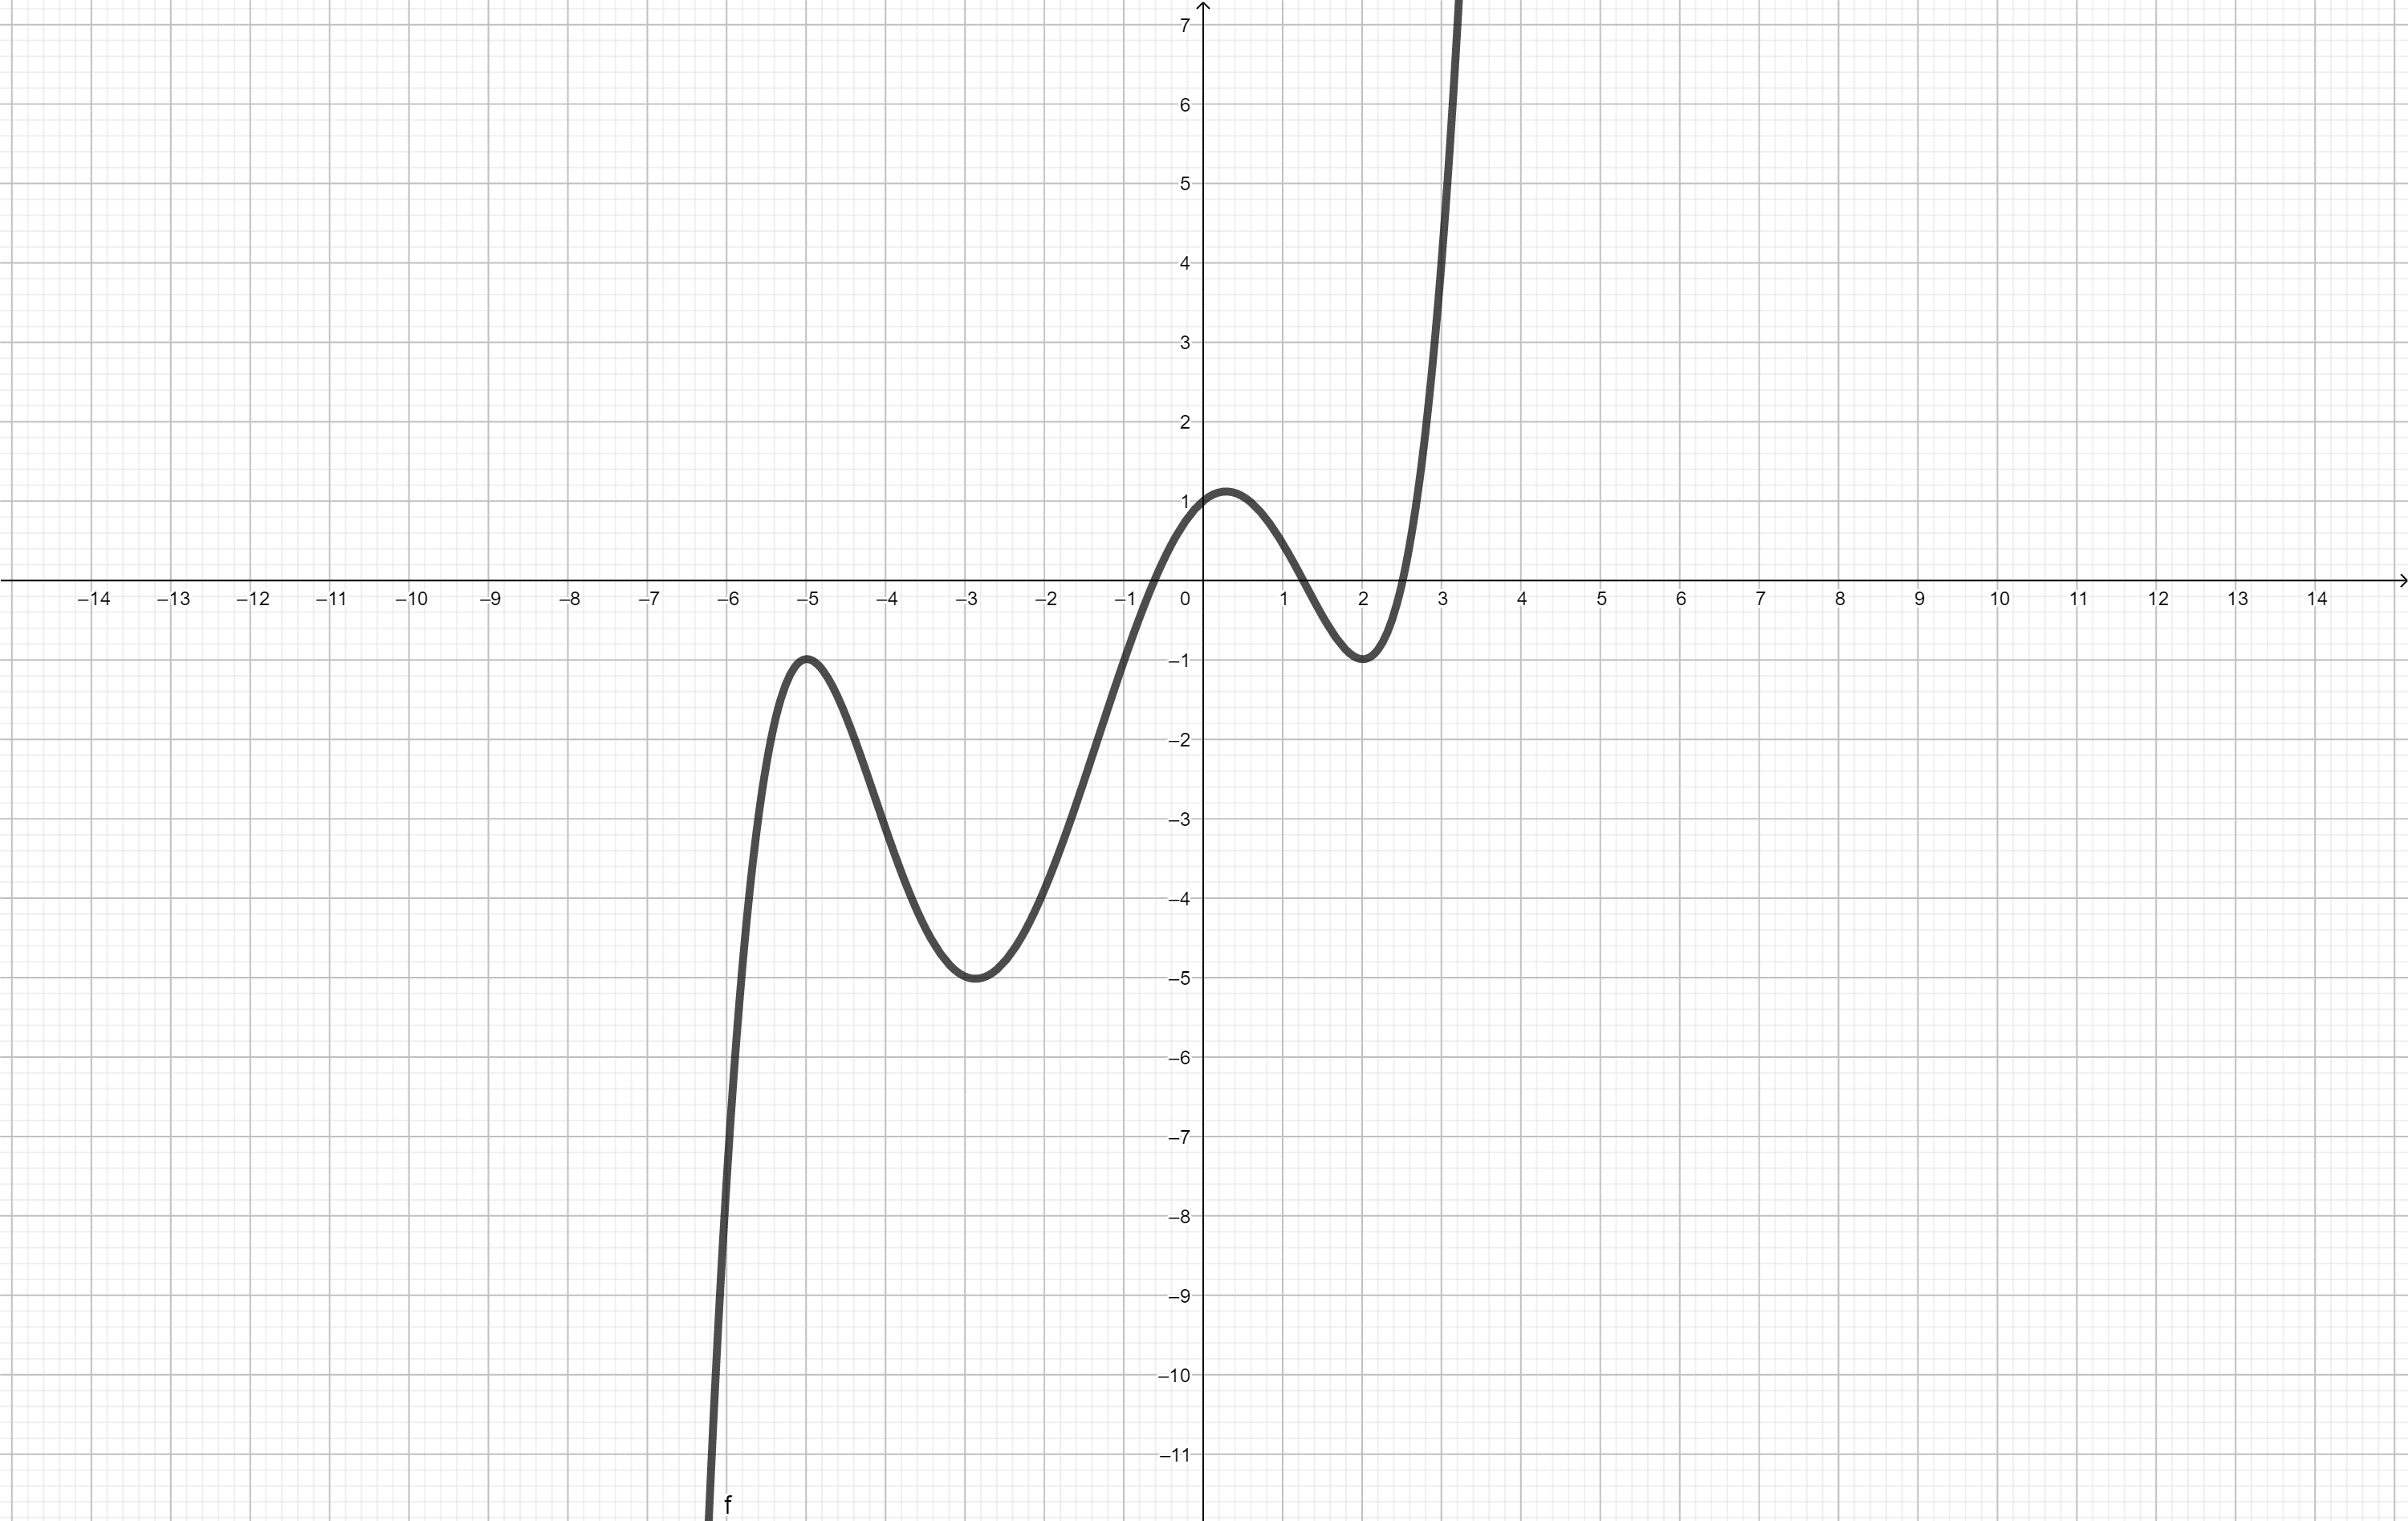
\includegraphics[width=4cm]{Bilder/G54}

\begin{addmargin}[-2cm]{0pt}
Nullstellen:

$x\rightarrow\infty:$

$x\rightarrow-\infty:$
\end{addmargin}

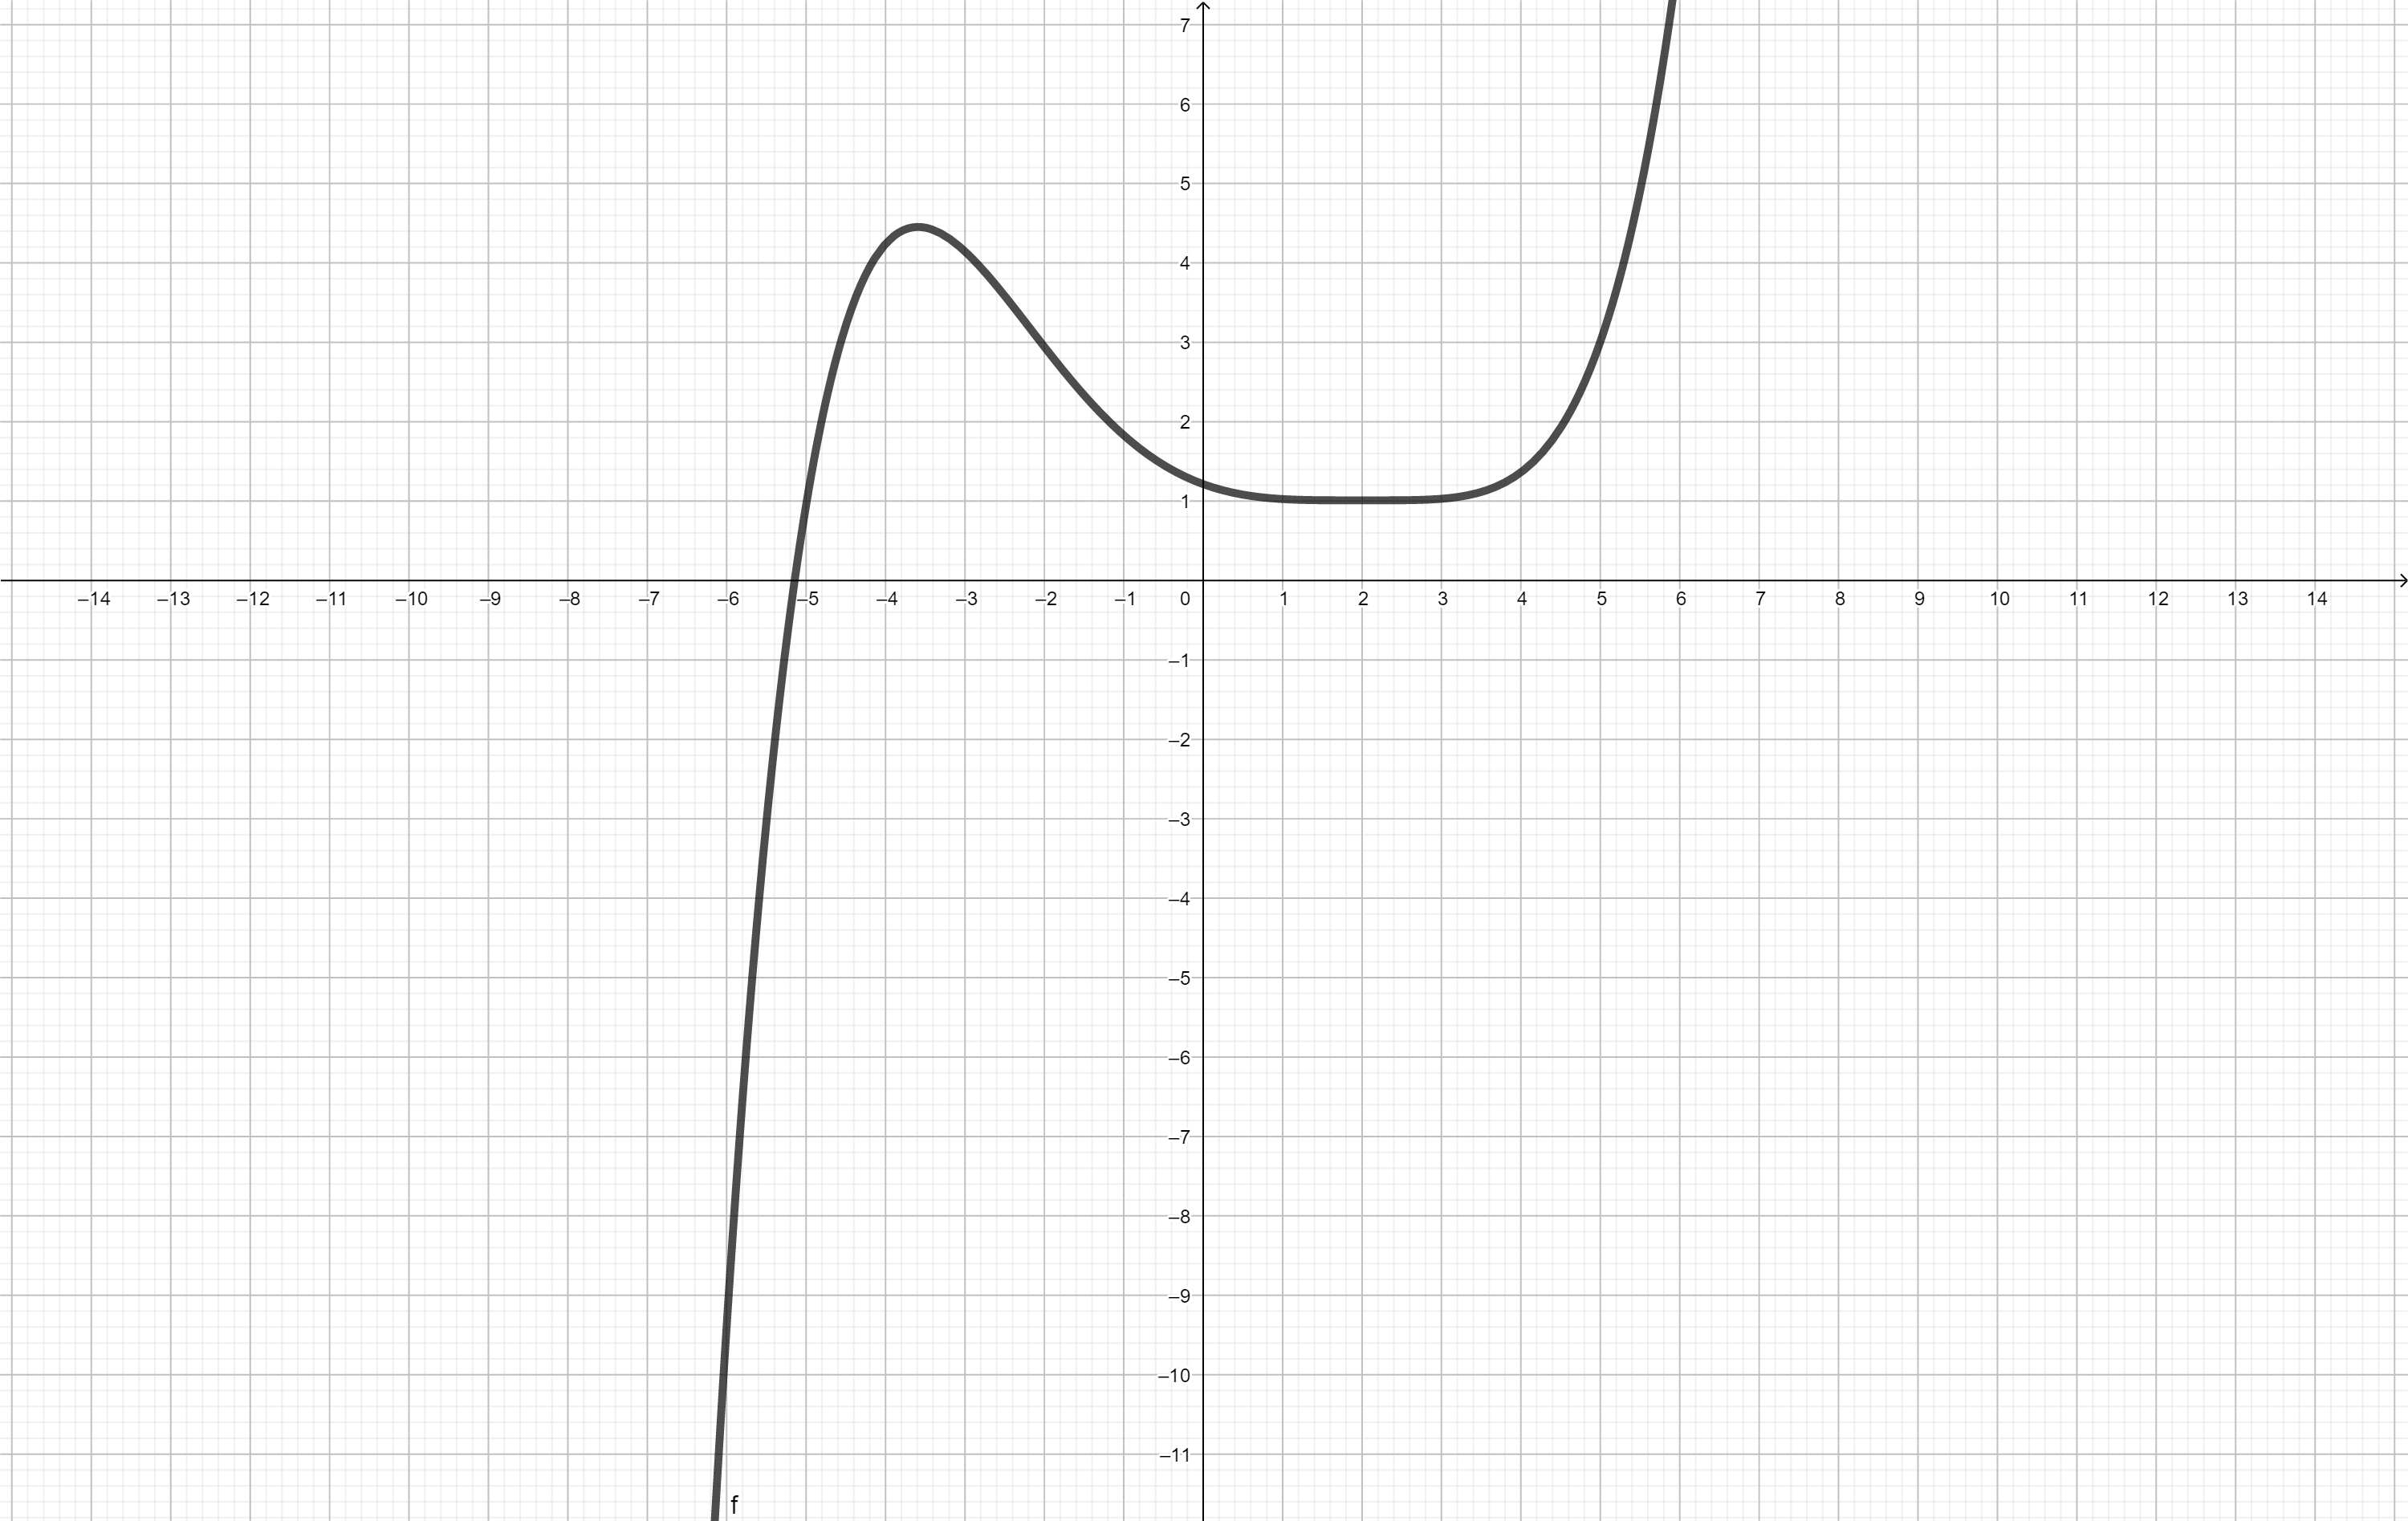
\includegraphics[width=4cm]{Bilder/G55}\hfill
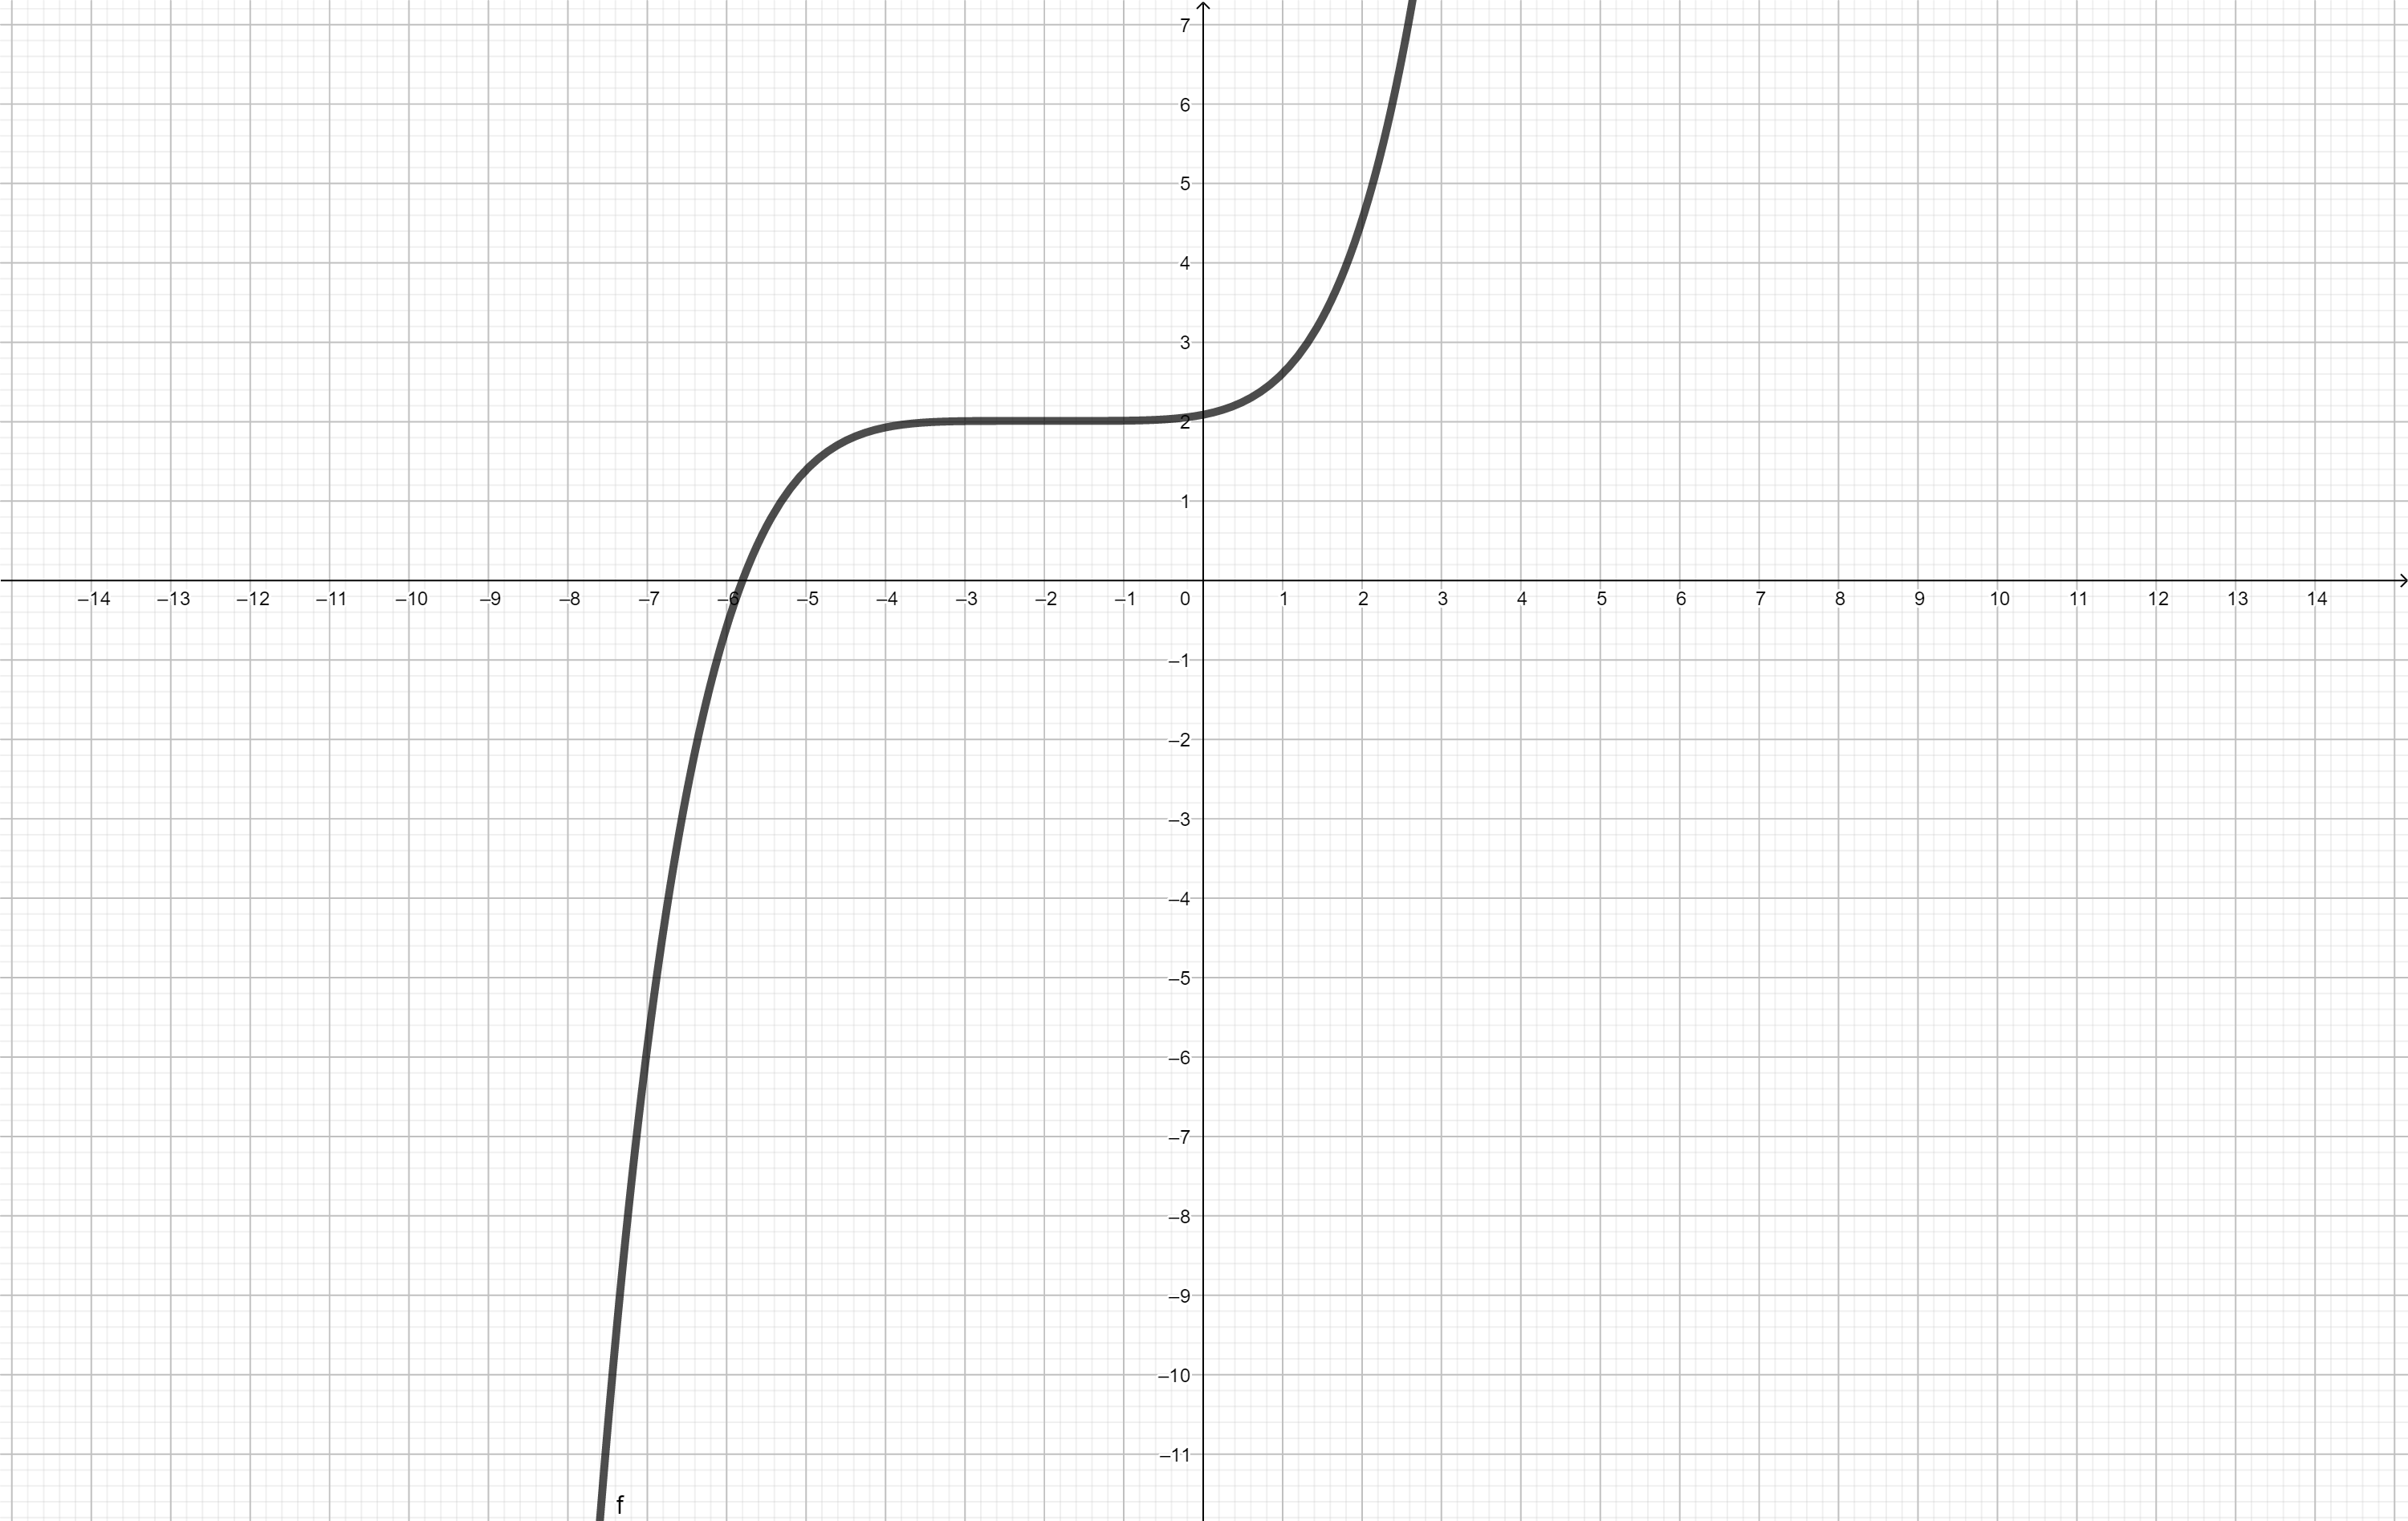
\includegraphics[width=4cm]{Bilder/G56}\hfill
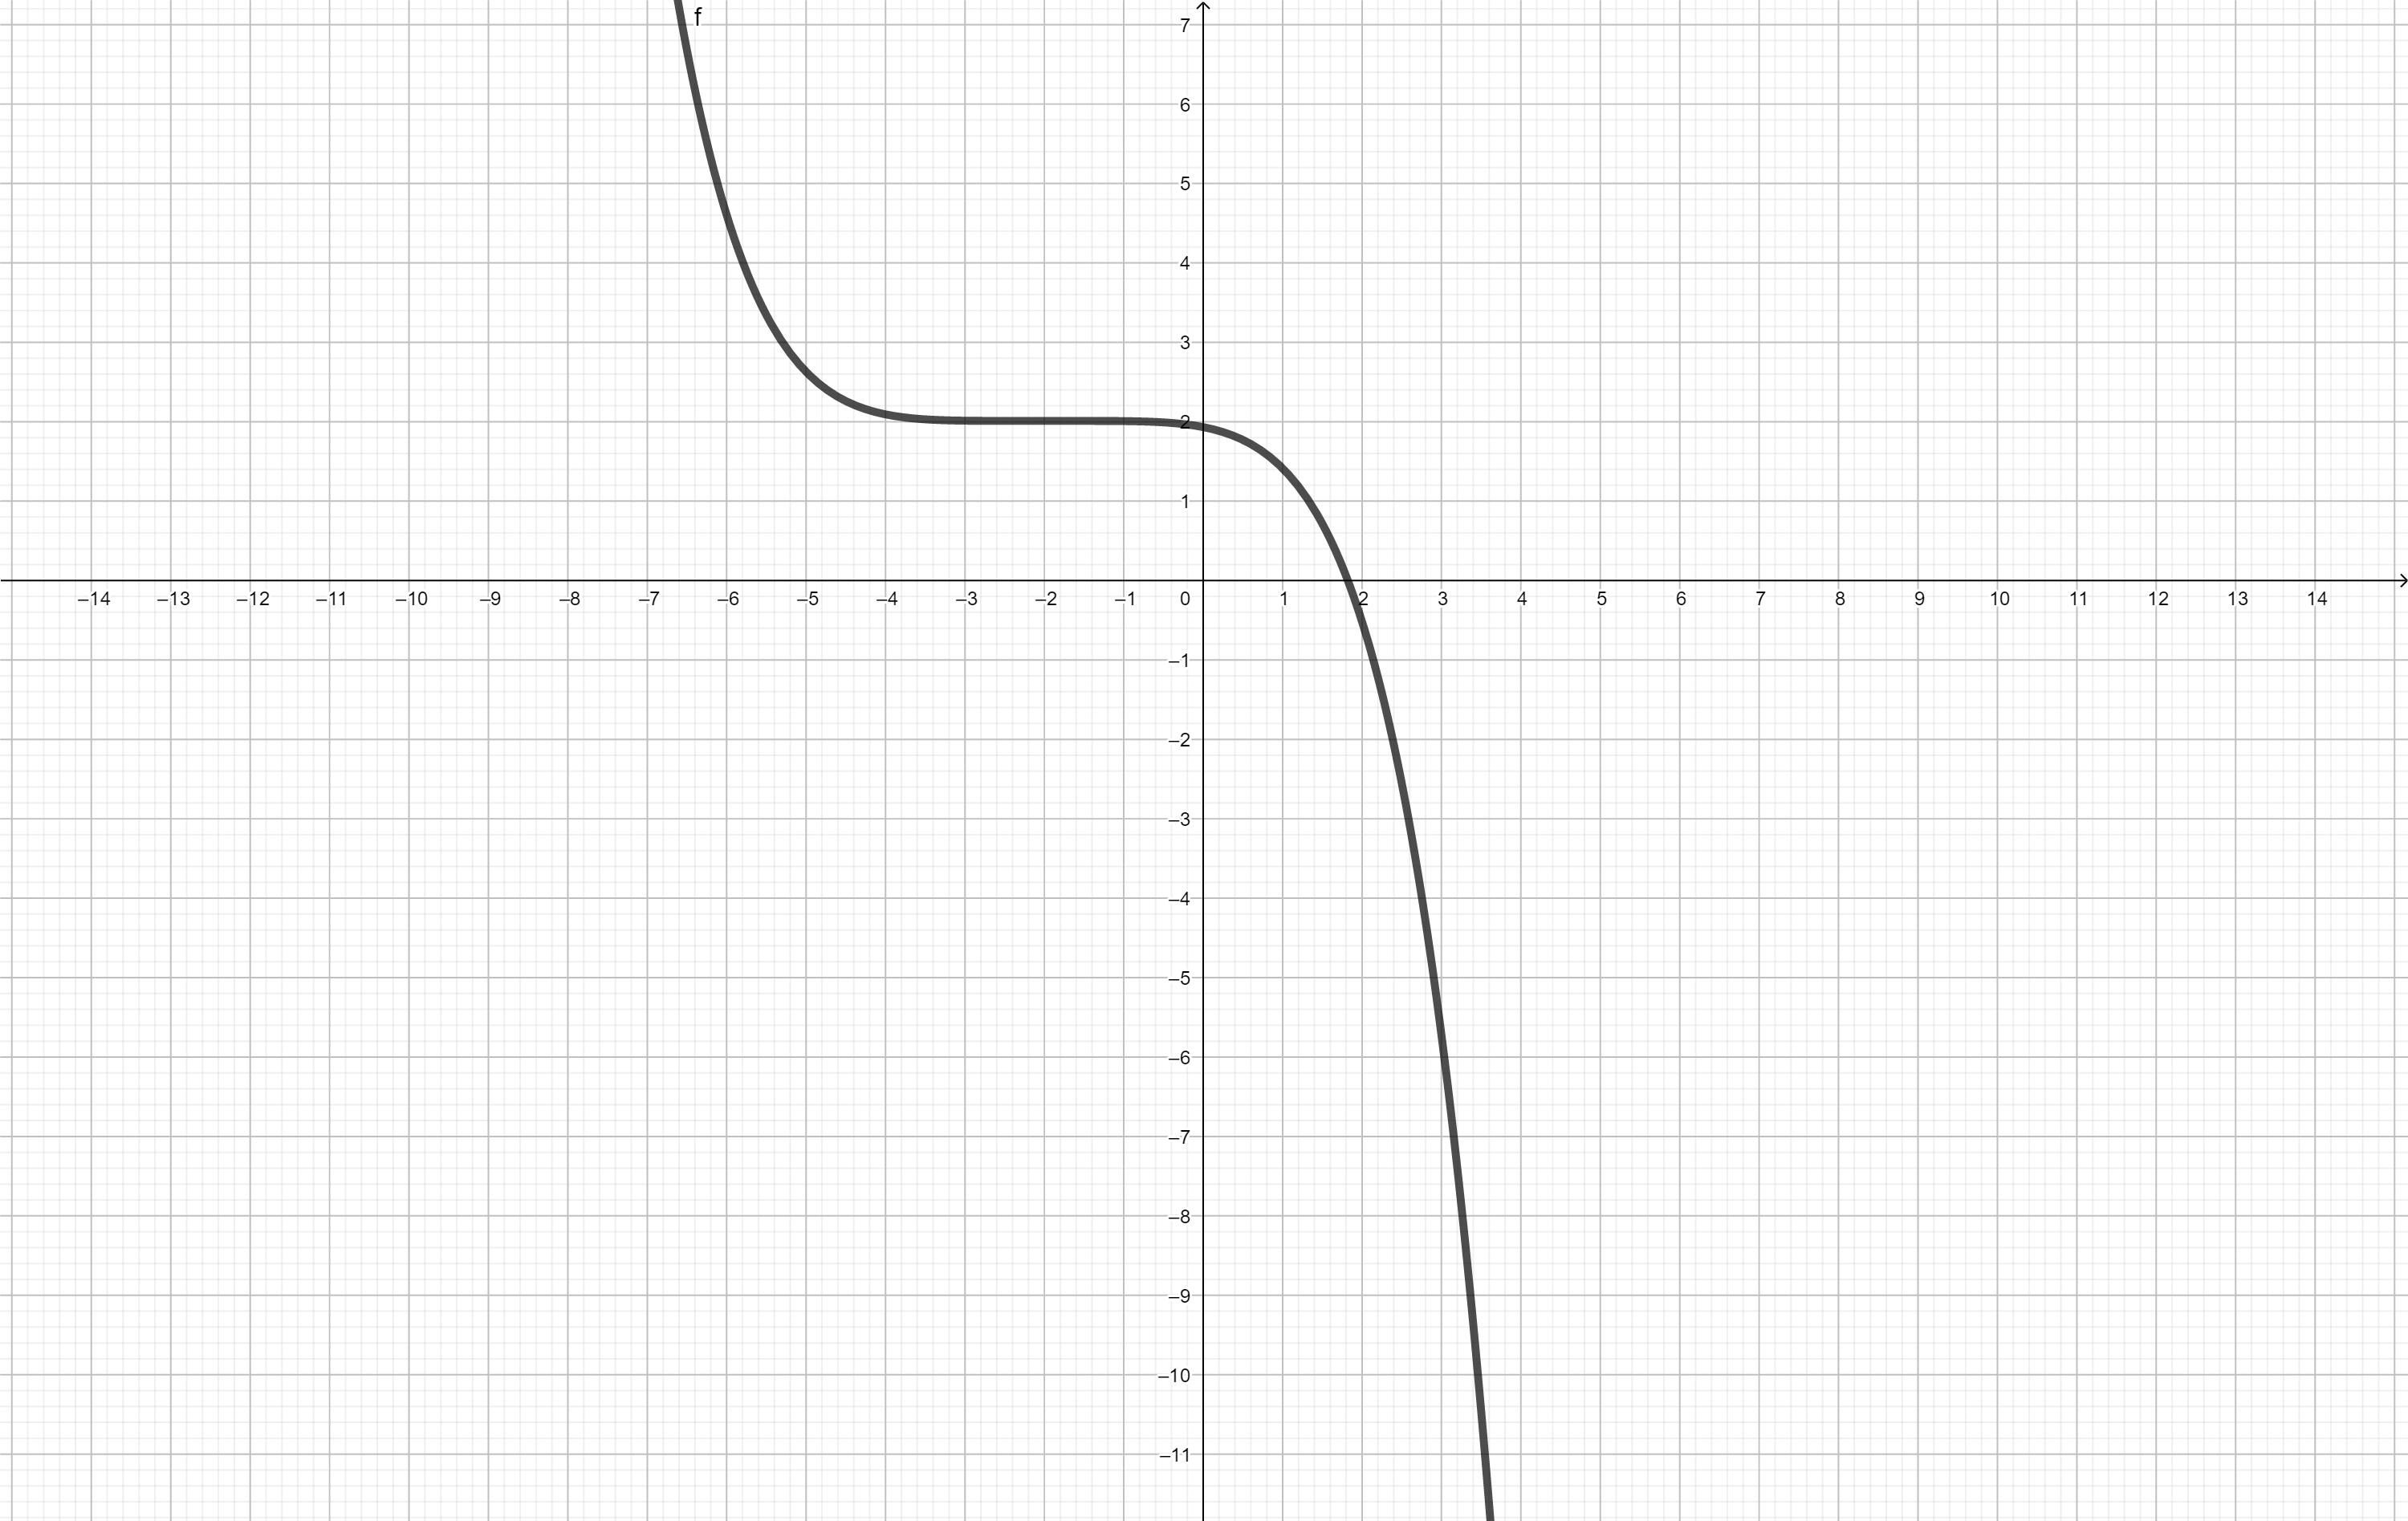
\includegraphics[width=4cm]{Bilder/G57}\hfill
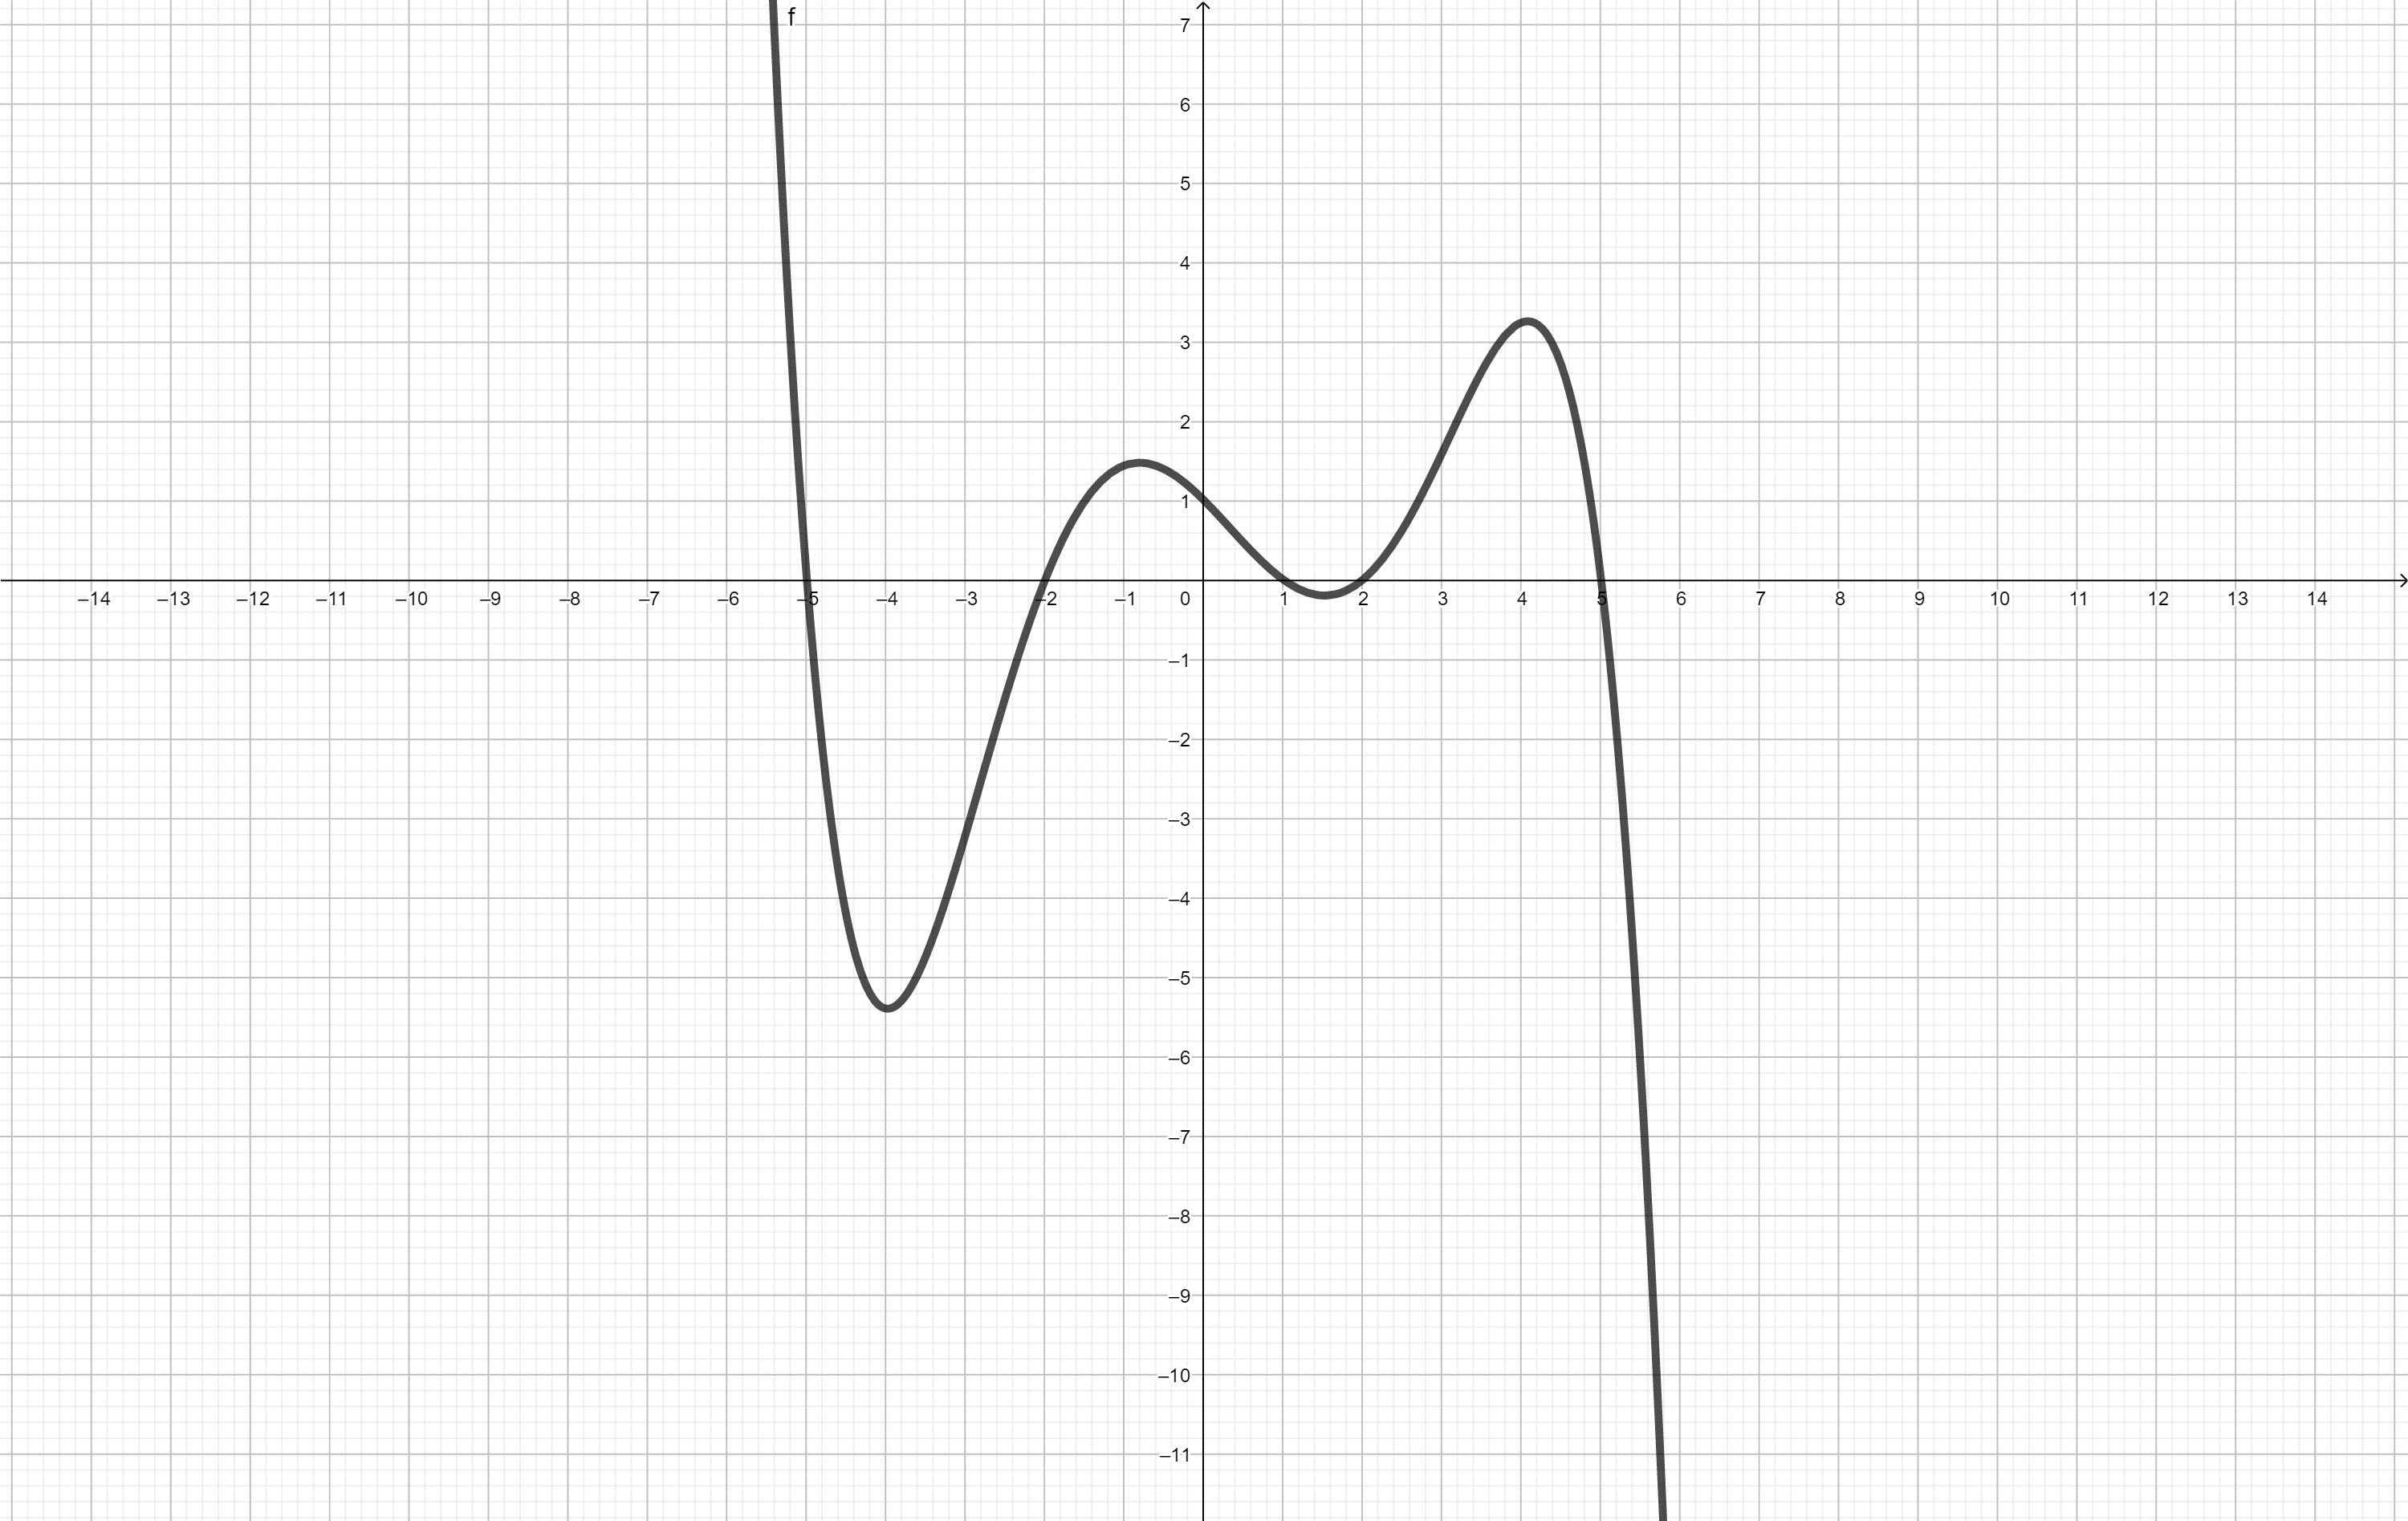
\includegraphics[width=4cm]{Bilder/G58}

\begin{addmargin}[-2cm]{0pt}
Nullstellen:

$x\rightarrow\infty:$

$x\rightarrow-\infty:$
\end{addmargin}

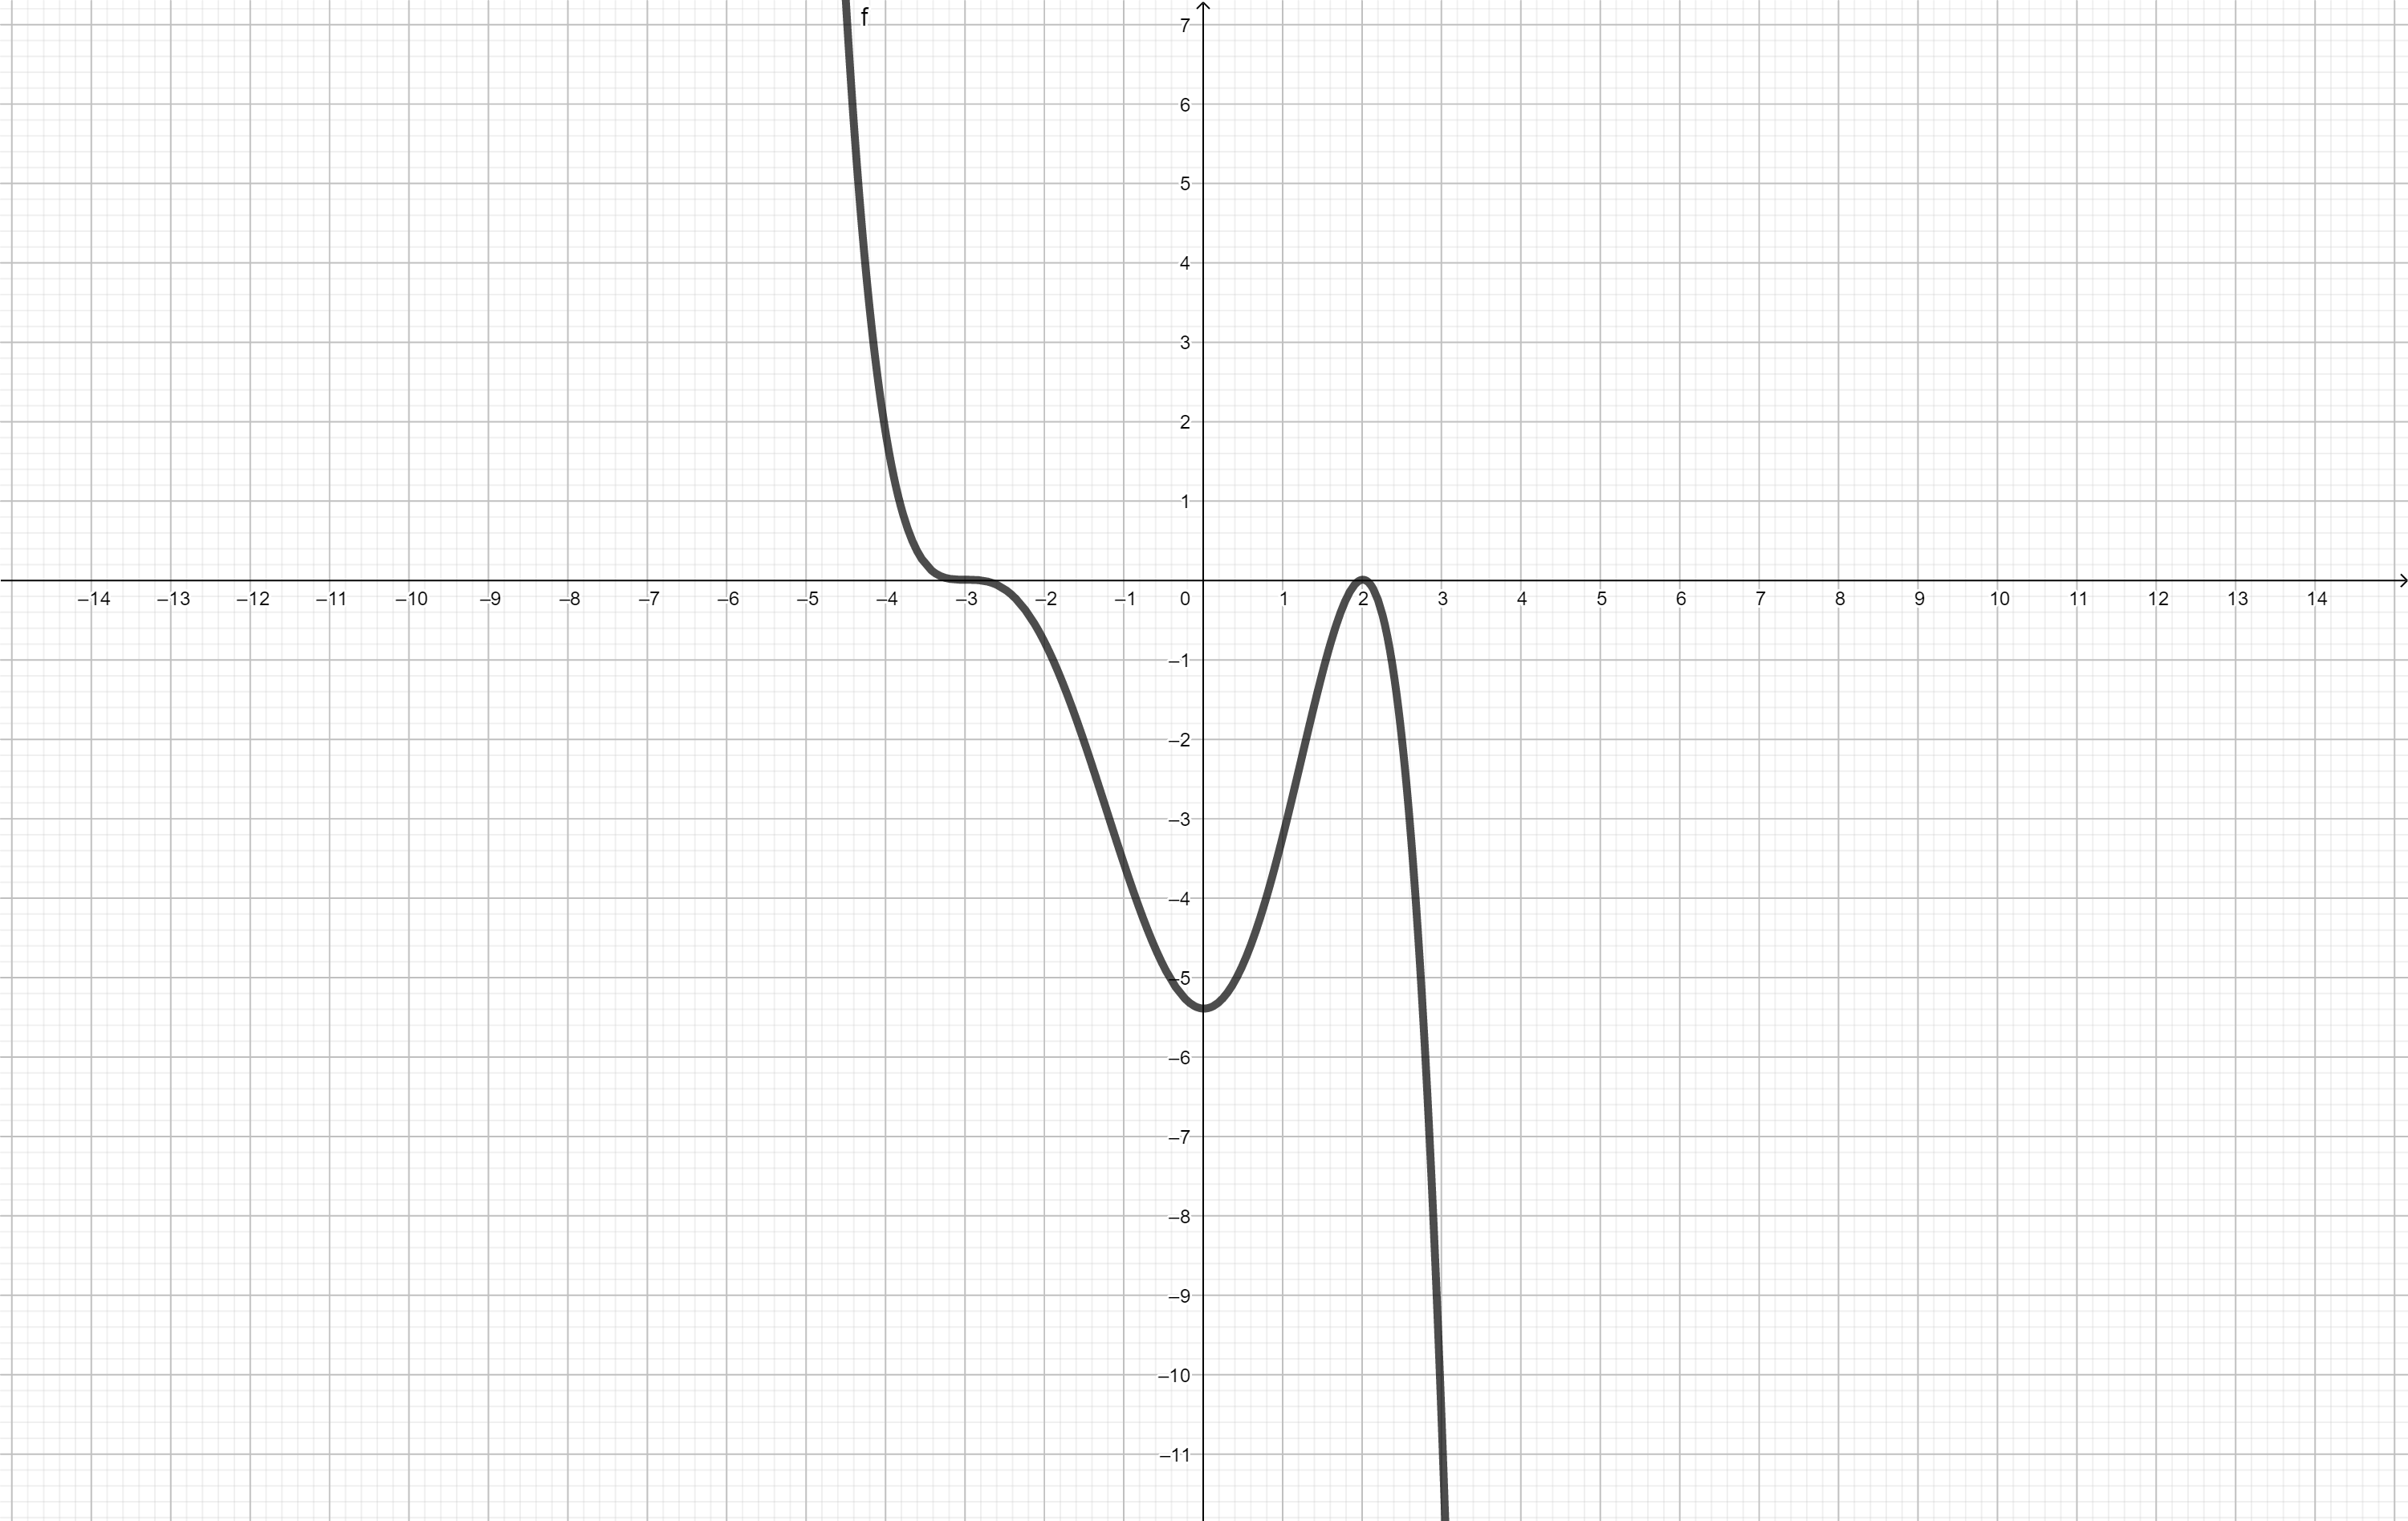
\includegraphics[width=4cm]{Bilder/G59}\hfill
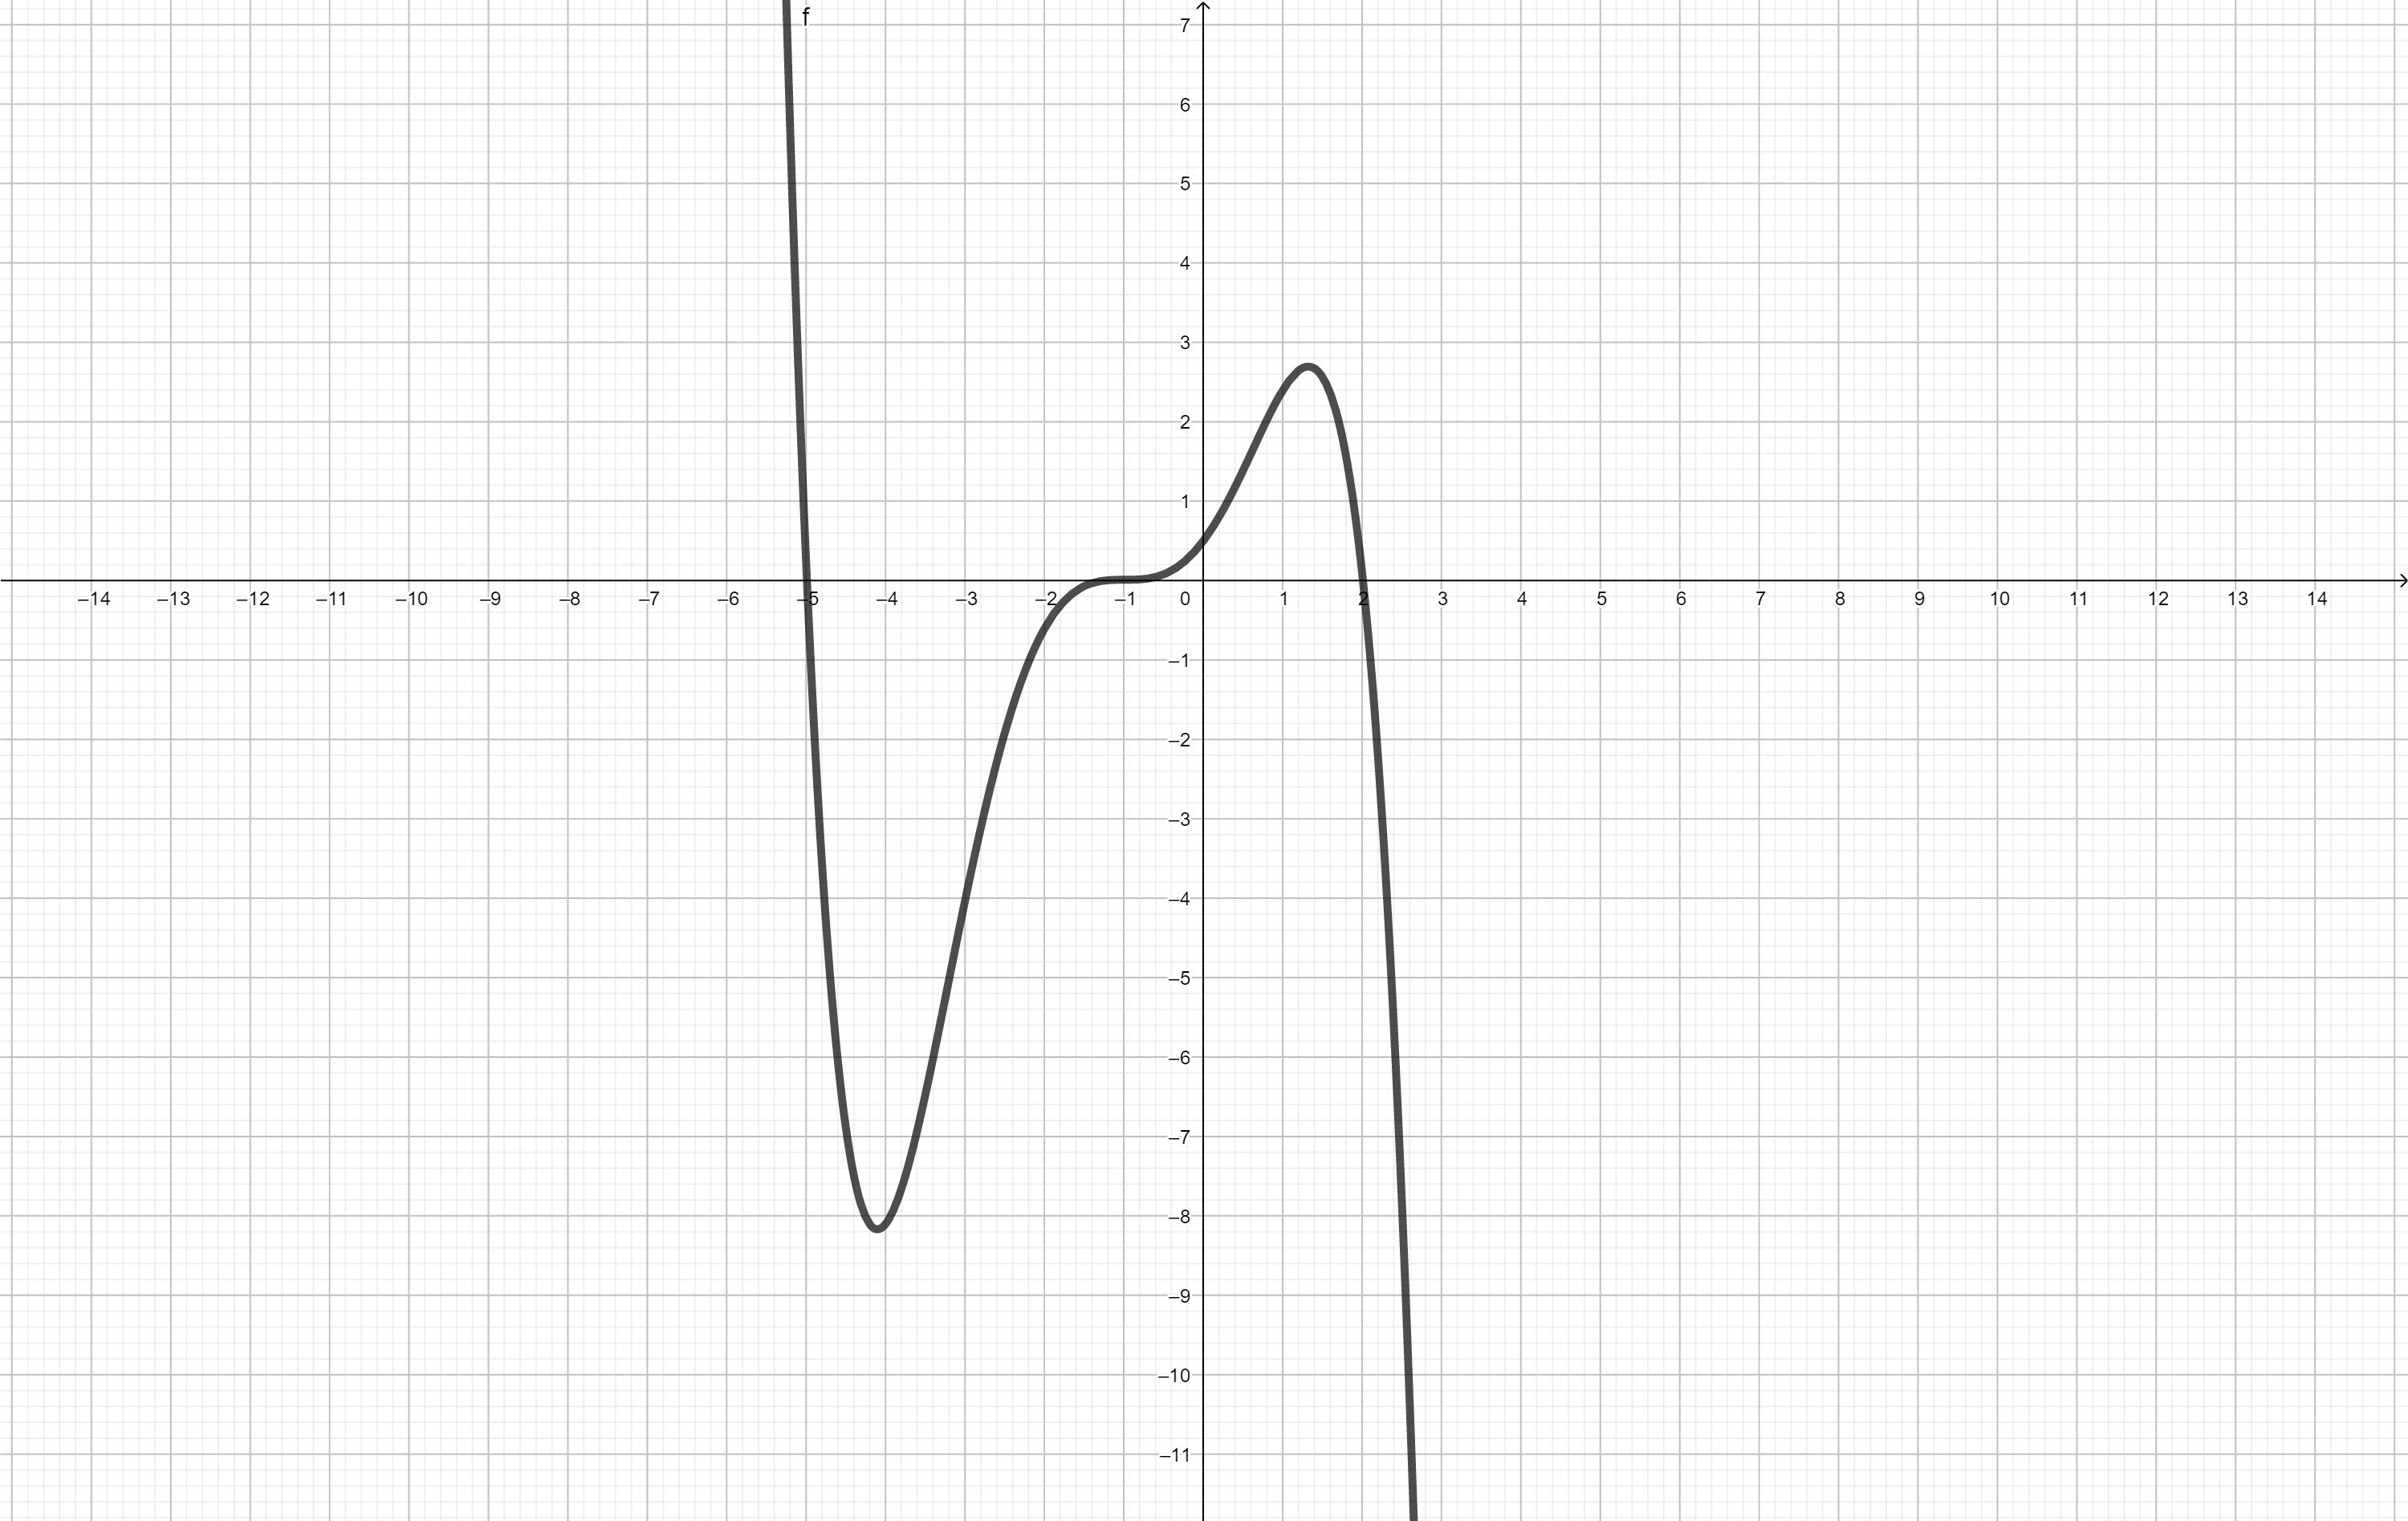
\includegraphics[width=4cm]{Bilder/G510}\hfill
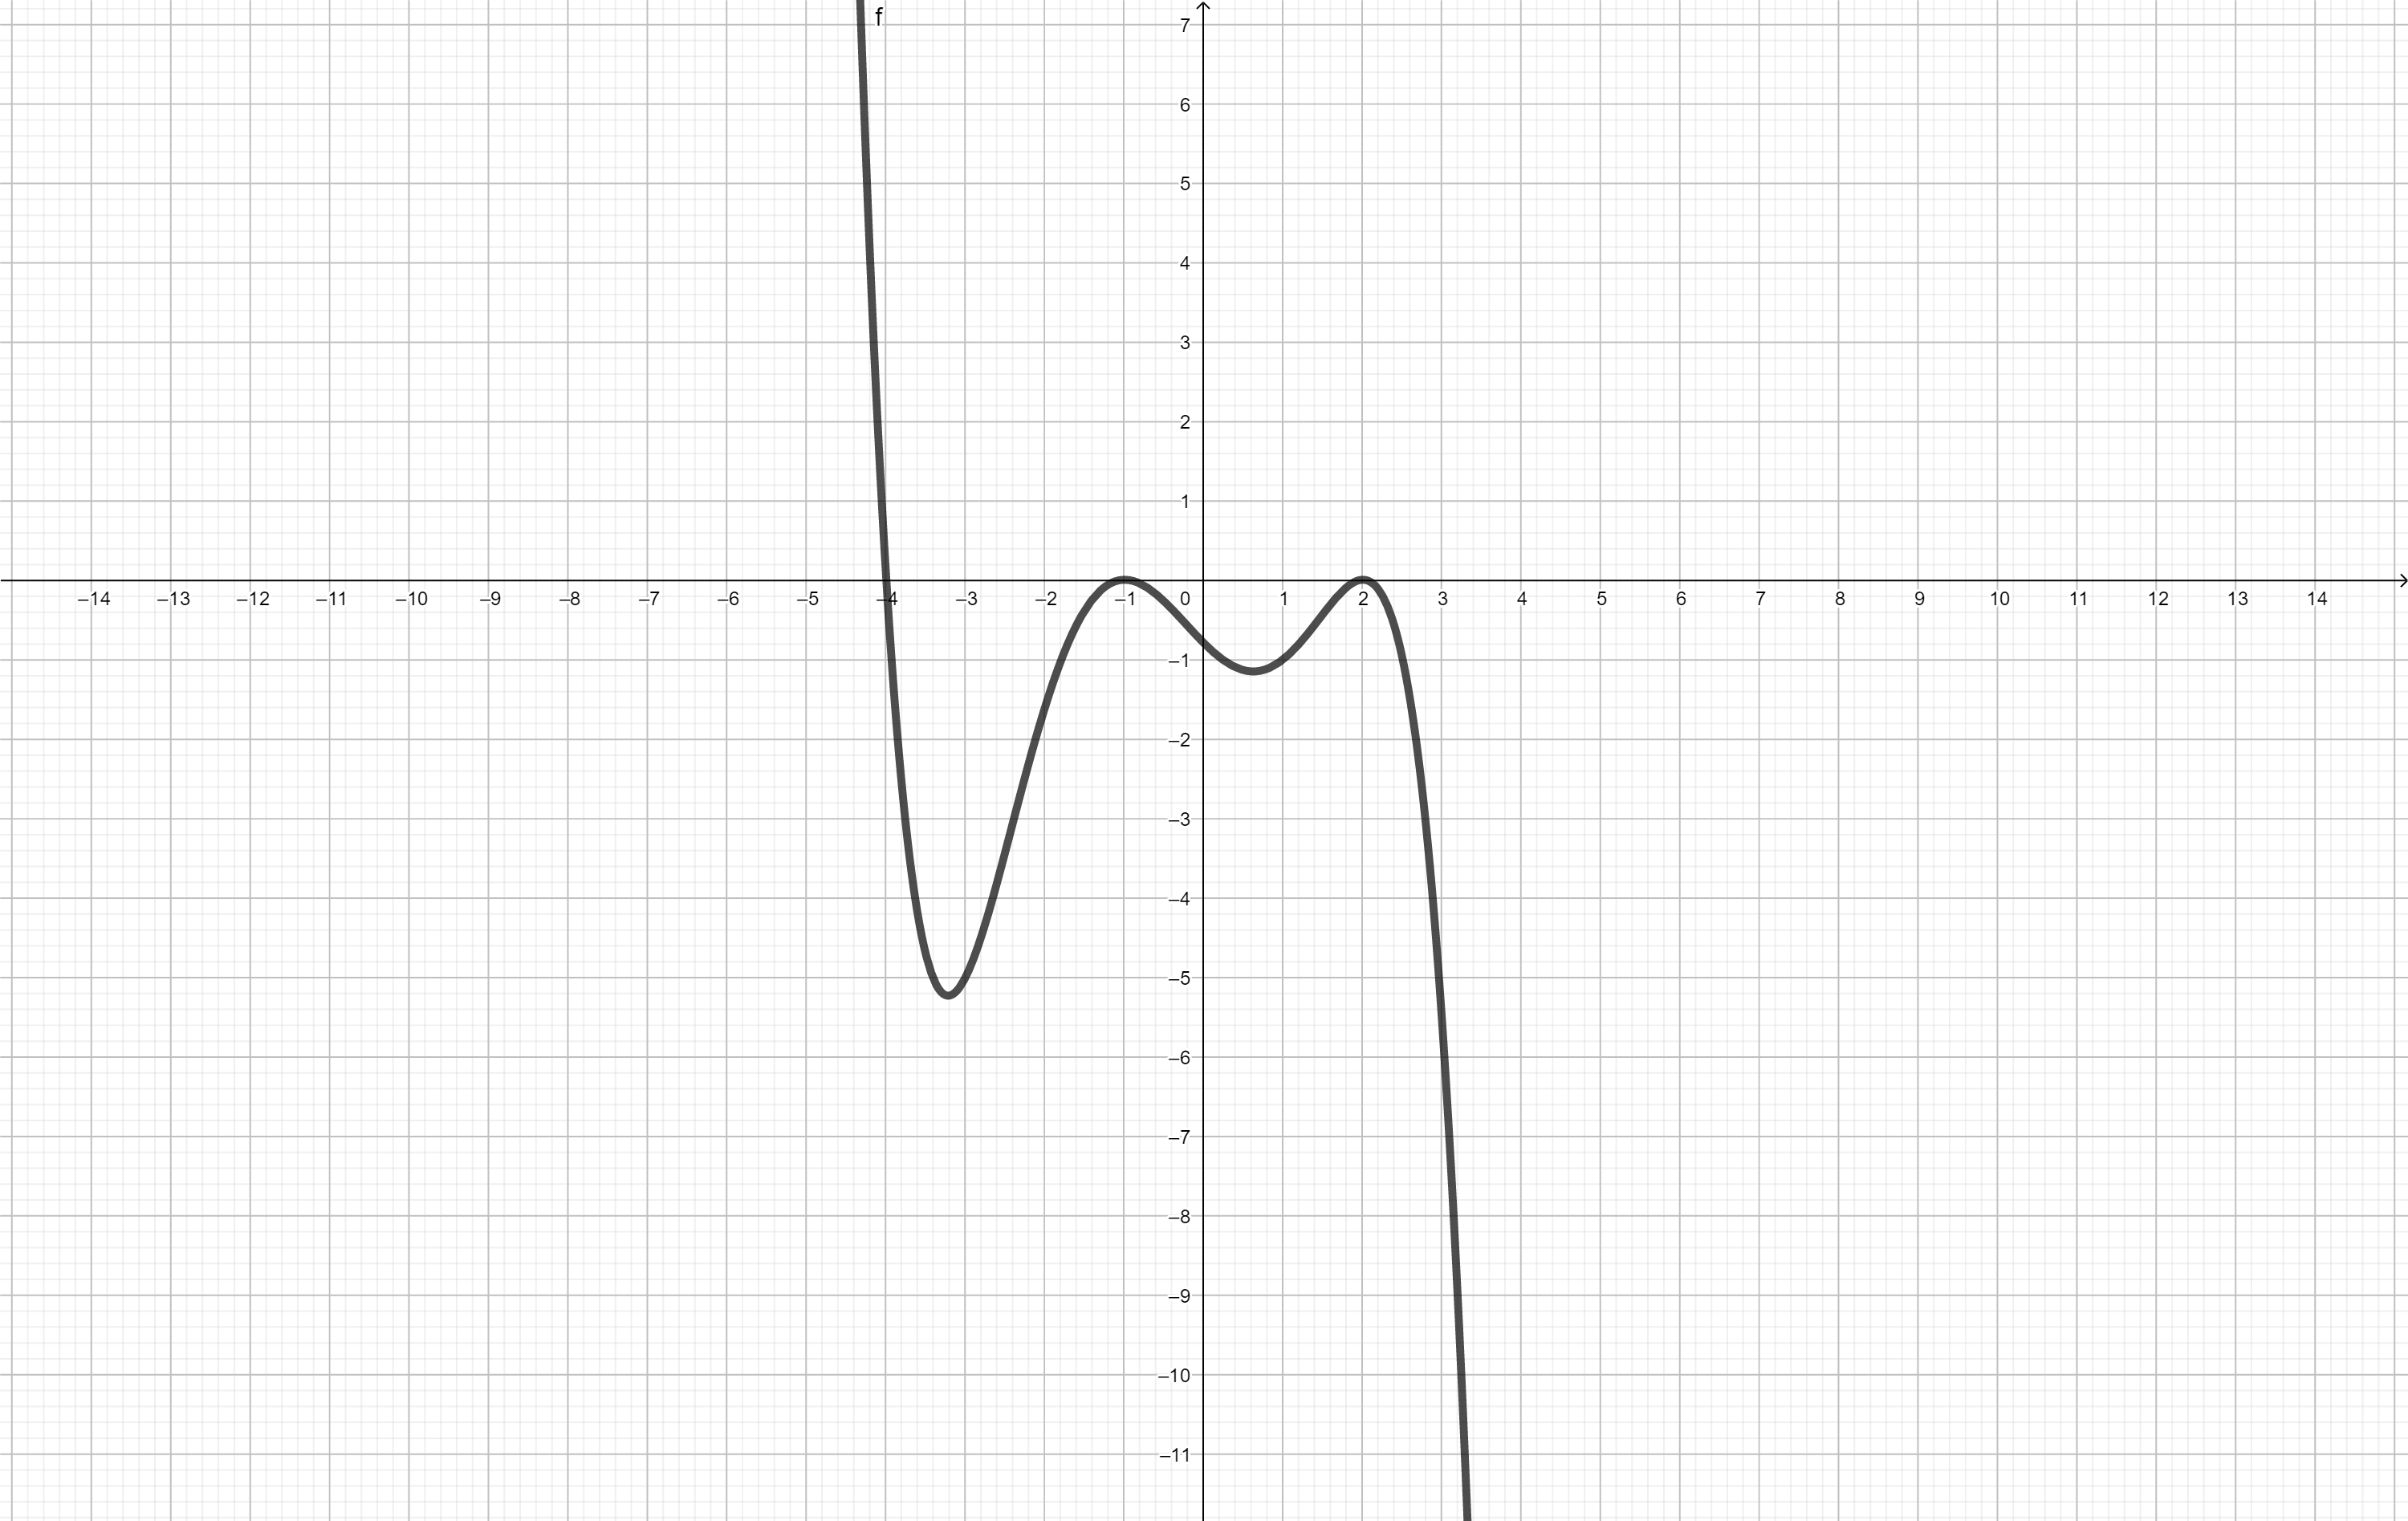
\includegraphics[width=4cm]{Bilder/G511}\hfill
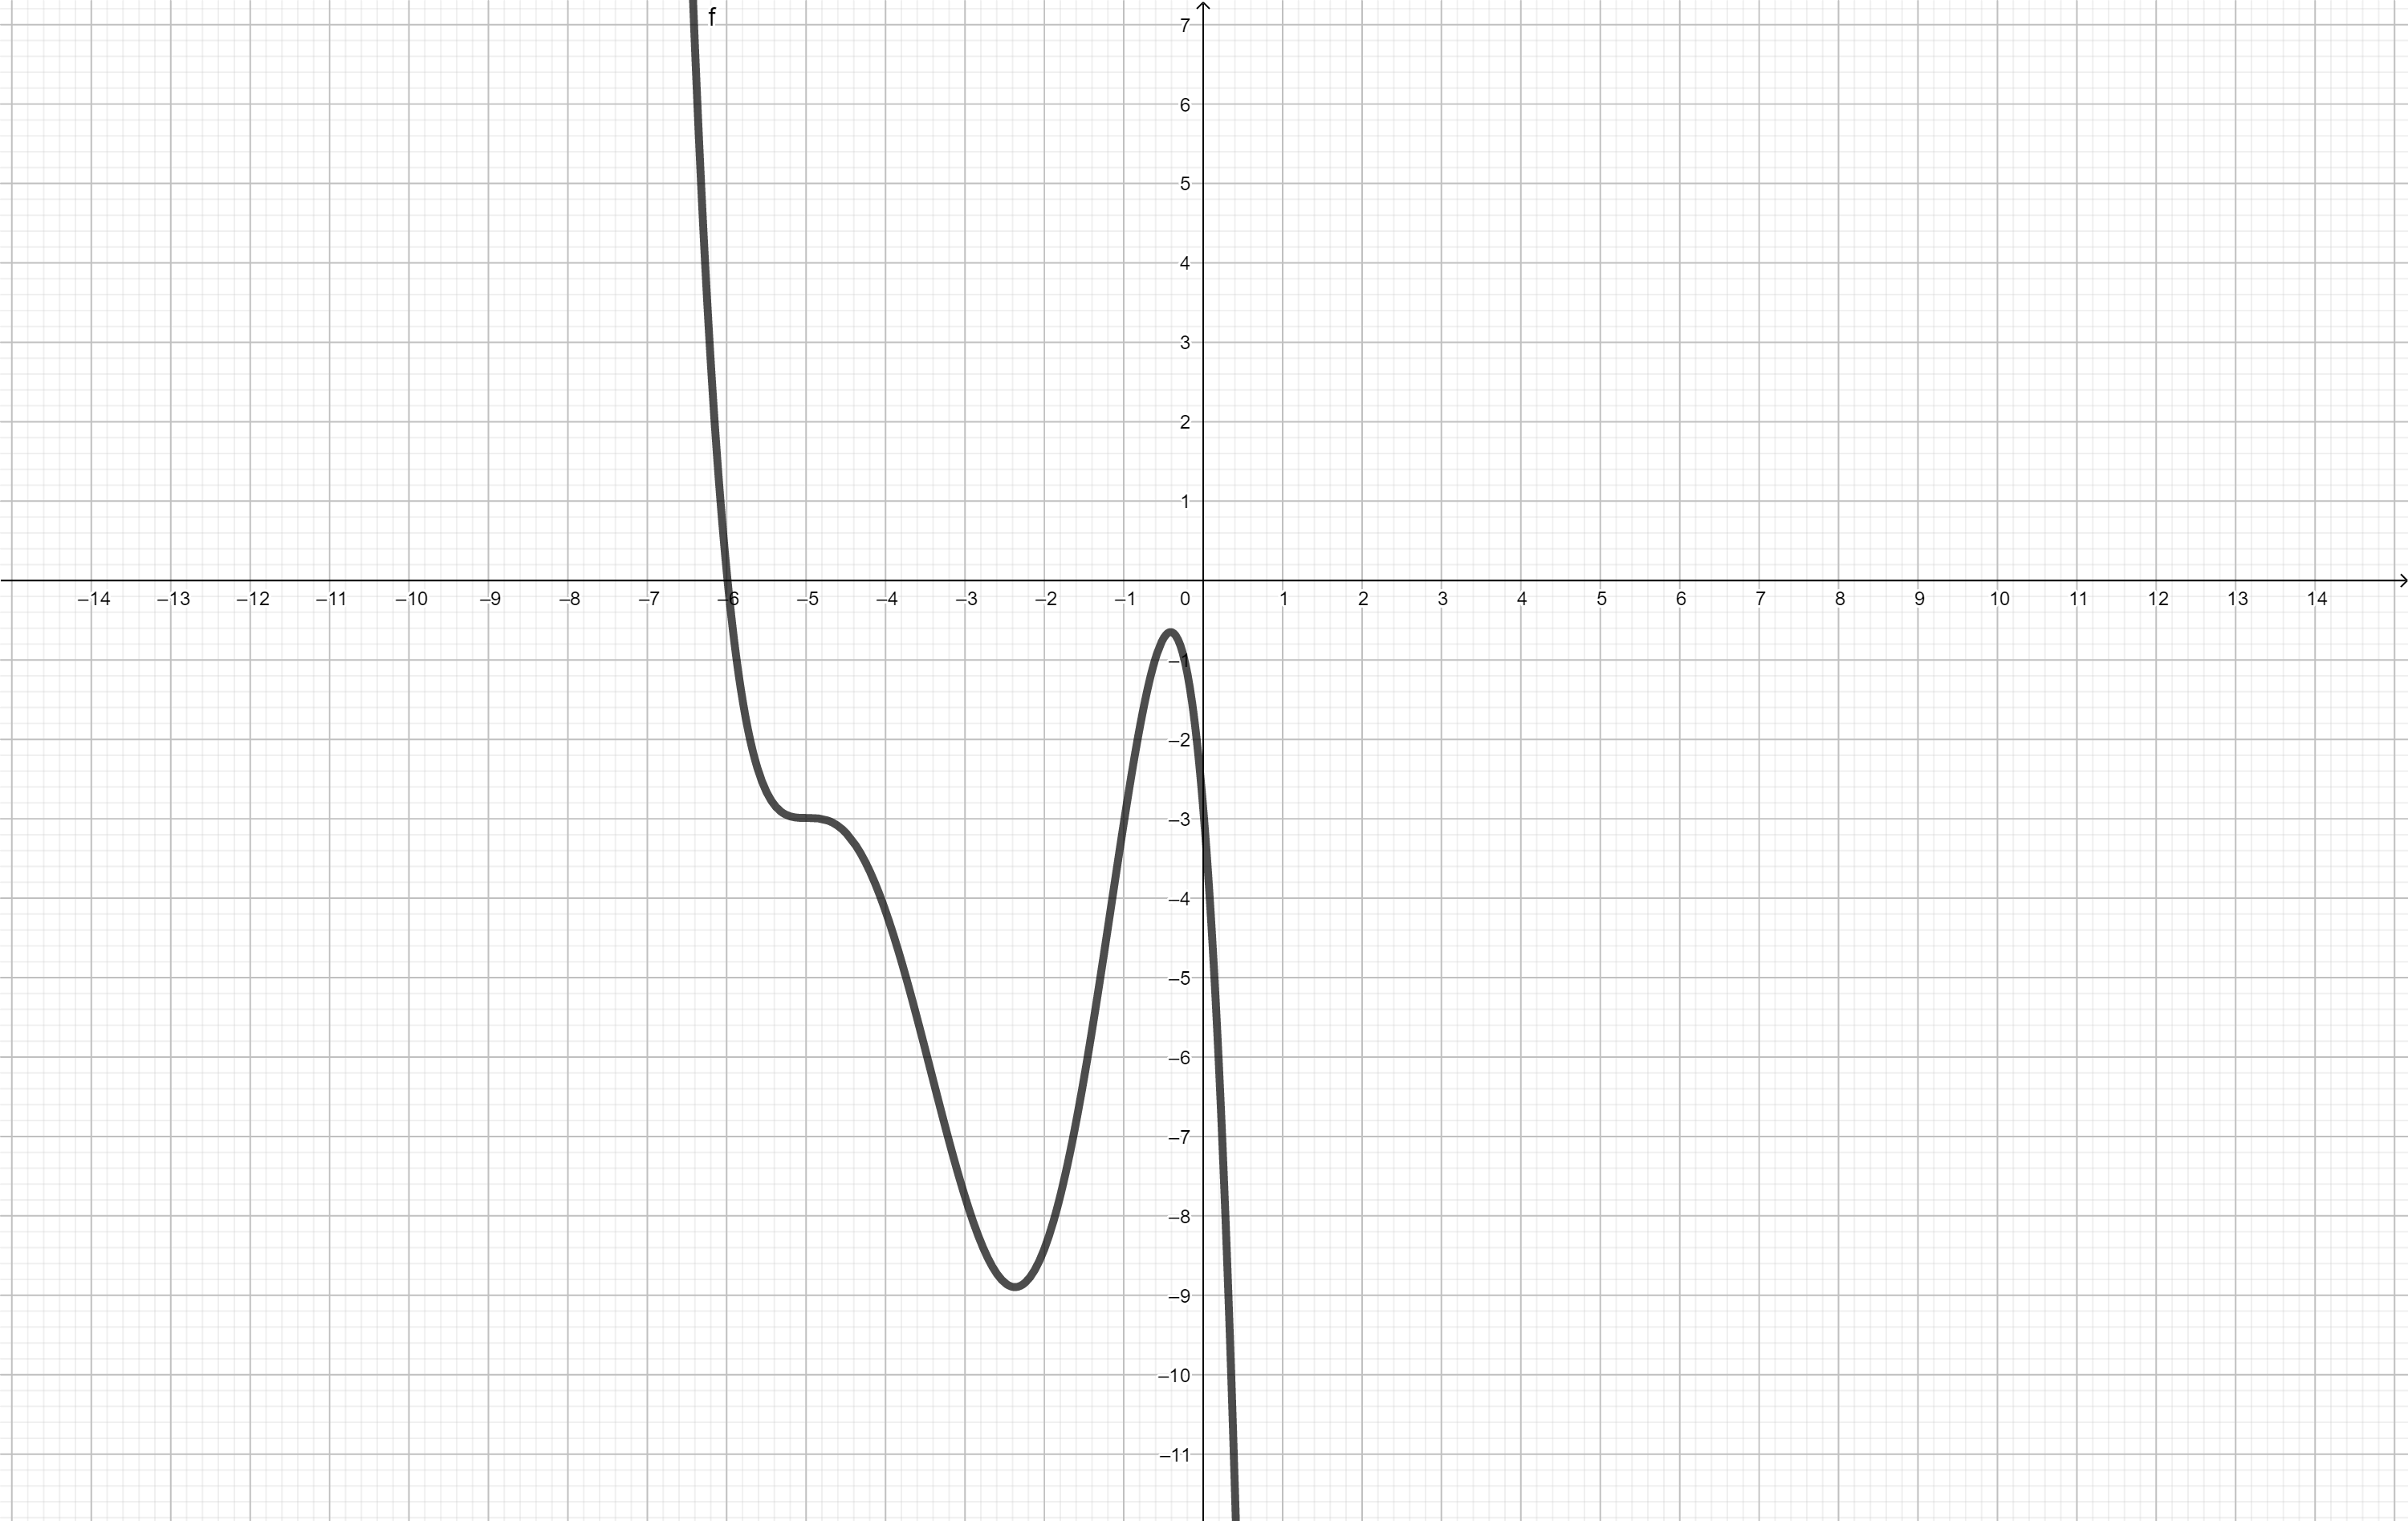
\includegraphics[width=4cm]{Bilder/G512}

\begin{addmargin}[-2cm]{0pt}
Nullstellen:

$x\rightarrow\infty:$

$x\rightarrow-\infty:$
\end{addmargin}

\newpage 

\section*{Ganzrationale Funktionen}
Notiere für jede Funktion die Anzahl der Hoch-/Tief- und Wendepunkte! Notiere außerdem die Summe der Hoch- und Tiefunkte!

\paragraph{Grad 1:}\textcolor{white}{.}\\
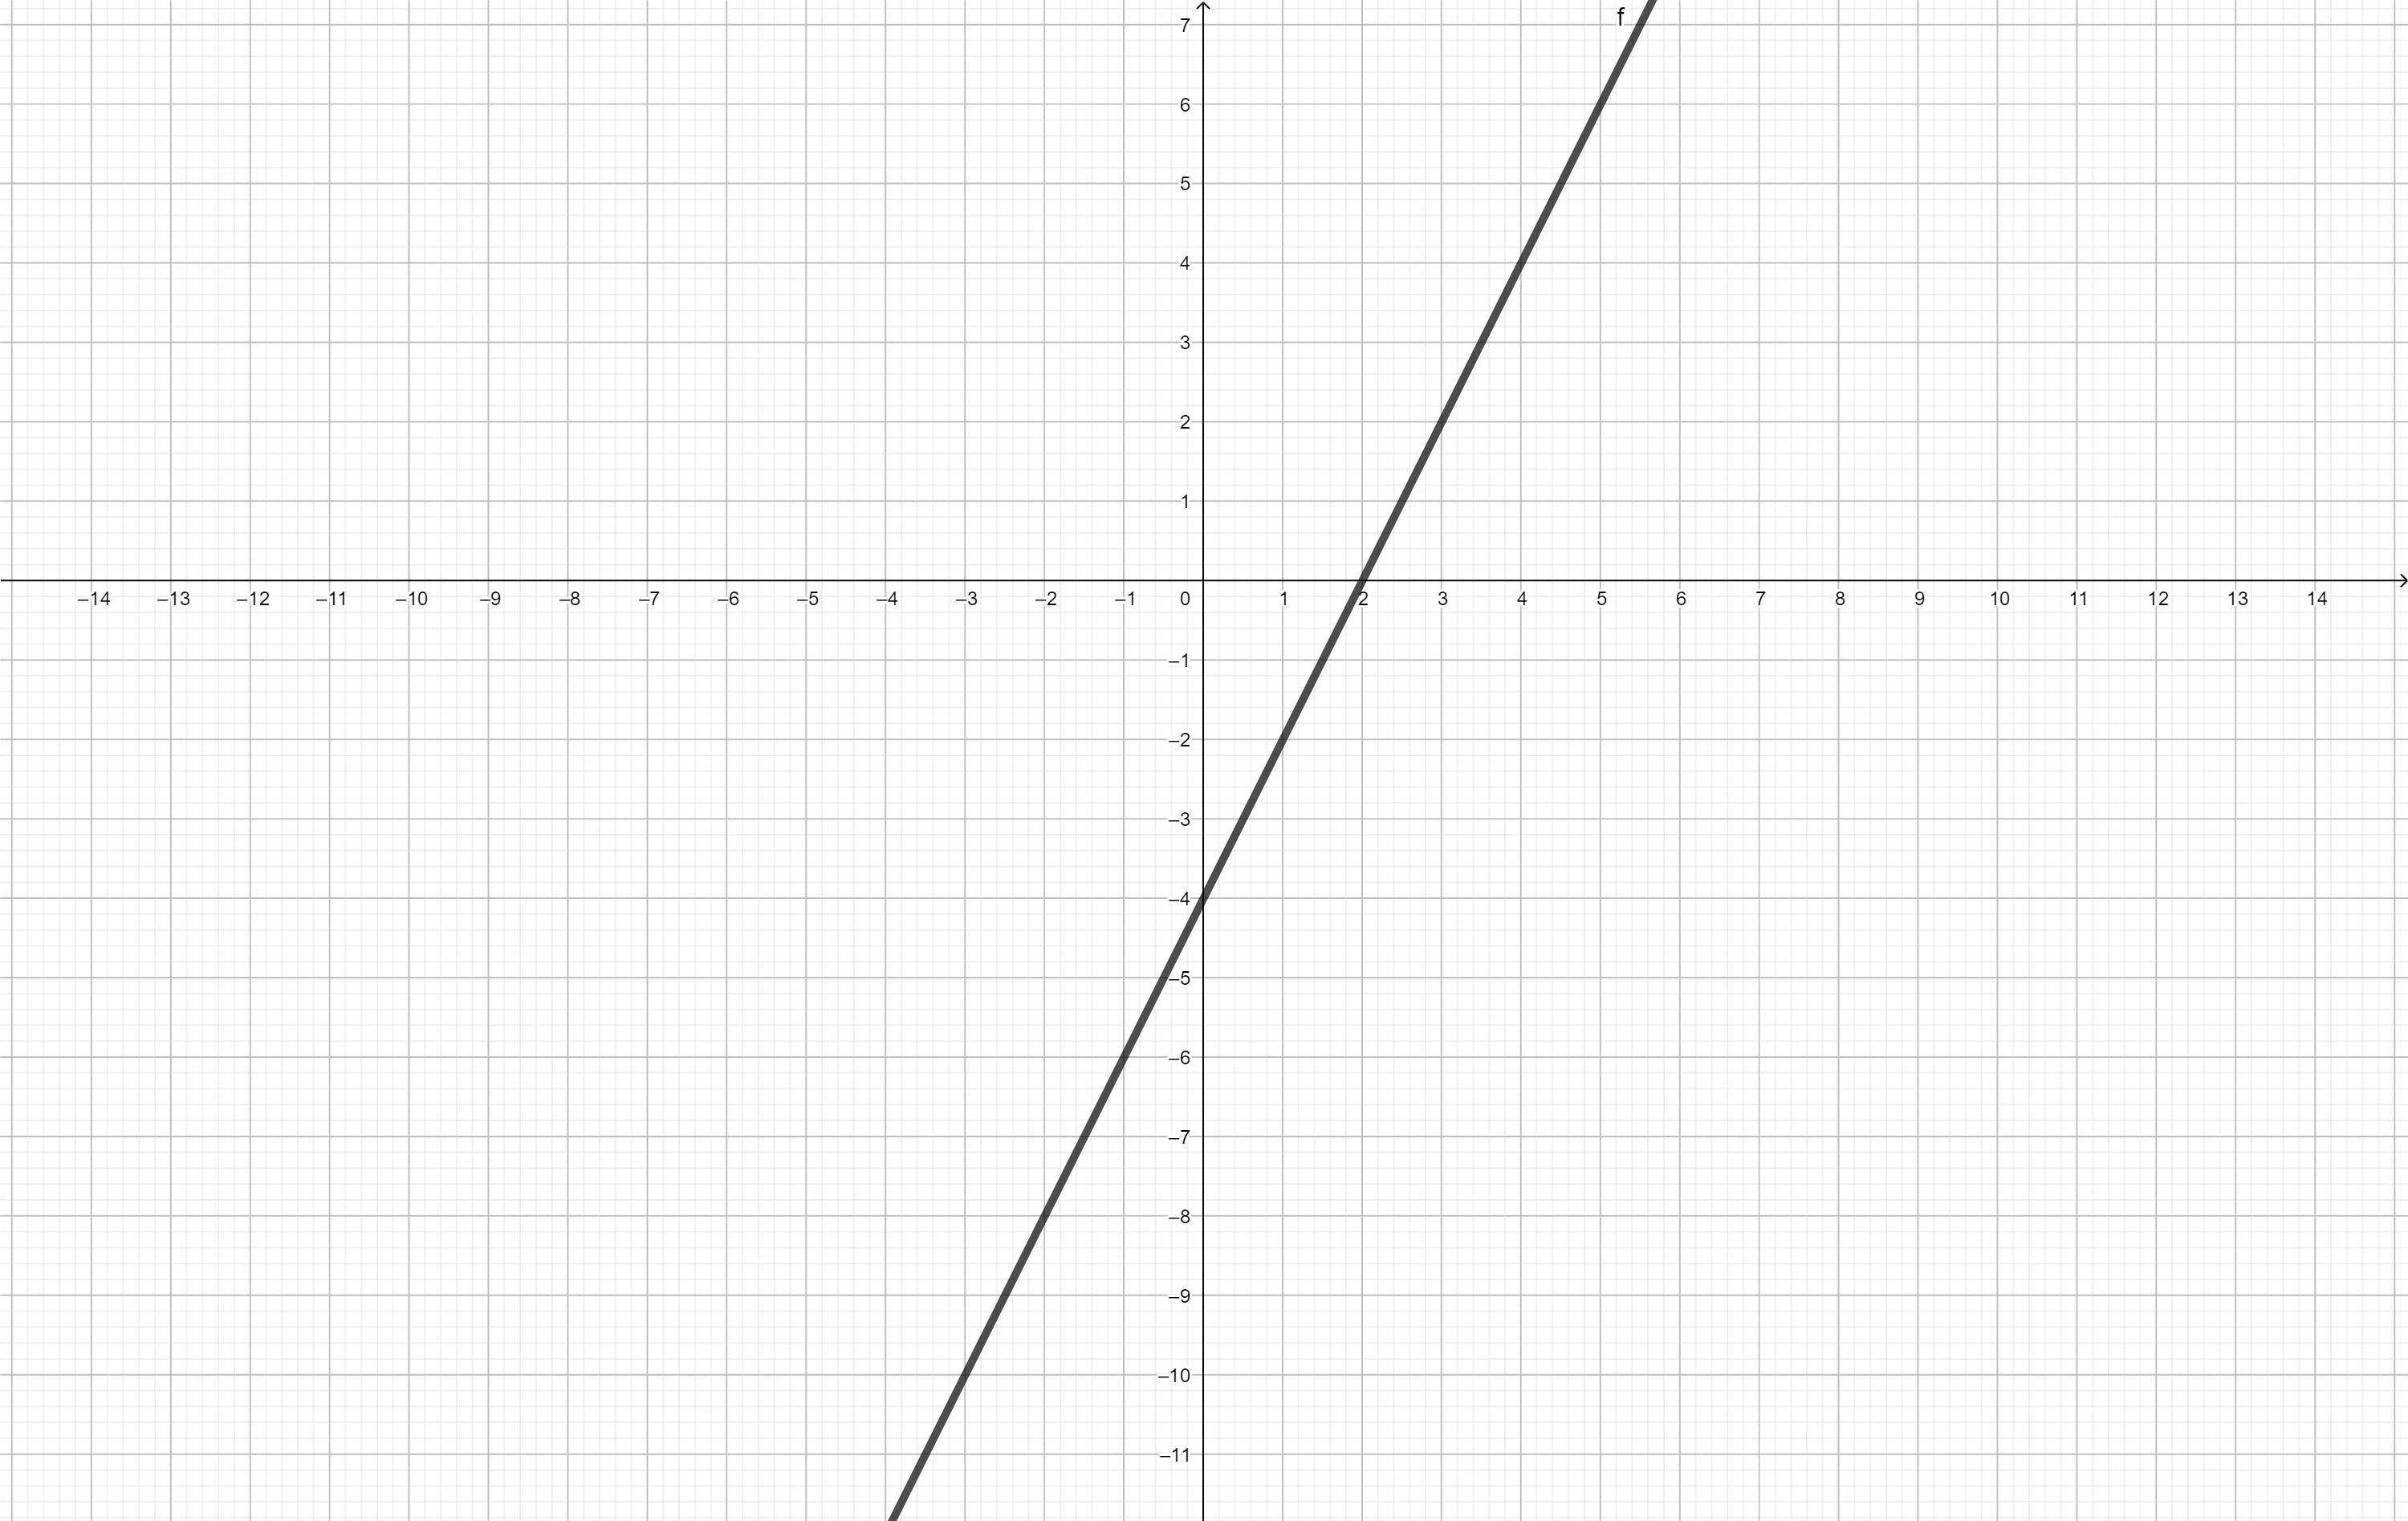
\includegraphics[width=4cm]{Bilder/G11}\hfill
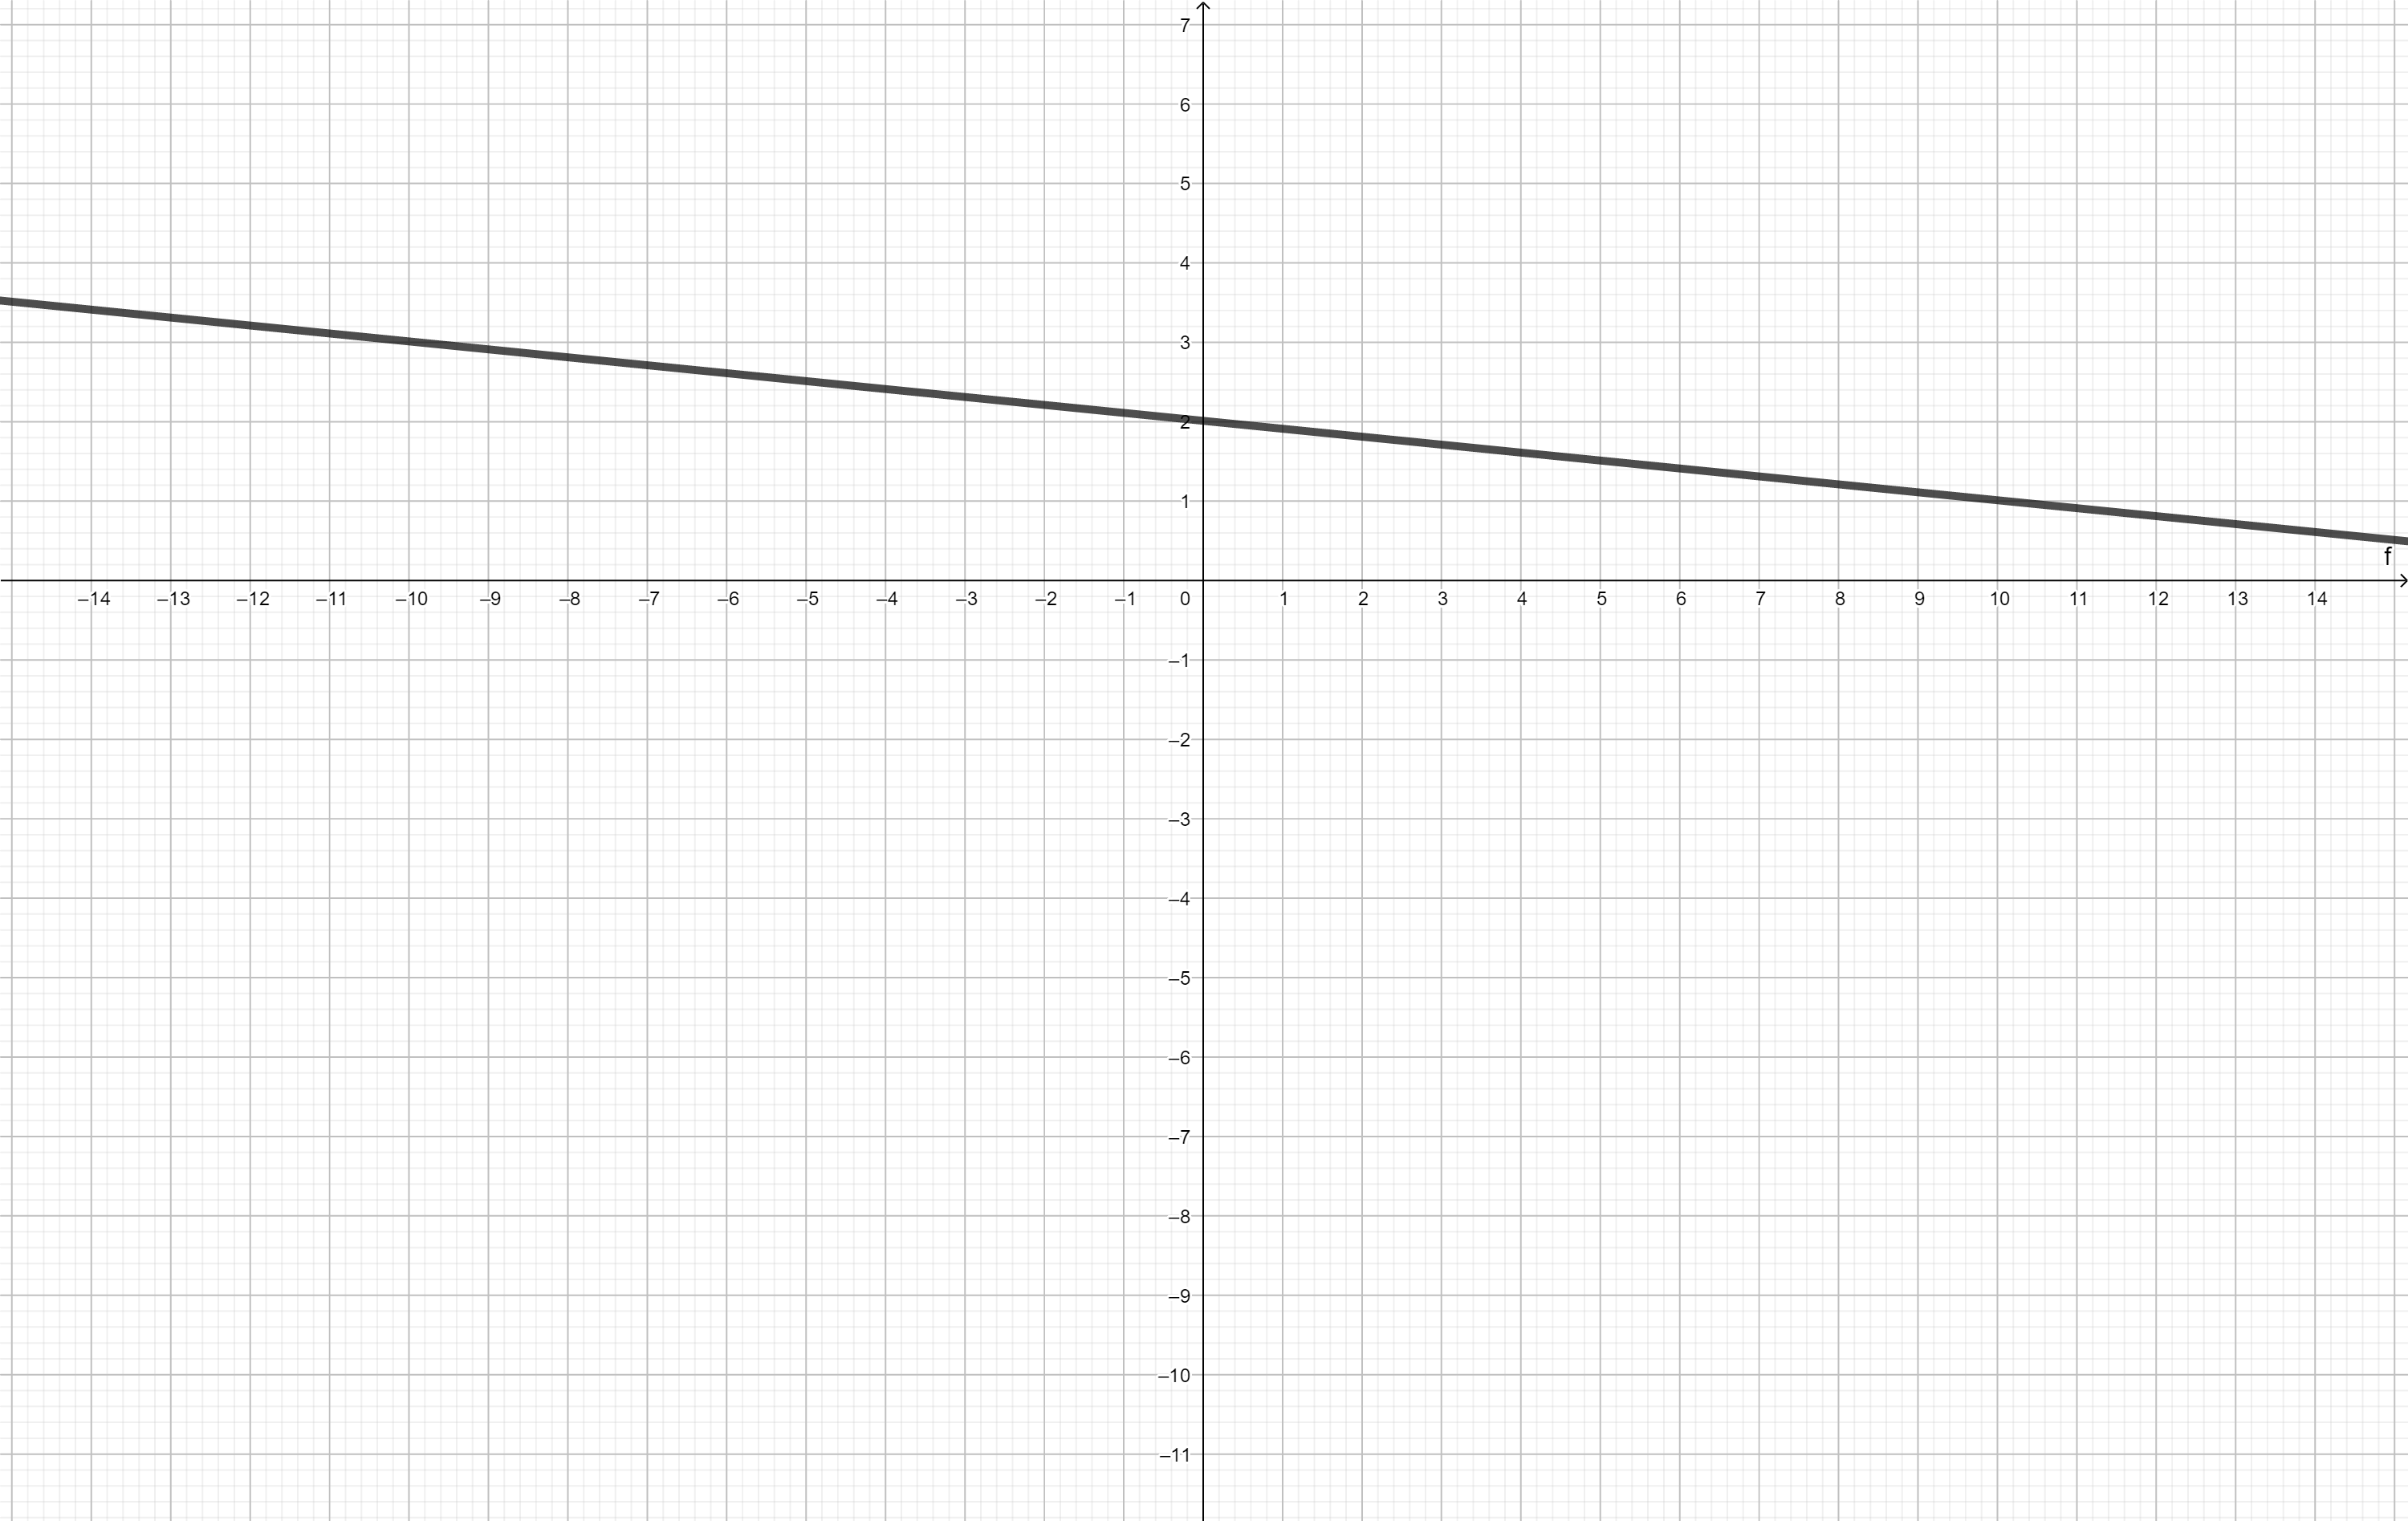
\includegraphics[width=4cm]{Bilder/G12}\hfill
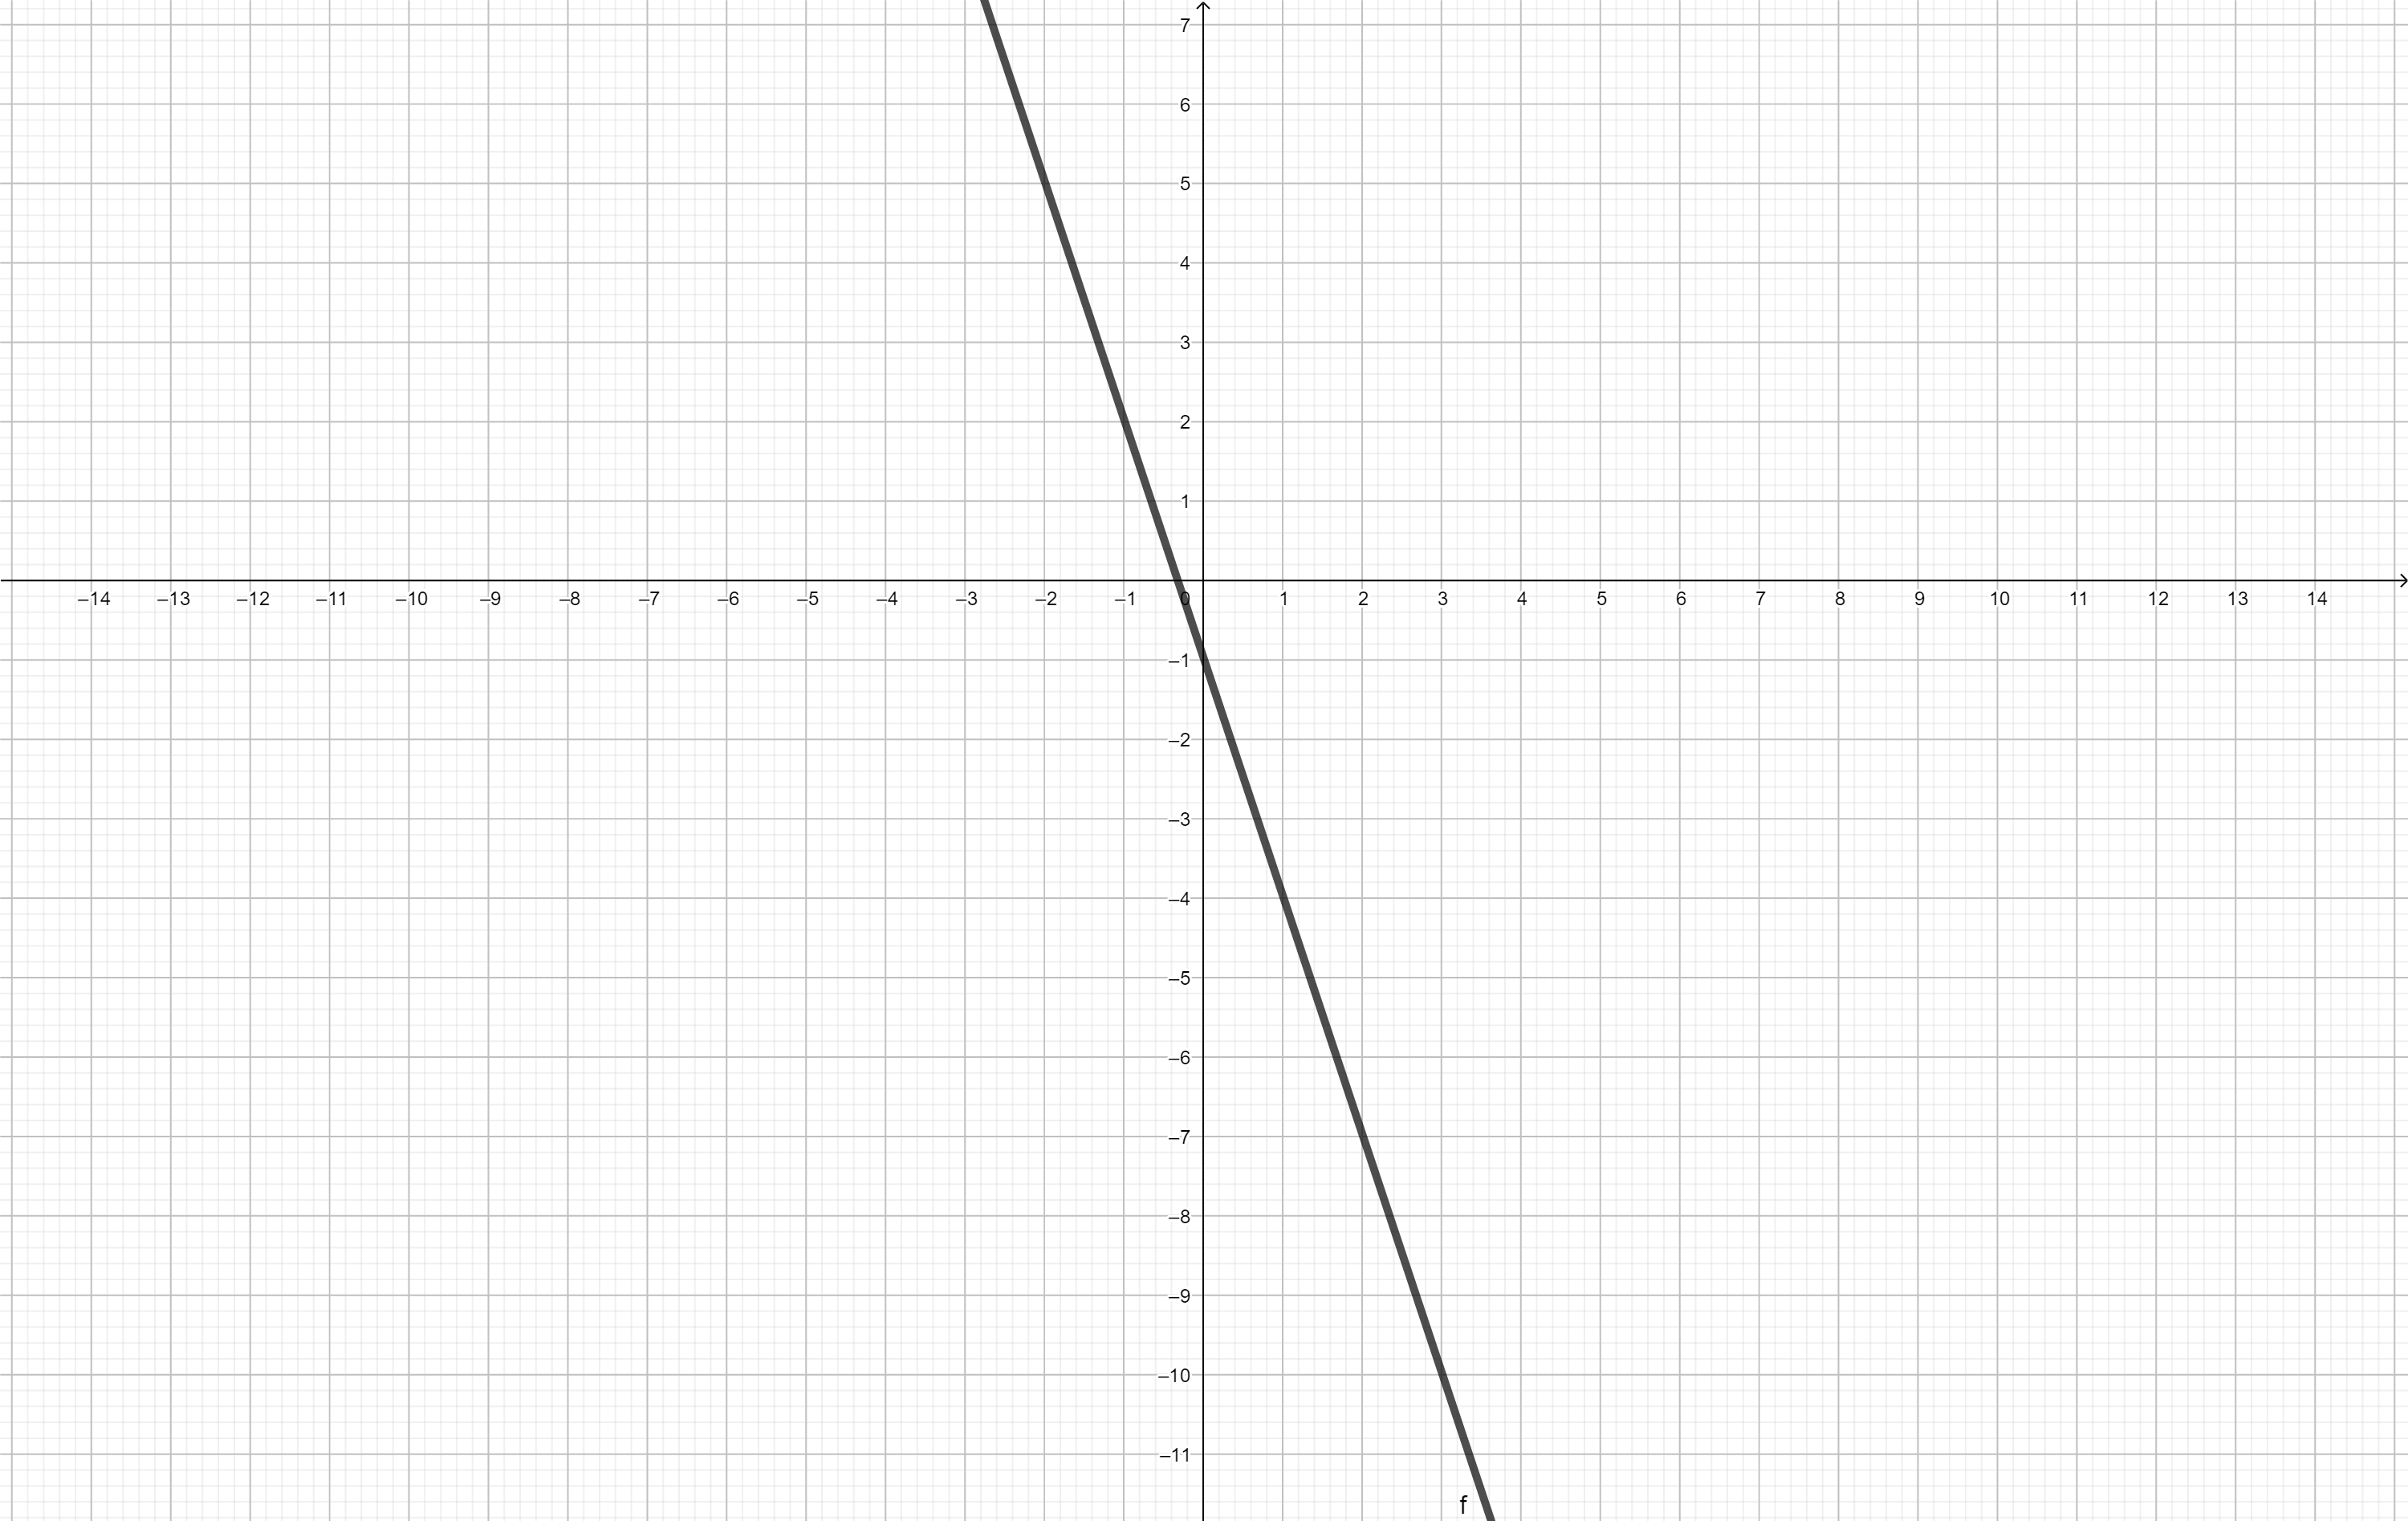
\includegraphics[width=4cm]{Bilder/G13}\hfill
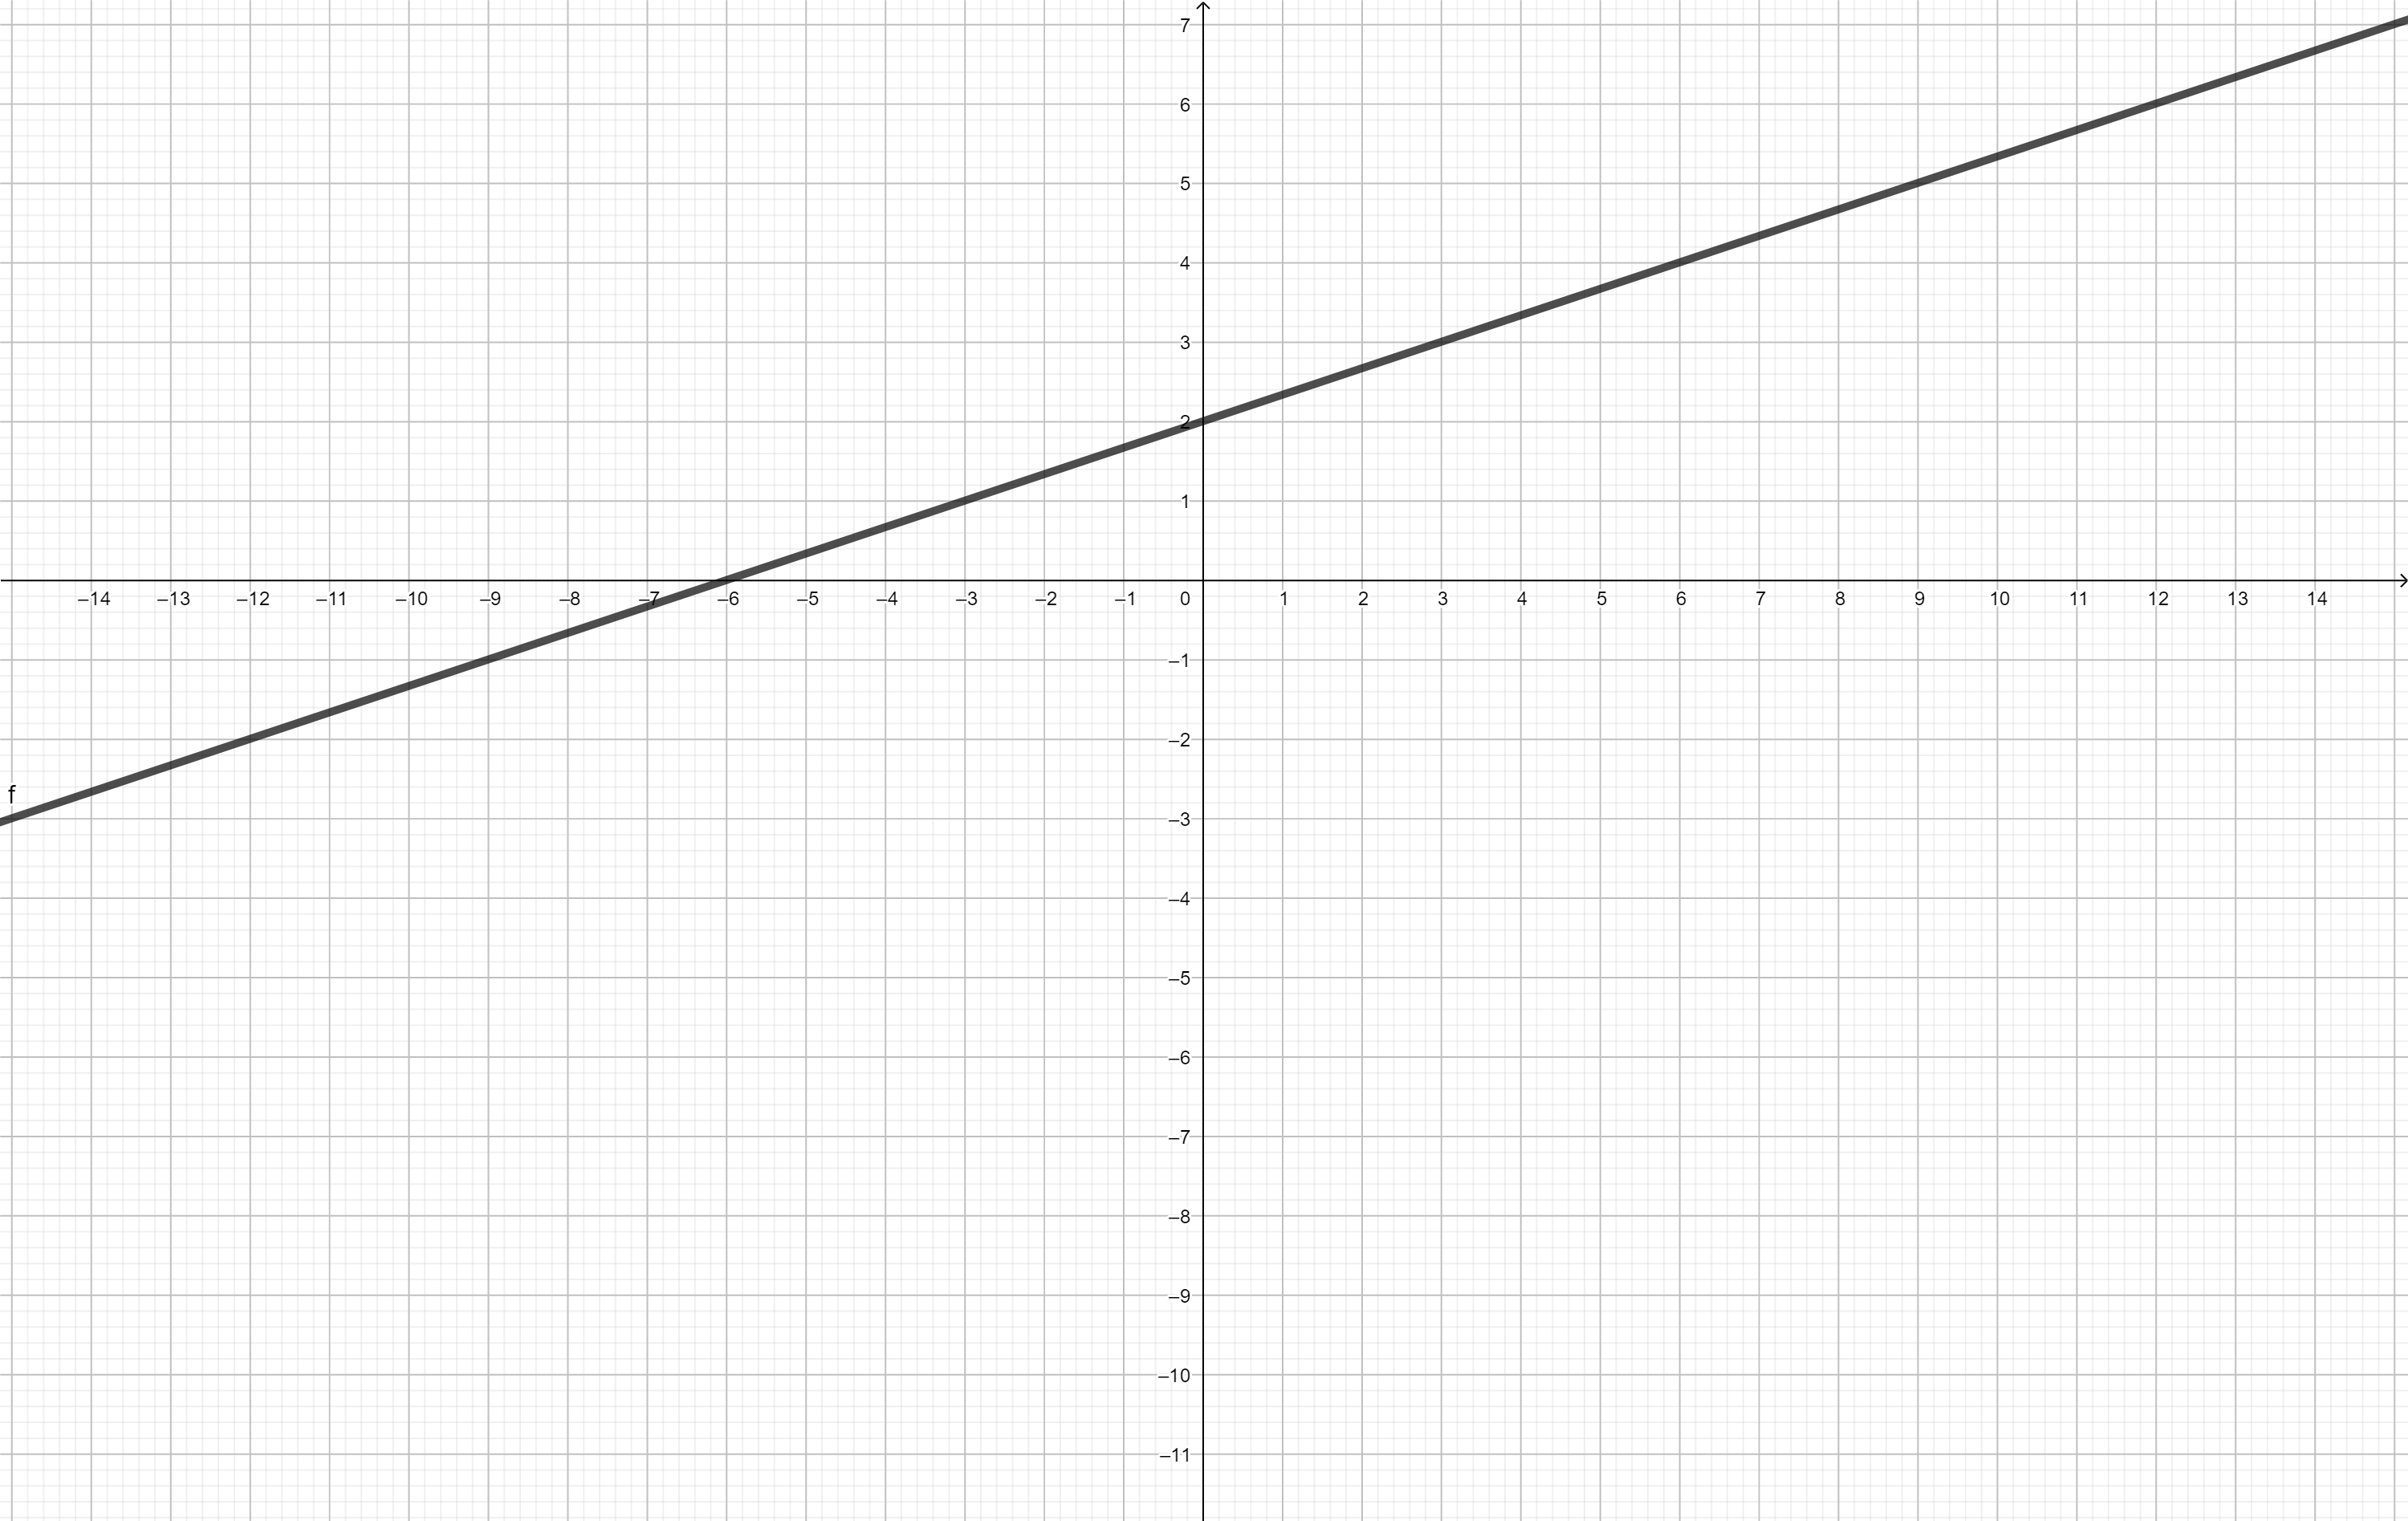
\includegraphics[width=4cm]{Bilder/G14}

\begin{addmargin}[-2cm]{0pt}
Hochpunkte: \\
Tiefpunkte: \\
Summe: \\
Wendepunkte:
\end{addmargin}

\paragraph{Grad 2:}\textcolor{white}{.}\\
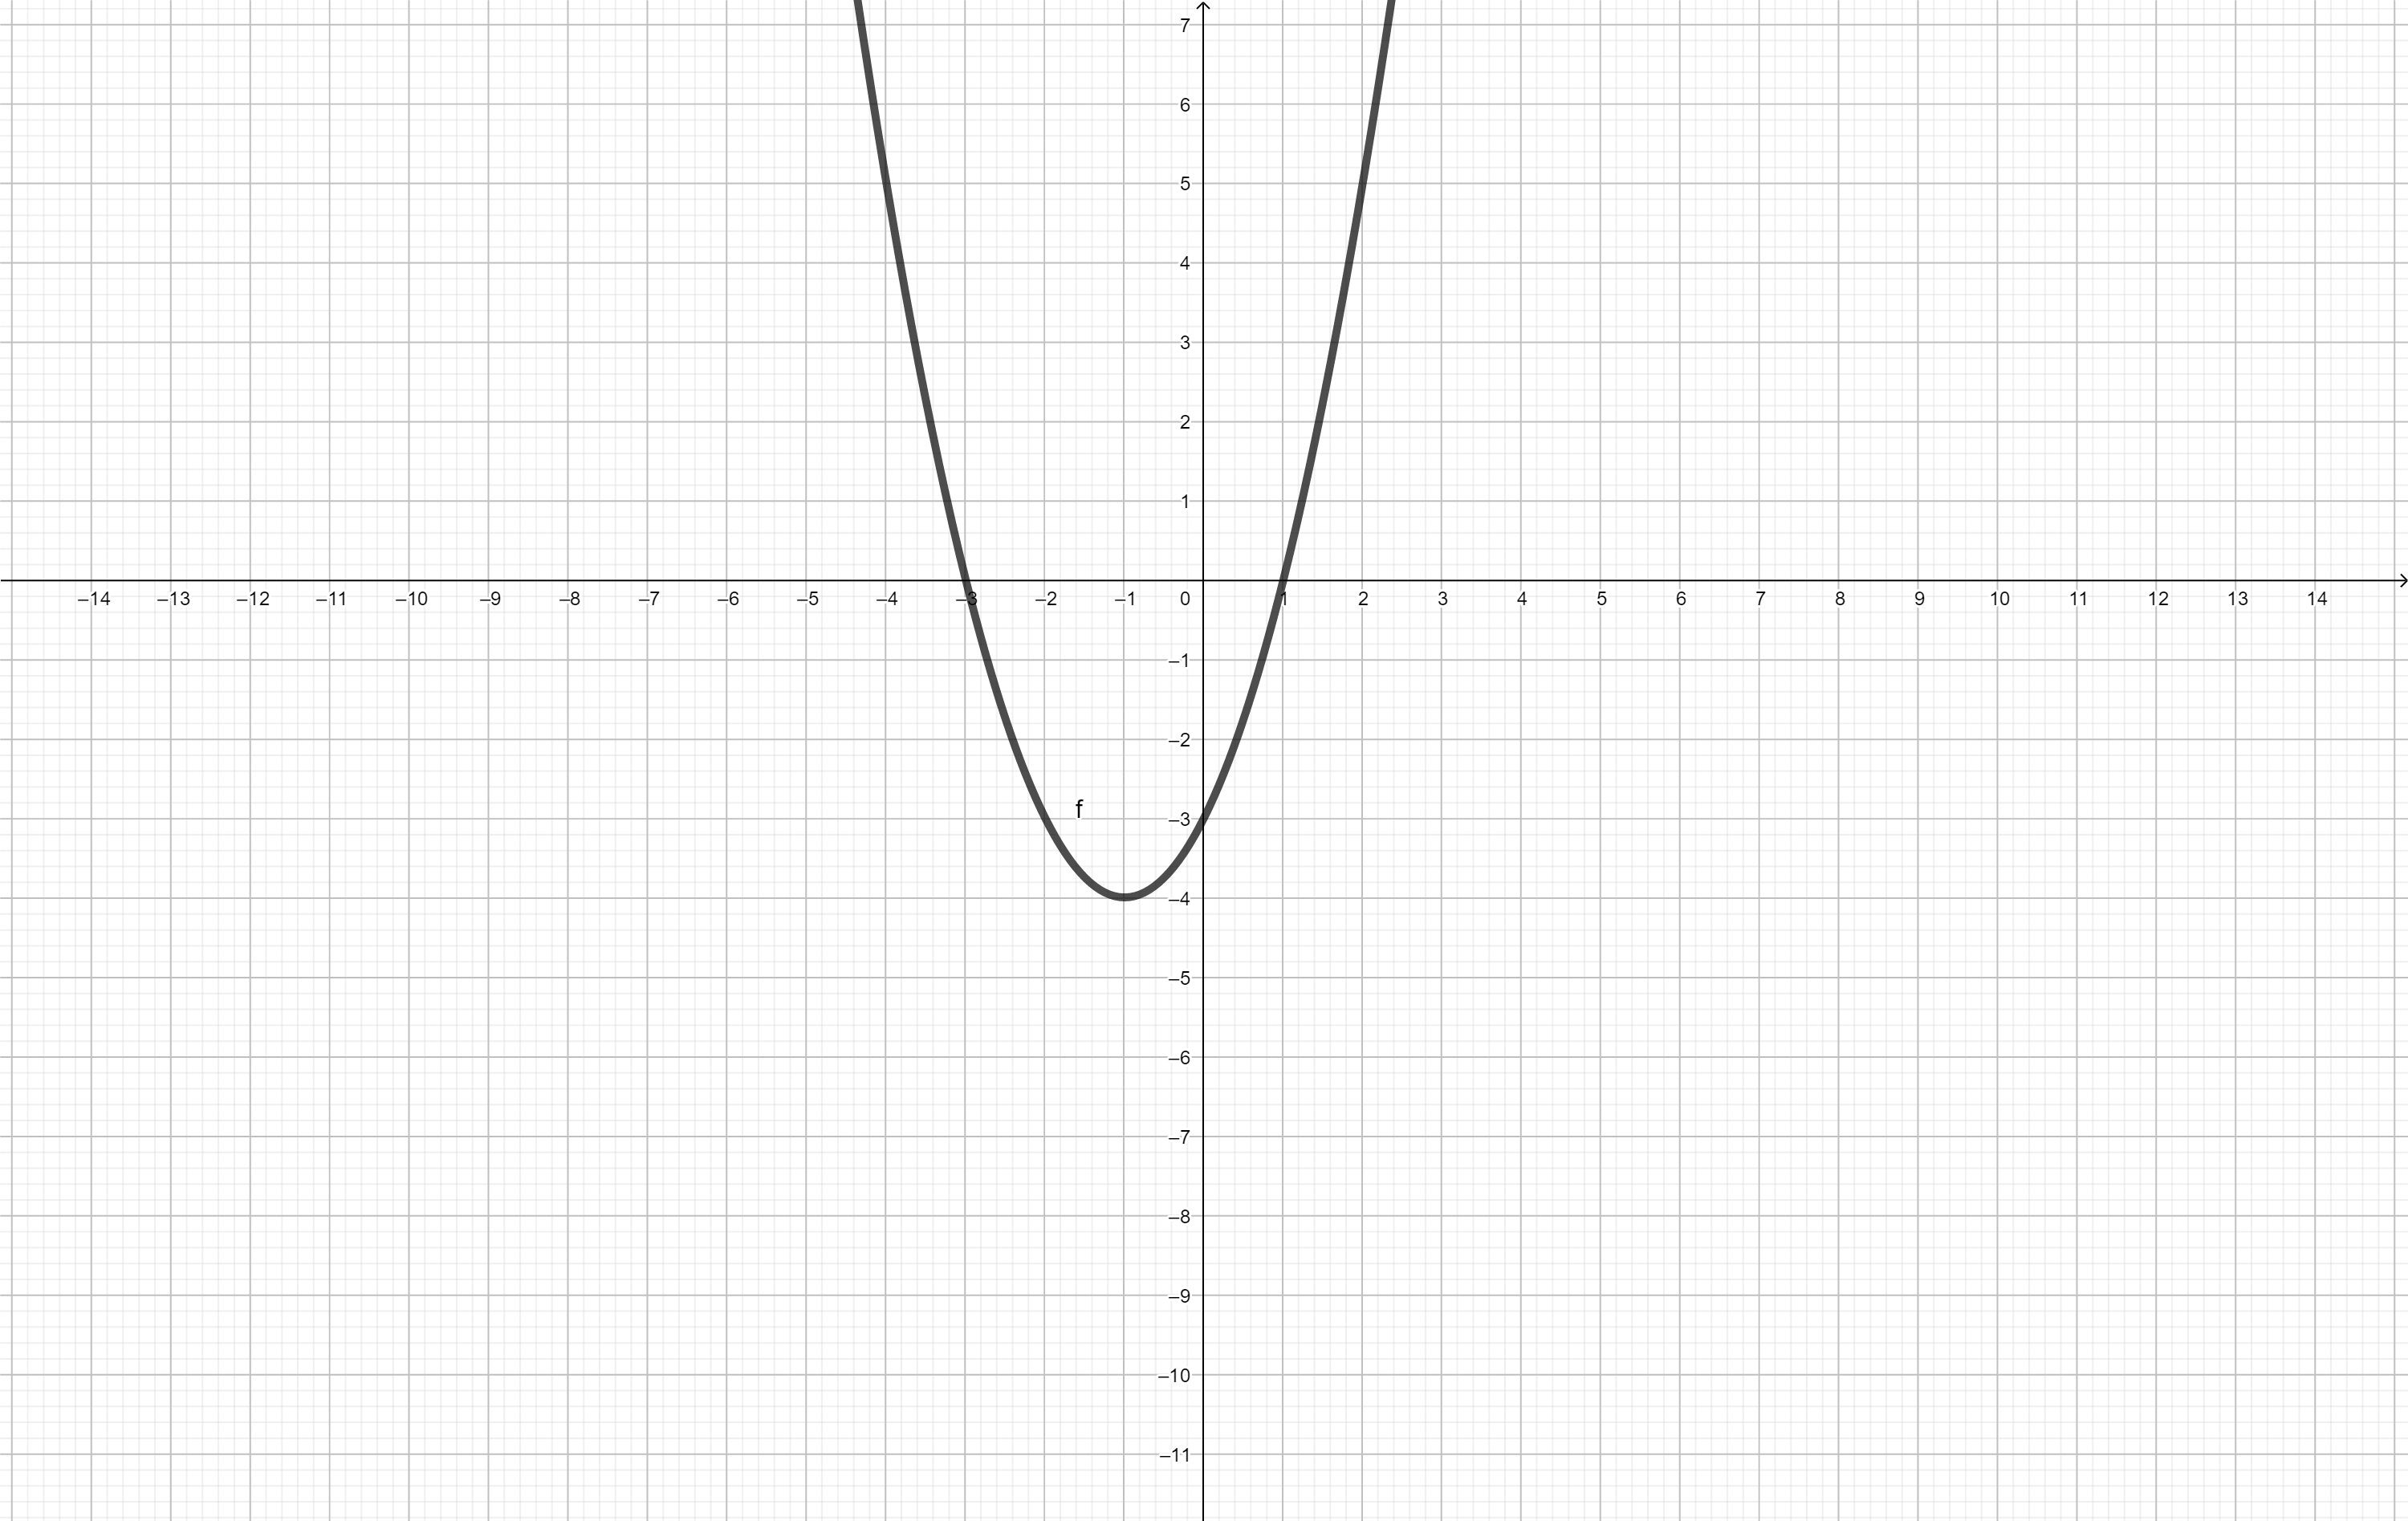
\includegraphics[width=4cm]{Bilder/G21}\hfill
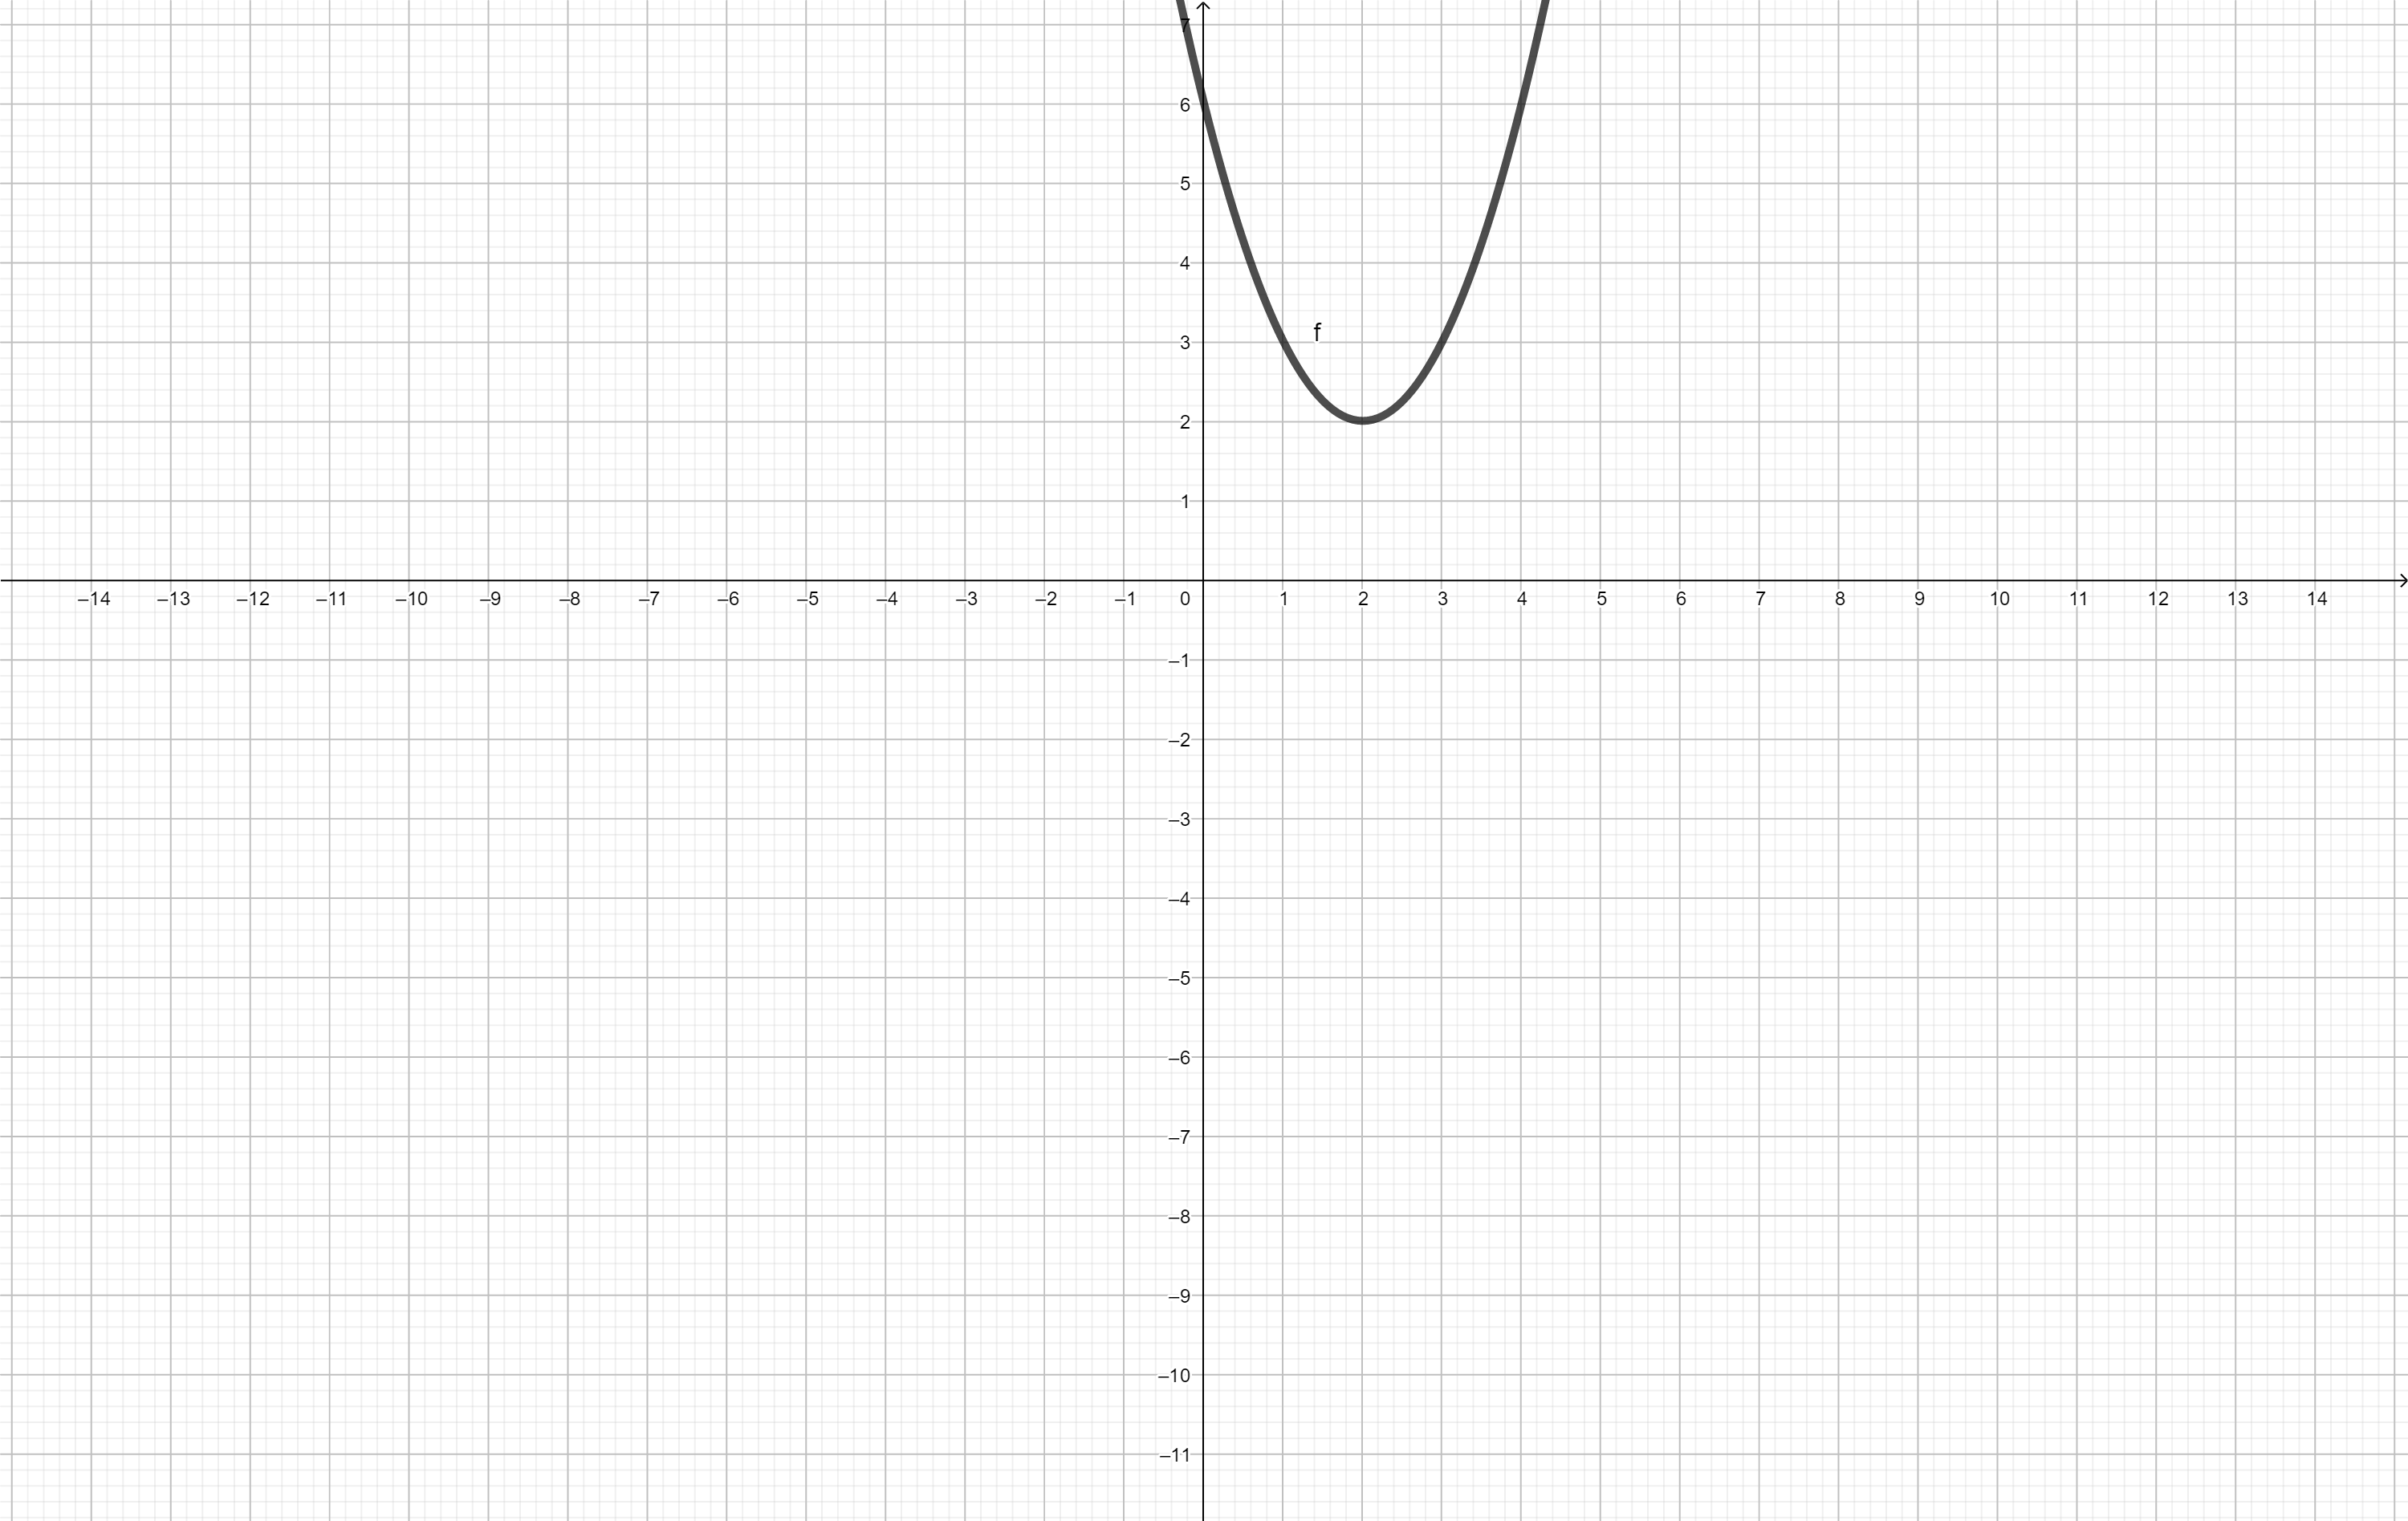
\includegraphics[width=4cm]{Bilder/G22}\hfill
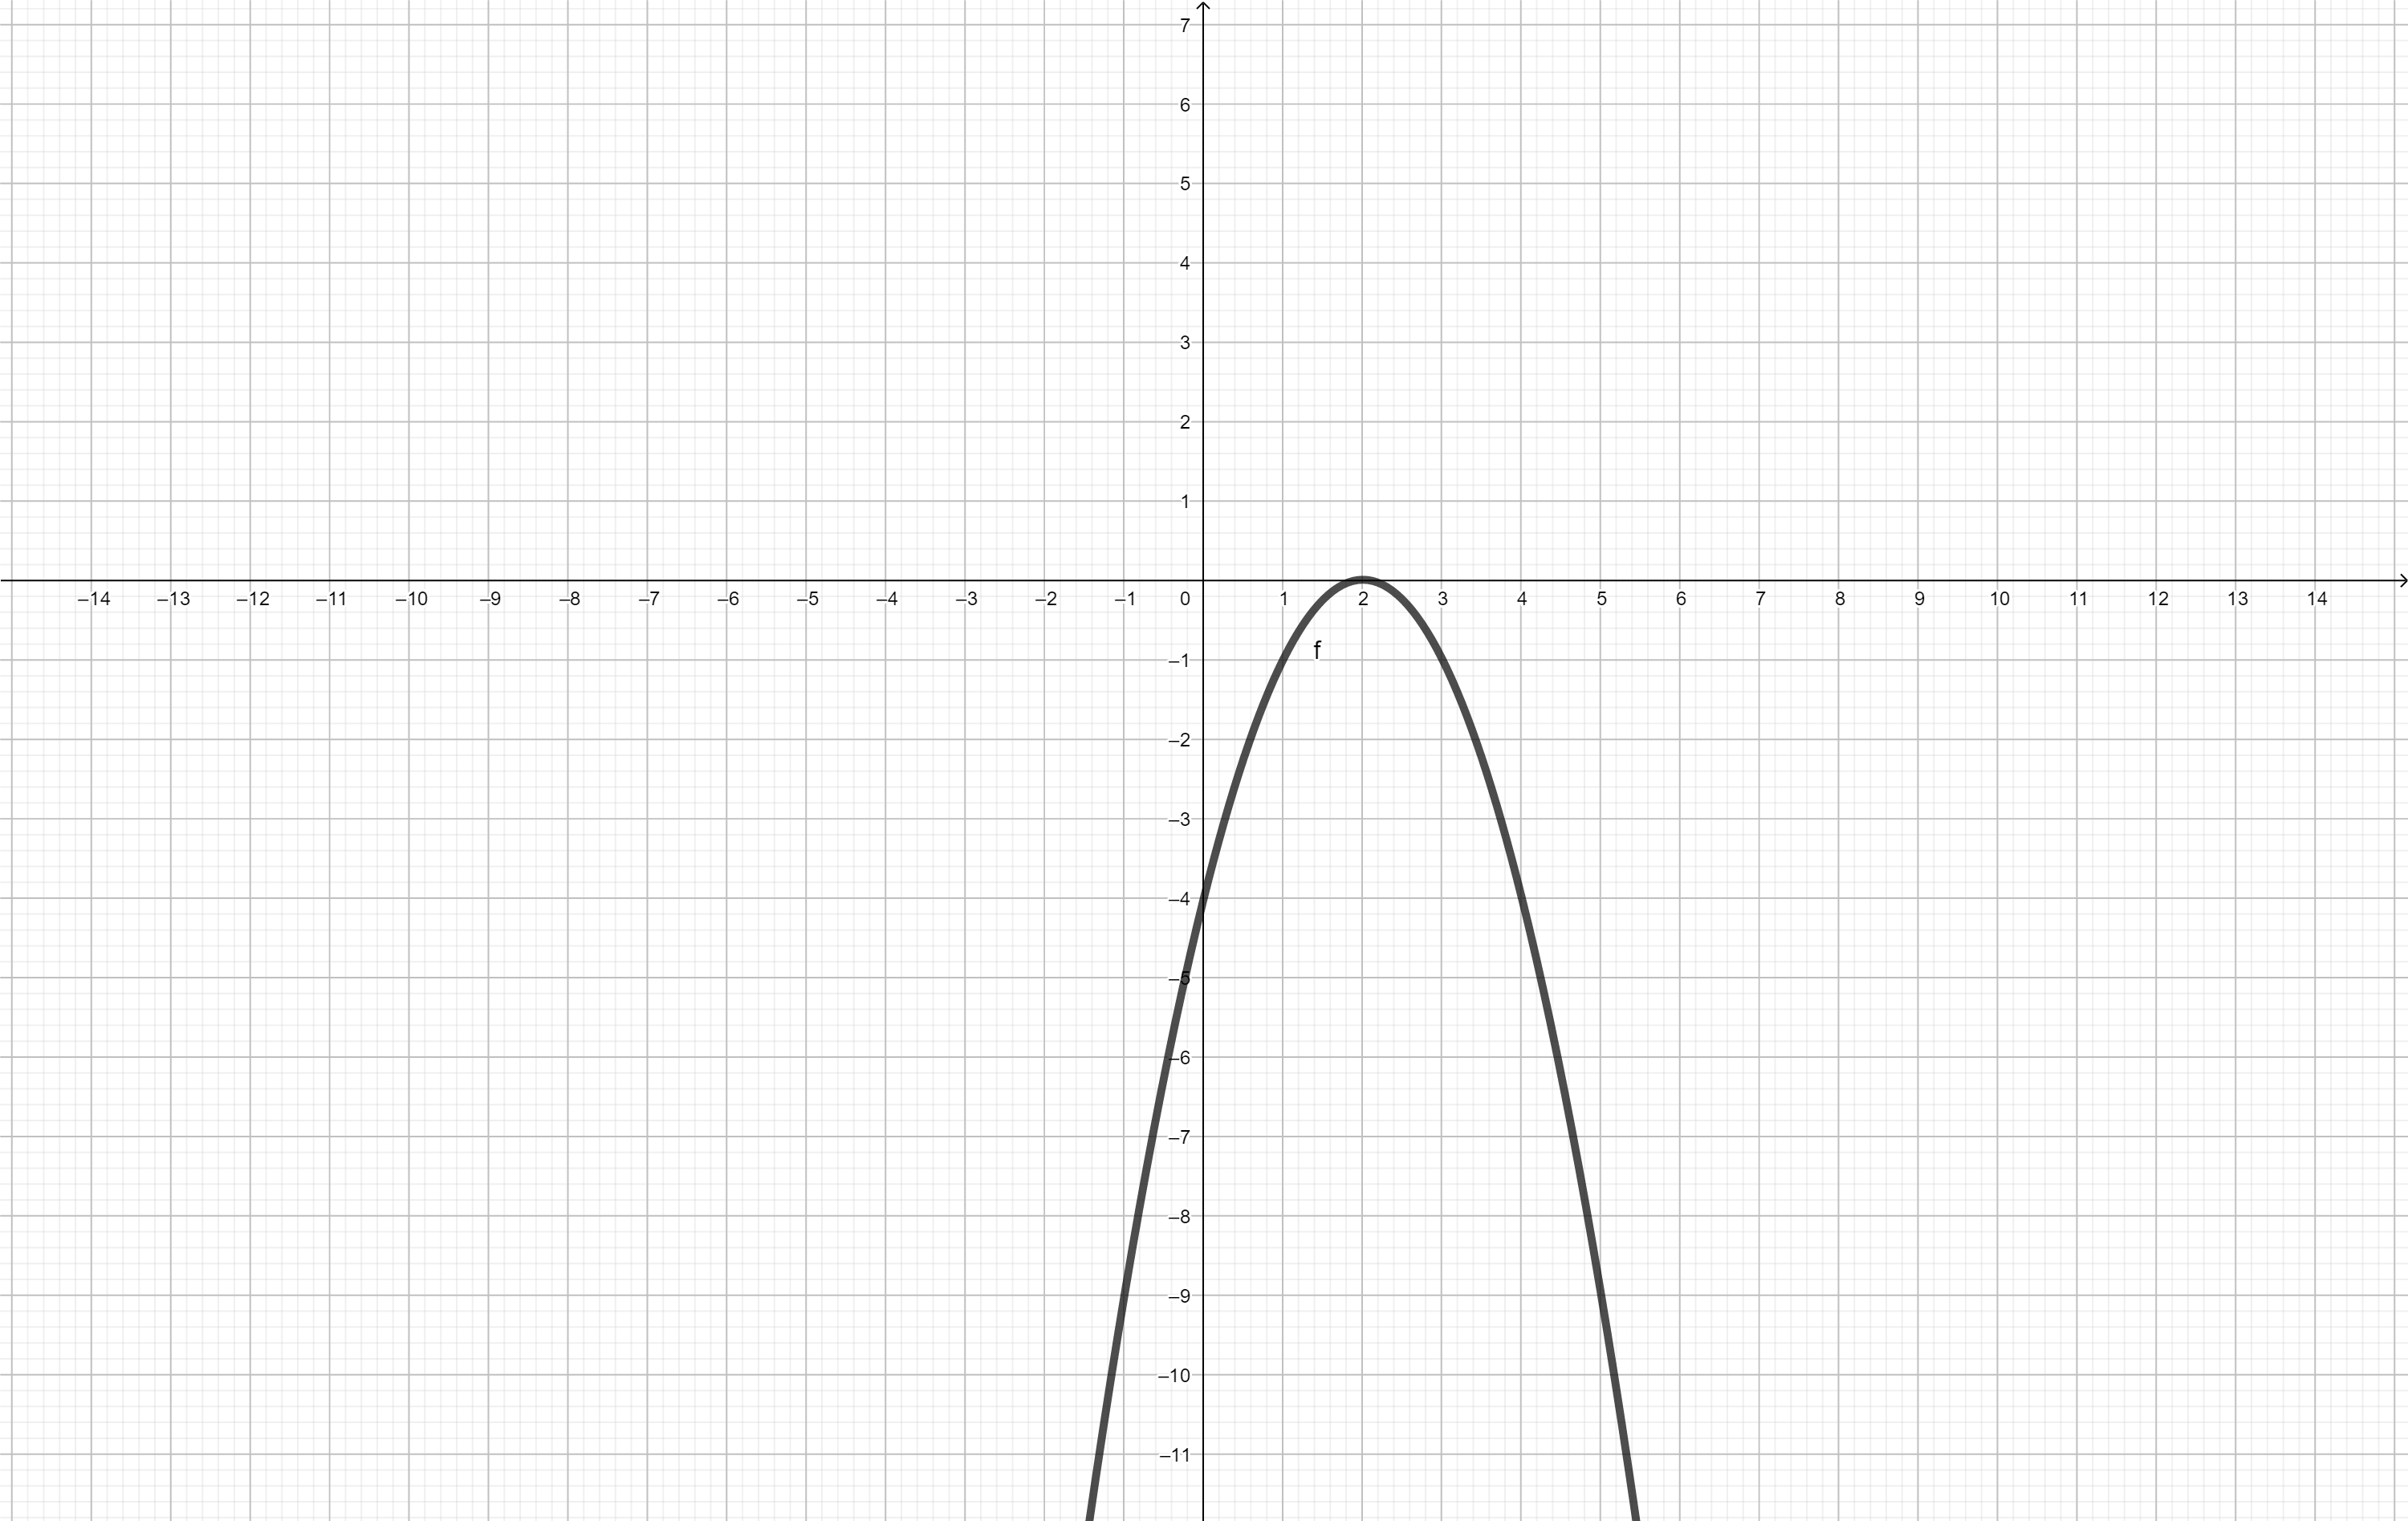
\includegraphics[width=4cm]{Bilder/G23}\hfill
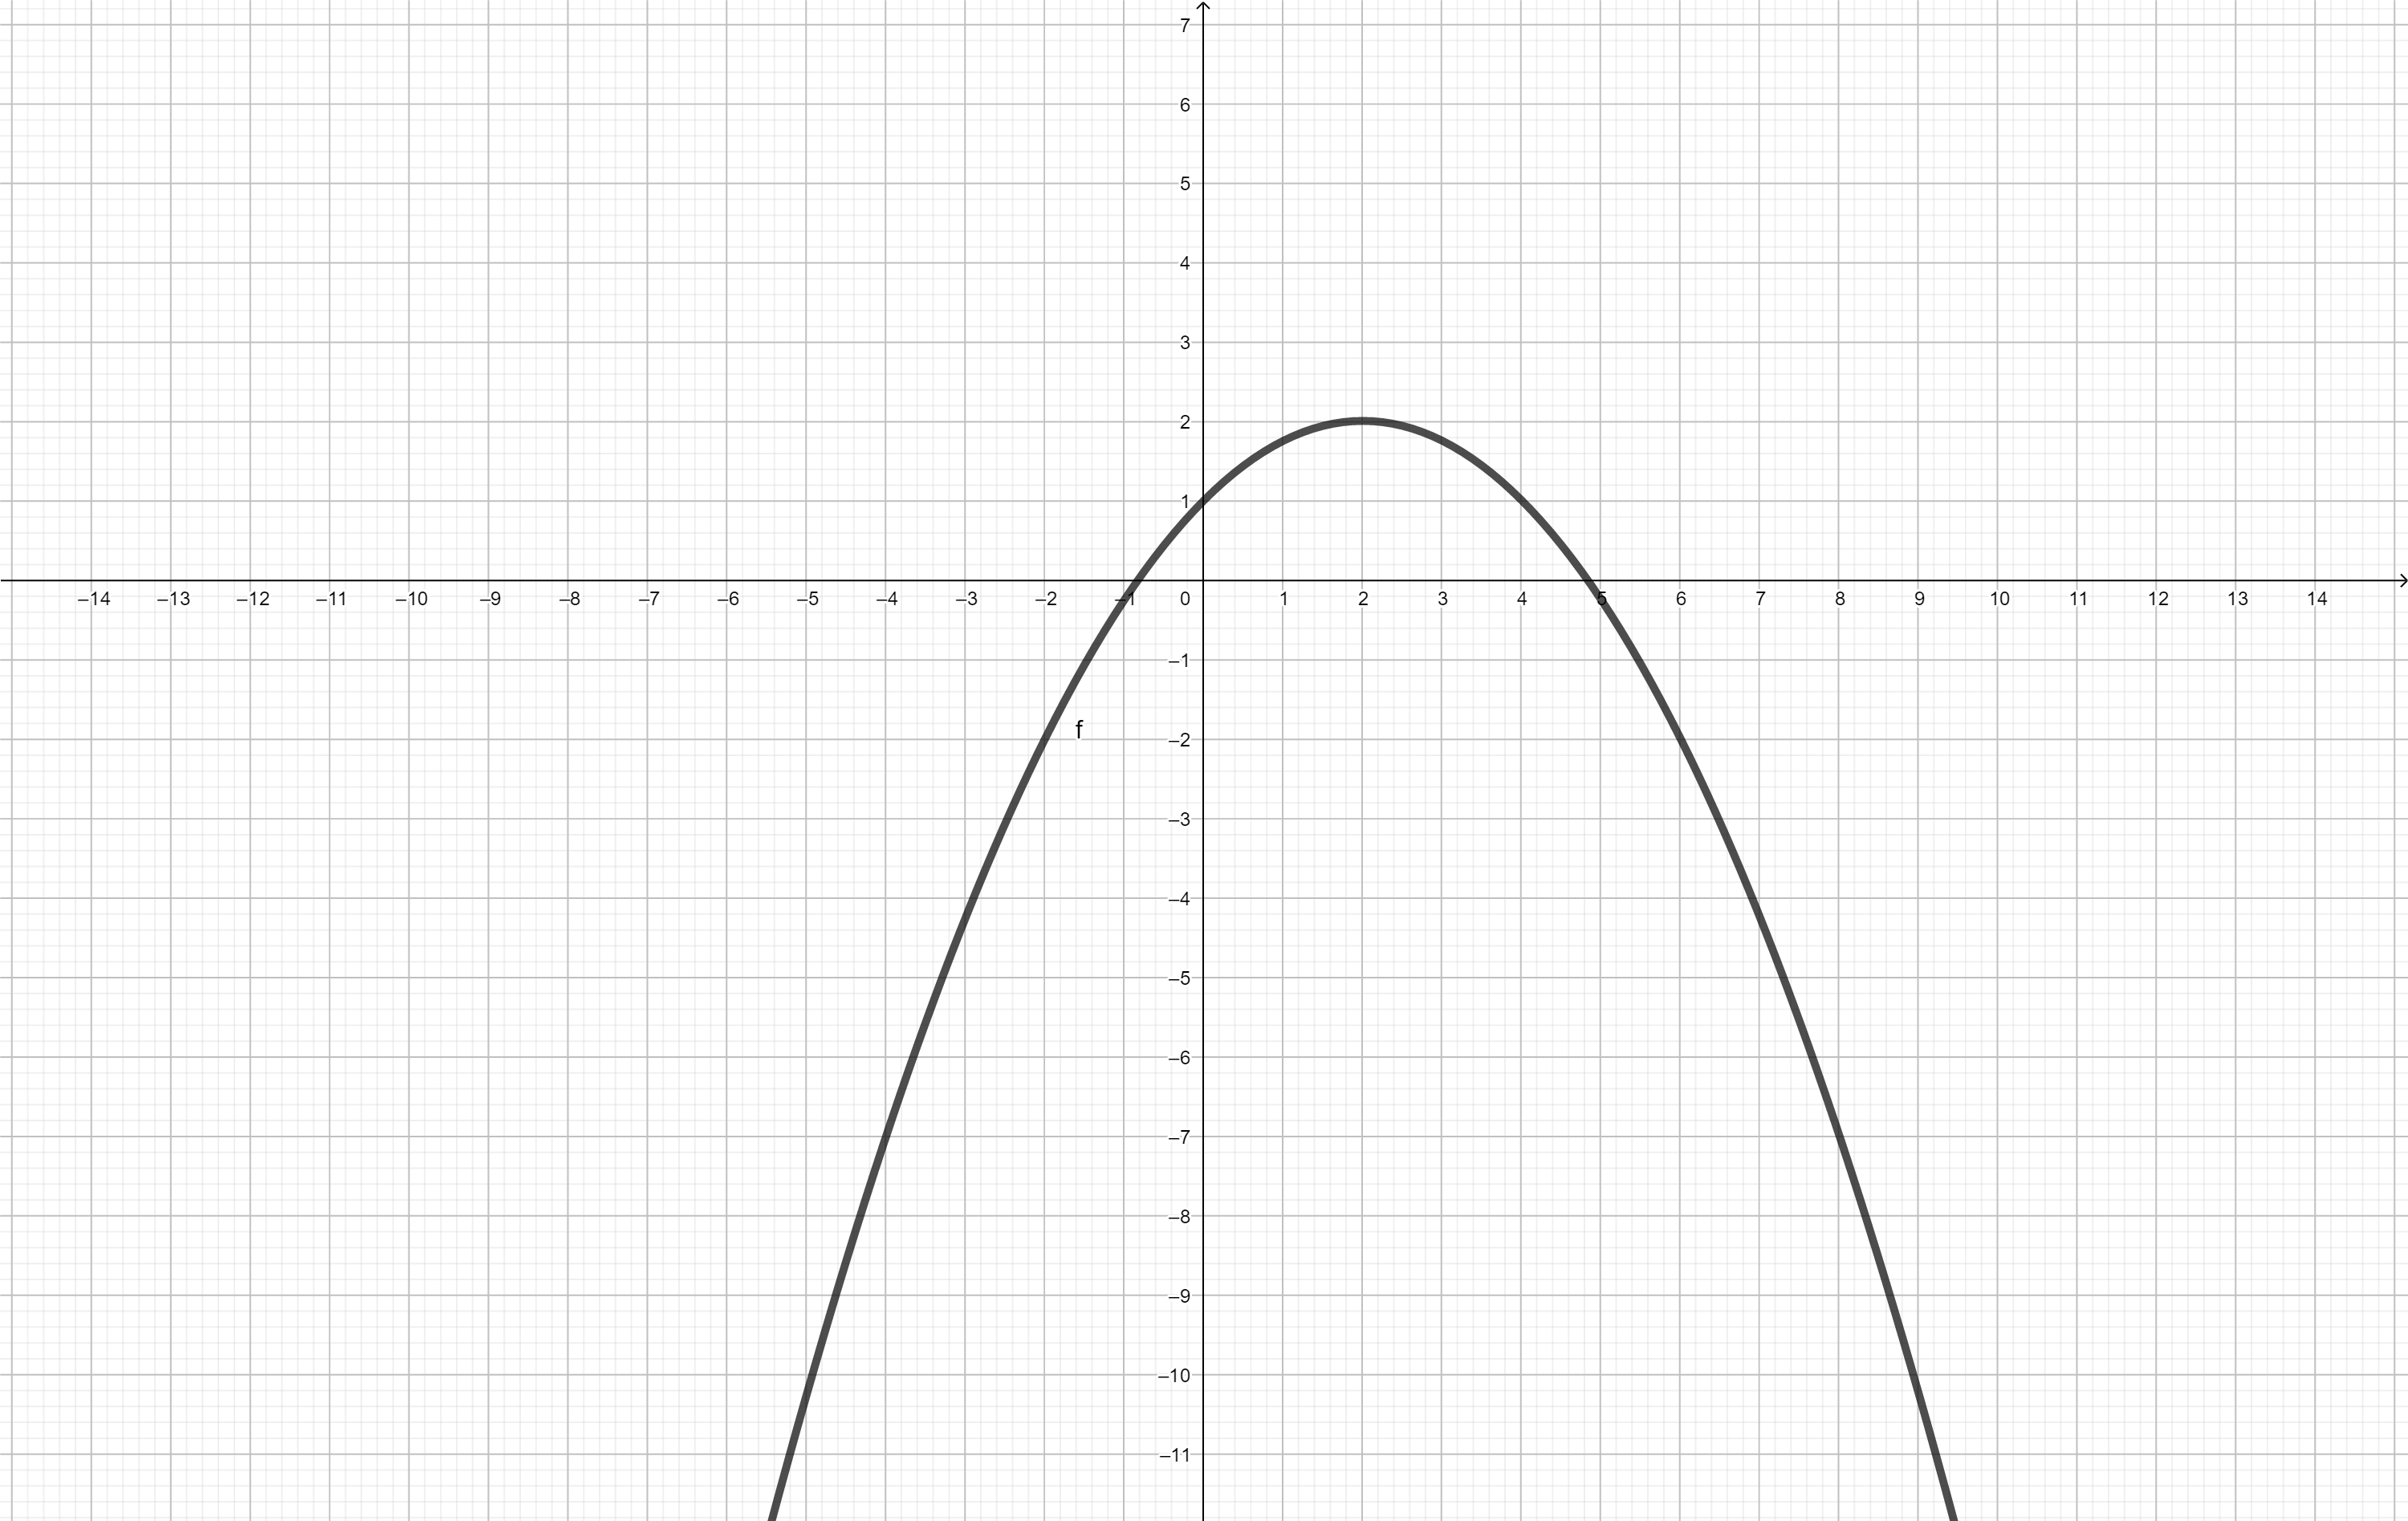
\includegraphics[width=4cm]{Bilder/G24}

\begin{addmargin}[-2cm]{0pt}
Hochpunkte: \\
Tiefpunkte: \\
Summe: \\
Wendepunkte:
\end{addmargin}

\paragraph{Grad 3:}\textcolor{white}{.}\\
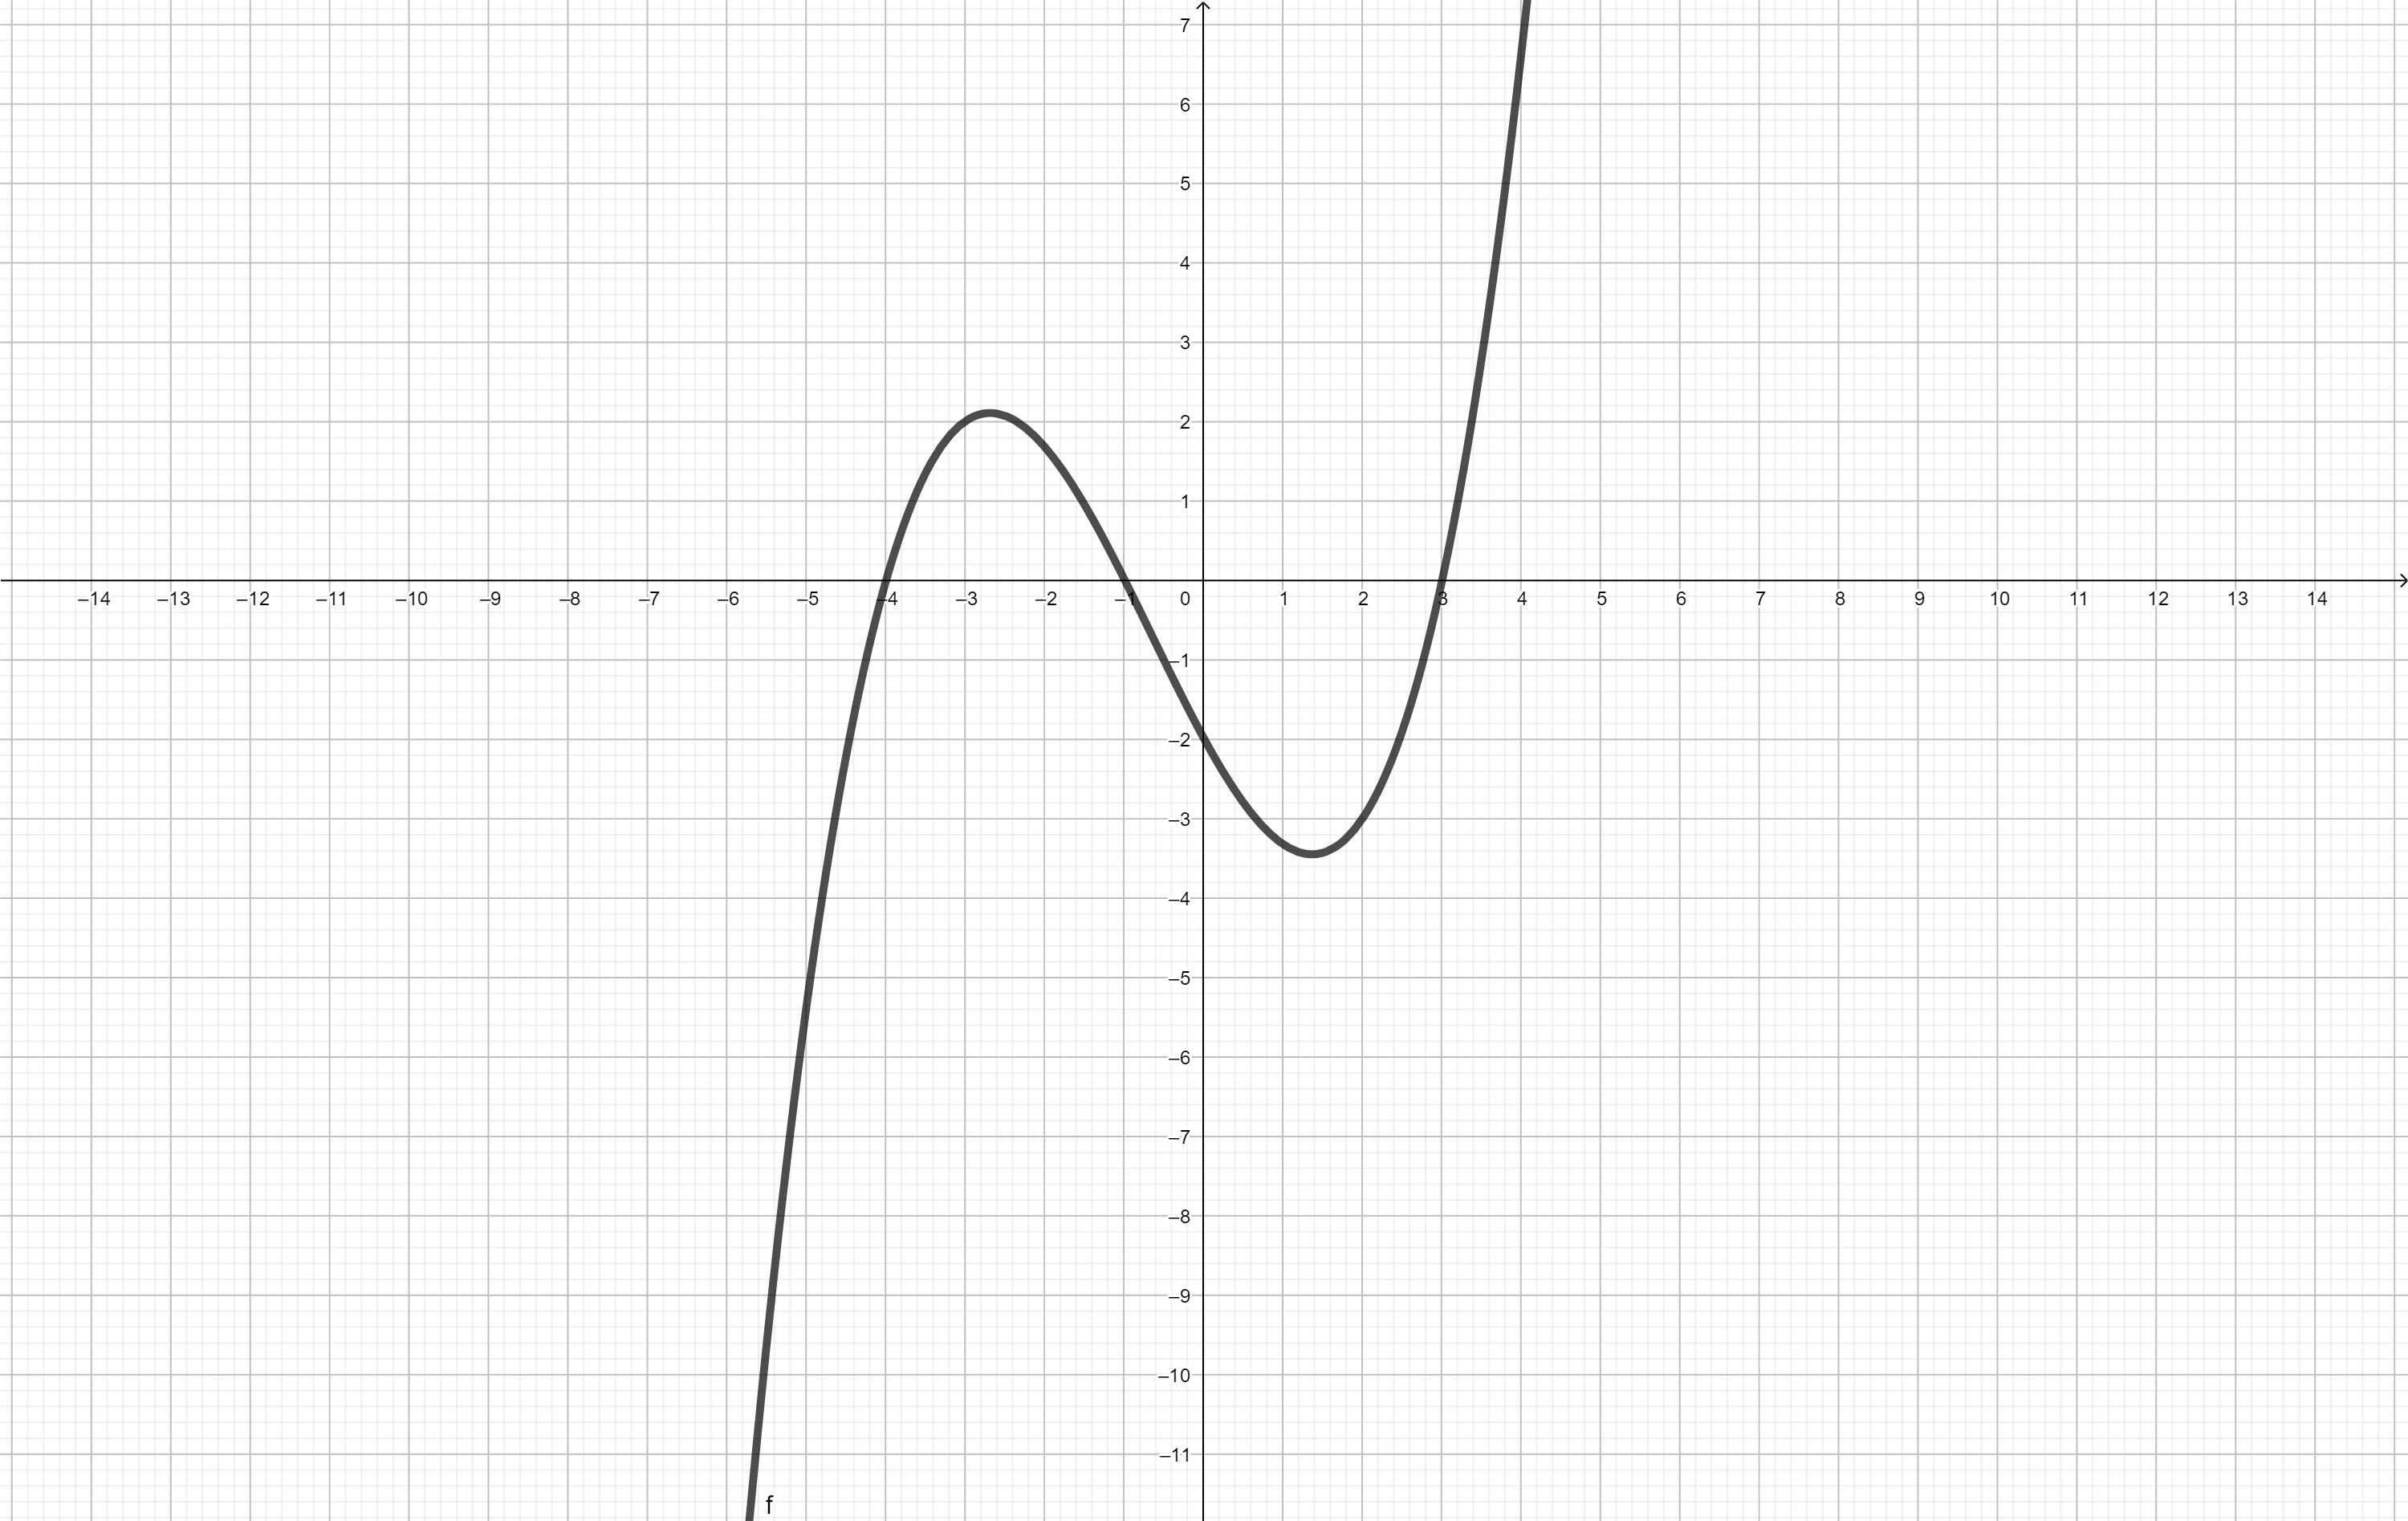
\includegraphics[width=4cm]{Bilder/G31}\hfill
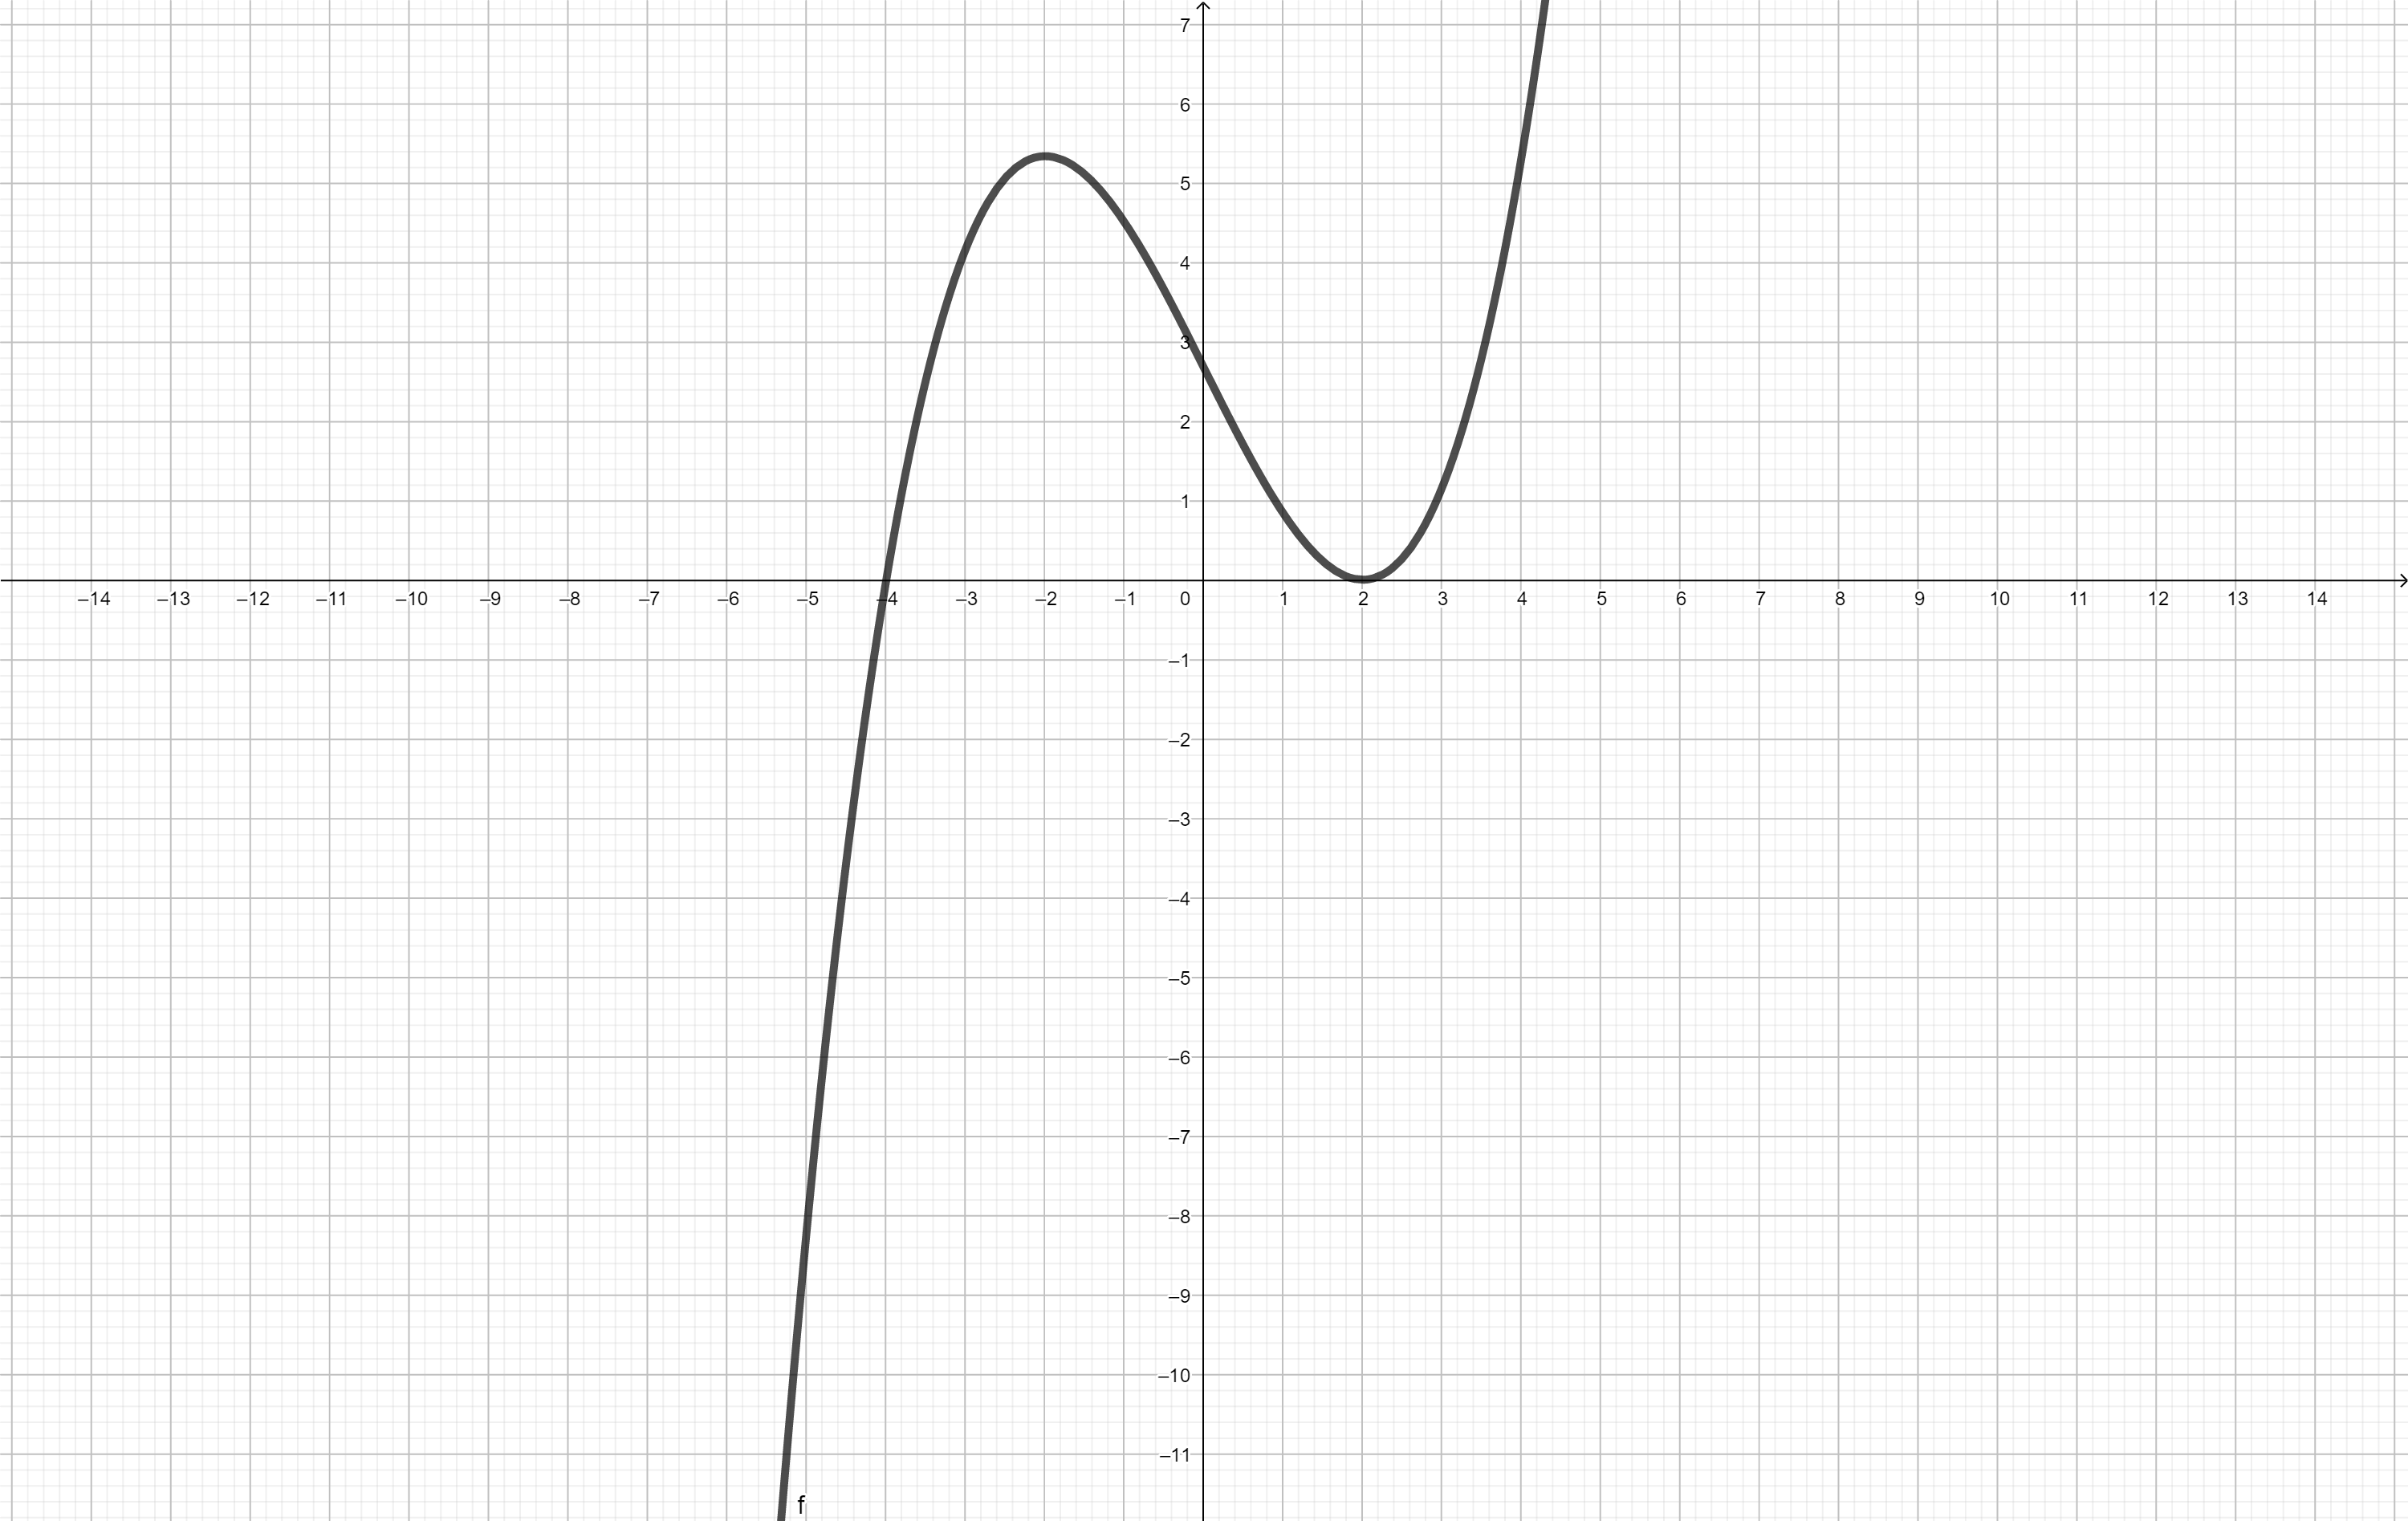
\includegraphics[width=4cm]{Bilder/G32}\hfill
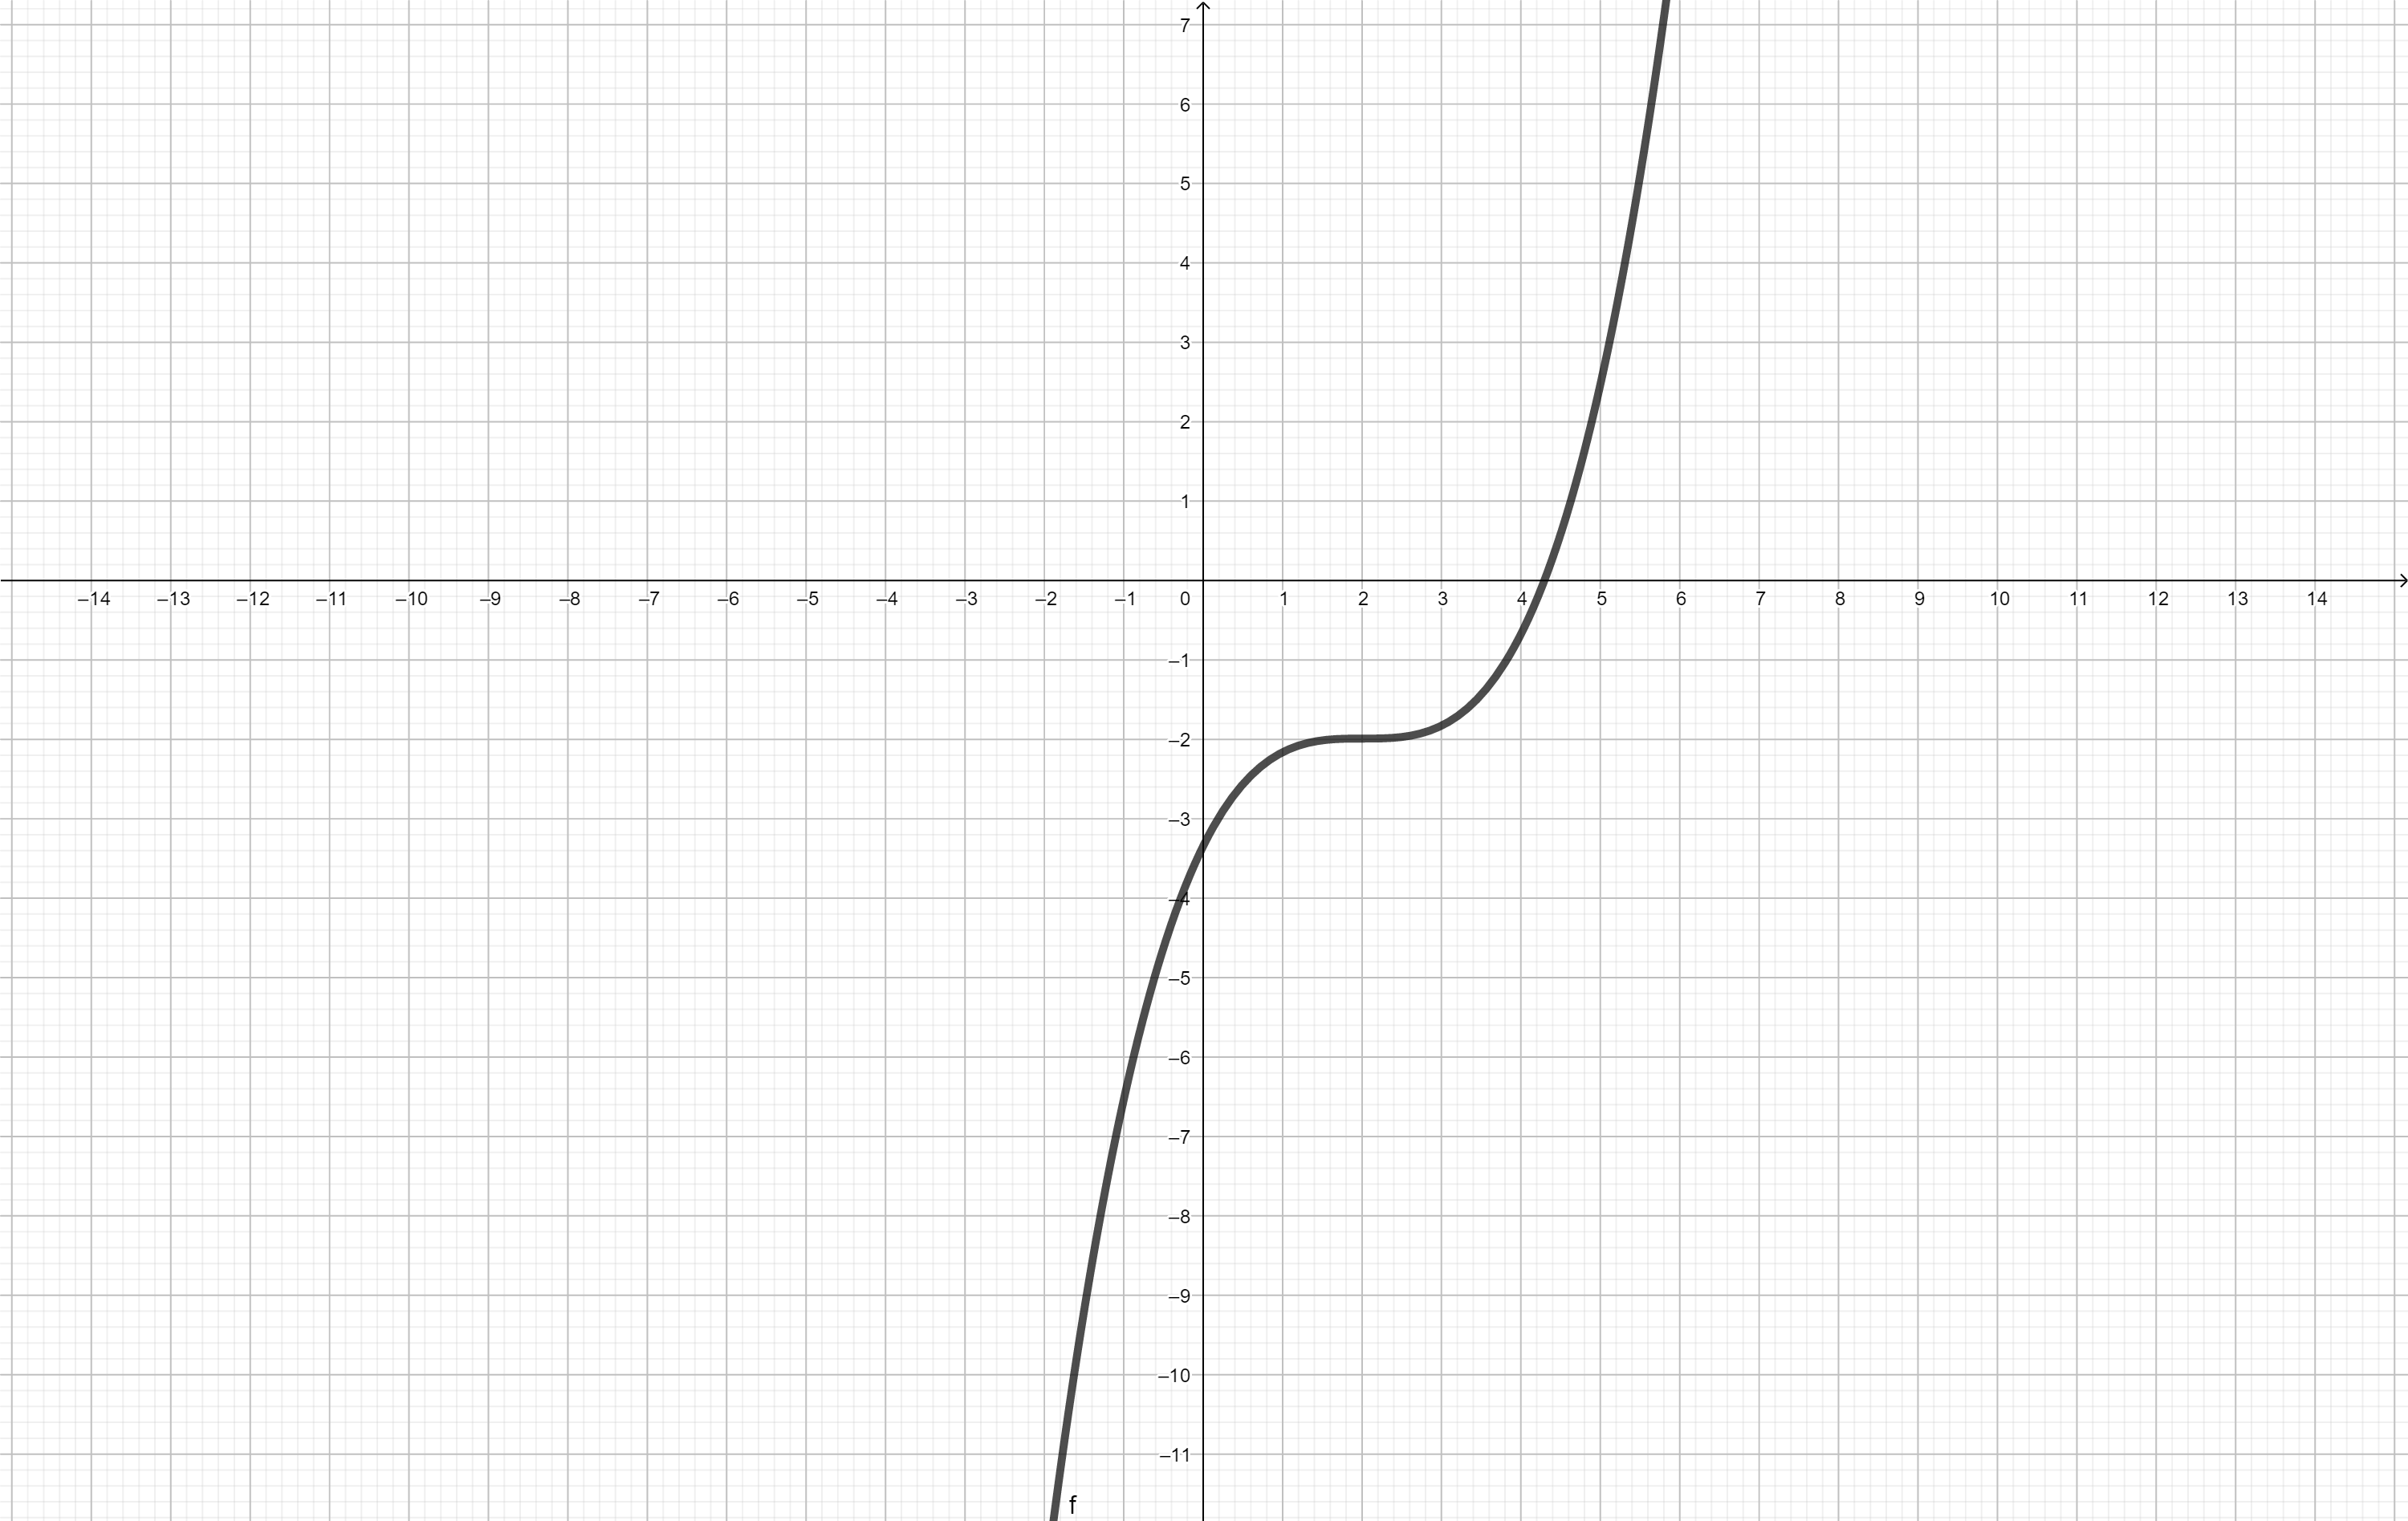
\includegraphics[width=4cm]{Bilder/G33}\hfill
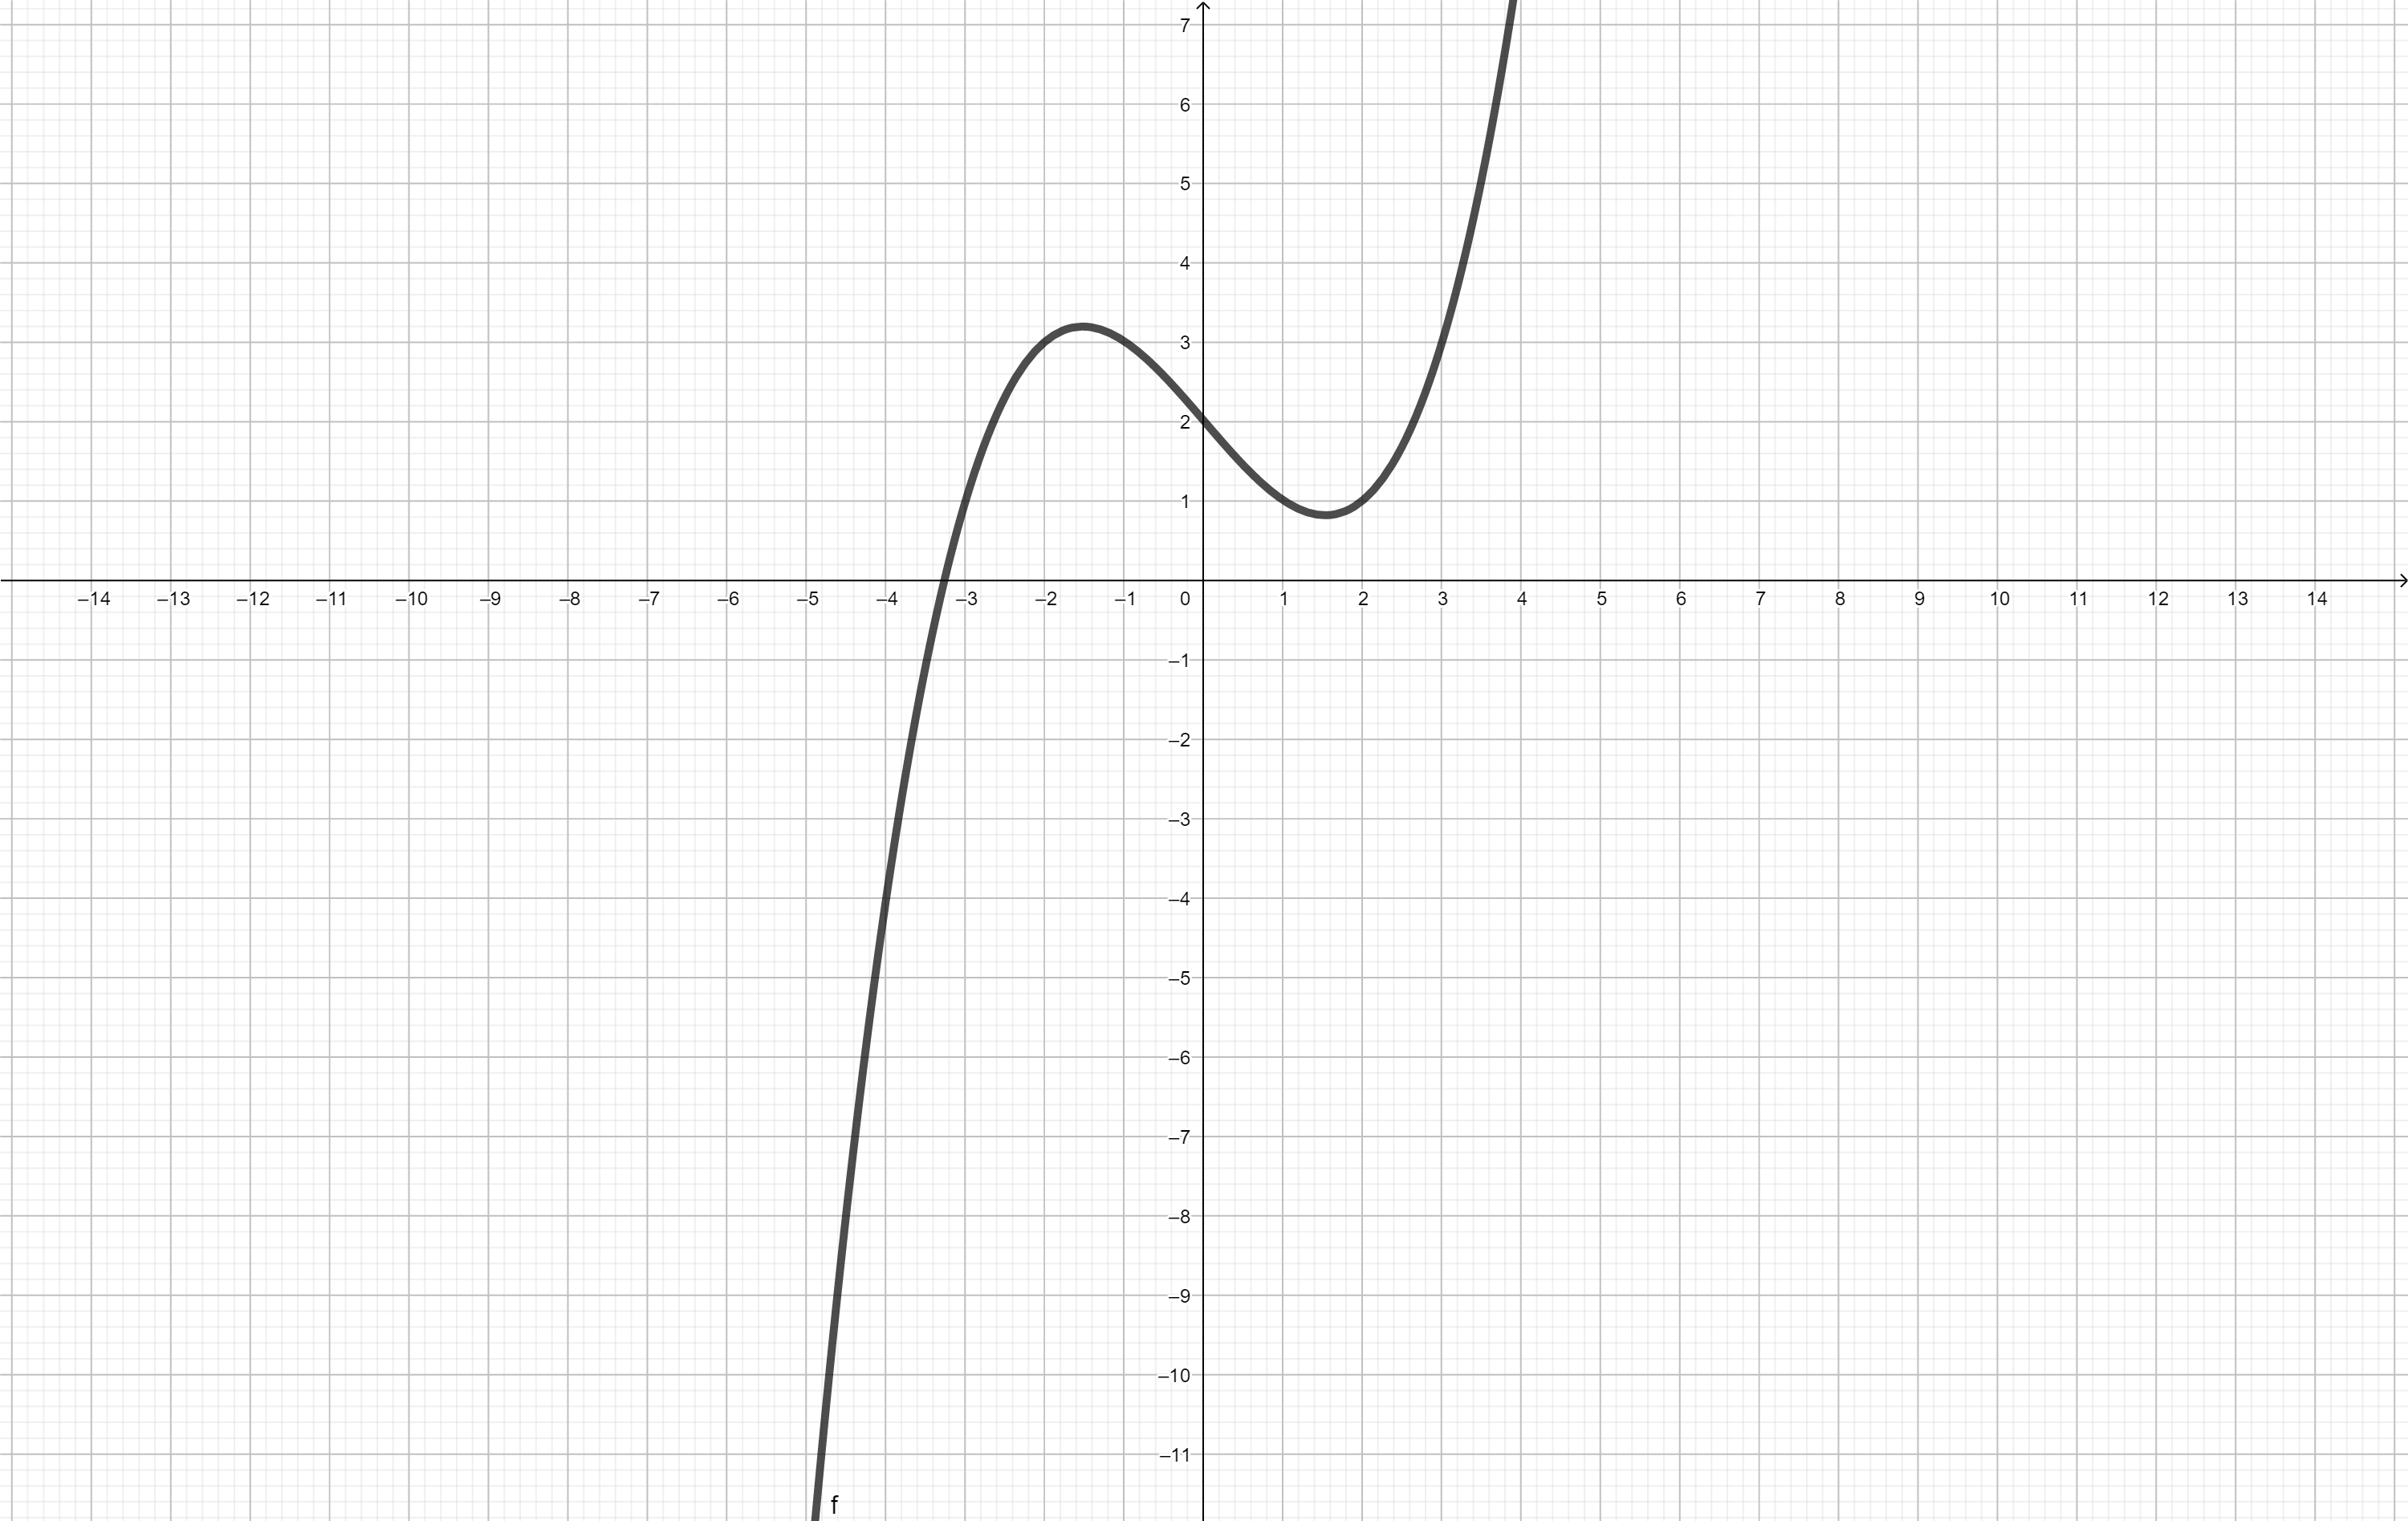
\includegraphics[width=4cm]{Bilder/G34}

\begin{addmargin}[-2cm]{0pt}
Hochpunkte: \\
Tiefpunkte: \\
Summe: \\
Wendepunkte:
\end{addmargin}

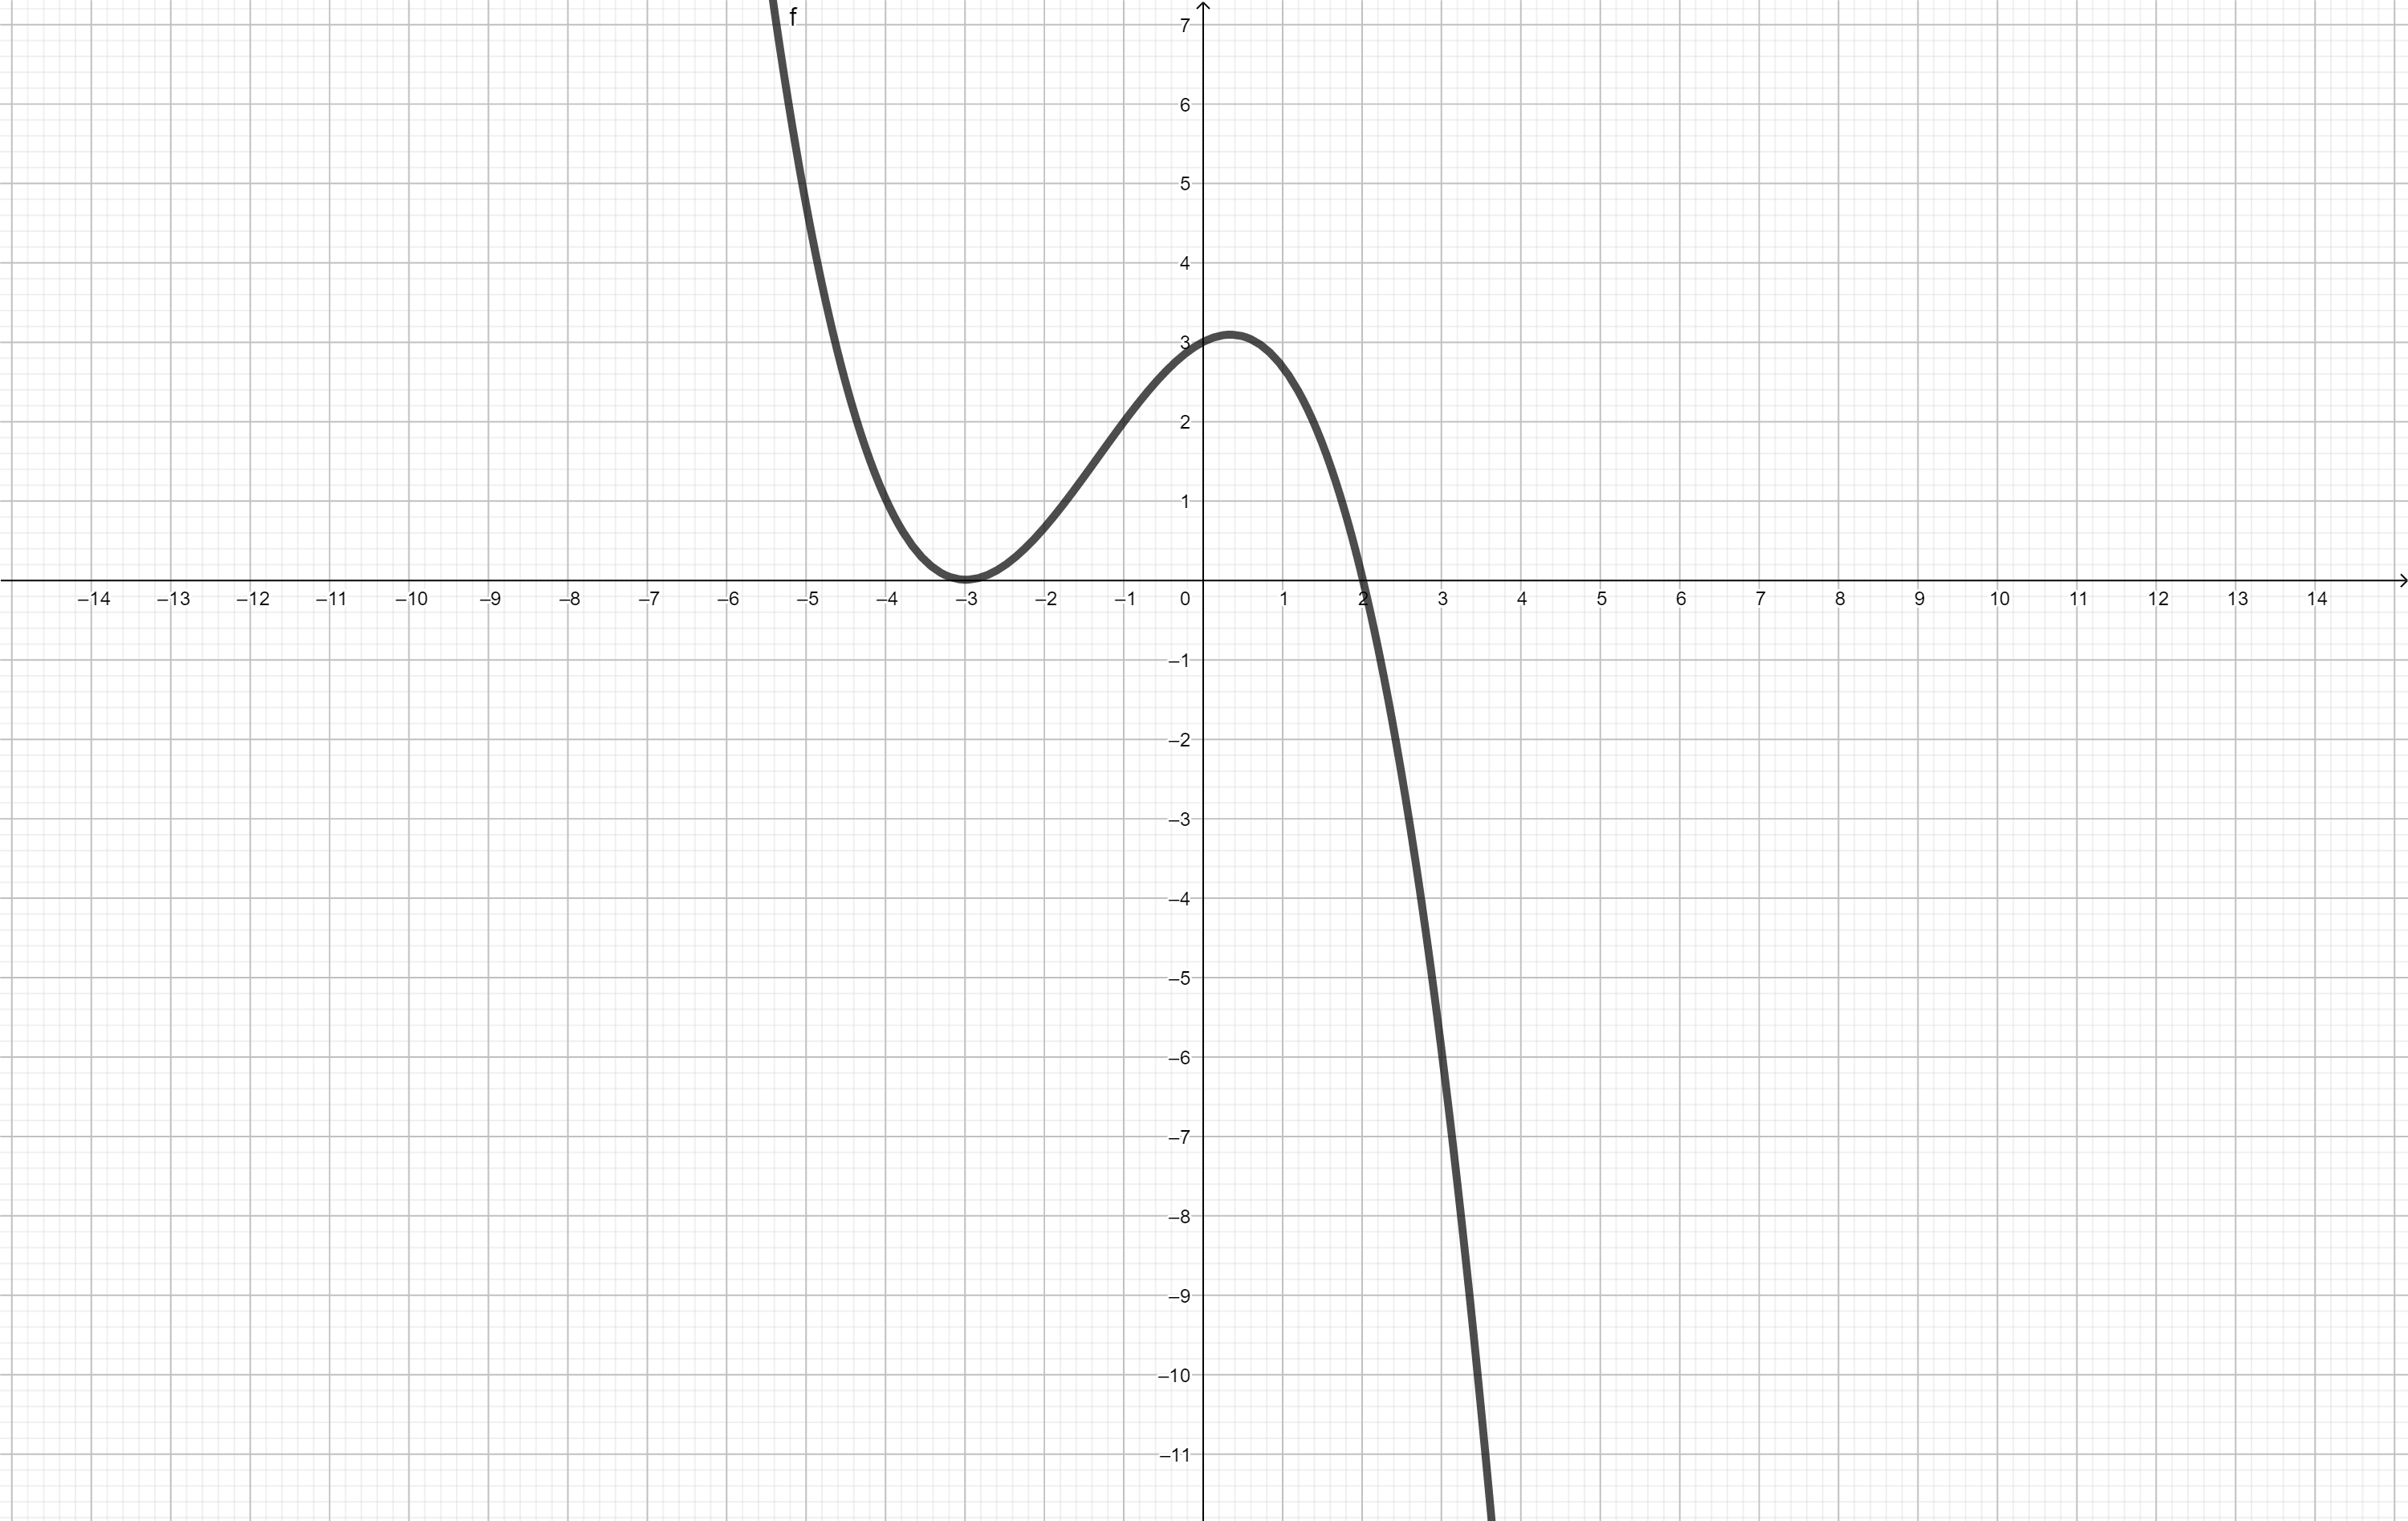
\includegraphics[width=4cm]{Bilder/G35}\hfill
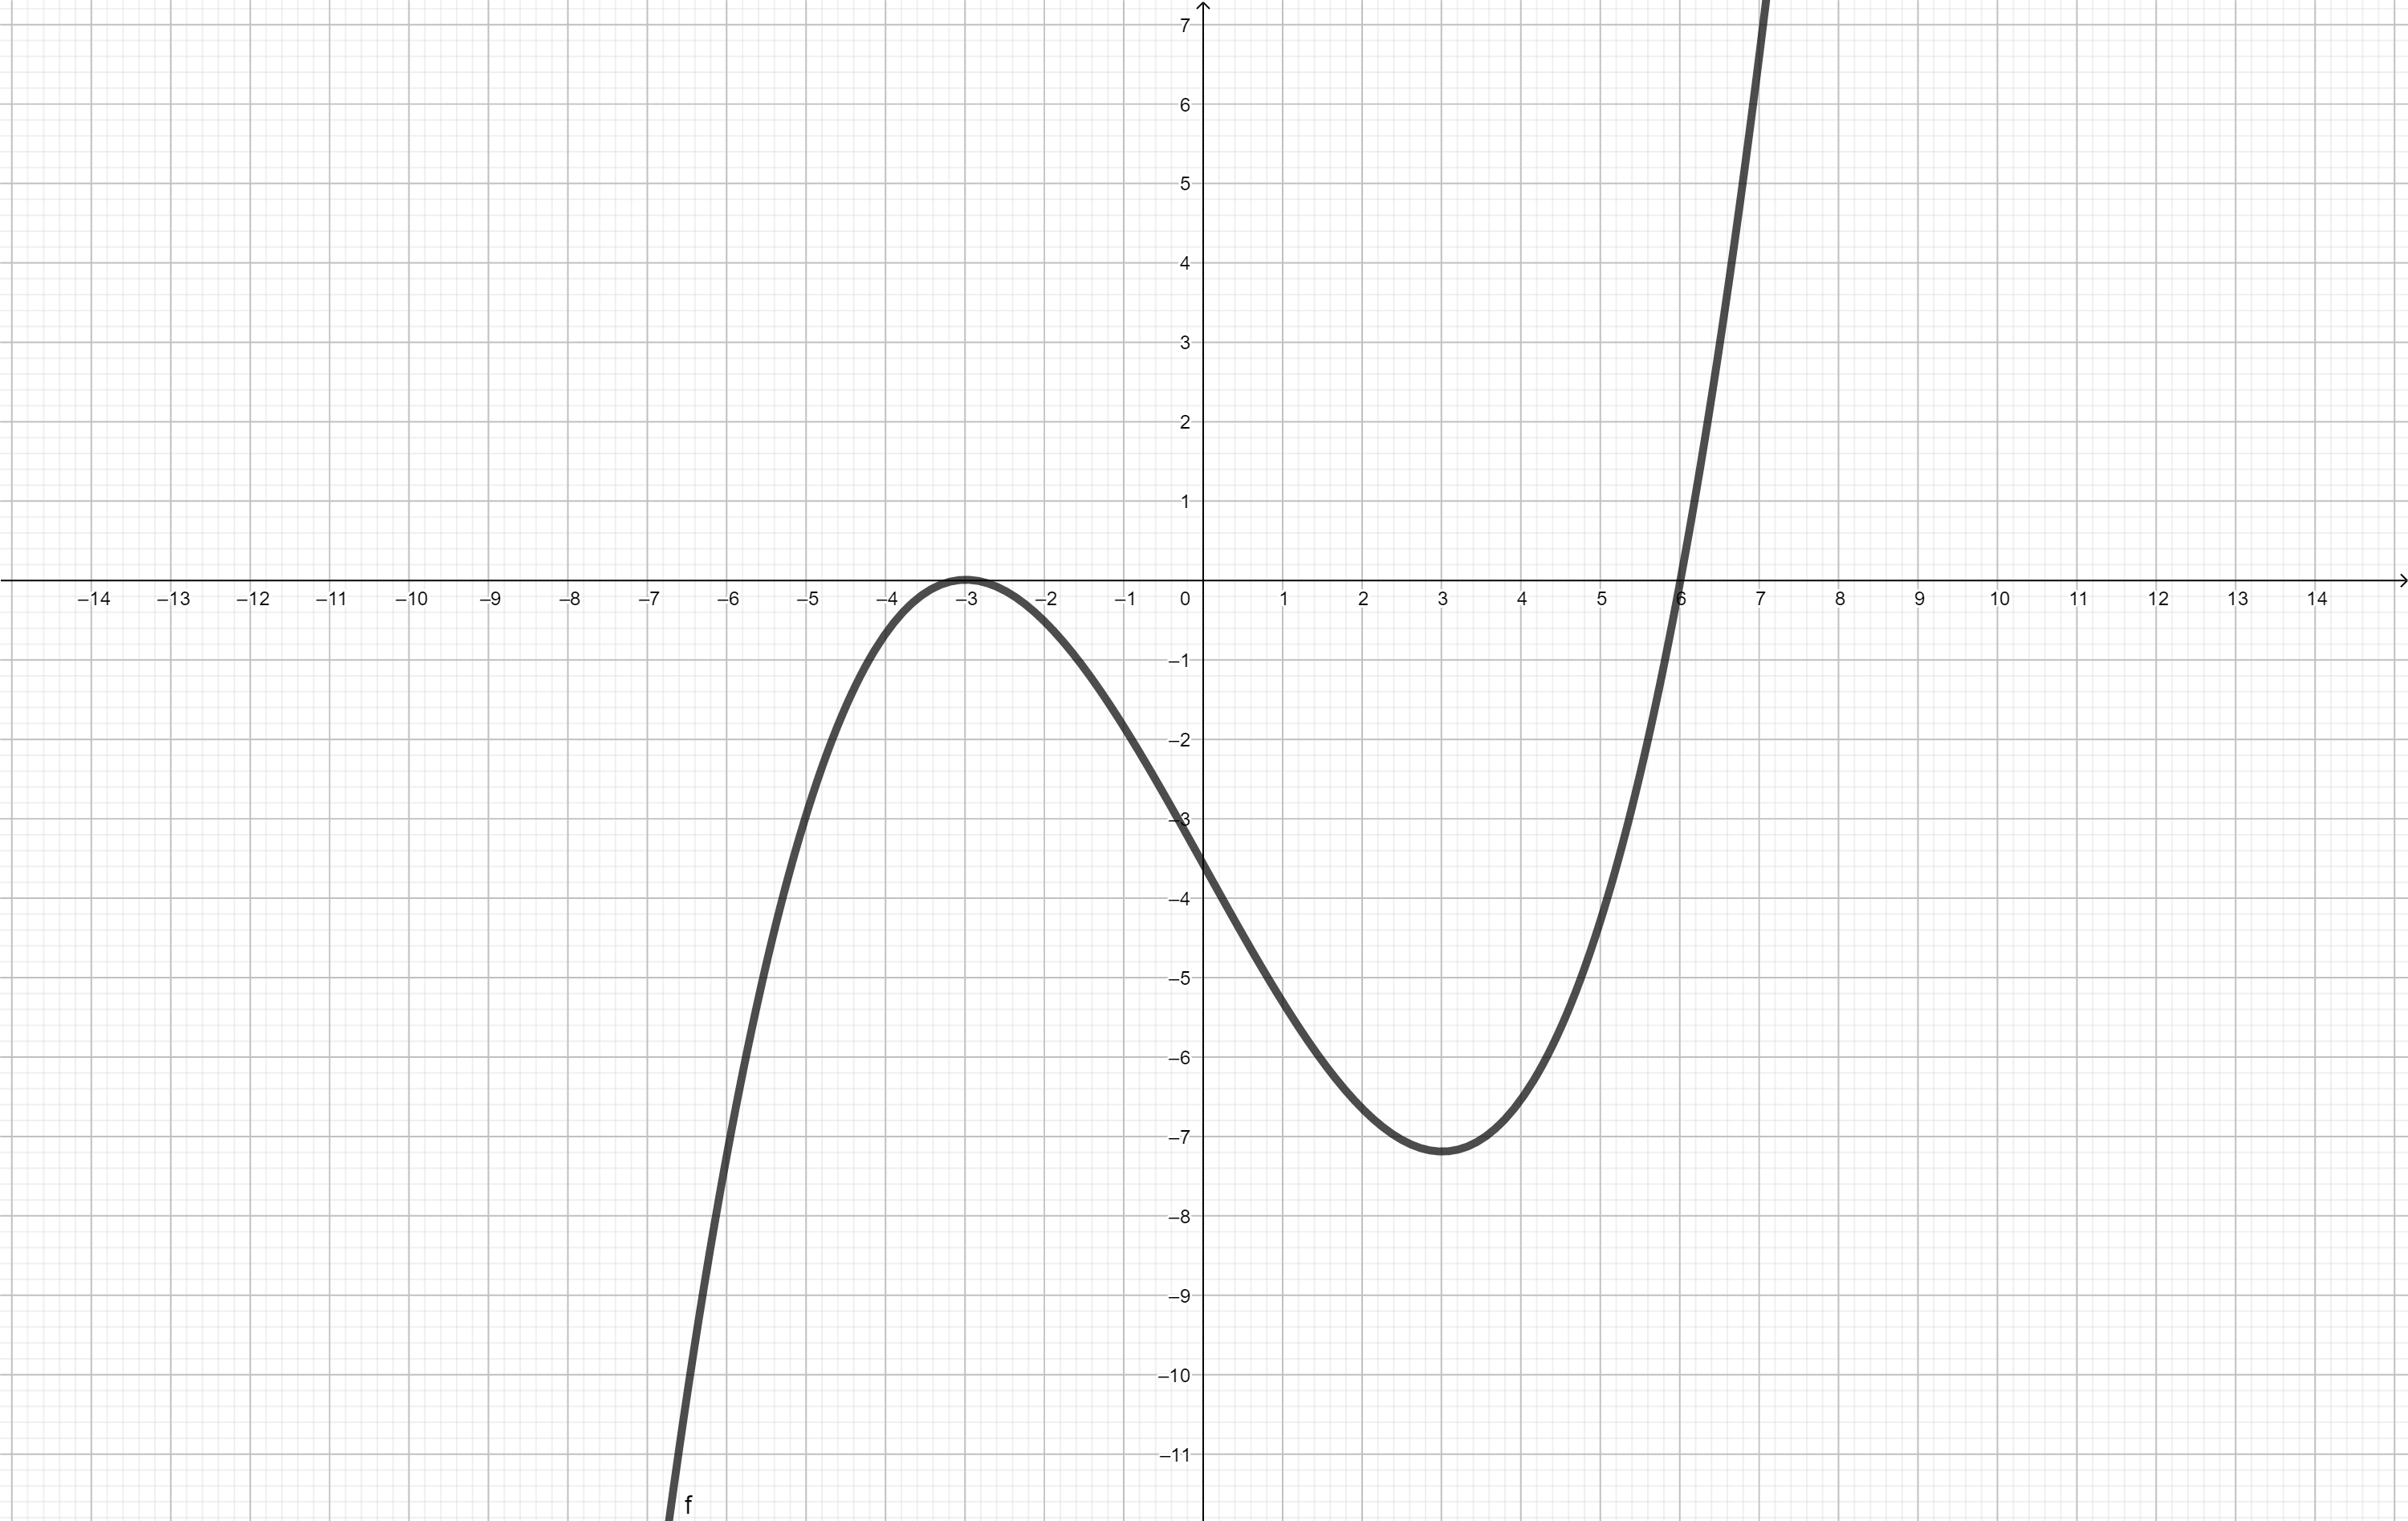
\includegraphics[width=4cm]{Bilder/G36}\hfill
\includegraphics[width=4cm]{Bilder/G37}\hfill
\includegraphics[width=4cm]{Bilder/G38}

\begin{addmargin}[-2cm]{0pt}
Hochpunkte: \\
Tiefpunkte: \\
Summe: \\
Wendepunkte:
\end{addmargin}

\newpage

\paragraph{Grad 4:}\textcolor{white}{.}\\
\includegraphics[width=4cm]{Bilder/G41}\hfill
\includegraphics[width=4cm]{Bilder/G42}\hfill
\includegraphics[width=4cm]{Bilder/G43}\hfill
\includegraphics[width=4cm]{Bilder/G44}

\begin{addmargin}[-2cm]{0pt}
Hochpunkte: \\
Tiefpunkte: \\
Summe: \\
Wendepunkte:
\end{addmargin}

\includegraphics[width=4cm]{Bilder/G45}\hfill
\includegraphics[width=4cm]{Bilder/G46}\hfill
\includegraphics[width=4cm]{Bilder/G47}\hfill
\includegraphics[width=4cm]{Bilder/G48}

\begin{addmargin}[-2cm]{0pt}
Hochpunkte: \\
Tiefpunkte: \\
Summe: \\
Wendepunkte:
\end{addmargin}

\paragraph{Grad 5:}\textcolor{white}{.}\\
\includegraphics[width=4cm]{Bilder/G51}\hfill
\includegraphics[width=4cm]{Bilder/G52}\hfill
\includegraphics[width=4cm]{Bilder/G53}\hfill
\includegraphics[width=4cm]{Bilder/G54}

\begin{addmargin}[-2cm]{0pt}
Hochpunkte: \\
Tiefpunkte: \\
Summe: \\
Wendepunkte:
\end{addmargin}

\includegraphics[width=4cm]{Bilder/G55}\hfill
\includegraphics[width=4cm]{Bilder/G56}\hfill
\includegraphics[width=4cm]{Bilder/G57}\hfill
\includegraphics[width=4cm]{Bilder/G58}

\begin{addmargin}[-2cm]{0pt}
Hochpunkte: \\
Tiefpunkte: \\
Summe: \\
Wendepunkte:
\end{addmargin}

\includegraphics[width=4cm]{Bilder/G59}\hfill
\includegraphics[width=4cm]{Bilder/G510}\hfill
\includegraphics[width=4cm]{Bilder/G511}\hfill
\includegraphics[width=4cm]{Bilder/G512}

\begin{addmargin}[-2cm]{0pt}
Hochpunkte: \\
Tiefpunkte: \\
Summe: \\
Wendepunkte:
\end{addmargin}


\end{document}